\documentclass[twoside]{book}

% Packages required by doxygen
\usepackage{calc}
\usepackage{doxygen}
\usepackage{graphicx}
\usepackage[utf8]{inputenc}
\usepackage{makeidx}
\usepackage{multicol}
\usepackage{multirow}
\usepackage{fixltx2e}
\PassOptionsToPackage{warn}{textcomp}
\usepackage{textcomp}
\usepackage[nointegrals]{wasysym}
\usepackage[table]{xcolor}

% Font selection
\usepackage[T1]{fontenc}
\usepackage{mathptmx}
\usepackage[scaled=.90]{helvet}
\usepackage{courier}
\usepackage{amssymb}
\usepackage{sectsty}
\renewcommand{\familydefault}{\sfdefault}
\allsectionsfont{%
  \fontseries{bc}\selectfont%
  \color{darkgray}%
}
\renewcommand{\DoxyLabelFont}{%
  \fontseries{bc}\selectfont%
  \color{darkgray}%
}
\newcommand{\+}{\discretionary{\mbox{\scriptsize$\hookleftarrow$}}{}{}}

% Page & text layout
\usepackage{geometry}
\geometry{%
  a4paper,%
  top=2.5cm,%
  bottom=2.5cm,%
  left=2.5cm,%
  right=2.5cm%
}
\tolerance=750
\hfuzz=15pt
\hbadness=750
\setlength{\emergencystretch}{15pt}
\setlength{\parindent}{0cm}
\setlength{\parskip}{0.2cm}
\makeatletter
\renewcommand{\paragraph}{%
  \@startsection{paragraph}{4}{0ex}{-1.0ex}{1.0ex}{%
    \normalfont\normalsize\bfseries\SS@parafont%
  }%
}
\renewcommand{\subparagraph}{%
  \@startsection{subparagraph}{5}{0ex}{-1.0ex}{1.0ex}{%
    \normalfont\normalsize\bfseries\SS@subparafont%
  }%
}
\makeatother

% Headers & footers
\usepackage{fancyhdr}
\pagestyle{fancyplain}
\fancyhead[LE]{\fancyplain{}{\bfseries\thepage}}
\fancyhead[CE]{\fancyplain{}{}}
\fancyhead[RE]{\fancyplain{}{\bfseries\leftmark}}
\fancyhead[LO]{\fancyplain{}{\bfseries\rightmark}}
\fancyhead[CO]{\fancyplain{}{}}
\fancyhead[RO]{\fancyplain{}{\bfseries\thepage}}
\fancyfoot[LE]{\fancyplain{}{}}
\fancyfoot[CE]{\fancyplain{}{}}
\fancyfoot[RE]{\fancyplain{}{\bfseries\scriptsize Generated on Tue Jul 15 2014 14\+:14\+:19 for S\+C 3.\+6 by Doxygen }}
\fancyfoot[LO]{\fancyplain{}{\bfseries\scriptsize Generated on Tue Jul 15 2014 14\+:14\+:19 for S\+C 3.\+6 by Doxygen }}
\fancyfoot[CO]{\fancyplain{}{}}
\fancyfoot[RO]{\fancyplain{}{}}
\renewcommand{\footrulewidth}{0.4pt}
\renewcommand{\chaptermark}[1]{%
  \markboth{#1}{}%
}
\renewcommand{\sectionmark}[1]{%
  \markright{\thesection\ #1}%
}

% Indices & bibliography
\usepackage{natbib}
\usepackage[titles]{tocloft}
\setcounter{tocdepth}{3}
\setcounter{secnumdepth}{5}
\makeindex

% Hyperlinks (required, but should be loaded last)
\usepackage{ifpdf}
\ifpdf
  \usepackage[pdftex,pagebackref=true]{hyperref}
\else
  \usepackage[ps2pdf,pagebackref=true]{hyperref}
\fi
\hypersetup{%
  colorlinks=true,%
  linkcolor=blue,%
  citecolor=blue,%
  unicode%
}

% Custom commands
\newcommand{\clearemptydoublepage}{%
  \newpage{\pagestyle{empty}\cleardoublepage}%
}


%===== C O N T E N T S =====

\begin{document}

% Titlepage & ToC
\hypersetup{pageanchor=false,
             bookmarks=true,
             bookmarksnumbered=true,
             pdfencoding=unicode
            }
\pagenumbering{roman}
\begin{titlepage}
\vspace*{7cm}
\begin{center}%
{\Large S\+C 3.6 }\\
\vspace*{1cm}
{\large Generated by Doxygen 1.8.7}\\
\vspace*{0.5cm}
{\small Tue Jul 15 2014 14:14:19}\\
\end{center}
\end{titlepage}
\clearemptydoublepage
\tableofcontents
\clearemptydoublepage
\pagenumbering{arabic}
\hypersetup{pageanchor=true}

%--- Begin generated contents ---
\chapter{Deprecated List}
\label{deprecated}
\hypertarget{deprecated}{}

\begin{DoxyRefList}
\item[\label{deprecated__deprecated000001}%
\hypertarget{deprecated__deprecated000001}{}%
Member \hyperlink{class_total_energy_calculator_a5b1555512d0d6891a77bf7d036df5d35}{Total\+Energy\+Calculator\+:\+:exter\+Atre} (double $\ast$ndist, int numpatch, double halfl)]
\end{DoxyRefList}
\chapter{Namespace Index}
\section{Namespace List}
Here is a list of all namespaces with brief descriptions\+:\begin{DoxyCompactList}
\item\contentsline{section}{\hyperlink{namespaceprint_stat}{print\+Stat} }{\pageref{namespaceprint_stat}}{}
\end{DoxyCompactList}

\chapter{Class Index}
\section{Class List}
Here are the classes, structs, unions and interfaces with brief descriptions\+:\begin{DoxyCompactList}
\item\contentsline{section}{\hyperlink{struct_cluster}{Cluster} \\*All the particles of one cluster }{\pageref{struct_cluster}}{}
\item\contentsline{section}{\hyperlink{class_conf}{Conf} \\*Configuration of the system }{\pageref{class_conf}}{}
\item\contentsline{section}{\hyperlink{class_disp}{Disp} \\*Define step size and acceptance ratio statistics }{\pageref{class_disp}}{}
\item\contentsline{section}{\hyperlink{class_exters}{Exters} }{\pageref{class_exters}}{}
\item\contentsline{section}{\hyperlink{struct_file_names}{File\+Names} }{\pageref{struct_file_names}}{}
\item\contentsline{section}{\hyperlink{class_ia__param}{Ia\+\_\+param} \\*Contatins properties and parameters of particle types }{\pageref{class_ia__param}}{}
\item\contentsline{section}{\hyperlink{class_inicializer}{Inicializer} }{\pageref{class_inicializer}}{}
\item\contentsline{section}{\hyperlink{class_m_c_sim_system}{M\+C\+Sim\+System} }{\pageref{class_m_c_sim_system}}{}
\item\contentsline{section}{\hyperlink{class_mesh}{Mesh} \\*\hyperlink{class_mesh}{Mesh} for hole order parameter }{\pageref{class_mesh}}{}
\item\contentsline{section}{\hyperlink{class_molecule}{Molecule} \\*This structure is for io only }{\pageref{class_molecule}}{}
\item\contentsline{section}{\hyperlink{class_molecule_params}{Molecule\+Params} \\*Parameters for inner interaction in chains }{\pageref{class_molecule_params}}{}
\item\contentsline{section}{\hyperlink{class_move_creator}{Move\+Creator} }{\pageref{class_move_creator}}{}
\item\contentsline{section}{\hyperlink{struct_option}{Option} }{\pageref{struct_option}}{}
\item\contentsline{section}{\hyperlink{class_pair_energy_calculator}{Pair\+Energy\+Calculator} }{\pageref{class_pair_energy_calculator}}{}
\item\contentsline{section}{\hyperlink{class_particle}{Particle} \\*Define a particle }{\pageref{class_particle}}{}
\item\contentsline{section}{\hyperlink{class_quat}{Quat} }{\pageref{class_quat}}{}
\item\contentsline{section}{\hyperlink{class_ran2}{Ran2} }{\pageref{class_ran2}}{}
\item\contentsline{section}{\hyperlink{class_sim}{Sim} \\*Should contain mostly all the simulation options and variables }{\pageref{class_sim}}{}
\item\contentsline{section}{\hyperlink{class_topo}{Topo} }{\pageref{class_topo}}{}
\item\contentsline{section}{\hyperlink{class_total_energy_calculator}{Total\+Energy\+Calculator} }{\pageref{class_total_energy_calculator}}{}
\item\contentsline{section}{\hyperlink{class_updater}{Updater} }{\pageref{class_updater}}{}
\item\contentsline{section}{\hyperlink{class_vector}{Vector} }{\pageref{class_vector}}{}
\item\contentsline{section}{\hyperlink{class_wang_landau}{Wang\+Landau} }{\pageref{class_wang_landau}}{}
\end{DoxyCompactList}

\chapter{File Index}
\section{File List}
Here is a list of all files with brief descriptions\+:\begin{DoxyCompactList}
\item\contentsline{section}{sc\+O\+O\+P/\hyperlink{main_8cpp}{main.\+cpp} }{\pageref{main_8cpp}}{}
\item\contentsline{section}{sc\+O\+O\+P/mc/\hyperlink{inicializer_8cpp}{inicializer.\+cpp} }{\pageref{inicializer_8cpp}}{}
\item\contentsline{section}{sc\+O\+O\+P/mc/\hyperlink{inicializer_8h}{inicializer.\+h} }{\pageref{inicializer_8h}}{}
\item\contentsline{section}{sc\+O\+O\+P/mc/\hyperlink{math__calc_8h}{math\+\_\+calc.\+h} }{\pageref{math__calc_8h}}{}
\item\contentsline{section}{sc\+O\+O\+P/mc/\hyperlink{mcsimsystem_8cpp}{mcsimsystem.\+cpp} }{\pageref{mcsimsystem_8cpp}}{}
\item\contentsline{section}{sc\+O\+O\+P/mc/\hyperlink{mcsimsystem_8h}{mcsimsystem.\+h} }{\pageref{mcsimsystem_8h}}{}
\item\contentsline{section}{sc\+O\+O\+P/mc/\hyperlink{mesh_8cpp}{mesh.\+cpp} }{\pageref{mesh_8cpp}}{}
\item\contentsline{section}{sc\+O\+O\+P/mc/\hyperlink{mesh_8h}{mesh.\+h} }{\pageref{mesh_8h}}{}
\item\contentsline{section}{sc\+O\+O\+P/mc/\hyperlink{movecreator_8cpp}{movecreator.\+cpp} }{\pageref{movecreator_8cpp}}{}
\item\contentsline{section}{sc\+O\+O\+P/mc/\hyperlink{movecreator_8h}{movecreator.\+h} }{\pageref{movecreator_8h}}{}
\item\contentsline{section}{sc\+O\+O\+P/mc/\hyperlink{_move_creator_mesh_8cpp}{Move\+Creator\+Mesh.\+cpp} }{\pageref{_move_creator_mesh_8cpp}}{}
\item\contentsline{section}{sc\+O\+O\+P/mc/\hyperlink{mygetline_8h}{mygetline.\+h} }{\pageref{mygetline_8h}}{}
\item\contentsline{section}{sc\+O\+O\+P/mc/\hyperlink{mygetline2_8cpp}{mygetline2.\+cpp} }{\pageref{mygetline2_8cpp}}{}
\item\contentsline{section}{sc\+O\+O\+P/mc/\hyperlink{pairenergycalculator_8cpp}{pairenergycalculator.\+cpp} }{\pageref{pairenergycalculator_8cpp}}{}
\item\contentsline{section}{sc\+O\+O\+P/mc/\hyperlink{pairenergycalculator_8h}{pairenergycalculator.\+h} }{\pageref{pairenergycalculator_8h}}{}
\item\contentsline{section}{sc\+O\+O\+P/mc/\hyperlink{print_stat_8cpp}{print\+Stat.\+cpp} }{\pageref{print_stat_8cpp}}{}
\item\contentsline{section}{sc\+O\+O\+P/mc/\hyperlink{print_stat_8h}{print\+Stat.\+h} }{\pageref{print_stat_8h}}{}
\item\contentsline{section}{sc\+O\+O\+P/mc/\hyperlink{ran2_8cpp}{ran2.\+cpp} }{\pageref{ran2_8cpp}}{}
\item\contentsline{section}{sc\+O\+O\+P/mc/\hyperlink{ran2_8h}{ran2.\+h} }{\pageref{ran2_8h}}{}
\item\contentsline{section}{sc\+O\+O\+P/mc/\hyperlink{simlib_8cpp}{simlib.\+cpp} }{\pageref{simlib_8cpp}}{}
\item\contentsline{section}{sc\+O\+O\+P/mc/\hyperlink{simlib_8h}{simlib.\+h} }{\pageref{simlib_8h}}{}
\item\contentsline{section}{sc\+O\+O\+P/mc/\hyperlink{totalenergycalculator_8cpp}{totalenergycalculator.\+cpp} }{\pageref{totalenergycalculator_8cpp}}{}
\item\contentsline{section}{sc\+O\+O\+P/mc/\hyperlink{totalenergycalculator_8h}{totalenergycalculator.\+h} }{\pageref{totalenergycalculator_8h}}{}
\item\contentsline{section}{sc\+O\+O\+P/mc/\hyperlink{updater_8cpp}{updater.\+cpp} }{\pageref{updater_8cpp}}{}
\item\contentsline{section}{sc\+O\+O\+P/mc/\hyperlink{updater_8h}{updater.\+h} }{\pageref{updater_8h}}{}
\item\contentsline{section}{sc\+O\+O\+P/mc/\hyperlink{wanglandau_8cpp}{wanglandau.\+cpp} }{\pageref{wanglandau_8cpp}}{}
\item\contentsline{section}{sc\+O\+O\+P/mc/\hyperlink{wanglandau_8h}{wanglandau.\+h} }{\pageref{wanglandau_8h}}{}
\item\contentsline{section}{sc\+O\+O\+P/structures/\hyperlink{_conf_8cpp}{Conf.\+cpp} }{\pageref{_conf_8cpp}}{}
\item\contentsline{section}{sc\+O\+O\+P/structures/\hyperlink{_conf_8h}{Conf.\+h} }{\pageref{_conf_8h}}{}
\item\contentsline{section}{sc\+O\+O\+P/structures/\hyperlink{macros_8h}{macros.\+h} }{\pageref{macros_8h}}{}
\item\contentsline{section}{sc\+O\+O\+P/structures/\hyperlink{particle_8cpp}{particle.\+cpp} }{\pageref{particle_8cpp}}{}
\item\contentsline{section}{sc\+O\+O\+P/structures/\hyperlink{particle_8h}{particle.\+h} }{\pageref{particle_8h}}{}
\item\contentsline{section}{sc\+O\+O\+P/structures/\hyperlink{particlestore_8cpp}{particlestore.\+cpp} }{\pageref{particlestore_8cpp}}{}
\item\contentsline{section}{sc\+O\+O\+P/structures/\hyperlink{particlestore_8h}{particlestore.\+h} }{\pageref{particlestore_8h}}{}
\item\contentsline{section}{sc\+O\+O\+P/structures/\hyperlink{quaternion_8h}{quaternion.\+h} }{\pageref{quaternion_8h}}{}
\item\contentsline{section}{sc\+O\+O\+P/structures/\hyperlink{sim_8h}{sim.\+h} }{\pageref{sim_8h}}{}
\item\contentsline{section}{sc\+O\+O\+P/structures/\hyperlink{structures_8h}{structures.\+h} }{\pageref{structures_8h}}{}
\item\contentsline{section}{sc\+O\+O\+P/structures/\hyperlink{_vector_8h}{Vector.\+h} }{\pageref{_vector_8h}}{}
\end{DoxyCompactList}

\chapter{Namespace Documentation}
\hypertarget{namespaceprint_stat}{\section{print\+Stat Namespace Reference}
\label{namespaceprint_stat}\index{print\+Stat@{print\+Stat}}
}
\subsection*{Functions}
\begin{DoxyCompactItemize}
\item 
int \hyperlink{namespaceprint_stat_a14daf62b11779bc1d5703953c7fe6c5e}{print\+Cluster\+List} (F\+I\+L\+E $\ast$stream, bool decor, \hyperlink{struct_sim}{Sim} $\ast$sim, \hyperlink{class_conf}{Conf} $\ast$conf)
\begin{DoxyCompactList}\small\item\em print\+\_\+clusterlist print the clusterlist \end{DoxyCompactList}\item 
int \hyperlink{namespaceprint_stat_a677d67d06c5e94575cf134f62b8931ca}{print\+Clusters} (F\+I\+L\+E $\ast$stream, bool decor, \hyperlink{struct_sim}{Sim} $\ast$sim)
\begin{DoxyCompactList}\small\item\em print\+\_\+clusters print the clusters \end{DoxyCompactList}\item 
int \hyperlink{namespaceprint_stat_a0b43e80734258424961c75c73a97ad6c}{print\+Cluster\+Stat} (F\+I\+L\+E $\ast$stream, bool decor, \hyperlink{struct_sim}{Sim} $\ast$sim)
\begin{DoxyCompactList}\small\item\em print\+\_\+clusterstat print a statistics for the clusters \end{DoxyCompactList}\item 
void \hyperlink{namespaceprint_stat_a323ee54f7e5beb4c642569cb07aa37ce}{print\+Pair\+List} (F\+I\+L\+E $\ast$stream, \hyperlink{class_conf}{Conf} $\ast$conf)
\begin{DoxyCompactList}\small\item\em print\+\_\+pairlist Print out the pairlist \end{DoxyCompactList}\item 
void \hyperlink{namespaceprint_stat_a8170440b42d61f528a874c4d763609f7}{print\+Eq\+Stat} (\hyperlink{struct_disp}{Disp} $\ast$dat, double scale, int length)
\begin{DoxyCompactList}\small\item\em printeqstat \end{DoxyCompactList}\item 
void \hyperlink{namespaceprint_stat_a07c0632a1accc08bdfc3990a9110e95b}{draw} (F\+I\+L\+E $\ast$outfile, \hyperlink{class_conf}{Conf} $\ast$conf)
\begin{DoxyCompactList}\small\item\em draw Dumps a configuration to the supplied file handle. \end{DoxyCompactList}\end{DoxyCompactItemize}


\subsection{Function Documentation}
\hypertarget{namespaceprint_stat_a07c0632a1accc08bdfc3990a9110e95b}{\index{print\+Stat@{print\+Stat}!draw@{draw}}
\index{draw@{draw}!print\+Stat@{print\+Stat}}
\subsubsection[{draw}]{\setlength{\rightskip}{0pt plus 5cm}void print\+Stat\+::draw (
\begin{DoxyParamCaption}
\item[{F\+I\+L\+E $\ast$}]{outfile, }
\item[{{\bf Conf} $\ast$}]{conf}
\end{DoxyParamCaption}
)}}\label{namespaceprint_stat_a07c0632a1accc08bdfc3990a9110e95b}


draw Dumps a configuration to the supplied file handle. 


\begin{DoxyParams}{Parameters}
{\em outfile} & \\
\hline
{\em conf} & \\
\hline
{\em topo} & \\
\hline
\end{DoxyParams}


Here is the call graph for this function\+:\nopagebreak
\begin{figure}[H]
\begin{center}
\leavevmode
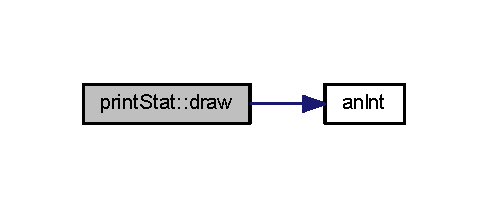
\includegraphics[width=234pt]{namespaceprint_stat_a07c0632a1accc08bdfc3990a9110e95b_cgraph}
\end{center}
\end{figure}




Here is the caller graph for this function\+:\nopagebreak
\begin{figure}[H]
\begin{center}
\leavevmode
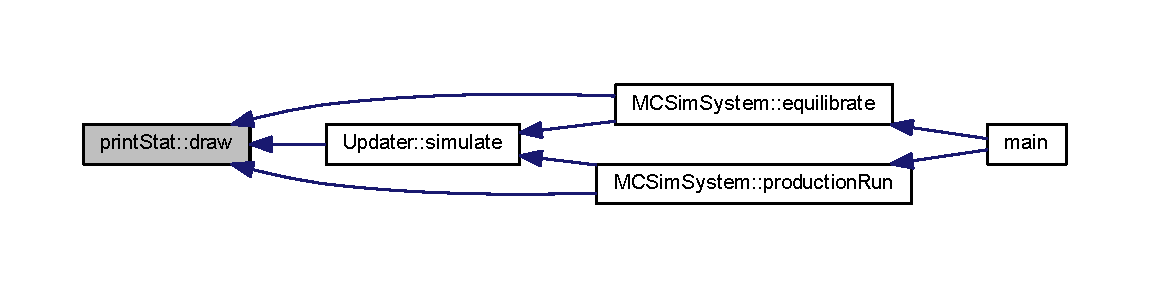
\includegraphics[width=350pt]{namespaceprint_stat_a07c0632a1accc08bdfc3990a9110e95b_icgraph}
\end{center}
\end{figure}


\hypertarget{namespaceprint_stat_a14daf62b11779bc1d5703953c7fe6c5e}{\index{print\+Stat@{print\+Stat}!print\+Cluster\+List@{print\+Cluster\+List}}
\index{print\+Cluster\+List@{print\+Cluster\+List}!print\+Stat@{print\+Stat}}
\subsubsection[{print\+Cluster\+List}]{\setlength{\rightskip}{0pt plus 5cm}int print\+Stat\+::print\+Cluster\+List (
\begin{DoxyParamCaption}
\item[{F\+I\+L\+E $\ast$}]{stream, }
\item[{bool}]{decor, }
\item[{{\bf Sim} $\ast$}]{sim, }
\item[{{\bf Conf} $\ast$}]{conf}
\end{DoxyParamCaption}
)}}\label{namespaceprint_stat_a14daf62b11779bc1d5703953c7fe6c5e}


print\+\_\+clusterlist print the clusterlist 


\begin{DoxyParams}{Parameters}
{\em stream} & \\
\hline
{\em decor} & \\
\hline
{\em topo} & \\
\hline
{\em sim} & \\
\hline
{\em conf} & \\
\hline
\end{DoxyParams}
\begin{DoxyReturn}{Returns}

\end{DoxyReturn}


Here is the caller graph for this function\+:\nopagebreak
\begin{figure}[H]
\begin{center}
\leavevmode
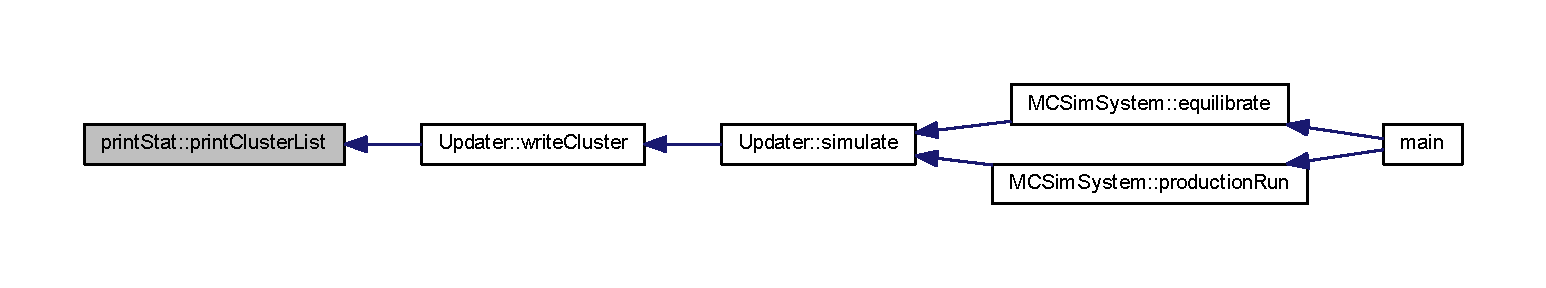
\includegraphics[width=350pt]{namespaceprint_stat_a14daf62b11779bc1d5703953c7fe6c5e_icgraph}
\end{center}
\end{figure}


\hypertarget{namespaceprint_stat_a677d67d06c5e94575cf134f62b8931ca}{\index{print\+Stat@{print\+Stat}!print\+Clusters@{print\+Clusters}}
\index{print\+Clusters@{print\+Clusters}!print\+Stat@{print\+Stat}}
\subsubsection[{print\+Clusters}]{\setlength{\rightskip}{0pt plus 5cm}int print\+Stat\+::print\+Clusters (
\begin{DoxyParamCaption}
\item[{F\+I\+L\+E $\ast$}]{stream, }
\item[{bool}]{decor, }
\item[{{\bf Sim} $\ast$}]{sim}
\end{DoxyParamCaption}
)}}\label{namespaceprint_stat_a677d67d06c5e94575cf134f62b8931ca}


print\+\_\+clusters print the clusters 


\begin{DoxyParams}{Parameters}
{\em stream} & \\
\hline
{\em decor} & \\
\hline
{\em sim} & \\
\hline
\end{DoxyParams}
\begin{DoxyReturn}{Returns}

\end{DoxyReturn}


Here is the caller graph for this function\+:\nopagebreak
\begin{figure}[H]
\begin{center}
\leavevmode
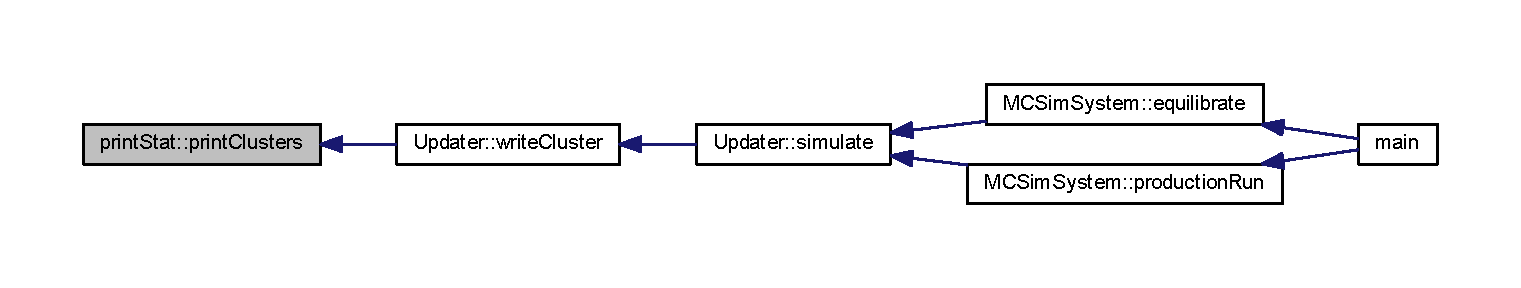
\includegraphics[width=350pt]{namespaceprint_stat_a677d67d06c5e94575cf134f62b8931ca_icgraph}
\end{center}
\end{figure}


\hypertarget{namespaceprint_stat_a0b43e80734258424961c75c73a97ad6c}{\index{print\+Stat@{print\+Stat}!print\+Cluster\+Stat@{print\+Cluster\+Stat}}
\index{print\+Cluster\+Stat@{print\+Cluster\+Stat}!print\+Stat@{print\+Stat}}
\subsubsection[{print\+Cluster\+Stat}]{\setlength{\rightskip}{0pt plus 5cm}int print\+Stat\+::print\+Cluster\+Stat (
\begin{DoxyParamCaption}
\item[{F\+I\+L\+E $\ast$}]{stream, }
\item[{bool}]{decor, }
\item[{{\bf Sim} $\ast$}]{sim}
\end{DoxyParamCaption}
)}}\label{namespaceprint_stat_a0b43e80734258424961c75c73a97ad6c}


print\+\_\+clusterstat print a statistics for the clusters 


\begin{DoxyParams}{Parameters}
{\em stream} & \\
\hline
{\em decor} & \\
\hline
{\em sim} & \\
\hline
\end{DoxyParams}
\begin{DoxyReturn}{Returns}

\end{DoxyReturn}


Here is the caller graph for this function\+:\nopagebreak
\begin{figure}[H]
\begin{center}
\leavevmode
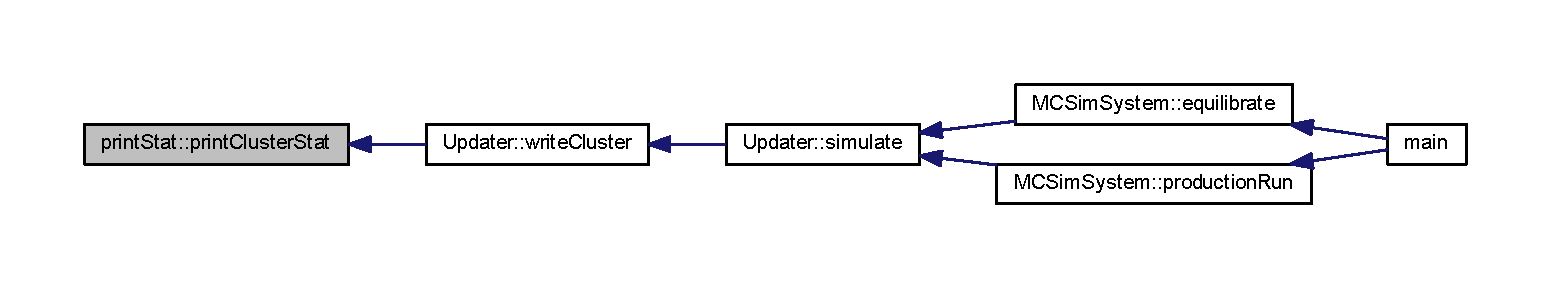
\includegraphics[width=350pt]{namespaceprint_stat_a0b43e80734258424961c75c73a97ad6c_icgraph}
\end{center}
\end{figure}


\hypertarget{namespaceprint_stat_a8170440b42d61f528a874c4d763609f7}{\index{print\+Stat@{print\+Stat}!print\+Eq\+Stat@{print\+Eq\+Stat}}
\index{print\+Eq\+Stat@{print\+Eq\+Stat}!print\+Stat@{print\+Stat}}
\subsubsection[{print\+Eq\+Stat}]{\setlength{\rightskip}{0pt plus 5cm}void print\+Stat\+::print\+Eq\+Stat (
\begin{DoxyParamCaption}
\item[{{\bf Disp} $\ast$}]{dat, }
\item[{double}]{scale, }
\item[{int}]{length}
\end{DoxyParamCaption}
)}}\label{namespaceprint_stat_a8170440b42d61f528a874c4d763609f7}


printeqstat 


\begin{DoxyParams}{Parameters}
{\em dat} & \\
\hline
{\em scale} & \\
\hline
{\em length} & \\
\hline
\end{DoxyParams}


Here is the caller graph for this function\+:\nopagebreak
\begin{figure}[H]
\begin{center}
\leavevmode
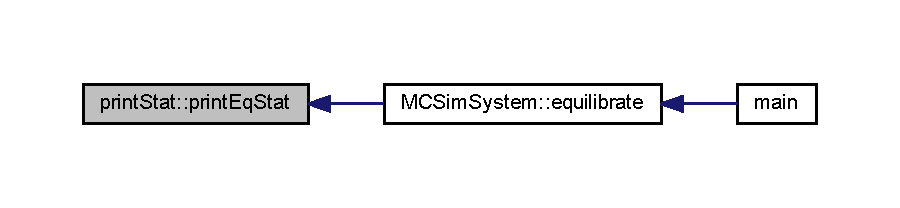
\includegraphics[width=350pt]{namespaceprint_stat_a8170440b42d61f528a874c4d763609f7_icgraph}
\end{center}
\end{figure}


\hypertarget{namespaceprint_stat_a323ee54f7e5beb4c642569cb07aa37ce}{\index{print\+Stat@{print\+Stat}!print\+Pair\+List@{print\+Pair\+List}}
\index{print\+Pair\+List@{print\+Pair\+List}!print\+Stat@{print\+Stat}}
\subsubsection[{print\+Pair\+List}]{\setlength{\rightskip}{0pt plus 5cm}void print\+Stat\+::print\+Pair\+List (
\begin{DoxyParamCaption}
\item[{F\+I\+L\+E $\ast$}]{stream, }
\item[{{\bf Conf} $\ast$}]{conf}
\end{DoxyParamCaption}
)}}\label{namespaceprint_stat_a323ee54f7e5beb4c642569cb07aa37ce}


print\+\_\+pairlist Print out the pairlist 


\begin{DoxyParams}{Parameters}
{\em stream} & \\
\hline
{\em sim} & \\
\hline
{\em topo} & \\
\hline
\end{DoxyParams}

\chapter{Class Documentation}
\hypertarget{struct_cluster}{\section{Cluster Struct Reference}
\label{struct_cluster}\index{Cluster@{Cluster}}
}


contains all the particles of one cluster  




{\ttfamily \#include $<$structures.\+h$>$}

\subsection*{Public Attributes}
\begin{DoxyCompactItemize}
\item 
long \hyperlink{struct_cluster_ade4bba0e66c1644effb8546ecf3bd6e3}{npart}
\item 
long $\ast$ \hyperlink{struct_cluster_a5a7b9b56c48051aba1bc45440c3b1e08}{particles}
\end{DoxyCompactItemize}


\subsection{Detailed Description}
contains all the particles of one cluster 

\subsection{Member Data Documentation}
\hypertarget{struct_cluster_ade4bba0e66c1644effb8546ecf3bd6e3}{\index{Cluster@{Cluster}!npart@{npart}}
\index{npart@{npart}!Cluster@{Cluster}}
\subsubsection[{npart}]{\setlength{\rightskip}{0pt plus 5cm}long Cluster\+::npart}}\label{struct_cluster_ade4bba0e66c1644effb8546ecf3bd6e3}
\hypertarget{struct_cluster_a5a7b9b56c48051aba1bc45440c3b1e08}{\index{Cluster@{Cluster}!particles@{particles}}
\index{particles@{particles}!Cluster@{Cluster}}
\subsubsection[{particles}]{\setlength{\rightskip}{0pt plus 5cm}long$\ast$ Cluster\+::particles}}\label{struct_cluster_a5a7b9b56c48051aba1bc45440c3b1e08}


The documentation for this struct was generated from the following file\+:\begin{DoxyCompactItemize}
\item 
sc\+O\+O\+P/structures/\hyperlink{structures_8h}{structures.\+h}\end{DoxyCompactItemize}

\hypertarget{class_conf}{\section{Conf Class Reference}
\label{class_conf}\index{Conf@{Conf}}
}


Configuration of the system.  




{\ttfamily \#include $<$Conf.\+h$>$}



Collaboration diagram for Conf\+:\nopagebreak
\begin{figure}[H]
\begin{center}
\leavevmode
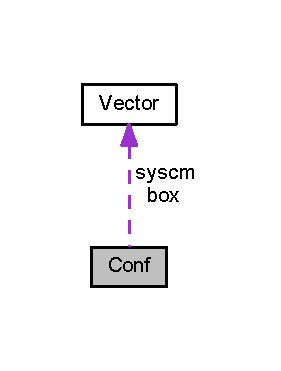
\includegraphics[width=135pt]{class_conf__coll__graph}
\end{center}
\end{figure}
\subsection*{Public Member Functions}
\begin{DoxyCompactItemize}
\item 
\hyperlink{class_conf_a143db233420f3d2ad3863c5320d6796d}{Conf} ()
\begin{DoxyCompactList}\small\item\em \hyperlink{class_conf}{Conf} Constructor, initializing variables. \end{DoxyCompactList}\item 
int \hyperlink{class_conf_a8b78f1efdb4d4d4f12c62eb390f791ad}{to\+Store\+Index} (int mol\+Type, int mol\+I\+D)
\begin{DoxyCompactList}\small\item\em Converts mol\+I\+D of mol\+Type to particle\+Store Index mol\+I\+D -\/$>$ starts from 0 for each mol\+Type. \end{DoxyCompactList}\item 
int \hyperlink{class_conf_a68e649d0ef31cb107f679598b0391f93}{mol\+Count\+Of\+Type} (int mol\+Type)
\item 
void \hyperlink{class_conf_a0fd2eec969a7e9c1024f02386abf1819}{add\+Molecule} (\hyperlink{class_particle}{Particle} $\ast$molecule)
\begin{DoxyCompactList}\small\item\em Adds molecule to particle\+Store, ensures \hyperlink{class_particle}{Particle} order, changes chainlist, grouplist. \end{DoxyCompactList}\item 
void \hyperlink{class_conf_a520317461ad1275019b00b58816e29b3}{remove\+Molecule} (int mol\+Type, int mol\+I\+D)
\begin{DoxyCompactList}\small\item\em remove\+Molecule \end{DoxyCompactList}\item 
void \hyperlink{class_conf_a4f70f2b18865d894c00fa0138247e32f}{mass\+Center} (\hyperlink{class_topo}{Topo} $\ast$topo)
\begin{DoxyCompactList}\small\item\em mass\+Center \end{DoxyCompactList}\item 
void \hyperlink{class_conf_ad1b87bd14eb659a88c59668c78b6bf02}{part\+Vec\+Init} (\hyperlink{class_topo}{Topo} $\ast$topo)
\begin{DoxyCompactList}\small\item\em partvecinit calculate vectors on particles for speedup \end{DoxyCompactList}\item 
int \hyperlink{class_conf_a5e8333ea6a4c8d4ef64f1b675aa61c66}{overlap} (\hyperlink{class_particle}{Particle} $\ast$part1, \hyperlink{class_particle}{Particle} $\ast$part2, \hyperlink{class_ia__param}{Ia\+\_\+param} ia\+\_\+params\mbox{[}\hyperlink{macros_8h_a3f79fdecc884eb98c97d1bdc77455295}{M\+A\+X\+T}\mbox{]}\mbox{[}\hyperlink{macros_8h_a3f79fdecc884eb98c97d1bdc77455295}{M\+A\+X\+T}\mbox{]})
\begin{DoxyCompactList}\small\item\em Determines whether two particles overlap. \end{DoxyCompactList}\item 
double \hyperlink{class_conf_a6e0faf2e313a9b5029d09b1d03523132}{linemin} (double criterion, double halfl)
\item 
bool \hyperlink{class_conf_a70be9b800e58ca0b8a70d8d82bb865b8}{overlap\+All} (\hyperlink{class_particle}{Particle} $\ast$target, \hyperlink{class_ia__param}{Ia\+\_\+param} ia\+\_\+params\mbox{[}\hyperlink{macros_8h_a3f79fdecc884eb98c97d1bdc77455295}{M\+A\+X\+T}\mbox{]}\mbox{[}\hyperlink{macros_8h_a3f79fdecc884eb98c97d1bdc77455295}{M\+A\+X\+T}\mbox{]})
\begin{DoxyCompactList}\small\item\em forbidden Checks for overlaps between particle \char`\"{}target\char`\"{} and the rest. \end{DoxyCompactList}\item 
int \hyperlink{class_conf_ad9286a65f6233e0f25b14a84e23e58b7}{checkall} (\hyperlink{class_ia__param}{Ia\+\_\+param} ia\+\_\+params\mbox{[}\hyperlink{macros_8h_a3f79fdecc884eb98c97d1bdc77455295}{M\+A\+X\+T}\mbox{]}\mbox{[}\hyperlink{macros_8h_a3f79fdecc884eb98c97d1bdc77455295}{M\+A\+X\+T}\mbox{]})
\begin{DoxyCompactList}\small\item\em checkall Checks for overlaps between all pairs of particles. \end{DoxyCompactList}\end{DoxyCompactItemize}
\subsection*{Public Attributes}
\begin{DoxyCompactItemize}
\item 
std\+::vector$<$ \hyperlink{class_particle}{Particle} $>$ \hyperlink{class_conf_a338d1f9d722924ef7bdf230cec6d8713}{particle\+Store}
\begin{DoxyCompactList}\small\item\em Main store of all particles, grouped by Molecular types. \end{DoxyCompactList}\item 
\hyperlink{class_vector}{Vector} \hyperlink{class_conf_a98e73199812404fd886619f90f0b26e7}{box}
\begin{DoxyCompactList}\small\item\em Box size $\ast$/. \end{DoxyCompactList}\item 
double \hyperlink{class_conf_a0591e720e4f06449a7d37a8e3135ddb1}{sysvolume}
\begin{DoxyCompactList}\small\item\em Something like total mass -\/$>$ for each += mass\+Of\+Particle. \end{DoxyCompactList}\item 
\hyperlink{class_vector}{Vector} \hyperlink{class_conf_a8d27bcc5bf535c39c7c0f17a078448d9}{syscm}
\begin{DoxyCompactList}\small\item\em System center of mass. \end{DoxyCompactList}\item 
int \hyperlink{class_conf_a907de4d9eb23d6480a16007c5087382c}{first} \mbox{[}\hyperlink{macros_8h_ad002a98462c90c52983b122ab9e2059a}{M\+A\+X\+M\+T}\mbox{]}
\begin{DoxyCompactList}\small\item\em Index(of particle\+Store) of first particle of molecule type, array over molecular types. \end{DoxyCompactList}\item 
int \hyperlink{class_conf_ae8941c30c3bdb0bb5bd33db013a60993}{mol\+Size} \mbox{[}\hyperlink{macros_8h_ad002a98462c90c52983b122ab9e2059a}{M\+A\+X\+M\+T}\mbox{]}
\begin{DoxyCompactList}\small\item\em Number of particles per molecule of molecule\+Type, array over molecular types. \end{DoxyCompactList}\item 
int \hyperlink{class_conf_a0eea95a1c34f8ace0939fd75eb7fe55f}{mol\+Type\+Count}
\begin{DoxyCompactList}\small\item\em Count of molecular types in use. \end{DoxyCompactList}\item 
long \hyperlink{class_conf_a8da63e8eb7fb59124bea9e082fa447eb}{chainlist} \mbox{[}\hyperlink{macros_8h_ad1f79d9d99776d7353c6659c307c83c6}{M\+A\+X\+N}\mbox{]}\mbox{[}\hyperlink{macros_8h_a6ba68031db49c489a6a5902f87b915c8}{M\+A\+X\+C\+H\+L}\mbox{]}
\begin{DoxyCompactList}\small\item\em List of particles in chain. \end{DoxyCompactList}\item 
long \hyperlink{class_conf_a9e62de59bb1879dc0653037155d045a9}{chain\+Count}
\begin{DoxyCompactList}\small\item\em Number of chains. \end{DoxyCompactList}\end{DoxyCompactItemize}


\subsection{Detailed Description}
Configuration of the system. 

\subsection{Constructor \& Destructor Documentation}
\hypertarget{class_conf_a143db233420f3d2ad3863c5320d6796d}{\index{Conf@{Conf}!Conf@{Conf}}
\index{Conf@{Conf}!Conf@{Conf}}
\subsubsection[{Conf}]{\setlength{\rightskip}{0pt plus 5cm}Conf\+::\+Conf (
\begin{DoxyParamCaption}
{}
\end{DoxyParamCaption}
)\hspace{0.3cm}{\ttfamily [inline]}}}\label{class_conf_a143db233420f3d2ad3863c5320d6796d}


\hyperlink{class_conf}{Conf} Constructor, initializing variables. 



\subsection{Member Function Documentation}
\hypertarget{class_conf_a0fd2eec969a7e9c1024f02386abf1819}{\index{Conf@{Conf}!add\+Molecule@{add\+Molecule}}
\index{add\+Molecule@{add\+Molecule}!Conf@{Conf}}
\subsubsection[{add\+Molecule}]{\setlength{\rightskip}{0pt plus 5cm}void Conf\+::add\+Molecule (
\begin{DoxyParamCaption}
\item[{{\bf Particle} $\ast$}]{molecule}
\end{DoxyParamCaption}
)}}\label{class_conf_a0fd2eec969a7e9c1024f02386abf1819}


Adds molecule to particle\+Store, ensures \hyperlink{class_particle}{Particle} order, changes chainlist, grouplist. 


\begin{DoxyParams}{Parameters}
{\em molecule} & \\
\hline
{\em topo} & \\
\hline
\end{DoxyParams}


Here is the caller graph for this function\+:
\nopagebreak
\begin{figure}[H]
\begin{center}
\leavevmode
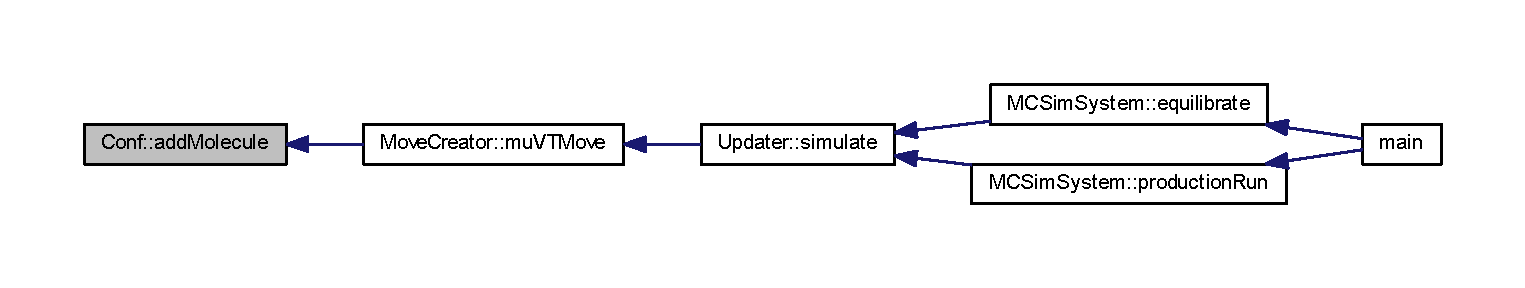
\includegraphics[width=350pt]{class_conf_a0fd2eec969a7e9c1024f02386abf1819_icgraph}
\end{center}
\end{figure}


\hypertarget{class_conf_ad9286a65f6233e0f25b14a84e23e58b7}{\index{Conf@{Conf}!checkall@{checkall}}
\index{checkall@{checkall}!Conf@{Conf}}
\subsubsection[{checkall}]{\setlength{\rightskip}{0pt plus 5cm}int Conf\+::checkall (
\begin{DoxyParamCaption}
\item[{{\bf Ia\+\_\+param}}]{ia\+\_\+params\mbox{[}\+M\+A\+X\+T\mbox{]}\mbox{[}\+M\+A\+X\+T\mbox{]}}
\end{DoxyParamCaption}
)}}\label{class_conf_ad9286a65f6233e0f25b14a84e23e58b7}


checkall Checks for overlaps between all pairs of particles. 


\begin{DoxyParams}{Parameters}
{\em ia\+\_\+params} & \\
\hline
\end{DoxyParams}
\begin{DoxyReturn}{Returns}
Returns 1 if overlap detected, 0 otherwise. 
\end{DoxyReturn}


Here is the call graph for this function\+:\nopagebreak
\begin{figure}[H]
\begin{center}
\leavevmode
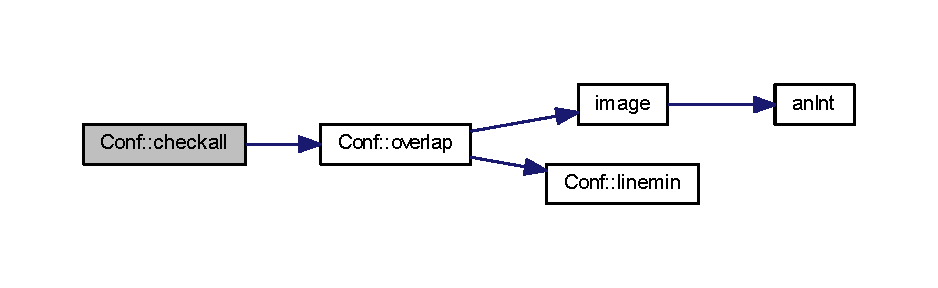
\includegraphics[width=350pt]{class_conf_ad9286a65f6233e0f25b14a84e23e58b7_cgraph}
\end{center}
\end{figure}


\hypertarget{class_conf_a6e0faf2e313a9b5029d09b1d03523132}{\index{Conf@{Conf}!linemin@{linemin}}
\index{linemin@{linemin}!Conf@{Conf}}
\subsubsection[{linemin}]{\setlength{\rightskip}{0pt plus 5cm}double Conf\+::linemin (
\begin{DoxyParamCaption}
\item[{double}]{criterion, }
\item[{double}]{halfl}
\end{DoxyParamCaption}
)\hspace{0.3cm}{\ttfamily [inline]}}}\label{class_conf_a6e0faf2e313a9b5029d09b1d03523132}


Here is the caller graph for this function\+:\nopagebreak
\begin{figure}[H]
\begin{center}
\leavevmode
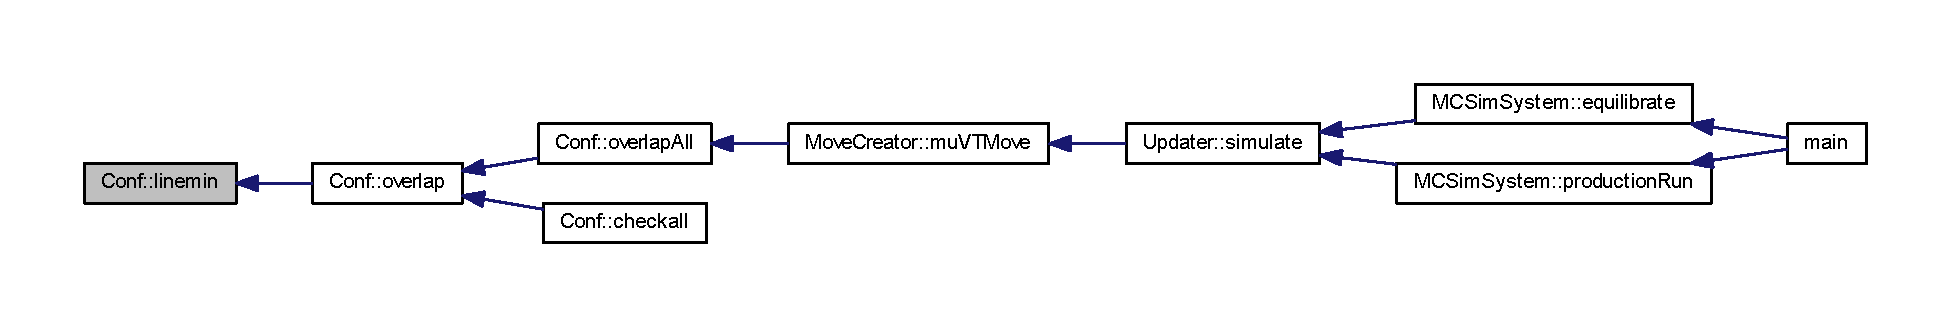
\includegraphics[width=350pt]{class_conf_a6e0faf2e313a9b5029d09b1d03523132_icgraph}
\end{center}
\end{figure}


\hypertarget{class_conf_a4f70f2b18865d894c00fa0138247e32f}{\index{Conf@{Conf}!mass\+Center@{mass\+Center}}
\index{mass\+Center@{mass\+Center}!Conf@{Conf}}
\subsubsection[{mass\+Center}]{\setlength{\rightskip}{0pt plus 5cm}void Conf\+::mass\+Center (
\begin{DoxyParamCaption}
\item[{{\bf Topo} $\ast$}]{topo}
\end{DoxyParamCaption}
)}}\label{class_conf_a4f70f2b18865d894c00fa0138247e32f}


mass\+Center 


\begin{DoxyParams}{Parameters}
{\em topo} & \\
\hline
\end{DoxyParams}


Here is the call graph for this function\+:\nopagebreak
\begin{figure}[H]
\begin{center}
\leavevmode
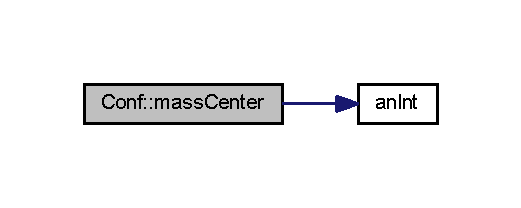
\includegraphics[width=250pt]{class_conf_a4f70f2b18865d894c00fa0138247e32f_cgraph}
\end{center}
\end{figure}




Here is the caller graph for this function\+:
\nopagebreak
\begin{figure}[H]
\begin{center}
\leavevmode
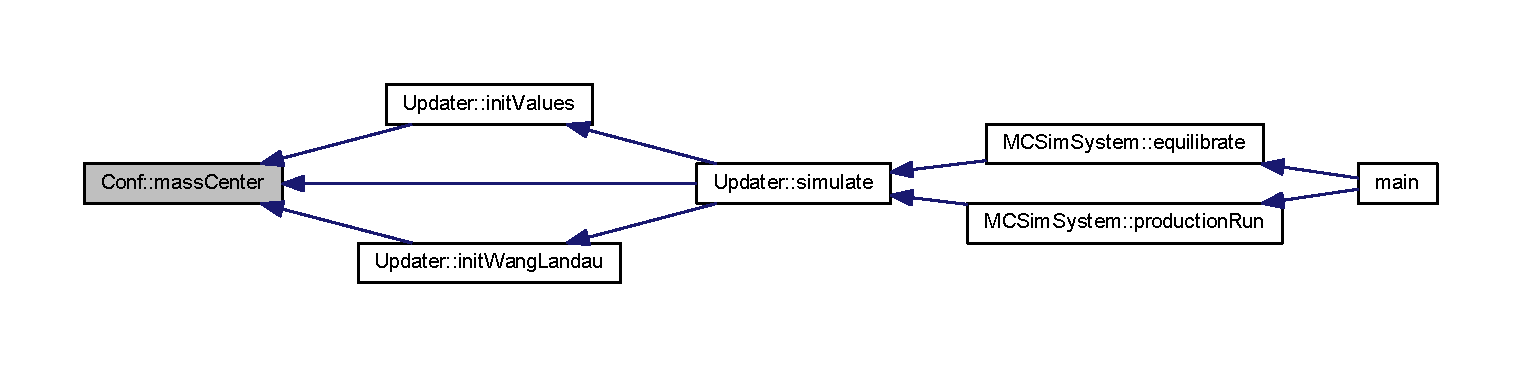
\includegraphics[width=350pt]{class_conf_a4f70f2b18865d894c00fa0138247e32f_icgraph}
\end{center}
\end{figure}


\hypertarget{class_conf_a68e649d0ef31cb107f679598b0391f93}{\index{Conf@{Conf}!mol\+Count\+Of\+Type@{mol\+Count\+Of\+Type}}
\index{mol\+Count\+Of\+Type@{mol\+Count\+Of\+Type}!Conf@{Conf}}
\subsubsection[{mol\+Count\+Of\+Type}]{\setlength{\rightskip}{0pt plus 5cm}int Conf\+::mol\+Count\+Of\+Type (
\begin{DoxyParamCaption}
\item[{int}]{mol\+Type}
\end{DoxyParamCaption}
)\hspace{0.3cm}{\ttfamily [inline]}}}\label{class_conf_a68e649d0ef31cb107f679598b0391f93}

\begin{DoxyParams}{Parameters}
{\em Type} & of molecule \\
\hline
\end{DoxyParams}
\begin{DoxyReturn}{Returns}
Number of molecules a given type 
\end{DoxyReturn}


Here is the caller graph for this function\+:
\nopagebreak
\begin{figure}[H]
\begin{center}
\leavevmode
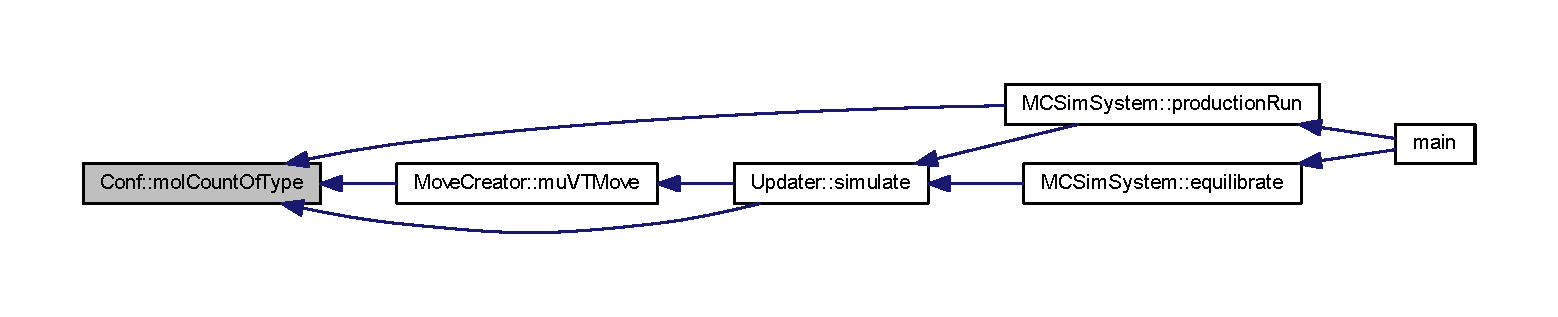
\includegraphics[width=350pt]{class_conf_a68e649d0ef31cb107f679598b0391f93_icgraph}
\end{center}
\end{figure}


\hypertarget{class_conf_a5e8333ea6a4c8d4ef64f1b675aa61c66}{\index{Conf@{Conf}!overlap@{overlap}}
\index{overlap@{overlap}!Conf@{Conf}}
\subsubsection[{overlap}]{\setlength{\rightskip}{0pt plus 5cm}int Conf\+::overlap (
\begin{DoxyParamCaption}
\item[{{\bf Particle} $\ast$}]{part1, }
\item[{{\bf Particle} $\ast$}]{part2, }
\item[{{\bf Ia\+\_\+param}}]{ia\+\_\+params\mbox{[}\+M\+A\+X\+T\mbox{]}\mbox{[}\+M\+A\+X\+T\mbox{]}}
\end{DoxyParamCaption}
)}}\label{class_conf_a5e8333ea6a4c8d4ef64f1b675aa61c66}


Determines whether two particles overlap. 


\begin{DoxyParams}{Parameters}
{\em part1} & \\
\hline
{\em part2} & \\
\hline
{\em ia\+\_\+params} & 1 if there is an overlap, 0 if not. \\
\hline
\end{DoxyParams}
\begin{DoxyReturn}{Returns}

\end{DoxyReturn}


Here is the call graph for this function\+:\nopagebreak
\begin{figure}[H]
\begin{center}
\leavevmode
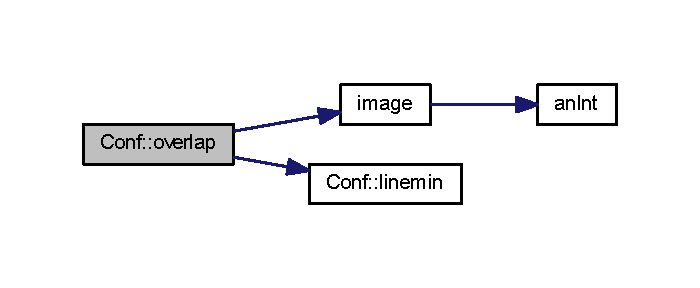
\includegraphics[width=336pt]{class_conf_a5e8333ea6a4c8d4ef64f1b675aa61c66_cgraph}
\end{center}
\end{figure}




Here is the caller graph for this function\+:\nopagebreak
\begin{figure}[H]
\begin{center}
\leavevmode
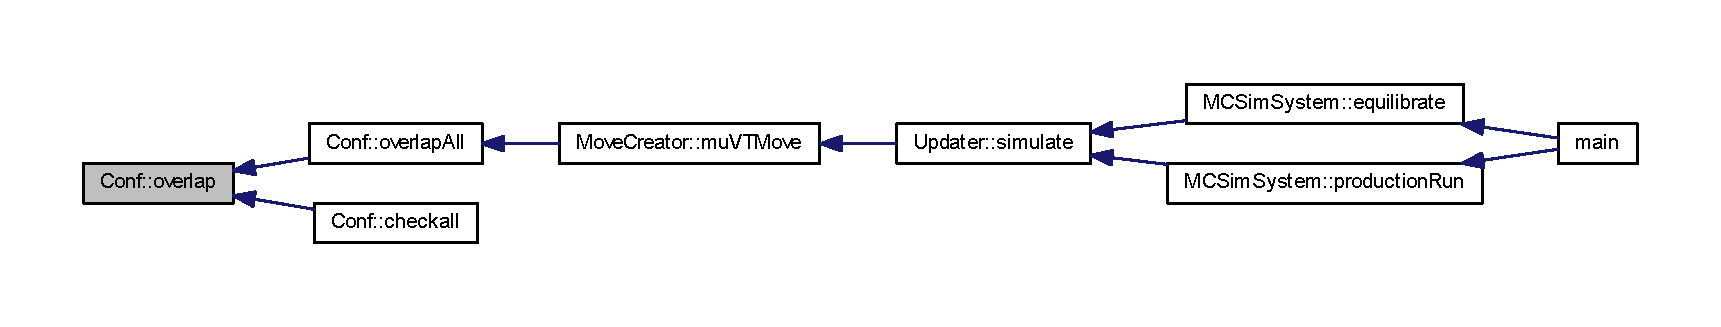
\includegraphics[width=350pt]{class_conf_a5e8333ea6a4c8d4ef64f1b675aa61c66_icgraph}
\end{center}
\end{figure}


\hypertarget{class_conf_a70be9b800e58ca0b8a70d8d82bb865b8}{\index{Conf@{Conf}!overlap\+All@{overlap\+All}}
\index{overlap\+All@{overlap\+All}!Conf@{Conf}}
\subsubsection[{overlap\+All}]{\setlength{\rightskip}{0pt plus 5cm}bool Conf\+::overlap\+All (
\begin{DoxyParamCaption}
\item[{{\bf Particle} $\ast$}]{target, }
\item[{{\bf Ia\+\_\+param}}]{ia\+\_\+params\mbox{[}\+M\+A\+X\+T\mbox{]}\mbox{[}\+M\+A\+X\+T\mbox{]}}
\end{DoxyParamCaption}
)}}\label{class_conf_a70be9b800e58ca0b8a70d8d82bb865b8}


forbidden Checks for overlaps between particle \char`\"{}target\char`\"{} and the rest. 


\begin{DoxyParams}{Parameters}
{\em target} & \\
\hline
{\em ia\+\_\+params} & \\
\hline
\end{DoxyParams}
\begin{DoxyReturn}{Returns}
Returns true if overlap detected, false otherwise. 
\end{DoxyReturn}


Here is the call graph for this function\+:\nopagebreak
\begin{figure}[H]
\begin{center}
\leavevmode
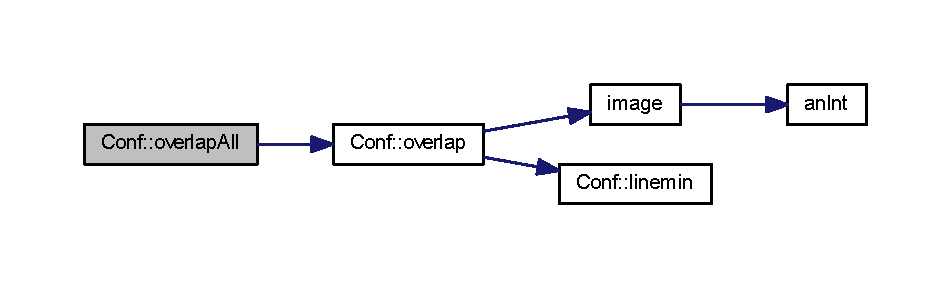
\includegraphics[width=350pt]{class_conf_a70be9b800e58ca0b8a70d8d82bb865b8_cgraph}
\end{center}
\end{figure}




Here is the caller graph for this function\+:\nopagebreak
\begin{figure}[H]
\begin{center}
\leavevmode
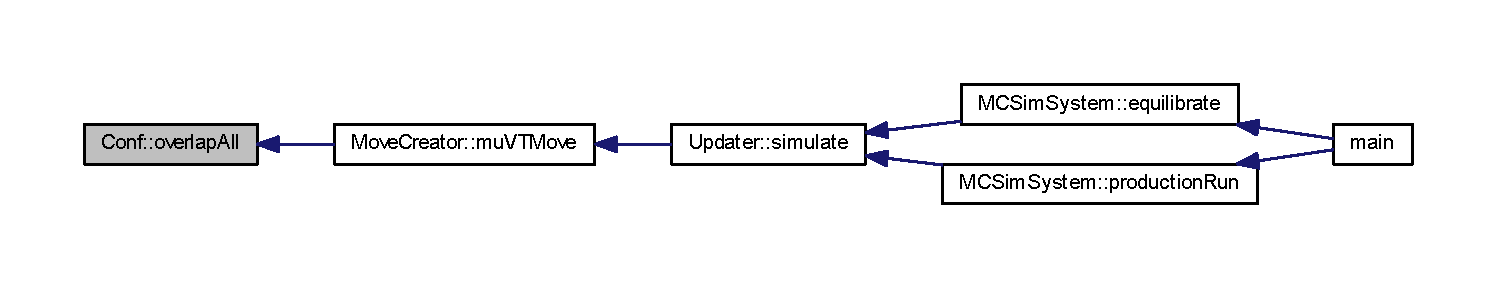
\includegraphics[width=350pt]{class_conf_a70be9b800e58ca0b8a70d8d82bb865b8_icgraph}
\end{center}
\end{figure}


\hypertarget{class_conf_ad1b87bd14eb659a88c59668c78b6bf02}{\index{Conf@{Conf}!part\+Vec\+Init@{part\+Vec\+Init}}
\index{part\+Vec\+Init@{part\+Vec\+Init}!Conf@{Conf}}
\subsubsection[{part\+Vec\+Init}]{\setlength{\rightskip}{0pt plus 5cm}void Conf\+::part\+Vec\+Init (
\begin{DoxyParamCaption}
\item[{{\bf Topo} $\ast$}]{topo}
\end{DoxyParamCaption}
)}}\label{class_conf_ad1b87bd14eb659a88c59668c78b6bf02}


partvecinit calculate vectors on particles for speedup 



Here is the caller graph for this function\+:
\nopagebreak
\begin{figure}[H]
\begin{center}
\leavevmode
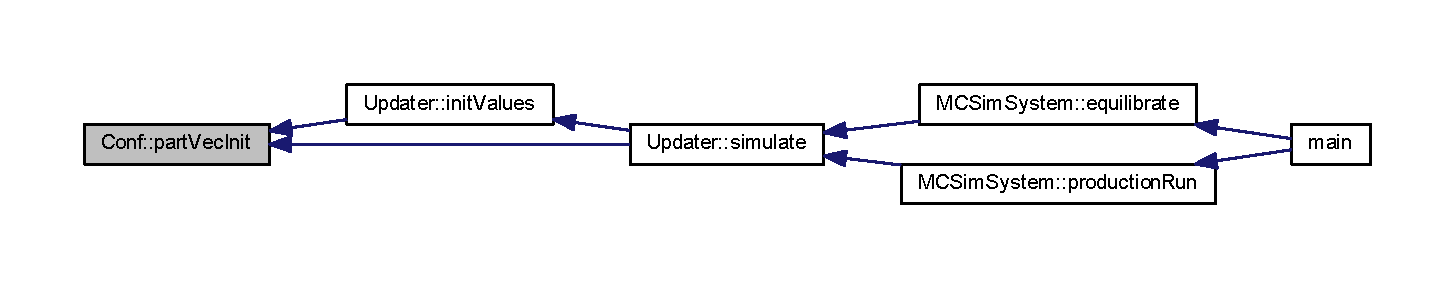
\includegraphics[width=350pt]{class_conf_ad1b87bd14eb659a88c59668c78b6bf02_icgraph}
\end{center}
\end{figure}


\hypertarget{class_conf_a520317461ad1275019b00b58816e29b3}{\index{Conf@{Conf}!remove\+Molecule@{remove\+Molecule}}
\index{remove\+Molecule@{remove\+Molecule}!Conf@{Conf}}
\subsubsection[{remove\+Molecule}]{\setlength{\rightskip}{0pt plus 5cm}void Conf\+::remove\+Molecule (
\begin{DoxyParamCaption}
\item[{int}]{mol\+Type, }
\item[{int}]{mol\+I\+D}
\end{DoxyParamCaption}
)}}\label{class_conf_a520317461ad1275019b00b58816e29b3}


remove\+Molecule 


\begin{DoxyParams}{Parameters}
{\em mol\+Type} & \\
\hline
{\em mol\+I\+D} & \\
\hline
\end{DoxyParams}


Here is the call graph for this function\+:
\nopagebreak
\begin{figure}[H]
\begin{center}
\leavevmode
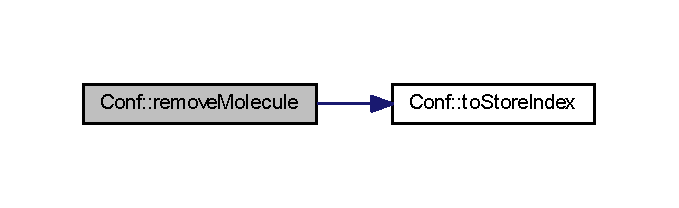
\includegraphics[width=326pt]{class_conf_a520317461ad1275019b00b58816e29b3_cgraph}
\end{center}
\end{figure}




Here is the caller graph for this function\+:
\nopagebreak
\begin{figure}[H]
\begin{center}
\leavevmode
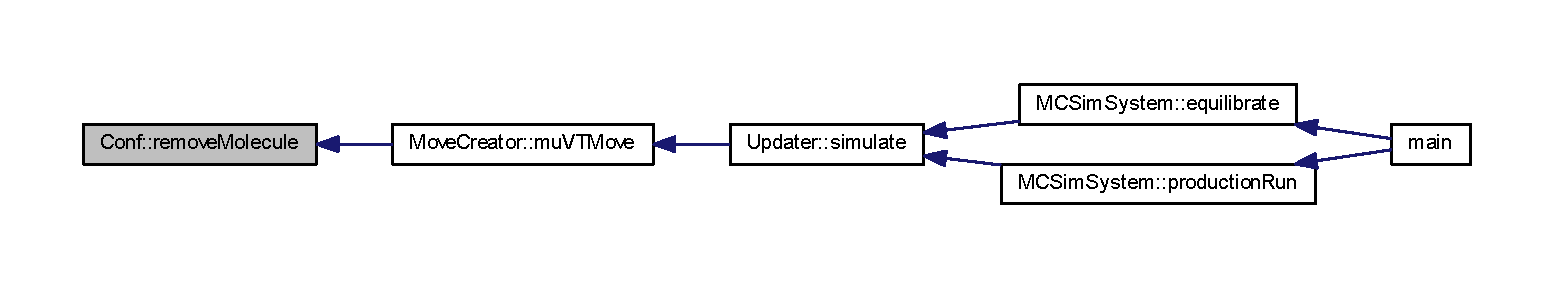
\includegraphics[width=350pt]{class_conf_a520317461ad1275019b00b58816e29b3_icgraph}
\end{center}
\end{figure}


\hypertarget{class_conf_a8b78f1efdb4d4d4f12c62eb390f791ad}{\index{Conf@{Conf}!to\+Store\+Index@{to\+Store\+Index}}
\index{to\+Store\+Index@{to\+Store\+Index}!Conf@{Conf}}
\subsubsection[{to\+Store\+Index}]{\setlength{\rightskip}{0pt plus 5cm}int Conf\+::to\+Store\+Index (
\begin{DoxyParamCaption}
\item[{int}]{mol\+Type, }
\item[{int}]{mol\+I\+D}
\end{DoxyParamCaption}
)\hspace{0.3cm}{\ttfamily [inline]}}}\label{class_conf_a8b78f1efdb4d4d4f12c62eb390f791ad}


Converts mol\+I\+D of mol\+Type to particle\+Store Index mol\+I\+D -\/$>$ starts from 0 for each mol\+Type. 

\begin{DoxyReturn}{Returns}
Index of first particle of molecule 
\end{DoxyReturn}


Here is the caller graph for this function\+:
\nopagebreak
\begin{figure}[H]
\begin{center}
\leavevmode
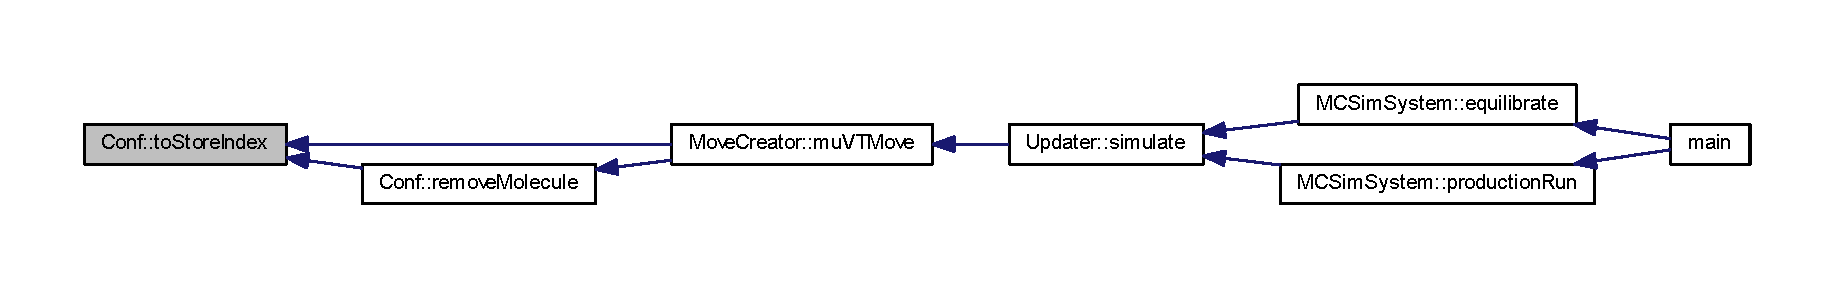
\includegraphics[width=350pt]{class_conf_a8b78f1efdb4d4d4f12c62eb390f791ad_icgraph}
\end{center}
\end{figure}




\subsection{Member Data Documentation}
\hypertarget{class_conf_a98e73199812404fd886619f90f0b26e7}{\index{Conf@{Conf}!box@{box}}
\index{box@{box}!Conf@{Conf}}
\subsubsection[{box}]{\setlength{\rightskip}{0pt plus 5cm}{\bf Vector} Conf\+::box}}\label{class_conf_a98e73199812404fd886619f90f0b26e7}


Box size $\ast$/. 

\hypertarget{class_conf_a9e62de59bb1879dc0653037155d045a9}{\index{Conf@{Conf}!chain\+Count@{chain\+Count}}
\index{chain\+Count@{chain\+Count}!Conf@{Conf}}
\subsubsection[{chain\+Count}]{\setlength{\rightskip}{0pt plus 5cm}long Conf\+::chain\+Count}}\label{class_conf_a9e62de59bb1879dc0653037155d045a9}


Number of chains. 

\hypertarget{class_conf_a8da63e8eb7fb59124bea9e082fa447eb}{\index{Conf@{Conf}!chainlist@{chainlist}}
\index{chainlist@{chainlist}!Conf@{Conf}}
\subsubsection[{chainlist}]{\setlength{\rightskip}{0pt plus 5cm}long Conf\+::chainlist\mbox{[}{\bf M\+A\+X\+N}\mbox{]}\mbox{[}{\bf M\+A\+X\+C\+H\+L}\mbox{]}}}\label{class_conf_a8da63e8eb7fb59124bea9e082fa447eb}


List of particles in chain. 

\hypertarget{class_conf_a907de4d9eb23d6480a16007c5087382c}{\index{Conf@{Conf}!first@{first}}
\index{first@{first}!Conf@{Conf}}
\subsubsection[{first}]{\setlength{\rightskip}{0pt plus 5cm}int Conf\+::first\mbox{[}{\bf M\+A\+X\+M\+T}\mbox{]}}}\label{class_conf_a907de4d9eb23d6480a16007c5087382c}


Index(of particle\+Store) of first particle of molecule type, array over molecular types. 

\hypertarget{class_conf_ae8941c30c3bdb0bb5bd33db013a60993}{\index{Conf@{Conf}!mol\+Size@{mol\+Size}}
\index{mol\+Size@{mol\+Size}!Conf@{Conf}}
\subsubsection[{mol\+Size}]{\setlength{\rightskip}{0pt plus 5cm}int Conf\+::mol\+Size\mbox{[}{\bf M\+A\+X\+M\+T}\mbox{]}}}\label{class_conf_ae8941c30c3bdb0bb5bd33db013a60993}


Number of particles per molecule of molecule\+Type, array over molecular types. 

\hypertarget{class_conf_a0eea95a1c34f8ace0939fd75eb7fe55f}{\index{Conf@{Conf}!mol\+Type\+Count@{mol\+Type\+Count}}
\index{mol\+Type\+Count@{mol\+Type\+Count}!Conf@{Conf}}
\subsubsection[{mol\+Type\+Count}]{\setlength{\rightskip}{0pt plus 5cm}int Conf\+::mol\+Type\+Count}}\label{class_conf_a0eea95a1c34f8ace0939fd75eb7fe55f}


Count of molecular types in use. 

\hypertarget{class_conf_a338d1f9d722924ef7bdf230cec6d8713}{\index{Conf@{Conf}!particle\+Store@{particle\+Store}}
\index{particle\+Store@{particle\+Store}!Conf@{Conf}}
\subsubsection[{particle\+Store}]{\setlength{\rightskip}{0pt plus 5cm}std\+::vector$<${\bf Particle} $>$ Conf\+::particle\+Store}}\label{class_conf_a338d1f9d722924ef7bdf230cec6d8713}


Main store of all particles, grouped by Molecular types. 

\hypertarget{class_conf_a8d27bcc5bf535c39c7c0f17a078448d9}{\index{Conf@{Conf}!syscm@{syscm}}
\index{syscm@{syscm}!Conf@{Conf}}
\subsubsection[{syscm}]{\setlength{\rightskip}{0pt plus 5cm}{\bf Vector} Conf\+::syscm}}\label{class_conf_a8d27bcc5bf535c39c7c0f17a078448d9}


System center of mass. 

\hypertarget{class_conf_a0591e720e4f06449a7d37a8e3135ddb1}{\index{Conf@{Conf}!sysvolume@{sysvolume}}
\index{sysvolume@{sysvolume}!Conf@{Conf}}
\subsubsection[{sysvolume}]{\setlength{\rightskip}{0pt plus 5cm}double Conf\+::sysvolume}}\label{class_conf_a0591e720e4f06449a7d37a8e3135ddb1}


Something like total mass -\/$>$ for each += mass\+Of\+Particle. 



The documentation for this class was generated from the following files\+:\begin{DoxyCompactItemize}
\item 
sc\+O\+O\+P/structures/\hyperlink{_conf_8h}{Conf.\+h}\item 
sc\+O\+O\+P/structures/\hyperlink{_conf_8cpp}{Conf.\+cpp}\end{DoxyCompactItemize}

\hypertarget{class_disp}{\section{Disp Class Reference}
\label{class_disp}\index{Disp@{Disp}}
}


Define step size and acceptance ratio statistics.  




{\ttfamily \#include $<$structures.\+h$>$}

\subsection*{Public Member Functions}
\begin{DoxyCompactItemize}
\item 
\hyperlink{class_disp_a9e3457b8cfea7679b70bd7e724134661}{Disp} ()
\end{DoxyCompactItemize}
\subsection*{Public Attributes}
\begin{DoxyCompactItemize}
\item 
double \hyperlink{class_disp_a12da7c0801e5ce844e28b7a785b7556c}{mx}
\begin{DoxyCompactList}\small\item\em Maximum value displacement, cos(angle), etc. \end{DoxyCompactList}\item 
double \hyperlink{class_disp_a40442346e379ba0674a8401502551b3a}{angle}
\begin{DoxyCompactList}\small\item\em Maximum angle, since in .mx cos(angle) is saved. \end{DoxyCompactList}\item 
long \hyperlink{class_disp_a2f55a3f871df675bd8eedbaa706b4c03}{acc}
\begin{DoxyCompactList}\small\item\em Number of accepted steps. \end{DoxyCompactList}\item 
long \hyperlink{class_disp_adcb197b8efb6392c5d08e1222cd488ee}{rej}
\begin{DoxyCompactList}\small\item\em Number of rejected steps. \end{DoxyCompactList}\item 
double \hyperlink{class_disp_ad895f0ec10cdd0f00de4a65667566f5b}{oldrmsd}
\begin{DoxyCompactList}\small\item\em Averaged mx value in previous equilibration round. \end{DoxyCompactList}\item 
double \hyperlink{class_disp_a3aa81c561f1dac48d4c486468b960919}{oldmx}
\begin{DoxyCompactList}\small\item\em Change in mx in last equlibrium step. \end{DoxyCompactList}\end{DoxyCompactItemize}


\subsection{Detailed Description}
Define step size and acceptance ratio statistics. 

\subsection{Constructor \& Destructor Documentation}
\hypertarget{class_disp_a9e3457b8cfea7679b70bd7e724134661}{\index{Disp@{Disp}!Disp@{Disp}}
\index{Disp@{Disp}!Disp@{Disp}}
\subsubsection[{Disp}]{\setlength{\rightskip}{0pt plus 5cm}Disp\+::\+Disp (
\begin{DoxyParamCaption}
{}
\end{DoxyParamCaption}
)\hspace{0.3cm}{\ttfamily [inline]}}}\label{class_disp_a9e3457b8cfea7679b70bd7e724134661}


\subsection{Member Data Documentation}
\hypertarget{class_disp_a2f55a3f871df675bd8eedbaa706b4c03}{\index{Disp@{Disp}!acc@{acc}}
\index{acc@{acc}!Disp@{Disp}}
\subsubsection[{acc}]{\setlength{\rightskip}{0pt plus 5cm}long Disp\+::acc}}\label{class_disp_a2f55a3f871df675bd8eedbaa706b4c03}


Number of accepted steps. 

\hypertarget{class_disp_a40442346e379ba0674a8401502551b3a}{\index{Disp@{Disp}!angle@{angle}}
\index{angle@{angle}!Disp@{Disp}}
\subsubsection[{angle}]{\setlength{\rightskip}{0pt plus 5cm}double Disp\+::angle}}\label{class_disp_a40442346e379ba0674a8401502551b3a}


Maximum angle, since in .mx cos(angle) is saved. 

\hypertarget{class_disp_a12da7c0801e5ce844e28b7a785b7556c}{\index{Disp@{Disp}!mx@{mx}}
\index{mx@{mx}!Disp@{Disp}}
\subsubsection[{mx}]{\setlength{\rightskip}{0pt plus 5cm}double Disp\+::mx}}\label{class_disp_a12da7c0801e5ce844e28b7a785b7556c}


Maximum value displacement, cos(angle), etc. 

\hypertarget{class_disp_a3aa81c561f1dac48d4c486468b960919}{\index{Disp@{Disp}!oldmx@{oldmx}}
\index{oldmx@{oldmx}!Disp@{Disp}}
\subsubsection[{oldmx}]{\setlength{\rightskip}{0pt plus 5cm}double Disp\+::oldmx}}\label{class_disp_a3aa81c561f1dac48d4c486468b960919}


Change in mx in last equlibrium step. 

\hypertarget{class_disp_ad895f0ec10cdd0f00de4a65667566f5b}{\index{Disp@{Disp}!oldrmsd@{oldrmsd}}
\index{oldrmsd@{oldrmsd}!Disp@{Disp}}
\subsubsection[{oldrmsd}]{\setlength{\rightskip}{0pt plus 5cm}double Disp\+::oldrmsd}}\label{class_disp_ad895f0ec10cdd0f00de4a65667566f5b}


Averaged mx value in previous equilibration round. 

\hypertarget{class_disp_adcb197b8efb6392c5d08e1222cd488ee}{\index{Disp@{Disp}!rej@{rej}}
\index{rej@{rej}!Disp@{Disp}}
\subsubsection[{rej}]{\setlength{\rightskip}{0pt plus 5cm}long Disp\+::rej}}\label{class_disp_adcb197b8efb6392c5d08e1222cd488ee}


Number of rejected steps. 



The documentation for this class was generated from the following file\+:\begin{DoxyCompactItemize}
\item 
sc\+O\+O\+P/structures/\hyperlink{structures_8h}{structures.\+h}\end{DoxyCompactItemize}

\hypertarget{class_exters}{\section{Exters Class Reference}
\label{class_exters}\index{Exters@{Exters}}
}


{\ttfamily \#include $<$structures.\+h$>$}



Collaboration diagram for Exters\+:\nopagebreak
\begin{figure}[H]
\begin{center}
\leavevmode
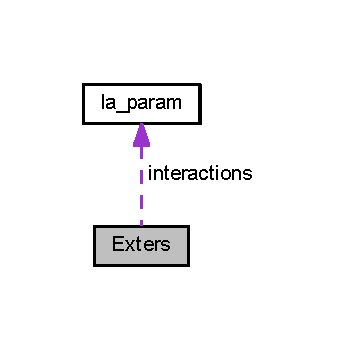
\includegraphics[width=162pt]{class_exters__coll__graph}
\end{center}
\end{figure}
\subsection*{Public Member Functions}
\begin{DoxyCompactItemize}
\item 
\hyperlink{class_exters_a36dd0bbb6aab1778f243d12e61aa0ad9}{Exters} ()
\end{DoxyCompactItemize}
\subsection*{Public Attributes}
\begin{DoxyCompactItemize}
\item 
bool \hyperlink{class_exters_a78d759bd9da50ad5c4669dae9c6172ff}{exist}
\begin{DoxyCompactList}\small\item\em existence of external potential \end{DoxyCompactList}\item 
double \hyperlink{class_exters_a6ac0235fe365f41ca035957b748c9564}{thickness}
\begin{DoxyCompactList}\small\item\em external wall thicnkess \end{DoxyCompactList}\item 
double \hyperlink{class_exters_ac6920553910e27bde3188120889e8381}{epsilon}
\begin{DoxyCompactList}\small\item\em depth of attraction \end{DoxyCompactList}\item 
double \hyperlink{class_exters_a3ace0154ce9823eaafe3e7d7c0ae71bc}{attraction}
\begin{DoxyCompactList}\small\item\em distance of attraction \end{DoxyCompactList}\item 
double \hyperlink{class_exters_ae4e012e33e40f87ef88b08072bdf2d07}{sqmaxcut}
\begin{DoxyCompactList}\small\item\em distance when nothing can interact \end{DoxyCompactList}\item 
\hyperlink{class_ia__param}{Ia\+\_\+param} \hyperlink{class_exters_adecb24b99a4014cd45182172733493b7}{interactions} \mbox{[}\hyperlink{macros_8h_a3f79fdecc884eb98c97d1bdc77455295}{M\+A\+X\+T}\mbox{]}
\begin{DoxyCompactList}\small\item\em Interaction parameters with particle types generated from above params. \end{DoxyCompactList}\end{DoxyCompactItemize}


\subsection{Constructor \& Destructor Documentation}
\hypertarget{class_exters_a36dd0bbb6aab1778f243d12e61aa0ad9}{\index{Exters@{Exters}!Exters@{Exters}}
\index{Exters@{Exters}!Exters@{Exters}}
\subsubsection[{Exters}]{\setlength{\rightskip}{0pt plus 5cm}Exters\+::\+Exters (
\begin{DoxyParamCaption}
{}
\end{DoxyParamCaption}
)\hspace{0.3cm}{\ttfamily [inline]}}}\label{class_exters_a36dd0bbb6aab1778f243d12e61aa0ad9}


\subsection{Member Data Documentation}
\hypertarget{class_exters_a3ace0154ce9823eaafe3e7d7c0ae71bc}{\index{Exters@{Exters}!attraction@{attraction}}
\index{attraction@{attraction}!Exters@{Exters}}
\subsubsection[{attraction}]{\setlength{\rightskip}{0pt plus 5cm}double Exters\+::attraction}}\label{class_exters_a3ace0154ce9823eaafe3e7d7c0ae71bc}


distance of attraction 

\hypertarget{class_exters_ac6920553910e27bde3188120889e8381}{\index{Exters@{Exters}!epsilon@{epsilon}}
\index{epsilon@{epsilon}!Exters@{Exters}}
\subsubsection[{epsilon}]{\setlength{\rightskip}{0pt plus 5cm}double Exters\+::epsilon}}\label{class_exters_ac6920553910e27bde3188120889e8381}


depth of attraction 

\hypertarget{class_exters_a78d759bd9da50ad5c4669dae9c6172ff}{\index{Exters@{Exters}!exist@{exist}}
\index{exist@{exist}!Exters@{Exters}}
\subsubsection[{exist}]{\setlength{\rightskip}{0pt plus 5cm}bool Exters\+::exist}}\label{class_exters_a78d759bd9da50ad5c4669dae9c6172ff}


existence of external potential 

\hypertarget{class_exters_adecb24b99a4014cd45182172733493b7}{\index{Exters@{Exters}!interactions@{interactions}}
\index{interactions@{interactions}!Exters@{Exters}}
\subsubsection[{interactions}]{\setlength{\rightskip}{0pt plus 5cm}{\bf Ia\+\_\+param} Exters\+::interactions\mbox{[}{\bf M\+A\+X\+T}\mbox{]}}}\label{class_exters_adecb24b99a4014cd45182172733493b7}


Interaction parameters with particle types generated from above params. 

\hypertarget{class_exters_ae4e012e33e40f87ef88b08072bdf2d07}{\index{Exters@{Exters}!sqmaxcut@{sqmaxcut}}
\index{sqmaxcut@{sqmaxcut}!Exters@{Exters}}
\subsubsection[{sqmaxcut}]{\setlength{\rightskip}{0pt plus 5cm}double Exters\+::sqmaxcut}}\label{class_exters_ae4e012e33e40f87ef88b08072bdf2d07}


distance when nothing can interact 

\hypertarget{class_exters_a6ac0235fe365f41ca035957b748c9564}{\index{Exters@{Exters}!thickness@{thickness}}
\index{thickness@{thickness}!Exters@{Exters}}
\subsubsection[{thickness}]{\setlength{\rightskip}{0pt plus 5cm}double Exters\+::thickness}}\label{class_exters_a6ac0235fe365f41ca035957b748c9564}


external wall thicnkess 



The documentation for this class was generated from the following file\+:\begin{DoxyCompactItemize}
\item 
sc\+O\+O\+P/structures/\hyperlink{structures_8h}{structures.\+h}\end{DoxyCompactItemize}

\hypertarget{struct_file_names}{\section{File\+Names Struct Reference}
\label{struct_file_names}\index{File\+Names@{File\+Names}}
}


{\ttfamily \#include $<$structures.\+h$>$}

\subsection*{Public Attributes}
\begin{DoxyCompactItemize}
\item 
char \hyperlink{struct_file_names_a2ba488883859beebf0e45d4fe64dce1e}{configurationinfile} \mbox{[}30\mbox{]}
\item 
char \hyperlink{struct_file_names_a5d57cf5a04876391b131a9c9307bc7d5}{topologyfile} \mbox{[}30\mbox{]}
\item 
char \hyperlink{struct_file_names_aef0ce496bdcc9b924a111438a1e16573}{optionsfile} \mbox{[}30\mbox{]}
\item 
char \hyperlink{struct_file_names_af41fd595b79047dfee97d3a66aa7ef40}{wlinfile} \mbox{[}30\mbox{]}
\item 
char \hyperlink{struct_file_names_a6d96709d8d21f5194c072ef80db0e8a7}{configurationoutfile} \mbox{[}30\mbox{]}
\item 
char \hyperlink{struct_file_names_ab6920a417c86a04aa771c248f75c6bf9}{moviefile} \mbox{[}30\mbox{]}
\item 
char \hyperlink{struct_file_names_ad3186b4b1d3a03d1cce61385475df1a9}{wloutfile} \mbox{[}30\mbox{]}
\item 
char \hyperlink{struct_file_names_a571bce947227b34ce9056cbff89c02b3}{statfile} \mbox{[}30\mbox{]}
\item 
char \hyperlink{struct_file_names_a308f1e0e953456ba44b873a1a336d707}{clusterfile} \mbox{[}30\mbox{]}
\item 
char \hyperlink{struct_file_names_a531ef786f58d7d412c6f841dd252e906}{clusterstatfile} \mbox{[}30\mbox{]}
\item 
char \hyperlink{struct_file_names_aab15a15f40bcf78ab8e6a00da44bc672}{energyfile} \mbox{[}30\mbox{]}
\end{DoxyCompactItemize}


\subsection{Member Data Documentation}
\hypertarget{struct_file_names_a308f1e0e953456ba44b873a1a336d707}{\index{File\+Names@{File\+Names}!clusterfile@{clusterfile}}
\index{clusterfile@{clusterfile}!File\+Names@{File\+Names}}
\subsubsection[{clusterfile}]{\setlength{\rightskip}{0pt plus 5cm}char File\+Names\+::clusterfile\mbox{[}30\mbox{]}}}\label{struct_file_names_a308f1e0e953456ba44b873a1a336d707}
\hypertarget{struct_file_names_a531ef786f58d7d412c6f841dd252e906}{\index{File\+Names@{File\+Names}!clusterstatfile@{clusterstatfile}}
\index{clusterstatfile@{clusterstatfile}!File\+Names@{File\+Names}}
\subsubsection[{clusterstatfile}]{\setlength{\rightskip}{0pt plus 5cm}char File\+Names\+::clusterstatfile\mbox{[}30\mbox{]}}}\label{struct_file_names_a531ef786f58d7d412c6f841dd252e906}
\hypertarget{struct_file_names_a2ba488883859beebf0e45d4fe64dce1e}{\index{File\+Names@{File\+Names}!configurationinfile@{configurationinfile}}
\index{configurationinfile@{configurationinfile}!File\+Names@{File\+Names}}
\subsubsection[{configurationinfile}]{\setlength{\rightskip}{0pt plus 5cm}char File\+Names\+::configurationinfile\mbox{[}30\mbox{]}}}\label{struct_file_names_a2ba488883859beebf0e45d4fe64dce1e}
\hypertarget{struct_file_names_a6d96709d8d21f5194c072ef80db0e8a7}{\index{File\+Names@{File\+Names}!configurationoutfile@{configurationoutfile}}
\index{configurationoutfile@{configurationoutfile}!File\+Names@{File\+Names}}
\subsubsection[{configurationoutfile}]{\setlength{\rightskip}{0pt plus 5cm}char File\+Names\+::configurationoutfile\mbox{[}30\mbox{]}}}\label{struct_file_names_a6d96709d8d21f5194c072ef80db0e8a7}
\hypertarget{struct_file_names_aab15a15f40bcf78ab8e6a00da44bc672}{\index{File\+Names@{File\+Names}!energyfile@{energyfile}}
\index{energyfile@{energyfile}!File\+Names@{File\+Names}}
\subsubsection[{energyfile}]{\setlength{\rightskip}{0pt plus 5cm}char File\+Names\+::energyfile\mbox{[}30\mbox{]}}}\label{struct_file_names_aab15a15f40bcf78ab8e6a00da44bc672}
\hypertarget{struct_file_names_ab6920a417c86a04aa771c248f75c6bf9}{\index{File\+Names@{File\+Names}!moviefile@{moviefile}}
\index{moviefile@{moviefile}!File\+Names@{File\+Names}}
\subsubsection[{moviefile}]{\setlength{\rightskip}{0pt plus 5cm}char File\+Names\+::moviefile\mbox{[}30\mbox{]}}}\label{struct_file_names_ab6920a417c86a04aa771c248f75c6bf9}
\hypertarget{struct_file_names_aef0ce496bdcc9b924a111438a1e16573}{\index{File\+Names@{File\+Names}!optionsfile@{optionsfile}}
\index{optionsfile@{optionsfile}!File\+Names@{File\+Names}}
\subsubsection[{optionsfile}]{\setlength{\rightskip}{0pt plus 5cm}char File\+Names\+::optionsfile\mbox{[}30\mbox{]}}}\label{struct_file_names_aef0ce496bdcc9b924a111438a1e16573}
\hypertarget{struct_file_names_a571bce947227b34ce9056cbff89c02b3}{\index{File\+Names@{File\+Names}!statfile@{statfile}}
\index{statfile@{statfile}!File\+Names@{File\+Names}}
\subsubsection[{statfile}]{\setlength{\rightskip}{0pt plus 5cm}char File\+Names\+::statfile\mbox{[}30\mbox{]}}}\label{struct_file_names_a571bce947227b34ce9056cbff89c02b3}
\hypertarget{struct_file_names_a5d57cf5a04876391b131a9c9307bc7d5}{\index{File\+Names@{File\+Names}!topologyfile@{topologyfile}}
\index{topologyfile@{topologyfile}!File\+Names@{File\+Names}}
\subsubsection[{topologyfile}]{\setlength{\rightskip}{0pt plus 5cm}char File\+Names\+::topologyfile\mbox{[}30\mbox{]}}}\label{struct_file_names_a5d57cf5a04876391b131a9c9307bc7d5}
\hypertarget{struct_file_names_af41fd595b79047dfee97d3a66aa7ef40}{\index{File\+Names@{File\+Names}!wlinfile@{wlinfile}}
\index{wlinfile@{wlinfile}!File\+Names@{File\+Names}}
\subsubsection[{wlinfile}]{\setlength{\rightskip}{0pt plus 5cm}char File\+Names\+::wlinfile\mbox{[}30\mbox{]}}}\label{struct_file_names_af41fd595b79047dfee97d3a66aa7ef40}
\hypertarget{struct_file_names_ad3186b4b1d3a03d1cce61385475df1a9}{\index{File\+Names@{File\+Names}!wloutfile@{wloutfile}}
\index{wloutfile@{wloutfile}!File\+Names@{File\+Names}}
\subsubsection[{wloutfile}]{\setlength{\rightskip}{0pt plus 5cm}char File\+Names\+::wloutfile\mbox{[}30\mbox{]}}}\label{struct_file_names_ad3186b4b1d3a03d1cce61385475df1a9}


The documentation for this struct was generated from the following file\+:\begin{DoxyCompactItemize}
\item 
sc\+O\+O\+P/structures/\hyperlink{structures_8h}{structures.\+h}\end{DoxyCompactItemize}

\hypertarget{class_ia__param}{\section{Ia\+\_\+param Class Reference}
\label{class_ia__param}\index{Ia\+\_\+param@{Ia\+\_\+param}}
}


Contatins properties and parameters of particle types.  




{\ttfamily \#include $<$structures.\+h$>$}

\subsection*{Public Member Functions}
\begin{DoxyCompactItemize}
\item 
\hyperlink{class_ia__param_a6f2f8ef5653298711b1a32455169ed86}{Ia\+\_\+param} ()
\end{DoxyCompactItemize}
\subsection*{Public Attributes}
\begin{DoxyCompactItemize}
\item 
char \hyperlink{class_ia__param_a93db89588de0ca8555f7b312424161db}{name} \mbox{[}\hyperlink{macros_8h_aa7445b8b5da5275d3f14a3ac4416ca77}{S\+M\+S\+T\+R}\mbox{]}
\begin{DoxyCompactList}\small\item\em The name of the particle type. \end{DoxyCompactList}\item 
char \hyperlink{class_ia__param_afd6e54f0e156fdbcb2c3a7a21867c147}{other\+\_\+name} \mbox{[}\hyperlink{macros_8h_aa7445b8b5da5275d3f14a3ac4416ca77}{S\+M\+S\+T\+R}\mbox{]}
\begin{DoxyCompactList}\small\item\em The name of the particle type. \end{DoxyCompactList}\item 
int \hyperlink{class_ia__param_a3ff31140f1898b4792a39745eec89a2e}{geotype} \mbox{[}2\mbox{]}
\begin{DoxyCompactList}\small\item\em The geometrical type\+: spherocylinder (0-\/repulsive, 1-\/isotropic, 2-\/patchy, 3-\/cylindrical) or sphere (0-\/repulsive, 1-\/isotropic) \end{DoxyCompactList}\item 
double \hyperlink{class_ia__param_aafb540d04d54bd58140378a84f94b81d}{sigma}
\begin{DoxyCompactList}\small\item\em Repulsion wca. \end{DoxyCompactList}\item 
double \hyperlink{class_ia__param_afc12bb1527874046f8d8a5769493b142}{epsilon}
\begin{DoxyCompactList}\small\item\em Repulsion strength. \end{DoxyCompactList}\item 
double \hyperlink{class_ia__param_a63ddf4536d542af40513d4c057fc63d8}{pdis}
\begin{DoxyCompactList}\small\item\em Interaction distance of patch. \end{DoxyCompactList}\item 
double \hyperlink{class_ia__param_a472503a5c3cb1e523fab0fba256b6908}{pswitch}
\begin{DoxyCompactList}\small\item\em Switch of distance of patch. \end{DoxyCompactList}\item 
double \hyperlink{class_ia__param_a8b6be7ac5589120595dbbecb0573b4a4}{pangl} \mbox{[}4\mbox{]}
\begin{DoxyCompactList}\small\item\em angular size of patch as was specifid in input \end{DoxyCompactList}\item 
double \hyperlink{class_ia__param_a4135a2a675b1087915a103c9a528c307}{panglsw} \mbox{[}4\mbox{]}
\begin{DoxyCompactList}\small\item\em angular size of patchswitch as was specifid in input \end{DoxyCompactList}\item 
double \hyperlink{class_ia__param_a9b41eeb7c326fd32a095499d42a134fb}{pcangl} \mbox{[}4\mbox{]}
\begin{DoxyCompactList}\small\item\em cosine of half size angle -\/ rotation from patch direction to side \end{DoxyCompactList}\item 
double \hyperlink{class_ia__param_ab0fef38181fd2df68e838ba1abc0e0ef}{pcanglsw} \mbox{[}4\mbox{]}
\begin{DoxyCompactList}\small\item\em cosine of half size angle plus switch -\/ rotation from patch direction to side \end{DoxyCompactList}\item 
double \hyperlink{class_ia__param_abd72fc915c8c5d7c1786c765e808bcd4}{rcut}
\begin{DoxyCompactList}\small\item\em Cutoff for attraction. \end{DoxyCompactList}\item 
double \hyperlink{class_ia__param_a9a7d011fda48b10b3f6c005eddb433e4}{rcutwca}
\begin{DoxyCompactList}\small\item\em Cutoff for repulsion. \end{DoxyCompactList}\item 
double \hyperlink{class_ia__param_a6836ed2a44748c8b1f71219c01b5a713}{pcoshalfi} \mbox{[}4\mbox{]}
\begin{DoxyCompactList}\small\item\em Cosine of half angle going to side of interaction. \end{DoxyCompactList}\item 
double \hyperlink{class_ia__param_a52fcecbb5171074f634ebe68a1037d0d}{psinhalfi} \mbox{[}4\mbox{]}
\begin{DoxyCompactList}\small\item\em Sine of half angle going to side of interaction -\/useful for quaterion rotation. \end{DoxyCompactList}\item 
double \hyperlink{class_ia__param_a7f94789a785201573c04d8c5e71dc9fa}{csecpatchrot} \mbox{[}2\mbox{]}
\begin{DoxyCompactList}\small\item\em Cosine of Rotation of second patches in 2psc models. \end{DoxyCompactList}\item 
double \hyperlink{class_ia__param_a14afc5f0a2e7842923345b3724e329f2}{ssecpatchrot} \mbox{[}2\mbox{]}
\begin{DoxyCompactList}\small\item\em Sine of Rotation of second patches in 2psc models. \end{DoxyCompactList}\item 
double \hyperlink{class_ia__param_af19168047d88497117c70ff6672df1bf}{volume}
\begin{DoxyCompactList}\small\item\em Volume of particle for geometrical center calculations. \end{DoxyCompactList}\item 
double \hyperlink{class_ia__param_ae90674c64fb9e8d68e964114bb029709}{pvolscale}
\begin{DoxyCompactList}\small\item\em Scale of patch volume size. \end{DoxyCompactList}\item 
double \hyperlink{class_ia__param_a50f385d02c6d6c4dabec2c27f552b358}{len} \mbox{[}2\mbox{]}
\begin{DoxyCompactList}\small\item\em Length of the P\+S\+C. \end{DoxyCompactList}\item 
double \hyperlink{class_ia__param_a2cccc1246cdc72d8b88a747efdfd4f70}{half\+\_\+len} \mbox{[}2\mbox{]}
\begin{DoxyCompactList}\small\item\em Half length of the P\+S\+C. \end{DoxyCompactList}\item 
double \hyperlink{class_ia__param_aca5d2f928a51400f45ba6d3b1370b586}{chiral\+\_\+cos} \mbox{[}2\mbox{]}
\begin{DoxyCompactList}\small\item\em Coctains the cosinus for the chiral rotation of the patch. \end{DoxyCompactList}\item 
double \hyperlink{class_ia__param_a569adcf853f7e6f7ccf0515928249bb6}{chiral\+\_\+sin} \mbox{[}2\mbox{]}
\begin{DoxyCompactList}\small\item\em Contains the sinus for the chiral rotation of the patch. \end{DoxyCompactList}\end{DoxyCompactItemize}


\subsection{Detailed Description}
Contatins properties and parameters of particle types. 

\subsection{Constructor \& Destructor Documentation}
\hypertarget{class_ia__param_a6f2f8ef5653298711b1a32455169ed86}{\index{Ia\+\_\+param@{Ia\+\_\+param}!Ia\+\_\+param@{Ia\+\_\+param}}
\index{Ia\+\_\+param@{Ia\+\_\+param}!Ia\+\_\+param@{Ia\+\_\+param}}
\subsubsection[{Ia\+\_\+param}]{\setlength{\rightskip}{0pt plus 5cm}Ia\+\_\+param\+::\+Ia\+\_\+param (
\begin{DoxyParamCaption}
{}
\end{DoxyParamCaption}
)\hspace{0.3cm}{\ttfamily [inline]}}}\label{class_ia__param_a6f2f8ef5653298711b1a32455169ed86}


\subsection{Member Data Documentation}
\hypertarget{class_ia__param_aca5d2f928a51400f45ba6d3b1370b586}{\index{Ia\+\_\+param@{Ia\+\_\+param}!chiral\+\_\+cos@{chiral\+\_\+cos}}
\index{chiral\+\_\+cos@{chiral\+\_\+cos}!Ia\+\_\+param@{Ia\+\_\+param}}
\subsubsection[{chiral\+\_\+cos}]{\setlength{\rightskip}{0pt plus 5cm}double Ia\+\_\+param\+::chiral\+\_\+cos\mbox{[}2\mbox{]}}}\label{class_ia__param_aca5d2f928a51400f45ba6d3b1370b586}


Coctains the cosinus for the chiral rotation of the patch. 

\hypertarget{class_ia__param_a569adcf853f7e6f7ccf0515928249bb6}{\index{Ia\+\_\+param@{Ia\+\_\+param}!chiral\+\_\+sin@{chiral\+\_\+sin}}
\index{chiral\+\_\+sin@{chiral\+\_\+sin}!Ia\+\_\+param@{Ia\+\_\+param}}
\subsubsection[{chiral\+\_\+sin}]{\setlength{\rightskip}{0pt plus 5cm}double Ia\+\_\+param\+::chiral\+\_\+sin\mbox{[}2\mbox{]}}}\label{class_ia__param_a569adcf853f7e6f7ccf0515928249bb6}


Contains the sinus for the chiral rotation of the patch. 

\hypertarget{class_ia__param_a7f94789a785201573c04d8c5e71dc9fa}{\index{Ia\+\_\+param@{Ia\+\_\+param}!csecpatchrot@{csecpatchrot}}
\index{csecpatchrot@{csecpatchrot}!Ia\+\_\+param@{Ia\+\_\+param}}
\subsubsection[{csecpatchrot}]{\setlength{\rightskip}{0pt plus 5cm}double Ia\+\_\+param\+::csecpatchrot\mbox{[}2\mbox{]}}}\label{class_ia__param_a7f94789a785201573c04d8c5e71dc9fa}


Cosine of Rotation of second patches in 2psc models. 

\hypertarget{class_ia__param_afc12bb1527874046f8d8a5769493b142}{\index{Ia\+\_\+param@{Ia\+\_\+param}!epsilon@{epsilon}}
\index{epsilon@{epsilon}!Ia\+\_\+param@{Ia\+\_\+param}}
\subsubsection[{epsilon}]{\setlength{\rightskip}{0pt plus 5cm}double Ia\+\_\+param\+::epsilon}}\label{class_ia__param_afc12bb1527874046f8d8a5769493b142}


Repulsion strength. 

\hypertarget{class_ia__param_a3ff31140f1898b4792a39745eec89a2e}{\index{Ia\+\_\+param@{Ia\+\_\+param}!geotype@{geotype}}
\index{geotype@{geotype}!Ia\+\_\+param@{Ia\+\_\+param}}
\subsubsection[{geotype}]{\setlength{\rightskip}{0pt plus 5cm}int Ia\+\_\+param\+::geotype\mbox{[}2\mbox{]}}}\label{class_ia__param_a3ff31140f1898b4792a39745eec89a2e}


The geometrical type\+: spherocylinder (0-\/repulsive, 1-\/isotropic, 2-\/patchy, 3-\/cylindrical) or sphere (0-\/repulsive, 1-\/isotropic) 

\hypertarget{class_ia__param_a2cccc1246cdc72d8b88a747efdfd4f70}{\index{Ia\+\_\+param@{Ia\+\_\+param}!half\+\_\+len@{half\+\_\+len}}
\index{half\+\_\+len@{half\+\_\+len}!Ia\+\_\+param@{Ia\+\_\+param}}
\subsubsection[{half\+\_\+len}]{\setlength{\rightskip}{0pt plus 5cm}double Ia\+\_\+param\+::half\+\_\+len\mbox{[}2\mbox{]}}}\label{class_ia__param_a2cccc1246cdc72d8b88a747efdfd4f70}


Half length of the P\+S\+C. 

\hypertarget{class_ia__param_a50f385d02c6d6c4dabec2c27f552b358}{\index{Ia\+\_\+param@{Ia\+\_\+param}!len@{len}}
\index{len@{len}!Ia\+\_\+param@{Ia\+\_\+param}}
\subsubsection[{len}]{\setlength{\rightskip}{0pt plus 5cm}double Ia\+\_\+param\+::len\mbox{[}2\mbox{]}}}\label{class_ia__param_a50f385d02c6d6c4dabec2c27f552b358}


Length of the P\+S\+C. 

\hypertarget{class_ia__param_a93db89588de0ca8555f7b312424161db}{\index{Ia\+\_\+param@{Ia\+\_\+param}!name@{name}}
\index{name@{name}!Ia\+\_\+param@{Ia\+\_\+param}}
\subsubsection[{name}]{\setlength{\rightskip}{0pt plus 5cm}char Ia\+\_\+param\+::name\mbox{[}{\bf S\+M\+S\+T\+R}\mbox{]}}}\label{class_ia__param_a93db89588de0ca8555f7b312424161db}


The name of the particle type. 

\hypertarget{class_ia__param_afd6e54f0e156fdbcb2c3a7a21867c147}{\index{Ia\+\_\+param@{Ia\+\_\+param}!other\+\_\+name@{other\+\_\+name}}
\index{other\+\_\+name@{other\+\_\+name}!Ia\+\_\+param@{Ia\+\_\+param}}
\subsubsection[{other\+\_\+name}]{\setlength{\rightskip}{0pt plus 5cm}char Ia\+\_\+param\+::other\+\_\+name\mbox{[}{\bf S\+M\+S\+T\+R}\mbox{]}}}\label{class_ia__param_afd6e54f0e156fdbcb2c3a7a21867c147}


The name of the particle type. 

\hypertarget{class_ia__param_a8b6be7ac5589120595dbbecb0573b4a4}{\index{Ia\+\_\+param@{Ia\+\_\+param}!pangl@{pangl}}
\index{pangl@{pangl}!Ia\+\_\+param@{Ia\+\_\+param}}
\subsubsection[{pangl}]{\setlength{\rightskip}{0pt plus 5cm}double Ia\+\_\+param\+::pangl\mbox{[}4\mbox{]}}}\label{class_ia__param_a8b6be7ac5589120595dbbecb0573b4a4}


angular size of patch as was specifid in input 

\hypertarget{class_ia__param_a4135a2a675b1087915a103c9a528c307}{\index{Ia\+\_\+param@{Ia\+\_\+param}!panglsw@{panglsw}}
\index{panglsw@{panglsw}!Ia\+\_\+param@{Ia\+\_\+param}}
\subsubsection[{panglsw}]{\setlength{\rightskip}{0pt plus 5cm}double Ia\+\_\+param\+::panglsw\mbox{[}4\mbox{]}}}\label{class_ia__param_a4135a2a675b1087915a103c9a528c307}


angular size of patchswitch as was specifid in input 

\hypertarget{class_ia__param_a9b41eeb7c326fd32a095499d42a134fb}{\index{Ia\+\_\+param@{Ia\+\_\+param}!pcangl@{pcangl}}
\index{pcangl@{pcangl}!Ia\+\_\+param@{Ia\+\_\+param}}
\subsubsection[{pcangl}]{\setlength{\rightskip}{0pt plus 5cm}double Ia\+\_\+param\+::pcangl\mbox{[}4\mbox{]}}}\label{class_ia__param_a9b41eeb7c326fd32a095499d42a134fb}


cosine of half size angle -\/ rotation from patch direction to side 

\hypertarget{class_ia__param_ab0fef38181fd2df68e838ba1abc0e0ef}{\index{Ia\+\_\+param@{Ia\+\_\+param}!pcanglsw@{pcanglsw}}
\index{pcanglsw@{pcanglsw}!Ia\+\_\+param@{Ia\+\_\+param}}
\subsubsection[{pcanglsw}]{\setlength{\rightskip}{0pt plus 5cm}double Ia\+\_\+param\+::pcanglsw\mbox{[}4\mbox{]}}}\label{class_ia__param_ab0fef38181fd2df68e838ba1abc0e0ef}


cosine of half size angle plus switch -\/ rotation from patch direction to side 

\hypertarget{class_ia__param_a6836ed2a44748c8b1f71219c01b5a713}{\index{Ia\+\_\+param@{Ia\+\_\+param}!pcoshalfi@{pcoshalfi}}
\index{pcoshalfi@{pcoshalfi}!Ia\+\_\+param@{Ia\+\_\+param}}
\subsubsection[{pcoshalfi}]{\setlength{\rightskip}{0pt plus 5cm}double Ia\+\_\+param\+::pcoshalfi\mbox{[}4\mbox{]}}}\label{class_ia__param_a6836ed2a44748c8b1f71219c01b5a713}


Cosine of half angle going to side of interaction. 

\hypertarget{class_ia__param_a63ddf4536d542af40513d4c057fc63d8}{\index{Ia\+\_\+param@{Ia\+\_\+param}!pdis@{pdis}}
\index{pdis@{pdis}!Ia\+\_\+param@{Ia\+\_\+param}}
\subsubsection[{pdis}]{\setlength{\rightskip}{0pt plus 5cm}double Ia\+\_\+param\+::pdis}}\label{class_ia__param_a63ddf4536d542af40513d4c057fc63d8}


Interaction distance of patch. 

\hypertarget{class_ia__param_a52fcecbb5171074f634ebe68a1037d0d}{\index{Ia\+\_\+param@{Ia\+\_\+param}!psinhalfi@{psinhalfi}}
\index{psinhalfi@{psinhalfi}!Ia\+\_\+param@{Ia\+\_\+param}}
\subsubsection[{psinhalfi}]{\setlength{\rightskip}{0pt plus 5cm}double Ia\+\_\+param\+::psinhalfi\mbox{[}4\mbox{]}}}\label{class_ia__param_a52fcecbb5171074f634ebe68a1037d0d}


Sine of half angle going to side of interaction -\/useful for quaterion rotation. 

\hypertarget{class_ia__param_a472503a5c3cb1e523fab0fba256b6908}{\index{Ia\+\_\+param@{Ia\+\_\+param}!pswitch@{pswitch}}
\index{pswitch@{pswitch}!Ia\+\_\+param@{Ia\+\_\+param}}
\subsubsection[{pswitch}]{\setlength{\rightskip}{0pt plus 5cm}double Ia\+\_\+param\+::pswitch}}\label{class_ia__param_a472503a5c3cb1e523fab0fba256b6908}


Switch of distance of patch. 

\hypertarget{class_ia__param_ae90674c64fb9e8d68e964114bb029709}{\index{Ia\+\_\+param@{Ia\+\_\+param}!pvolscale@{pvolscale}}
\index{pvolscale@{pvolscale}!Ia\+\_\+param@{Ia\+\_\+param}}
\subsubsection[{pvolscale}]{\setlength{\rightskip}{0pt plus 5cm}double Ia\+\_\+param\+::pvolscale}}\label{class_ia__param_ae90674c64fb9e8d68e964114bb029709}


Scale of patch volume size. 

\hypertarget{class_ia__param_abd72fc915c8c5d7c1786c765e808bcd4}{\index{Ia\+\_\+param@{Ia\+\_\+param}!rcut@{rcut}}
\index{rcut@{rcut}!Ia\+\_\+param@{Ia\+\_\+param}}
\subsubsection[{rcut}]{\setlength{\rightskip}{0pt plus 5cm}double Ia\+\_\+param\+::rcut}}\label{class_ia__param_abd72fc915c8c5d7c1786c765e808bcd4}


Cutoff for attraction. 

\hypertarget{class_ia__param_a9a7d011fda48b10b3f6c005eddb433e4}{\index{Ia\+\_\+param@{Ia\+\_\+param}!rcutwca@{rcutwca}}
\index{rcutwca@{rcutwca}!Ia\+\_\+param@{Ia\+\_\+param}}
\subsubsection[{rcutwca}]{\setlength{\rightskip}{0pt plus 5cm}double Ia\+\_\+param\+::rcutwca}}\label{class_ia__param_a9a7d011fda48b10b3f6c005eddb433e4}


Cutoff for repulsion. 

\hypertarget{class_ia__param_aafb540d04d54bd58140378a84f94b81d}{\index{Ia\+\_\+param@{Ia\+\_\+param}!sigma@{sigma}}
\index{sigma@{sigma}!Ia\+\_\+param@{Ia\+\_\+param}}
\subsubsection[{sigma}]{\setlength{\rightskip}{0pt plus 5cm}double Ia\+\_\+param\+::sigma}}\label{class_ia__param_aafb540d04d54bd58140378a84f94b81d}


Repulsion wca. 

\hypertarget{class_ia__param_a14afc5f0a2e7842923345b3724e329f2}{\index{Ia\+\_\+param@{Ia\+\_\+param}!ssecpatchrot@{ssecpatchrot}}
\index{ssecpatchrot@{ssecpatchrot}!Ia\+\_\+param@{Ia\+\_\+param}}
\subsubsection[{ssecpatchrot}]{\setlength{\rightskip}{0pt plus 5cm}double Ia\+\_\+param\+::ssecpatchrot\mbox{[}2\mbox{]}}}\label{class_ia__param_a14afc5f0a2e7842923345b3724e329f2}


Sine of Rotation of second patches in 2psc models. 

\hypertarget{class_ia__param_af19168047d88497117c70ff6672df1bf}{\index{Ia\+\_\+param@{Ia\+\_\+param}!volume@{volume}}
\index{volume@{volume}!Ia\+\_\+param@{Ia\+\_\+param}}
\subsubsection[{volume}]{\setlength{\rightskip}{0pt plus 5cm}double Ia\+\_\+param\+::volume}}\label{class_ia__param_af19168047d88497117c70ff6672df1bf}


Volume of particle for geometrical center calculations. 



The documentation for this class was generated from the following file\+:\begin{DoxyCompactItemize}
\item 
sc\+O\+O\+P/structures/\hyperlink{structures_8h}{structures.\+h}\end{DoxyCompactItemize}

\hypertarget{class_inicializer}{\section{Inicializer Class Reference}
\label{class_inicializer}\index{Inicializer@{Inicializer}}
}


{\ttfamily \#include $<$inicializer.\+h$>$}



Collaboration diagram for Inicializer\+:\nopagebreak
\begin{figure}[H]
\begin{center}
\leavevmode
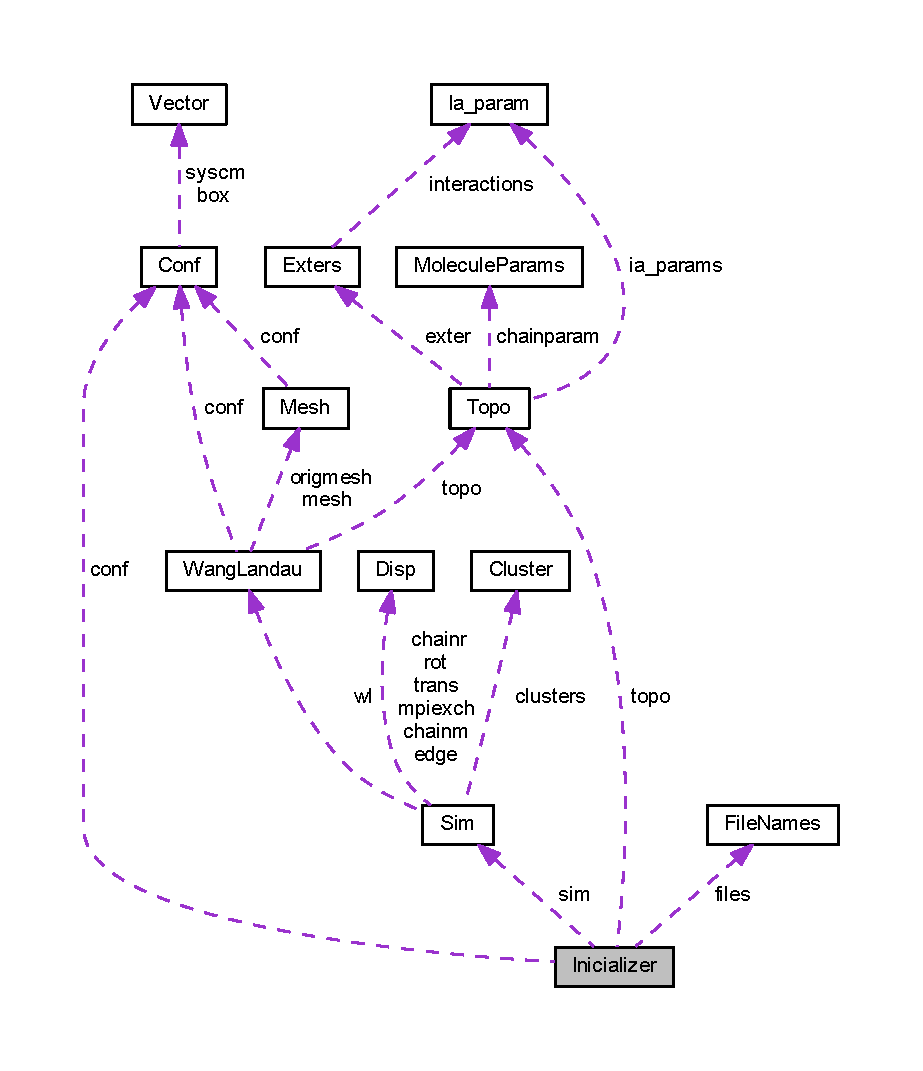
\includegraphics[width=350pt]{class_inicializer__coll__graph}
\end{center}
\end{figure}
\subsection*{Public Member Functions}
\begin{DoxyCompactItemize}
\item 
\hyperlink{class_inicializer_aebd47082aeb8e42a1f44edd8a9844fa1}{Inicializer} (\hyperlink{struct_topo}{Topo} $\ast$\hyperlink{class_inicializer_a9ce346ffecd5ecf76bd4c1c68a3060f7}{topo}, \hyperlink{struct_sim}{Sim} $\ast$\hyperlink{class_inicializer_a8d55514c1121c5d3edbbd4fdfb32db65}{sim}, \hyperlink{class_conf}{Conf} $\ast$\hyperlink{class_inicializer_a6a3bb727f3ad6db5c667f615596cd5e4}{conf}, \hyperlink{struct_file_names}{File\+Names} $\ast$\hyperlink{class_inicializer_aecd4b4dcea44e06dd58000db4144e93e}{files})
\item 
long int \hyperlink{class_inicializer_a8cc93243d56aa21def8f073739f63ad4}{get\+Seed} ()
\item 
void \hyperlink{class_inicializer_a41ac3793bca326b7b0d47c342bebf7b4}{read\+Options} ()
\begin{DoxyCompactList}\small\item\em Reads the run parameters from the external file \char`\"{}options\char`\"{}. See the end of the code for a template. All comments starting with '\#' are stripped out. The options are summarised on standard output and checked for validity of range. \end{DoxyCompactList}\item 
void \hyperlink{class_inicializer_a7e1409d66a770fb50bcd90d96446a917}{init\+Top} ()
\begin{DoxyCompactList}\small\item\em Inicialization of topology. \end{DoxyCompactList}\item 
void \hyperlink{class_inicializer_a03369c6bc8655d42befd4c79f4f02301}{init\+Config} ()
\begin{DoxyCompactList}\small\item\em Config initialization. \end{DoxyCompactList}\item 
void \hyperlink{class_inicializer_a228deba06743d06562179c7f85b958ad}{test\+Chains} ()
\begin{DoxyCompactList}\small\item\em test if simulation contains Chains, sets probability of chain move to 0 if no chains \end{DoxyCompactList}\item 
void \hyperlink{class_inicializer_aa83bb88c8dae21837f025912b2fff68b}{init\+Write\+Files} ()
\begin{DoxyCompactList}\small\item\em Sets names of \char`\"{}write files\char`\"{}. \end{DoxyCompactList}\item 
void \hyperlink{class_inicializer_adbd22bfd9d376b88ab4e1252e752f64b}{init\+Pairlist} ()
\begin{DoxyCompactList}\small\item\em Initializes the pairlist and allocates memory. \end{DoxyCompactList}\item 
void \hyperlink{class_inicializer_afb8f1f23bd87796ae7e66a3917cd1980}{init\+M\+P\+I} ()
\begin{DoxyCompactList}\small\item\em Paralel tempering(\+Replica exchange move) initialization. \end{DoxyCompactList}\end{DoxyCompactItemize}
\subsection*{Private Member Functions}
\begin{DoxyCompactItemize}
\item 
void \hyperlink{class_inicializer_acd2d40a23bdd29b973176c62ab5aef8d}{read\+Topo\+File} (\hyperlink{struct_molecule}{Molecule} $\ast$molecules, long $\ast$sysmoln, char $\ast$sysnames\mbox{[}$\,$\mbox{]}, bool exclusions\mbox{[}$\,$\mbox{]}\mbox{[}\hyperlink{macros_8h_a3f79fdecc884eb98c97d1bdc77455295}{M\+A\+X\+T}\mbox{]})
\item 
void \hyperlink{class_inicializer_a9dd91188a01b07c04f366428bcf2d545}{init\+Chain\+Params} ()
\item 
void \hyperlink{class_inicializer_a216a84344614d74a123f720beab18b62}{init\+Chain\+Lists} ()
\item 
void \hyperlink{class_inicializer_a3613cbdca3c53bb9992978c04a633d94}{init\+Molecules} (\hyperlink{struct_molecule}{Molecule} molecules\mbox{[}\hyperlink{macros_8h_ad002a98462c90c52983b122ab9e2059a}{M\+A\+X\+M\+T}\mbox{]})
\item 
void \hyperlink{class_inicializer_ae0b9e84765b73f78e05aa6c5e99dcc68}{open\+Topo\+File} (F\+I\+L\+E $\ast$infile)
\item 
void \hyperlink{class_inicializer_a1d3e25551f9a48a112d20e9680205d76}{alloc\+Sysmoln} (long $\ast$sysmoln)
\item 
void $\ast$ \hyperlink{class_inicializer_a271a0eef3110b4f1557c7b43d2e0320c}{x\+Malloc} (size\+\_\+t num)
\begin{DoxyCompactList}\small\item\em xmalloc nice malloc, which does the error checking for us \end{DoxyCompactList}\item 
void \hyperlink{class_inicializer_abd279f61f02c065e09384ed1a72831af}{init\+Params} ()
\begin{DoxyCompactList}\small\item\em initialize parameters for interactions \end{DoxyCompactList}\item 
int \hyperlink{class_inicializer_a64fa047683e35560283287c30e269f9a}{top\+Dealoc} (char $\ast$sysnames\mbox{[}\hyperlink{macros_8h_ad1f79d9d99776d7353c6659c307c83c6}{M\+A\+X\+N}\mbox{]}, long $\ast$$\ast$sysmoln, \hyperlink{struct_molecule}{Molecule} $\ast$molecules)
\begin{DoxyCompactList}\small\item\em dealocating memory for init\+Top \end{DoxyCompactList}\item 
int \hyperlink{class_inicializer_a637c5bb05ee307ee3a37a933a28043d0}{fill\+Exclusions} (char $\ast$$\ast$pline, bool exlusions\mbox{[}$\,$\mbox{]}\mbox{[}\hyperlink{macros_8h_a3f79fdecc884eb98c97d1bdc77455295}{M\+A\+X\+T}\mbox{]})
\begin{DoxyCompactList}\small\item\em filling pair for which we exlude attraction interaction. Returns 1 on succes. \end{DoxyCompactList}\item 
int \hyperlink{class_inicializer_a7307f2946c9106e2705aeb3b53fb1c16}{fill\+System} (char $\ast$pline, char $\ast$sysnames\mbox{[}\hyperlink{macros_8h_ad1f79d9d99776d7353c6659c307c83c6}{M\+A\+X\+N}\mbox{]}, long $\ast$$\ast$sysmoln)
\begin{DoxyCompactList}\small\item\em filling the system parameters \end{DoxyCompactList}\item 
int \hyperlink{class_inicializer_ac144054462e36e5ea70ba03785ba0f98}{fill\+Types} (char $\ast$$\ast$pline)
\begin{DoxyCompactList}\small\item\em filing the parameters for types from given strings. Returns 1 on succes. \end{DoxyCompactList}\item 
int \hyperlink{class_inicializer_a5fdd81d2acf5ead8bcc87fab2a2b8809}{convert\+Geotype} (char $\ast$geotype)
\begin{DoxyCompactList}\small\item\em Converts the geometrical type string into a number. \end{DoxyCompactList}\item 
int \hyperlink{class_inicializer_a2e61220db2412742fb203b6c7bcf6b93}{fill\+Exter} (char $\ast$$\ast$pline)
\begin{DoxyCompactList}\small\item\em filling the parameters of external potentail -\/ wall. Returns 1 on succes. \end{DoxyCompactList}\item 
int \hyperlink{class_inicializer_a6dad809b18ec2149abc33d71736b1e7b}{fill\+Mol} (char $\ast$molname, char $\ast$pline, \hyperlink{struct_molecule}{Molecule} $\ast$molecules)
\begin{DoxyCompactList}\small\item\em filling the parameters for molecules \end{DoxyCompactList}\item 
void \hyperlink{class_inicializer_af2a4f4721e9105cda901ae4d5530fd43}{gen\+Param\+Pairs} (bool($\ast$exclusions)\mbox{[}\hyperlink{macros_8h_a3f79fdecc884eb98c97d1bdc77455295}{M\+A\+X\+T}\mbox{]}\mbox{[}\hyperlink{macros_8h_a3f79fdecc884eb98c97d1bdc77455295}{M\+A\+X\+T}\mbox{]})
\begin{DoxyCompactList}\small\item\em generate interations pairs \end{DoxyCompactList}\item 
void \hyperlink{class_inicializer_ac5d3d17ceb46d4096e173fa373bd12f6}{use\+P\+B\+C} (\hyperlink{class_vector}{Vector} $\ast$pos, \hyperlink{class_vector}{Vector} pbc)
\begin{DoxyCompactList}\small\item\em use of periodic boundary conditions \end{DoxyCompactList}\item 
void \hyperlink{class_inicializer_a59b1de21fff55d47d71f1e3f56a6b23f}{readii2} (char $\ast$num, int value\mbox{[}2\mbox{]})
\begin{DoxyCompactList}\small\item\em convert string num into two integers \end{DoxyCompactList}\item 
double \hyperlink{class_inicializer_a93fa1c3e89f1a519611e9861d9f30989}{readd2} (char $\ast$num)
\begin{DoxyCompactList}\small\item\em convert string num into double \end{DoxyCompactList}\item 
long \hyperlink{class_inicializer_added4b028cc3d6118d1b8c92c3eedd82}{readl2} (char $\ast$num)
\begin{DoxyCompactList}\small\item\em convert string num into long \end{DoxyCompactList}\item 
int \hyperlink{class_inicializer_ab20cbac5cc1211b24da005557a67ea10}{readi2} (char $\ast$num)
\begin{DoxyCompactList}\small\item\em convert string num into integer \end{DoxyCompactList}\end{DoxyCompactItemize}
\subsection*{Private Attributes}
\begin{DoxyCompactItemize}
\item 
long \hyperlink{class_inicializer_a98c446c361d34327e838a17737126212}{seed}
\item 
\hyperlink{struct_topo}{Topo} $\ast$ \hyperlink{class_inicializer_a9ce346ffecd5ecf76bd4c1c68a3060f7}{topo}
\item 
\hyperlink{struct_sim}{Sim} $\ast$ \hyperlink{class_inicializer_a8d55514c1121c5d3edbbd4fdfb32db65}{sim}
\item 
\hyperlink{class_conf}{Conf} $\ast$ \hyperlink{class_inicializer_a6a3bb727f3ad6db5c667f615596cd5e4}{conf}
\item 
\hyperlink{struct_file_names}{File\+Names} $\ast$ \hyperlink{class_inicializer_aecd4b4dcea44e06dd58000db4144e93e}{files}
\end{DoxyCompactItemize}


\subsection{Constructor \& Destructor Documentation}
\hypertarget{class_inicializer_aebd47082aeb8e42a1f44edd8a9844fa1}{\index{Inicializer@{Inicializer}!Inicializer@{Inicializer}}
\index{Inicializer@{Inicializer}!Inicializer@{Inicializer}}
\subsubsection[{Inicializer}]{\setlength{\rightskip}{0pt plus 5cm}Inicializer\+::\+Inicializer (
\begin{DoxyParamCaption}
\item[{{\bf Topo} $\ast$}]{topo, }
\item[{{\bf Sim} $\ast$}]{sim, }
\item[{{\bf Conf} $\ast$}]{conf, }
\item[{{\bf File\+Names} $\ast$}]{files}
\end{DoxyParamCaption}
)\hspace{0.3cm}{\ttfamily [inline]}}}\label{class_inicializer_aebd47082aeb8e42a1f44edd8a9844fa1}


\subsection{Member Function Documentation}
\hypertarget{class_inicializer_a1d3e25551f9a48a112d20e9680205d76}{\index{Inicializer@{Inicializer}!alloc\+Sysmoln@{alloc\+Sysmoln}}
\index{alloc\+Sysmoln@{alloc\+Sysmoln}!Inicializer@{Inicializer}}
\subsubsection[{alloc\+Sysmoln}]{\setlength{\rightskip}{0pt plus 5cm}void Inicializer\+::alloc\+Sysmoln (
\begin{DoxyParamCaption}
\item[{long $\ast$}]{sysmoln}
\end{DoxyParamCaption}
)\hspace{0.3cm}{\ttfamily [private]}}}\label{class_inicializer_a1d3e25551f9a48a112d20e9680205d76}
\hypertarget{class_inicializer_a5fdd81d2acf5ead8bcc87fab2a2b8809}{\index{Inicializer@{Inicializer}!convert\+Geotype@{convert\+Geotype}}
\index{convert\+Geotype@{convert\+Geotype}!Inicializer@{Inicializer}}
\subsubsection[{convert\+Geotype}]{\setlength{\rightskip}{0pt plus 5cm}int Inicializer\+::convert\+Geotype (
\begin{DoxyParamCaption}
\item[{char $\ast$}]{geotype}
\end{DoxyParamCaption}
)\hspace{0.3cm}{\ttfamily [private]}}}\label{class_inicializer_a5fdd81d2acf5ead8bcc87fab2a2b8809}


Converts the geometrical type string into a number. 


\begin{DoxyParams}{Parameters}
{\em geotype} & \\
\hline
\end{DoxyParams}
\begin{DoxyReturn}{Returns}

\end{DoxyReturn}


Here is the caller graph for this function\+:\nopagebreak
\begin{figure}[H]
\begin{center}
\leavevmode
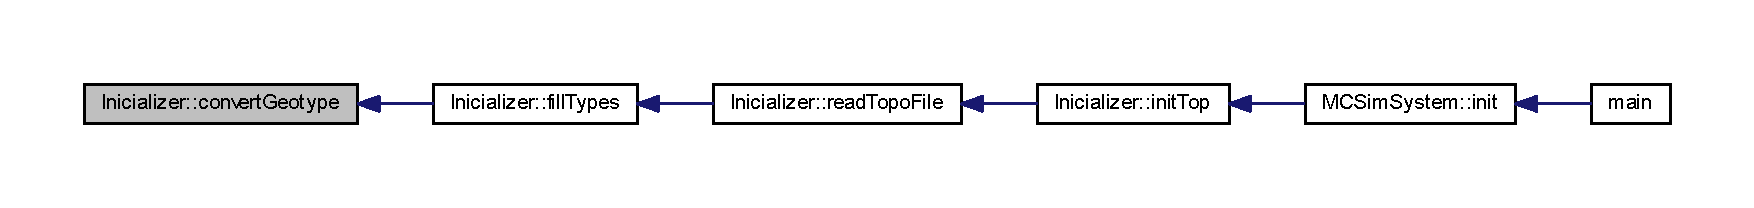
\includegraphics[width=350pt]{class_inicializer_a5fdd81d2acf5ead8bcc87fab2a2b8809_icgraph}
\end{center}
\end{figure}


\hypertarget{class_inicializer_a637c5bb05ee307ee3a37a933a28043d0}{\index{Inicializer@{Inicializer}!fill\+Exclusions@{fill\+Exclusions}}
\index{fill\+Exclusions@{fill\+Exclusions}!Inicializer@{Inicializer}}
\subsubsection[{fill\+Exclusions}]{\setlength{\rightskip}{0pt plus 5cm}int Inicializer\+::fill\+Exclusions (
\begin{DoxyParamCaption}
\item[{char $\ast$$\ast$}]{pline, }
\item[{bool}]{exlusions\mbox{[}$\,$\mbox{]}\mbox{[}\+M\+A\+X\+T\mbox{]}}
\end{DoxyParamCaption}
)\hspace{0.3cm}{\ttfamily [private]}}}\label{class_inicializer_a637c5bb05ee307ee3a37a933a28043d0}


filling pair for which we exlude attraction interaction. Returns 1 on succes. 


\begin{DoxyParams}{Parameters}
{\em pline} & \\
\hline
{\em ($\ast$exlusions)\mbox{[}$\,$\mbox{]}\mbox{[}$\,$\mbox{]}} & \\
\hline
\end{DoxyParams}
\begin{DoxyReturn}{Returns}

\end{DoxyReturn}


Here is the call graph for this function\+:\nopagebreak
\begin{figure}[H]
\begin{center}
\leavevmode
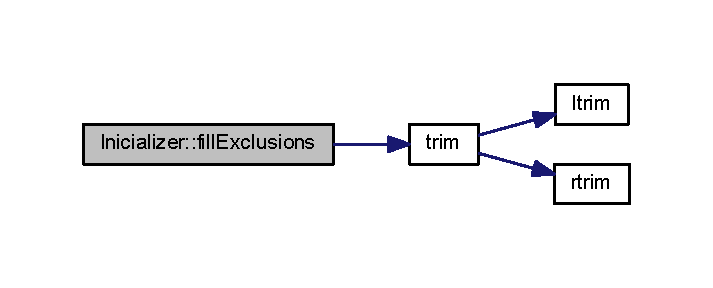
\includegraphics[width=342pt]{class_inicializer_a637c5bb05ee307ee3a37a933a28043d0_cgraph}
\end{center}
\end{figure}




Here is the caller graph for this function\+:\nopagebreak
\begin{figure}[H]
\begin{center}
\leavevmode
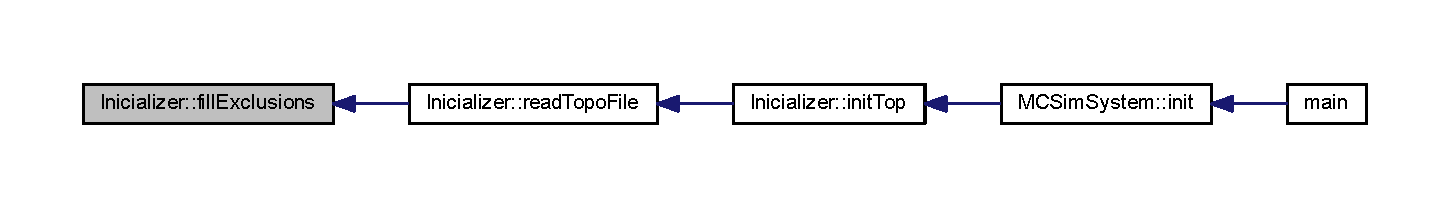
\includegraphics[width=350pt]{class_inicializer_a637c5bb05ee307ee3a37a933a28043d0_icgraph}
\end{center}
\end{figure}


\hypertarget{class_inicializer_a2e61220db2412742fb203b6c7bcf6b93}{\index{Inicializer@{Inicializer}!fill\+Exter@{fill\+Exter}}
\index{fill\+Exter@{fill\+Exter}!Inicializer@{Inicializer}}
\subsubsection[{fill\+Exter}]{\setlength{\rightskip}{0pt plus 5cm}int Inicializer\+::fill\+Exter (
\begin{DoxyParamCaption}
\item[{char $\ast$$\ast$}]{pline}
\end{DoxyParamCaption}
)\hspace{0.3cm}{\ttfamily [private]}}}\label{class_inicializer_a2e61220db2412742fb203b6c7bcf6b93}


filling the parameters of external potentail -\/ wall. Returns 1 on succes. 


\begin{DoxyParams}{Parameters}
{\em pline} & \\
\hline
\end{DoxyParams}
\begin{DoxyReturn}{Returns}

\end{DoxyReturn}


Here is the call graph for this function\+:\nopagebreak
\begin{figure}[H]
\begin{center}
\leavevmode
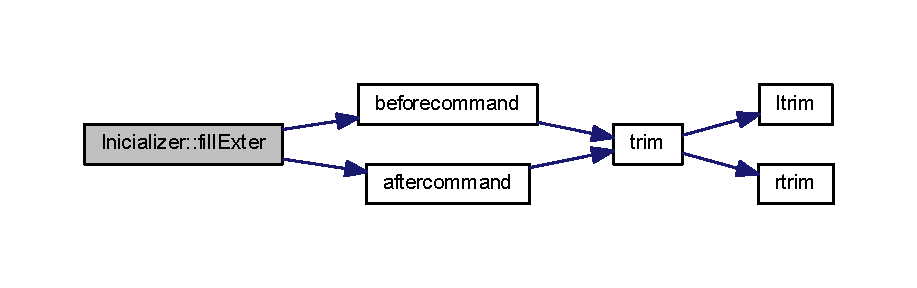
\includegraphics[width=350pt]{class_inicializer_a2e61220db2412742fb203b6c7bcf6b93_cgraph}
\end{center}
\end{figure}




Here is the caller graph for this function\+:\nopagebreak
\begin{figure}[H]
\begin{center}
\leavevmode
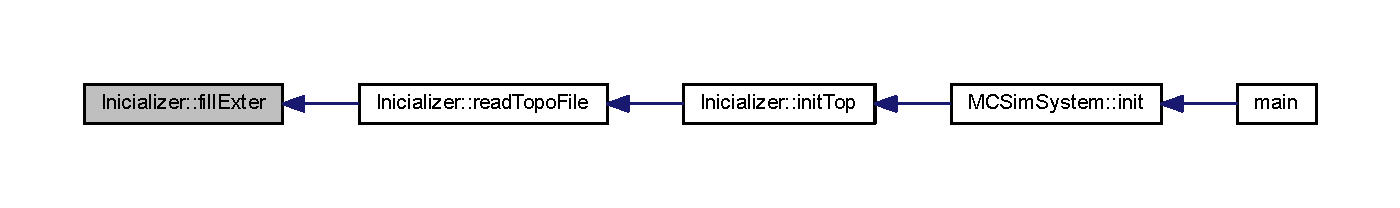
\includegraphics[width=350pt]{class_inicializer_a2e61220db2412742fb203b6c7bcf6b93_icgraph}
\end{center}
\end{figure}


\hypertarget{class_inicializer_a6dad809b18ec2149abc33d71736b1e7b}{\index{Inicializer@{Inicializer}!fill\+Mol@{fill\+Mol}}
\index{fill\+Mol@{fill\+Mol}!Inicializer@{Inicializer}}
\subsubsection[{fill\+Mol}]{\setlength{\rightskip}{0pt plus 5cm}int Inicializer\+::fill\+Mol (
\begin{DoxyParamCaption}
\item[{char $\ast$}]{molname, }
\item[{char $\ast$}]{pline, }
\item[{{\bf Molecule} $\ast$}]{molecules}
\end{DoxyParamCaption}
)\hspace{0.3cm}{\ttfamily [private]}}}\label{class_inicializer_a6dad809b18ec2149abc33d71736b1e7b}


filling the parameters for molecules 


\begin{DoxyParams}{Parameters}
{\em molname} & \\
\hline
{\em pline} & \\
\hline
{\em molecules} & \\
\hline
\end{DoxyParams}
\begin{DoxyReturn}{Returns}

\end{DoxyReturn}
I\+N\+I\+T of mu\+V\+T ensemble 

Here is the call graph for this function\+:\nopagebreak
\begin{figure}[H]
\begin{center}
\leavevmode
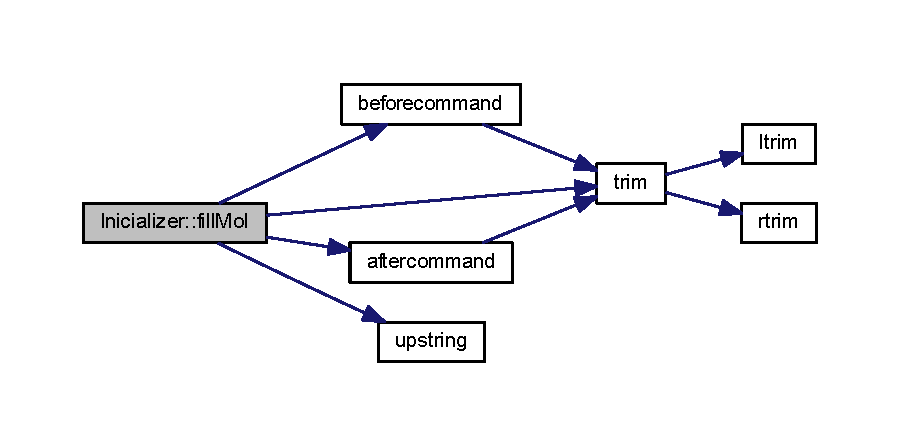
\includegraphics[width=350pt]{class_inicializer_a6dad809b18ec2149abc33d71736b1e7b_cgraph}
\end{center}
\end{figure}




Here is the caller graph for this function\+:\nopagebreak
\begin{figure}[H]
\begin{center}
\leavevmode
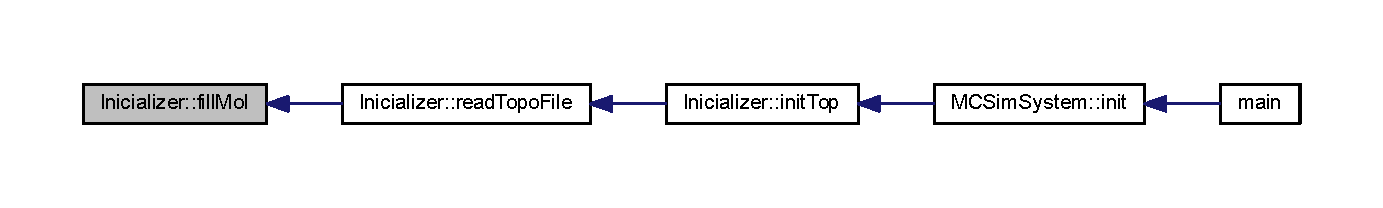
\includegraphics[width=350pt]{class_inicializer_a6dad809b18ec2149abc33d71736b1e7b_icgraph}
\end{center}
\end{figure}


\hypertarget{class_inicializer_a7307f2946c9106e2705aeb3b53fb1c16}{\index{Inicializer@{Inicializer}!fill\+System@{fill\+System}}
\index{fill\+System@{fill\+System}!Inicializer@{Inicializer}}
\subsubsection[{fill\+System}]{\setlength{\rightskip}{0pt plus 5cm}int Inicializer\+::fill\+System (
\begin{DoxyParamCaption}
\item[{char $\ast$}]{pline, }
\item[{char $\ast$}]{sysnames\mbox{[}\+M\+A\+X\+N\mbox{]}, }
\item[{long $\ast$$\ast$}]{sysmoln}
\end{DoxyParamCaption}
)\hspace{0.3cm}{\ttfamily [private]}}}\label{class_inicializer_a7307f2946c9106e2705aeb3b53fb1c16}


filling the system parameters 


\begin{DoxyParams}{Parameters}
{\em pline} & \\
\hline
{\em sysnames} & \\
\hline
{\em sysmoln} & \\
\hline
\end{DoxyParams}
\begin{DoxyReturn}{Returns}

\end{DoxyReturn}


Here is the call graph for this function\+:\nopagebreak
\begin{figure}[H]
\begin{center}
\leavevmode
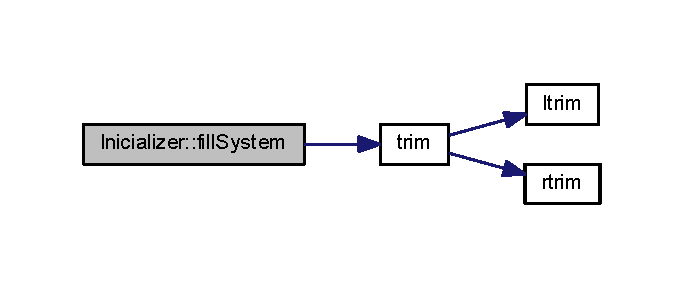
\includegraphics[width=328pt]{class_inicializer_a7307f2946c9106e2705aeb3b53fb1c16_cgraph}
\end{center}
\end{figure}




Here is the caller graph for this function\+:\nopagebreak
\begin{figure}[H]
\begin{center}
\leavevmode
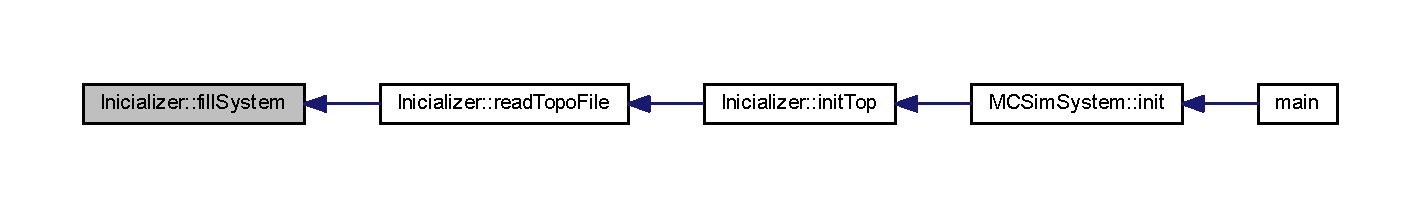
\includegraphics[width=350pt]{class_inicializer_a7307f2946c9106e2705aeb3b53fb1c16_icgraph}
\end{center}
\end{figure}


\hypertarget{class_inicializer_ac144054462e36e5ea70ba03785ba0f98}{\index{Inicializer@{Inicializer}!fill\+Types@{fill\+Types}}
\index{fill\+Types@{fill\+Types}!Inicializer@{Inicializer}}
\subsubsection[{fill\+Types}]{\setlength{\rightskip}{0pt plus 5cm}int Inicializer\+::fill\+Types (
\begin{DoxyParamCaption}
\item[{char $\ast$$\ast$}]{pline}
\end{DoxyParamCaption}
)\hspace{0.3cm}{\ttfamily [private]}}}\label{class_inicializer_ac144054462e36e5ea70ba03785ba0f98}


filing the parameters for types from given strings. Returns 1 on succes. 


\begin{DoxyParams}{Parameters}
{\em pline} & \\
\hline
\end{DoxyParams}
\begin{DoxyReturn}{Returns}

\end{DoxyReturn}


Here is the call graph for this function\+:\nopagebreak
\begin{figure}[H]
\begin{center}
\leavevmode
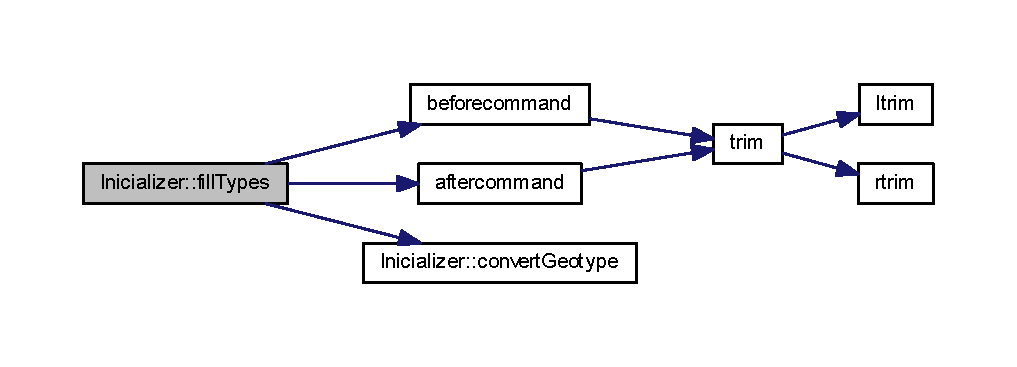
\includegraphics[width=350pt]{class_inicializer_ac144054462e36e5ea70ba03785ba0f98_cgraph}
\end{center}
\end{figure}




Here is the caller graph for this function\+:\nopagebreak
\begin{figure}[H]
\begin{center}
\leavevmode
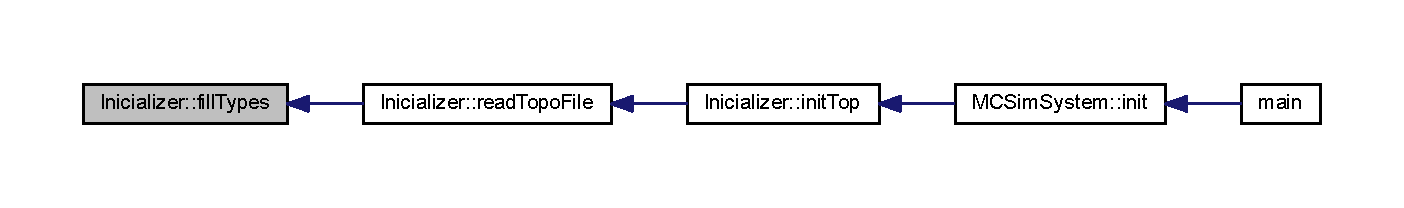
\includegraphics[width=350pt]{class_inicializer_ac144054462e36e5ea70ba03785ba0f98_icgraph}
\end{center}
\end{figure}


\hypertarget{class_inicializer_af2a4f4721e9105cda901ae4d5530fd43}{\index{Inicializer@{Inicializer}!gen\+Param\+Pairs@{gen\+Param\+Pairs}}
\index{gen\+Param\+Pairs@{gen\+Param\+Pairs}!Inicializer@{Inicializer}}
\subsubsection[{gen\+Param\+Pairs}]{\setlength{\rightskip}{0pt plus 5cm}void Inicializer\+::gen\+Param\+Pairs (
\begin{DoxyParamCaption}
\item[{bool($\ast$)}]{exclusions\mbox{[}\+M\+A\+X\+T\mbox{]}\mbox{[}\+M\+A\+X\+T\mbox{]}}
\end{DoxyParamCaption}
)\hspace{0.3cm}{\ttfamily [private]}}}\label{class_inicializer_af2a4f4721e9105cda901ae4d5530fd43}


generate interations pairs 


\begin{DoxyParams}{Parameters}
{\em ($\ast$exlusions)\mbox{[}$\,$\mbox{]}\mbox{[}$\,$\mbox{]}} & \\
\hline
\end{DoxyParams}


Here is the caller graph for this function\+:\nopagebreak
\begin{figure}[H]
\begin{center}
\leavevmode
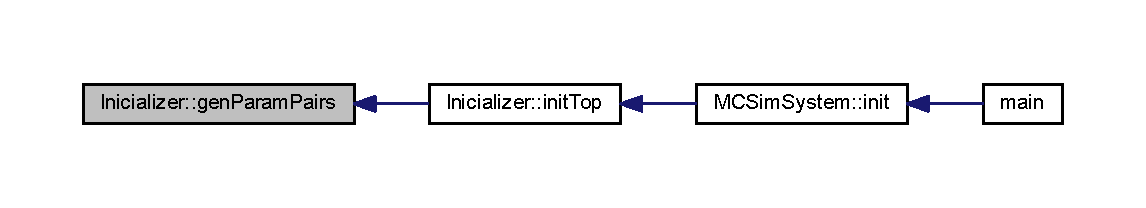
\includegraphics[width=350pt]{class_inicializer_af2a4f4721e9105cda901ae4d5530fd43_icgraph}
\end{center}
\end{figure}


\hypertarget{class_inicializer_a8cc93243d56aa21def8f073739f63ad4}{\index{Inicializer@{Inicializer}!get\+Seed@{get\+Seed}}
\index{get\+Seed@{get\+Seed}!Inicializer@{Inicializer}}
\subsubsection[{get\+Seed}]{\setlength{\rightskip}{0pt plus 5cm}long int Inicializer\+::get\+Seed (
\begin{DoxyParamCaption}
{}
\end{DoxyParamCaption}
)\hspace{0.3cm}{\ttfamily [inline]}}}\label{class_inicializer_a8cc93243d56aa21def8f073739f63ad4}


Here is the caller graph for this function\+:\nopagebreak
\begin{figure}[H]
\begin{center}
\leavevmode
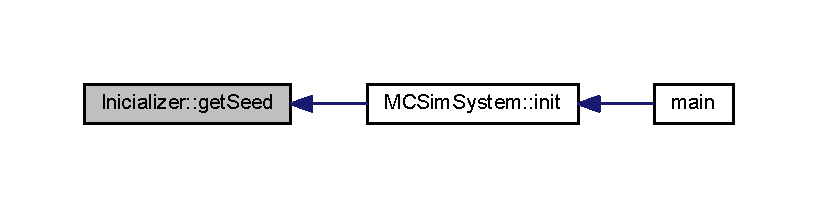
\includegraphics[width=350pt]{class_inicializer_a8cc93243d56aa21def8f073739f63ad4_icgraph}
\end{center}
\end{figure}


\hypertarget{class_inicializer_a216a84344614d74a123f720beab18b62}{\index{Inicializer@{Inicializer}!init\+Chain\+Lists@{init\+Chain\+Lists}}
\index{init\+Chain\+Lists@{init\+Chain\+Lists}!Inicializer@{Inicializer}}
\subsubsection[{init\+Chain\+Lists}]{\setlength{\rightskip}{0pt plus 5cm}void Inicializer\+::init\+Chain\+Lists (
\begin{DoxyParamCaption}
{}
\end{DoxyParamCaption}
)\hspace{0.3cm}{\ttfamily [private]}}}\label{class_inicializer_a216a84344614d74a123f720beab18b62}


Here is the caller graph for this function\+:\nopagebreak
\begin{figure}[H]
\begin{center}
\leavevmode
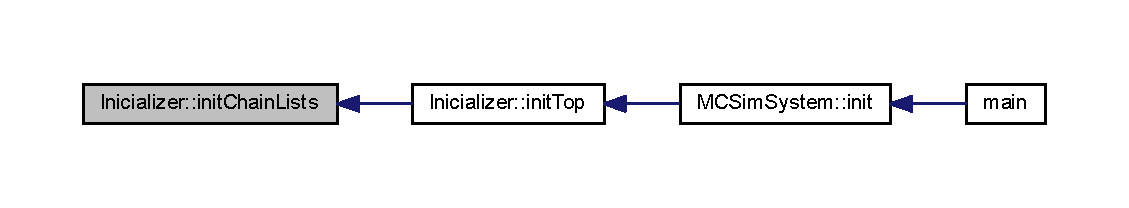
\includegraphics[width=350pt]{class_inicializer_a216a84344614d74a123f720beab18b62_icgraph}
\end{center}
\end{figure}


\hypertarget{class_inicializer_a9dd91188a01b07c04f366428bcf2d545}{\index{Inicializer@{Inicializer}!init\+Chain\+Params@{init\+Chain\+Params}}
\index{init\+Chain\+Params@{init\+Chain\+Params}!Inicializer@{Inicializer}}
\subsubsection[{init\+Chain\+Params}]{\setlength{\rightskip}{0pt plus 5cm}void Inicializer\+::init\+Chain\+Params (
\begin{DoxyParamCaption}
{}
\end{DoxyParamCaption}
)\hspace{0.3cm}{\ttfamily [private]}}}\label{class_inicializer_a9dd91188a01b07c04f366428bcf2d545}


Here is the caller graph for this function\+:\nopagebreak
\begin{figure}[H]
\begin{center}
\leavevmode
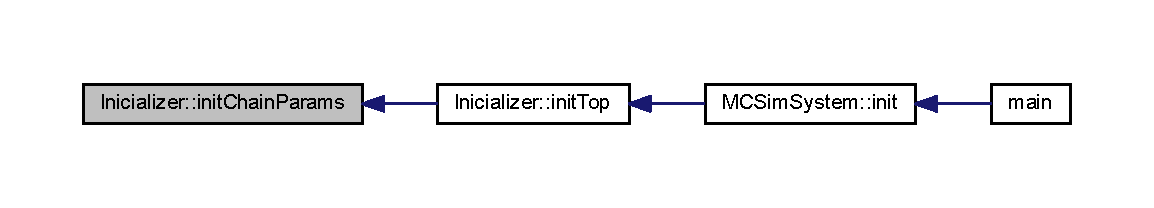
\includegraphics[width=350pt]{class_inicializer_a9dd91188a01b07c04f366428bcf2d545_icgraph}
\end{center}
\end{figure}


\hypertarget{class_inicializer_a03369c6bc8655d42befd4c79f4f02301}{\index{Inicializer@{Inicializer}!init\+Config@{init\+Config}}
\index{init\+Config@{init\+Config}!Inicializer@{Inicializer}}
\subsubsection[{init\+Config}]{\setlength{\rightskip}{0pt plus 5cm}void Inicializer\+::init\+Config (
\begin{DoxyParamCaption}
{}
\end{DoxyParamCaption}
)}}\label{class_inicializer_a03369c6bc8655d42befd4c79f4f02301}


Config initialization. 

Reads in the initial configuration from the file \char`\"{}config.\+init\char`\"{}. Each line contains the three components of the position vector and three components of the direction vector and three components of patch direction for a spherocylinder. The direction vector is normalised after being read in. The configuration is checked for particle overlaps. 

Here is the call graph for this function\+:\nopagebreak
\begin{figure}[H]
\begin{center}
\leavevmode
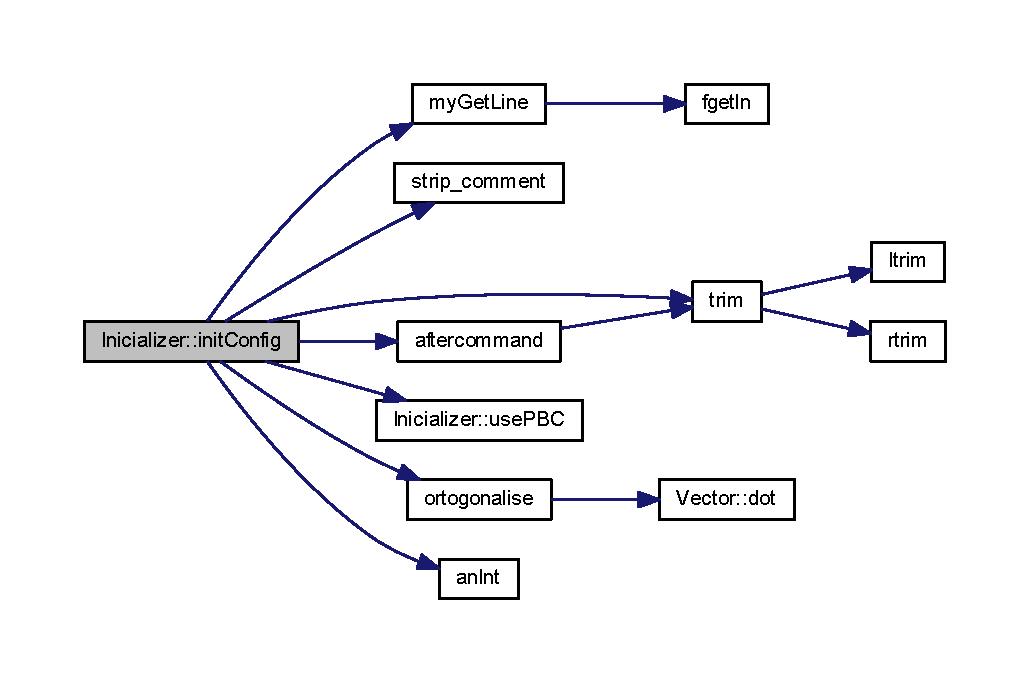
\includegraphics[width=350pt]{class_inicializer_a03369c6bc8655d42befd4c79f4f02301_cgraph}
\end{center}
\end{figure}




Here is the caller graph for this function\+:\nopagebreak
\begin{figure}[H]
\begin{center}
\leavevmode
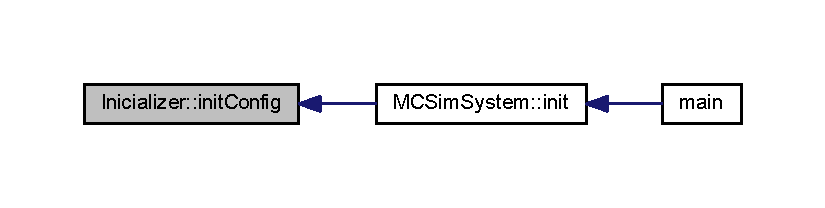
\includegraphics[width=350pt]{class_inicializer_a03369c6bc8655d42befd4c79f4f02301_icgraph}
\end{center}
\end{figure}


\hypertarget{class_inicializer_a3613cbdca3c53bb9992978c04a633d94}{\index{Inicializer@{Inicializer}!init\+Molecules@{init\+Molecules}}
\index{init\+Molecules@{init\+Molecules}!Inicializer@{Inicializer}}
\subsubsection[{init\+Molecules}]{\setlength{\rightskip}{0pt plus 5cm}void Inicializer\+::init\+Molecules (
\begin{DoxyParamCaption}
\item[{{\bf Molecule}}]{molecules\mbox{[}\+M\+A\+X\+M\+T\mbox{]}}
\end{DoxyParamCaption}
)\hspace{0.3cm}{\ttfamily [private]}}}\label{class_inicializer_a3613cbdca3c53bb9992978c04a633d94}


Here is the caller graph for this function\+:\nopagebreak
\begin{figure}[H]
\begin{center}
\leavevmode
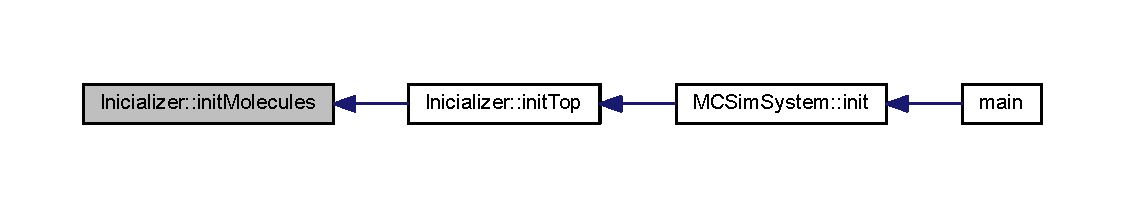
\includegraphics[width=350pt]{class_inicializer_a3613cbdca3c53bb9992978c04a633d94_icgraph}
\end{center}
\end{figure}


\hypertarget{class_inicializer_afb8f1f23bd87796ae7e66a3917cd1980}{\index{Inicializer@{Inicializer}!init\+M\+P\+I@{init\+M\+P\+I}}
\index{init\+M\+P\+I@{init\+M\+P\+I}!Inicializer@{Inicializer}}
\subsubsection[{init\+M\+P\+I}]{\setlength{\rightskip}{0pt plus 5cm}void Inicializer\+::init\+M\+P\+I (
\begin{DoxyParamCaption}
{}
\end{DoxyParamCaption}
)}}\label{class_inicializer_afb8f1f23bd87796ae7e66a3917cd1980}


Paralel tempering(\+Replica exchange move) initialization. 



Here is the caller graph for this function\+:\nopagebreak
\begin{figure}[H]
\begin{center}
\leavevmode
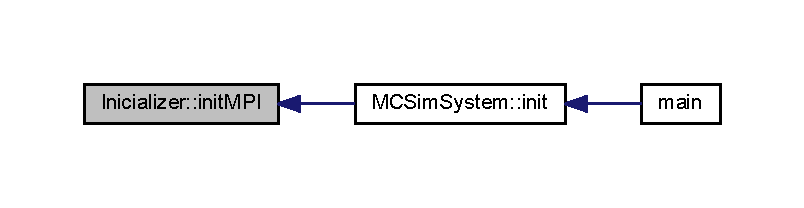
\includegraphics[width=350pt]{class_inicializer_afb8f1f23bd87796ae7e66a3917cd1980_icgraph}
\end{center}
\end{figure}


\hypertarget{class_inicializer_adbd22bfd9d376b88ab4e1252e752f64b}{\index{Inicializer@{Inicializer}!init\+Pairlist@{init\+Pairlist}}
\index{init\+Pairlist@{init\+Pairlist}!Inicializer@{Inicializer}}
\subsubsection[{init\+Pairlist}]{\setlength{\rightskip}{0pt plus 5cm}void Inicializer\+::init\+Pairlist (
\begin{DoxyParamCaption}
{}
\end{DoxyParamCaption}
)}}\label{class_inicializer_adbd22bfd9d376b88ab4e1252e752f64b}


Initializes the pairlist and allocates memory. 



Here is the caller graph for this function\+:\nopagebreak
\begin{figure}[H]
\begin{center}
\leavevmode
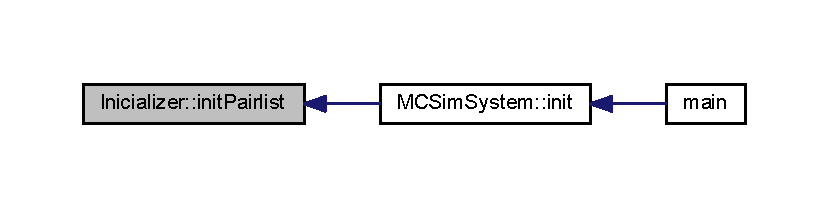
\includegraphics[width=350pt]{class_inicializer_adbd22bfd9d376b88ab4e1252e752f64b_icgraph}
\end{center}
\end{figure}


\hypertarget{class_inicializer_abd279f61f02c065e09384ed1a72831af}{\index{Inicializer@{Inicializer}!init\+Params@{init\+Params}}
\index{init\+Params@{init\+Params}!Inicializer@{Inicializer}}
\subsubsection[{init\+Params}]{\setlength{\rightskip}{0pt plus 5cm}void Inicializer\+::init\+Params (
\begin{DoxyParamCaption}
{}
\end{DoxyParamCaption}
)\hspace{0.3cm}{\ttfamily [private]}}}\label{class_inicializer_abd279f61f02c065e09384ed1a72831af}


initialize parameters for interactions 



Here is the caller graph for this function\+:\nopagebreak
\begin{figure}[H]
\begin{center}
\leavevmode
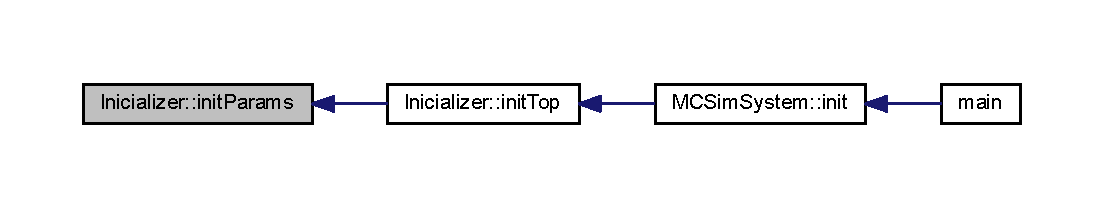
\includegraphics[width=350pt]{class_inicializer_abd279f61f02c065e09384ed1a72831af_icgraph}
\end{center}
\end{figure}


\hypertarget{class_inicializer_a7e1409d66a770fb50bcd90d96446a917}{\index{Inicializer@{Inicializer}!init\+Top@{init\+Top}}
\index{init\+Top@{init\+Top}!Inicializer@{Inicializer}}
\subsubsection[{init\+Top}]{\setlength{\rightskip}{0pt plus 5cm}void Inicializer\+::init\+Top (
\begin{DoxyParamCaption}
{}
\end{DoxyParamCaption}
)}}\label{class_inicializer_a7e1409d66a770fb50bcd90d96446a917}


Inicialization of topology. 

Create lists for chain operations\+: Connectivity list where it is written for each sc with which sc it is connected. The order is important because spherocylinders have direction First is interacting tail then head. Chain list where particles are assigned to chains to which they belong count mu\+V\+T particles 

Here is the call graph for this function\+:\nopagebreak
\begin{figure}[H]
\begin{center}
\leavevmode
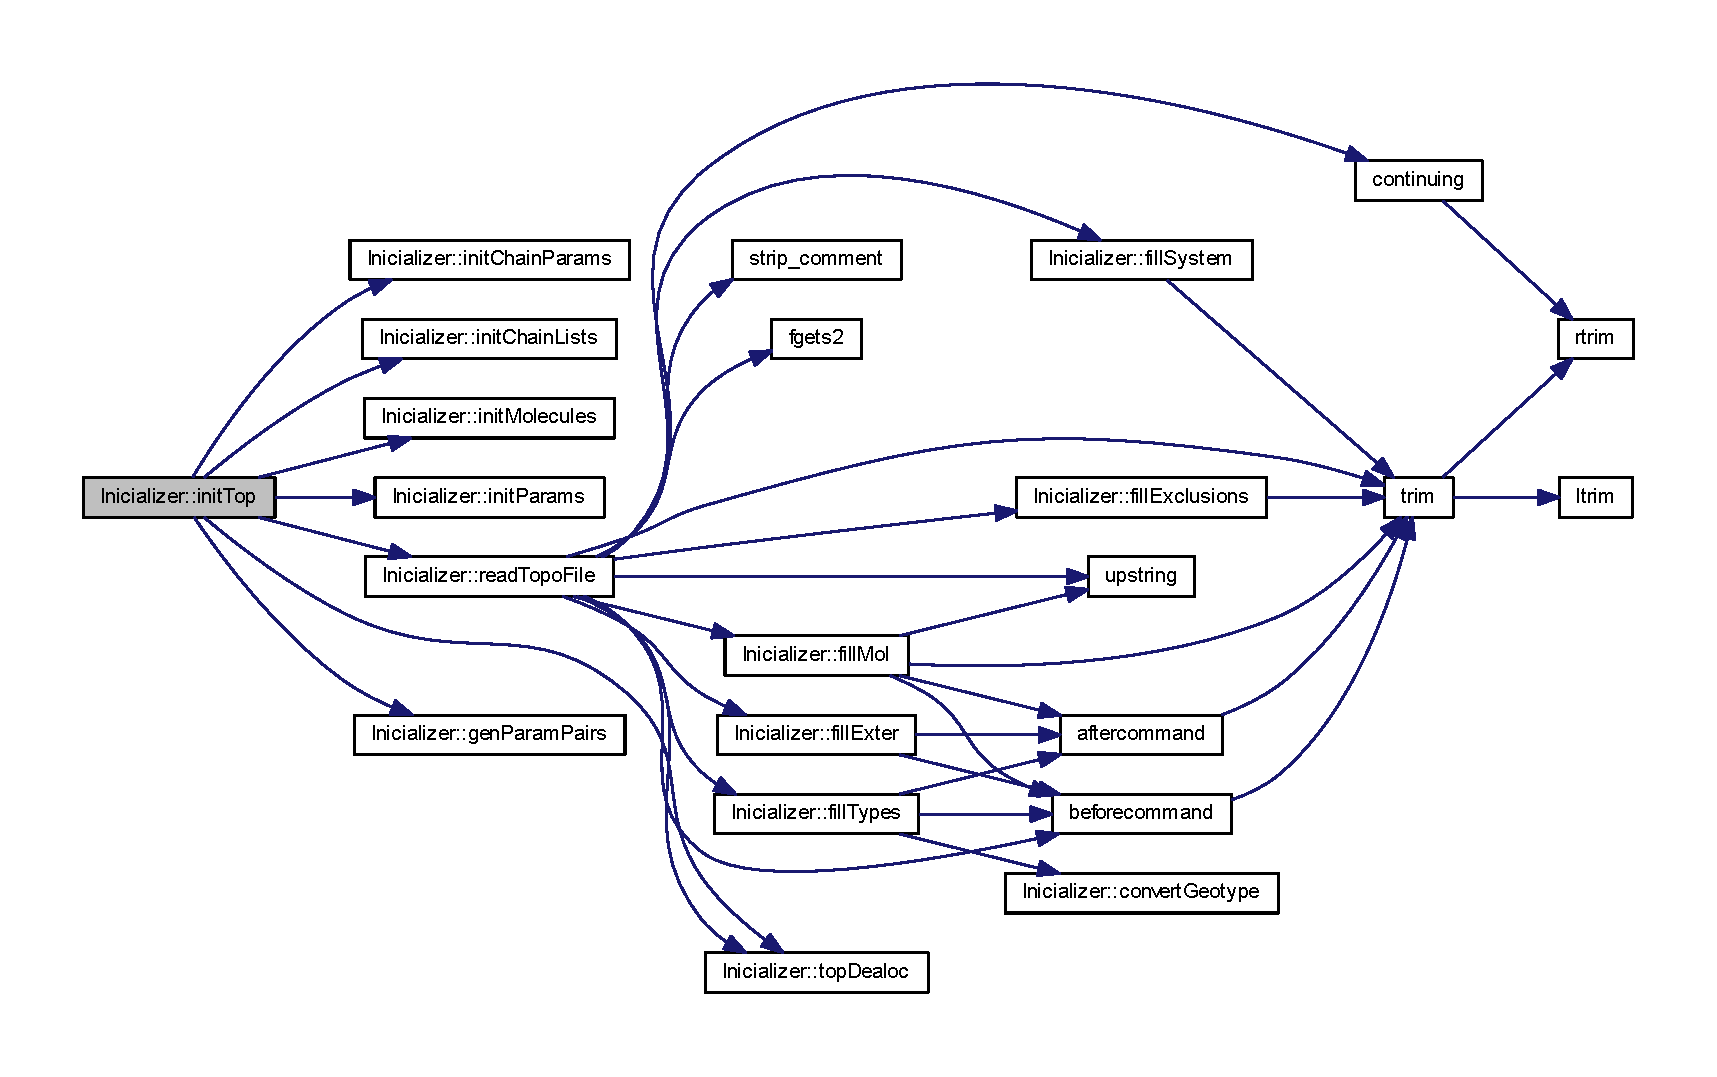
\includegraphics[width=350pt]{class_inicializer_a7e1409d66a770fb50bcd90d96446a917_cgraph}
\end{center}
\end{figure}




Here is the caller graph for this function\+:\nopagebreak
\begin{figure}[H]
\begin{center}
\leavevmode
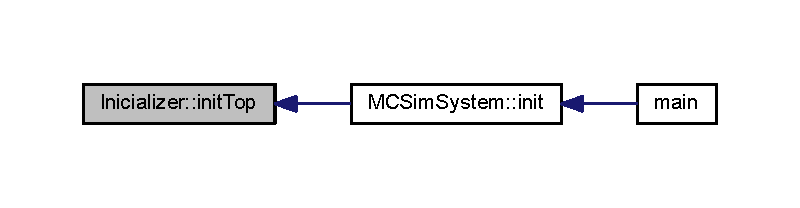
\includegraphics[width=350pt]{class_inicializer_a7e1409d66a770fb50bcd90d96446a917_icgraph}
\end{center}
\end{figure}


\hypertarget{class_inicializer_aa83bb88c8dae21837f025912b2fff68b}{\index{Inicializer@{Inicializer}!init\+Write\+Files@{init\+Write\+Files}}
\index{init\+Write\+Files@{init\+Write\+Files}!Inicializer@{Inicializer}}
\subsubsection[{init\+Write\+Files}]{\setlength{\rightskip}{0pt plus 5cm}void Inicializer\+::init\+Write\+Files (
\begin{DoxyParamCaption}
{}
\end{DoxyParamCaption}
)}}\label{class_inicializer_aa83bb88c8dae21837f025912b2fff68b}


Sets names of \char`\"{}write files\char`\"{}. 



Here is the caller graph for this function\+:\nopagebreak
\begin{figure}[H]
\begin{center}
\leavevmode
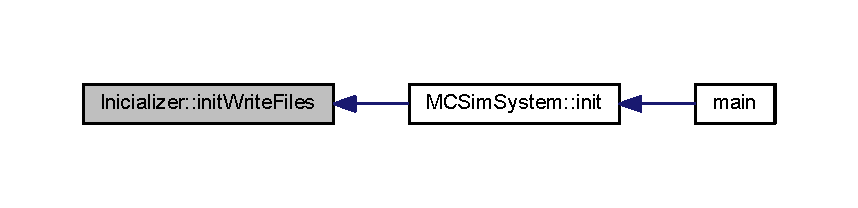
\includegraphics[width=350pt]{class_inicializer_aa83bb88c8dae21837f025912b2fff68b_icgraph}
\end{center}
\end{figure}


\hypertarget{class_inicializer_ae0b9e84765b73f78e05aa6c5e99dcc68}{\index{Inicializer@{Inicializer}!open\+Topo\+File@{open\+Topo\+File}}
\index{open\+Topo\+File@{open\+Topo\+File}!Inicializer@{Inicializer}}
\subsubsection[{open\+Topo\+File}]{\setlength{\rightskip}{0pt plus 5cm}void Inicializer\+::open\+Topo\+File (
\begin{DoxyParamCaption}
\item[{F\+I\+L\+E $\ast$}]{infile}
\end{DoxyParamCaption}
)\hspace{0.3cm}{\ttfamily [private]}}}\label{class_inicializer_ae0b9e84765b73f78e05aa6c5e99dcc68}
\hypertarget{class_inicializer_a93fa1c3e89f1a519611e9861d9f30989}{\index{Inicializer@{Inicializer}!readd2@{readd2}}
\index{readd2@{readd2}!Inicializer@{Inicializer}}
\subsubsection[{readd2}]{\setlength{\rightskip}{0pt plus 5cm}double Inicializer\+::readd2 (
\begin{DoxyParamCaption}
\item[{char $\ast$}]{num}
\end{DoxyParamCaption}
)\hspace{0.3cm}{\ttfamily [private]}}}\label{class_inicializer_a93fa1c3e89f1a519611e9861d9f30989}


convert string num into double 


\begin{DoxyParams}{Parameters}
{\em num} & \\
\hline
\end{DoxyParams}
\begin{DoxyReturn}{Returns}

\end{DoxyReturn}


Here is the caller graph for this function\+:\nopagebreak
\begin{figure}[H]
\begin{center}
\leavevmode
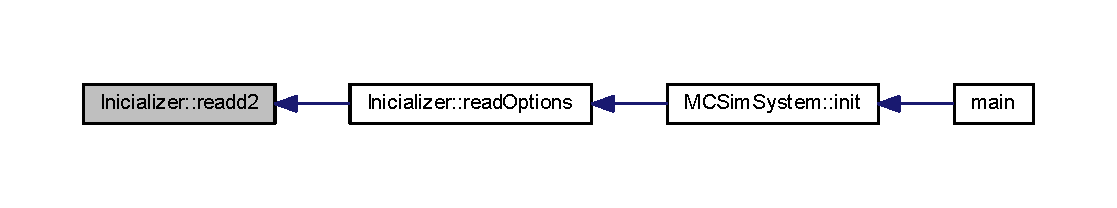
\includegraphics[width=350pt]{class_inicializer_a93fa1c3e89f1a519611e9861d9f30989_icgraph}
\end{center}
\end{figure}


\hypertarget{class_inicializer_ab20cbac5cc1211b24da005557a67ea10}{\index{Inicializer@{Inicializer}!readi2@{readi2}}
\index{readi2@{readi2}!Inicializer@{Inicializer}}
\subsubsection[{readi2}]{\setlength{\rightskip}{0pt plus 5cm}int Inicializer\+::readi2 (
\begin{DoxyParamCaption}
\item[{char $\ast$}]{num}
\end{DoxyParamCaption}
)\hspace{0.3cm}{\ttfamily [private]}}}\label{class_inicializer_ab20cbac5cc1211b24da005557a67ea10}


convert string num into integer 


\begin{DoxyParams}{Parameters}
{\em num} & \\
\hline
\end{DoxyParams}
\begin{DoxyReturn}{Returns}

\end{DoxyReturn}


Here is the caller graph for this function\+:\nopagebreak
\begin{figure}[H]
\begin{center}
\leavevmode
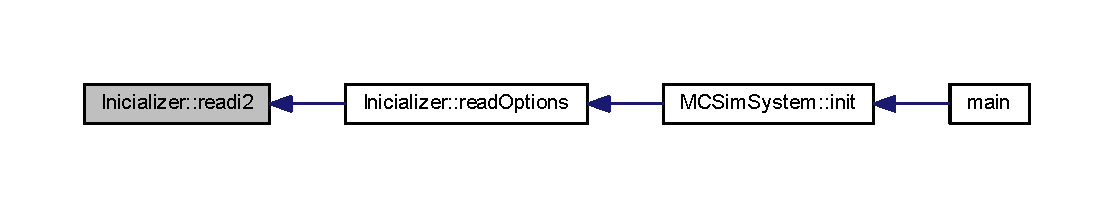
\includegraphics[width=350pt]{class_inicializer_ab20cbac5cc1211b24da005557a67ea10_icgraph}
\end{center}
\end{figure}


\hypertarget{class_inicializer_a59b1de21fff55d47d71f1e3f56a6b23f}{\index{Inicializer@{Inicializer}!readii2@{readii2}}
\index{readii2@{readii2}!Inicializer@{Inicializer}}
\subsubsection[{readii2}]{\setlength{\rightskip}{0pt plus 5cm}void Inicializer\+::readii2 (
\begin{DoxyParamCaption}
\item[{char $\ast$}]{num, }
\item[{int}]{value\mbox{[}2\mbox{]}}
\end{DoxyParamCaption}
)\hspace{0.3cm}{\ttfamily [private]}}}\label{class_inicializer_a59b1de21fff55d47d71f1e3f56a6b23f}


convert string num into two integers 


\begin{DoxyParams}{Parameters}
{\em num} & \\
\hline
{\em value} & \\
\hline
\end{DoxyParams}


Here is the call graph for this function\+:\nopagebreak
\begin{figure}[H]
\begin{center}
\leavevmode
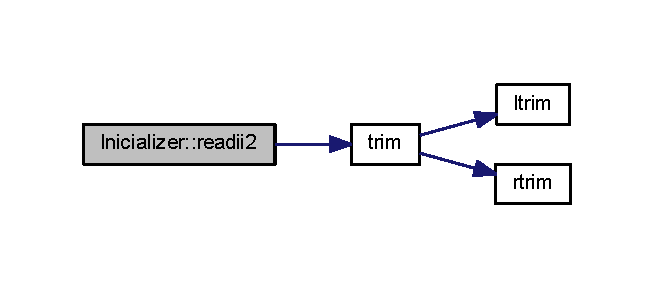
\includegraphics[width=314pt]{class_inicializer_a59b1de21fff55d47d71f1e3f56a6b23f_cgraph}
\end{center}
\end{figure}




Here is the caller graph for this function\+:\nopagebreak
\begin{figure}[H]
\begin{center}
\leavevmode
\includegraphics[width=350pt]{class_inicializer_a59b1de21fff55d47d71f1e3f56a6b23f_icgraph}
\end{center}
\end{figure}


\hypertarget{class_inicializer_added4b028cc3d6118d1b8c92c3eedd82}{\index{Inicializer@{Inicializer}!readl2@{readl2}}
\index{readl2@{readl2}!Inicializer@{Inicializer}}
\subsubsection[{readl2}]{\setlength{\rightskip}{0pt plus 5cm}long Inicializer\+::readl2 (
\begin{DoxyParamCaption}
\item[{char $\ast$}]{num}
\end{DoxyParamCaption}
)\hspace{0.3cm}{\ttfamily [private]}}}\label{class_inicializer_added4b028cc3d6118d1b8c92c3eedd82}


convert string num into long 


\begin{DoxyParams}{Parameters}
{\em num} & \\
\hline
\end{DoxyParams}
\begin{DoxyReturn}{Returns}

\end{DoxyReturn}


Here is the caller graph for this function\+:\nopagebreak
\begin{figure}[H]
\begin{center}
\leavevmode
\includegraphics[width=350pt]{class_inicializer_added4b028cc3d6118d1b8c92c3eedd82_icgraph}
\end{center}
\end{figure}


\hypertarget{class_inicializer_a41ac3793bca326b7b0d47c342bebf7b4}{\index{Inicializer@{Inicializer}!read\+Options@{read\+Options}}
\index{read\+Options@{read\+Options}!Inicializer@{Inicializer}}
\subsubsection[{read\+Options}]{\setlength{\rightskip}{0pt plus 5cm}void Inicializer\+::read\+Options (
\begin{DoxyParamCaption}
{}
\end{DoxyParamCaption}
)}}\label{class_inicializer_a41ac3793bca326b7b0d47c342bebf7b4}


Reads the run parameters from the external file \char`\"{}options\char`\"{}. See the end of the code for a template. All comments starting with '\#' are stripped out. The options are summarised on standard output and checked for validity of range. 



Here is the call graph for this function\+:\nopagebreak
\begin{figure}[H]
\begin{center}
\leavevmode
\includegraphics[width=350pt]{class_inicializer_a41ac3793bca326b7b0d47c342bebf7b4_cgraph}
\end{center}
\end{figure}




Here is the caller graph for this function\+:\nopagebreak
\begin{figure}[H]
\begin{center}
\leavevmode
\includegraphics[width=350pt]{class_inicializer_a41ac3793bca326b7b0d47c342bebf7b4_icgraph}
\end{center}
\end{figure}


\hypertarget{class_inicializer_acd2d40a23bdd29b973176c62ab5aef8d}{\index{Inicializer@{Inicializer}!read\+Topo\+File@{read\+Topo\+File}}
\index{read\+Topo\+File@{read\+Topo\+File}!Inicializer@{Inicializer}}
\subsubsection[{read\+Topo\+File}]{\setlength{\rightskip}{0pt plus 5cm}void Inicializer\+::read\+Topo\+File (
\begin{DoxyParamCaption}
\item[{{\bf Molecule} $\ast$}]{molecules, }
\item[{long $\ast$}]{sysmoln, }
\item[{char $\ast$}]{sysnames\mbox{[}$\,$\mbox{]}, }
\item[{bool}]{exclusions\mbox{[}$\,$\mbox{]}\mbox{[}\+M\+A\+X\+T\mbox{]}}
\end{DoxyParamCaption}
)\hspace{0.3cm}{\ttfamily [private]}}}\label{class_inicializer_acd2d40a23bdd29b973176c62ab5aef8d}


Here is the call graph for this function\+:\nopagebreak
\begin{figure}[H]
\begin{center}
\leavevmode
\includegraphics[width=350pt]{class_inicializer_acd2d40a23bdd29b973176c62ab5aef8d_cgraph}
\end{center}
\end{figure}




Here is the caller graph for this function\+:\nopagebreak
\begin{figure}[H]
\begin{center}
\leavevmode
\includegraphics[width=350pt]{class_inicializer_acd2d40a23bdd29b973176c62ab5aef8d_icgraph}
\end{center}
\end{figure}


\hypertarget{class_inicializer_a228deba06743d06562179c7f85b958ad}{\index{Inicializer@{Inicializer}!test\+Chains@{test\+Chains}}
\index{test\+Chains@{test\+Chains}!Inicializer@{Inicializer}}
\subsubsection[{test\+Chains}]{\setlength{\rightskip}{0pt plus 5cm}void Inicializer\+::test\+Chains (
\begin{DoxyParamCaption}
{}
\end{DoxyParamCaption}
)}}\label{class_inicializer_a228deba06743d06562179c7f85b958ad}


test if simulation contains Chains, sets probability of chain move to 0 if no chains 



Here is the caller graph for this function\+:\nopagebreak
\begin{figure}[H]
\begin{center}
\leavevmode
\includegraphics[width=350pt]{class_inicializer_a228deba06743d06562179c7f85b958ad_icgraph}
\end{center}
\end{figure}


\hypertarget{class_inicializer_a64fa047683e35560283287c30e269f9a}{\index{Inicializer@{Inicializer}!top\+Dealoc@{top\+Dealoc}}
\index{top\+Dealoc@{top\+Dealoc}!Inicializer@{Inicializer}}
\subsubsection[{top\+Dealoc}]{\setlength{\rightskip}{0pt plus 5cm}int Inicializer\+::top\+Dealoc (
\begin{DoxyParamCaption}
\item[{char $\ast$}]{sysnames\mbox{[}\+M\+A\+X\+N\mbox{]}, }
\item[{long $\ast$$\ast$}]{sysmoln, }
\item[{{\bf Molecule} $\ast$}]{molecules}
\end{DoxyParamCaption}
)\hspace{0.3cm}{\ttfamily [private]}}}\label{class_inicializer_a64fa047683e35560283287c30e269f9a}


dealocating memory for init\+Top 


\begin{DoxyParams}{Parameters}
{\em pline} & \\
\hline
{\em sysnames} & \\
\hline
{\em sysmoln} & \\
\hline
{\em molecules} & \\
\hline
\end{DoxyParams}
\begin{DoxyReturn}{Returns}

\end{DoxyReturn}


Here is the caller graph for this function\+:\nopagebreak
\begin{figure}[H]
\begin{center}
\leavevmode
\includegraphics[width=350pt]{class_inicializer_a64fa047683e35560283287c30e269f9a_icgraph}
\end{center}
\end{figure}


\hypertarget{class_inicializer_ac5d3d17ceb46d4096e173fa373bd12f6}{\index{Inicializer@{Inicializer}!use\+P\+B\+C@{use\+P\+B\+C}}
\index{use\+P\+B\+C@{use\+P\+B\+C}!Inicializer@{Inicializer}}
\subsubsection[{use\+P\+B\+C}]{\setlength{\rightskip}{0pt plus 5cm}void Inicializer\+::use\+P\+B\+C (
\begin{DoxyParamCaption}
\item[{{\bf Vector} $\ast$}]{pos, }
\item[{{\bf Vector}}]{pbc}
\end{DoxyParamCaption}
)\hspace{0.3cm}{\ttfamily [private]}}}\label{class_inicializer_ac5d3d17ceb46d4096e173fa373bd12f6}


use of periodic boundary conditions 


\begin{DoxyParams}{Parameters}
{\em pos} & \\
\hline
{\em pbc} & \\
\hline
\end{DoxyParams}


Here is the caller graph for this function\+:\nopagebreak
\begin{figure}[H]
\begin{center}
\leavevmode
\includegraphics[width=350pt]{class_inicializer_ac5d3d17ceb46d4096e173fa373bd12f6_icgraph}
\end{center}
\end{figure}


\hypertarget{class_inicializer_a271a0eef3110b4f1557c7b43d2e0320c}{\index{Inicializer@{Inicializer}!x\+Malloc@{x\+Malloc}}
\index{x\+Malloc@{x\+Malloc}!Inicializer@{Inicializer}}
\subsubsection[{x\+Malloc}]{\setlength{\rightskip}{0pt plus 5cm}void $\ast$ Inicializer\+::x\+Malloc (
\begin{DoxyParamCaption}
\item[{size\+\_\+t}]{num}
\end{DoxyParamCaption}
)\hspace{0.3cm}{\ttfamily [private]}}}\label{class_inicializer_a271a0eef3110b4f1557c7b43d2e0320c}


xmalloc nice malloc, which does the error checking for us 


\begin{DoxyParams}{Parameters}
{\em num} & \\
\hline
\end{DoxyParams}
\begin{DoxyReturn}{Returns}

\end{DoxyReturn}


\subsection{Member Data Documentation}
\hypertarget{class_inicializer_a6a3bb727f3ad6db5c667f615596cd5e4}{\index{Inicializer@{Inicializer}!conf@{conf}}
\index{conf@{conf}!Inicializer@{Inicializer}}
\subsubsection[{conf}]{\setlength{\rightskip}{0pt plus 5cm}{\bf Conf}$\ast$ Inicializer\+::conf\hspace{0.3cm}{\ttfamily [private]}}}\label{class_inicializer_a6a3bb727f3ad6db5c667f615596cd5e4}
\hypertarget{class_inicializer_aecd4b4dcea44e06dd58000db4144e93e}{\index{Inicializer@{Inicializer}!files@{files}}
\index{files@{files}!Inicializer@{Inicializer}}
\subsubsection[{files}]{\setlength{\rightskip}{0pt plus 5cm}{\bf File\+Names}$\ast$ Inicializer\+::files\hspace{0.3cm}{\ttfamily [private]}}}\label{class_inicializer_aecd4b4dcea44e06dd58000db4144e93e}
\hypertarget{class_inicializer_a98c446c361d34327e838a17737126212}{\index{Inicializer@{Inicializer}!seed@{seed}}
\index{seed@{seed}!Inicializer@{Inicializer}}
\subsubsection[{seed}]{\setlength{\rightskip}{0pt plus 5cm}long Inicializer\+::seed\hspace{0.3cm}{\ttfamily [private]}}}\label{class_inicializer_a98c446c361d34327e838a17737126212}
\hypertarget{class_inicializer_a8d55514c1121c5d3edbbd4fdfb32db65}{\index{Inicializer@{Inicializer}!sim@{sim}}
\index{sim@{sim}!Inicializer@{Inicializer}}
\subsubsection[{sim}]{\setlength{\rightskip}{0pt plus 5cm}{\bf Sim}$\ast$ Inicializer\+::sim\hspace{0.3cm}{\ttfamily [private]}}}\label{class_inicializer_a8d55514c1121c5d3edbbd4fdfb32db65}
\hypertarget{class_inicializer_a9ce346ffecd5ecf76bd4c1c68a3060f7}{\index{Inicializer@{Inicializer}!topo@{topo}}
\index{topo@{topo}!Inicializer@{Inicializer}}
\subsubsection[{topo}]{\setlength{\rightskip}{0pt plus 5cm}{\bf Topo}$\ast$ Inicializer\+::topo\hspace{0.3cm}{\ttfamily [private]}}}\label{class_inicializer_a9ce346ffecd5ecf76bd4c1c68a3060f7}


The documentation for this class was generated from the following files\+:\begin{DoxyCompactItemize}
\item 
sc\+O\+O\+P/mc/\hyperlink{inicializer_8h}{inicializer.\+h}\item 
sc\+O\+O\+P/mc/\hyperlink{inicializer_8cpp}{inicializer.\+cpp}\end{DoxyCompactItemize}

\hypertarget{class_m_c_sim_system}{\section{M\+C\+Sim\+System Class Reference}
\label{class_m_c_sim_system}\index{M\+C\+Sim\+System@{M\+C\+Sim\+System}}
}


{\ttfamily \#include $<$mcsimsystem.\+h$>$}



Collaboration diagram for M\+C\+Sim\+System\+:\nopagebreak
\begin{figure}[H]
\begin{center}
\leavevmode
\includegraphics[width=350pt]{class_m_c_sim_system__coll__graph}
\end{center}
\end{figure}
\subsection*{Public Member Functions}
\begin{DoxyCompactItemize}
\item 
\hyperlink{class_m_c_sim_system_ace11df1bb6f80f7654aa088870aa7271}{M\+C\+Sim\+System} ()
\item 
\hyperlink{class_m_c_sim_system_a6dd3f00bcb990de568515dcd65d26624}{$\sim$\+M\+C\+Sim\+System} ()
\item 
void \hyperlink{class_m_c_sim_system_adfacc1a896841b090ebab26fd369f43a}{init} ()
\begin{DoxyCompactList}\small\item\em init \end{DoxyCompactList}\item 
void \hyperlink{class_m_c_sim_system_a4f11a2356f82dba787e1a4d69e0e0d4f}{equilibrate} ()
\begin{DoxyCompactList}\small\item\em equilibrate \end{DoxyCompactList}\item 
void \hyperlink{class_m_c_sim_system_a188410921d582e9a2659627f4ca2073b}{production\+Run} ()
\begin{DoxyCompactList}\small\item\em production\+Run \end{DoxyCompactList}\item 
void \hyperlink{class_m_c_sim_system_a5886c6bfb00df9e66bf659673cd03854}{dealloc} ()
\begin{DoxyCompactList}\small\item\em dealloc \end{DoxyCompactList}\end{DoxyCompactItemize}
\subsection*{Private Member Functions}
\begin{DoxyCompactItemize}
\item 
void \hyperlink{class_m_c_sim_system_a6bf0bdd480a14c93b53177e32d502295}{clear\+Outfiles} ()
\begin{DoxyCompactList}\small\item\em clear\+Outfiles Clears outfiles for movie and Wang-\/\+Landau method \end{DoxyCompactList}\item 
int \hyperlink{class_m_c_sim_system_a780a1180f5bbe06b66ec672802f0a7b9}{memory\+Dealloc} ()
\begin{DoxyCompactList}\small\item\em memorydealloc \end{DoxyCompactList}\item 
int \hyperlink{class_m_c_sim_system_a5a4cc59839d79f6712f25bea5c5696d2}{dealloc\+Pairlist} ()
\begin{DoxyCompactList}\small\item\em dealloc\+\_\+pairlist Cleans up\+: deallocates the memory for the pairlist \end{DoxyCompactList}\end{DoxyCompactItemize}
\subsection*{Private Attributes}
\begin{DoxyCompactItemize}
\item 
F\+I\+L\+E $\ast$ \hyperlink{class_m_c_sim_system_afcf7ff09960e6fe9ebcd0af9d6ef5c77}{outfile}
\item 
F\+I\+L\+E $\ast$ \hyperlink{class_m_c_sim_system_af99ffcf84213091b20ff0e2e9c5fc0a4}{mov}
\item 
\hyperlink{struct_topo}{Topo} \hyperlink{class_m_c_sim_system_a27d68360d188e564c5b0e8991e63671c}{topo}
\item 
\hyperlink{struct_sim}{Sim} \hyperlink{class_m_c_sim_system_a157d4d5a003e91c72b954873e0a4593e}{sim}
\item 
\hyperlink{class_conf}{Conf} \hyperlink{class_m_c_sim_system_a4d6bf102d6233f299097ca228e1d5a1b}{conf}
\item 
\hyperlink{struct_file_names}{File\+Names} \hyperlink{class_m_c_sim_system_a251780d565abe7fe418ecd9ce0ba7aaa}{files}
\item 
\hyperlink{class_updater}{Updater} $\ast$ \hyperlink{class_m_c_sim_system_af7c8b2a6f211b0c6f8adc3f773f775f7}{updater}
\end{DoxyCompactItemize}


\subsection{Constructor \& Destructor Documentation}
\hypertarget{class_m_c_sim_system_ace11df1bb6f80f7654aa088870aa7271}{\index{M\+C\+Sim\+System@{M\+C\+Sim\+System}!M\+C\+Sim\+System@{M\+C\+Sim\+System}}
\index{M\+C\+Sim\+System@{M\+C\+Sim\+System}!M\+C\+Sim\+System@{M\+C\+Sim\+System}}
\subsubsection[{M\+C\+Sim\+System}]{\setlength{\rightskip}{0pt plus 5cm}M\+C\+Sim\+System\+::\+M\+C\+Sim\+System (
\begin{DoxyParamCaption}
{}
\end{DoxyParamCaption}
)\hspace{0.3cm}{\ttfamily [inline]}}}\label{class_m_c_sim_system_ace11df1bb6f80f7654aa088870aa7271}
\hypertarget{class_m_c_sim_system_a6dd3f00bcb990de568515dcd65d26624}{\index{M\+C\+Sim\+System@{M\+C\+Sim\+System}!````~M\+C\+Sim\+System@{$\sim$\+M\+C\+Sim\+System}}
\index{````~M\+C\+Sim\+System@{$\sim$\+M\+C\+Sim\+System}!M\+C\+Sim\+System@{M\+C\+Sim\+System}}
\subsubsection[{$\sim$\+M\+C\+Sim\+System}]{\setlength{\rightskip}{0pt plus 5cm}M\+C\+Sim\+System\+::$\sim$\+M\+C\+Sim\+System (
\begin{DoxyParamCaption}
{}
\end{DoxyParamCaption}
)\hspace{0.3cm}{\ttfamily [inline]}}}\label{class_m_c_sim_system_a6dd3f00bcb990de568515dcd65d26624}


\subsection{Member Function Documentation}
\hypertarget{class_m_c_sim_system_a6bf0bdd480a14c93b53177e32d502295}{\index{M\+C\+Sim\+System@{M\+C\+Sim\+System}!clear\+Outfiles@{clear\+Outfiles}}
\index{clear\+Outfiles@{clear\+Outfiles}!M\+C\+Sim\+System@{M\+C\+Sim\+System}}
\subsubsection[{clear\+Outfiles}]{\setlength{\rightskip}{0pt plus 5cm}void M\+C\+Sim\+System\+::clear\+Outfiles (
\begin{DoxyParamCaption}
{}
\end{DoxyParamCaption}
)\hspace{0.3cm}{\ttfamily [private]}}}\label{class_m_c_sim_system_a6bf0bdd480a14c93b53177e32d502295}


clear\+Outfiles Clears outfiles for movie and Wang-\/\+Landau method 



Here is the call graph for this function\+:\nopagebreak
\begin{figure}[H]
\begin{center}
\leavevmode
\includegraphics[width=350pt]{class_m_c_sim_system_a6bf0bdd480a14c93b53177e32d502295_cgraph}
\end{center}
\end{figure}




Here is the caller graph for this function\+:\nopagebreak
\begin{figure}[H]
\begin{center}
\leavevmode
\includegraphics[width=350pt]{class_m_c_sim_system_a6bf0bdd480a14c93b53177e32d502295_icgraph}
\end{center}
\end{figure}


\hypertarget{class_m_c_sim_system_a5886c6bfb00df9e66bf659673cd03854}{\index{M\+C\+Sim\+System@{M\+C\+Sim\+System}!dealloc@{dealloc}}
\index{dealloc@{dealloc}!M\+C\+Sim\+System@{M\+C\+Sim\+System}}
\subsubsection[{dealloc}]{\setlength{\rightskip}{0pt plus 5cm}void M\+C\+Sim\+System\+::dealloc (
\begin{DoxyParamCaption}
{}
\end{DoxyParamCaption}
)}}\label{class_m_c_sim_system_a5886c6bfb00df9e66bf659673cd03854}


dealloc 



Here is the call graph for this function\+:\nopagebreak
\begin{figure}[H]
\begin{center}
\leavevmode
\includegraphics[width=350pt]{class_m_c_sim_system_a5886c6bfb00df9e66bf659673cd03854_cgraph}
\end{center}
\end{figure}




Here is the caller graph for this function\+:\nopagebreak
\begin{figure}[H]
\begin{center}
\leavevmode
\includegraphics[width=274pt]{class_m_c_sim_system_a5886c6bfb00df9e66bf659673cd03854_icgraph}
\end{center}
\end{figure}


\hypertarget{class_m_c_sim_system_a5a4cc59839d79f6712f25bea5c5696d2}{\index{M\+C\+Sim\+System@{M\+C\+Sim\+System}!dealloc\+Pairlist@{dealloc\+Pairlist}}
\index{dealloc\+Pairlist@{dealloc\+Pairlist}!M\+C\+Sim\+System@{M\+C\+Sim\+System}}
\subsubsection[{dealloc\+Pairlist}]{\setlength{\rightskip}{0pt plus 5cm}int M\+C\+Sim\+System\+::dealloc\+Pairlist (
\begin{DoxyParamCaption}
{}
\end{DoxyParamCaption}
)\hspace{0.3cm}{\ttfamily [private]}}}\label{class_m_c_sim_system_a5a4cc59839d79f6712f25bea5c5696d2}


dealloc\+\_\+pairlist Cleans up\+: deallocates the memory for the pairlist 


\begin{DoxyParams}{Parameters}
{\em topo} & \\
\hline
{\em sim} & \\
\hline
\end{DoxyParams}
\begin{DoxyReturn}{Returns}

\end{DoxyReturn}


Here is the caller graph for this function\+:\nopagebreak
\begin{figure}[H]
\begin{center}
\leavevmode
\includegraphics[width=350pt]{class_m_c_sim_system_a5a4cc59839d79f6712f25bea5c5696d2_icgraph}
\end{center}
\end{figure}


\hypertarget{class_m_c_sim_system_a4f11a2356f82dba787e1a4d69e0e0d4f}{\index{M\+C\+Sim\+System@{M\+C\+Sim\+System}!equilibrate@{equilibrate}}
\index{equilibrate@{equilibrate}!M\+C\+Sim\+System@{M\+C\+Sim\+System}}
\subsubsection[{equilibrate}]{\setlength{\rightskip}{0pt plus 5cm}void M\+C\+Sim\+System\+::equilibrate (
\begin{DoxyParamCaption}
{}
\end{DoxyParamCaption}
)}}\label{class_m_c_sim_system_a4f11a2356f82dba787e1a4d69e0e0d4f}


equilibrate 



Here is the call graph for this function\+:
\nopagebreak
\begin{figure}[H]
\begin{center}
\leavevmode
\includegraphics[width=350pt]{class_m_c_sim_system_a4f11a2356f82dba787e1a4d69e0e0d4f_cgraph}
\end{center}
\end{figure}




Here is the caller graph for this function\+:\nopagebreak
\begin{figure}[H]
\begin{center}
\leavevmode
\includegraphics[width=288pt]{class_m_c_sim_system_a4f11a2356f82dba787e1a4d69e0e0d4f_icgraph}
\end{center}
\end{figure}


\hypertarget{class_m_c_sim_system_adfacc1a896841b090ebab26fd369f43a}{\index{M\+C\+Sim\+System@{M\+C\+Sim\+System}!init@{init}}
\index{init@{init}!M\+C\+Sim\+System@{M\+C\+Sim\+System}}
\subsubsection[{init}]{\setlength{\rightskip}{0pt plus 5cm}void M\+C\+Sim\+System\+::init (
\begin{DoxyParamCaption}
{}
\end{DoxyParamCaption}
)}}\label{class_m_c_sim_system_adfacc1a896841b090ebab26fd369f43a}


init 



Here is the call graph for this function\+:\nopagebreak
\begin{figure}[H]
\begin{center}
\leavevmode
\includegraphics[width=350pt]{class_m_c_sim_system_adfacc1a896841b090ebab26fd369f43a_cgraph}
\end{center}
\end{figure}




Here is the caller graph for this function\+:\nopagebreak
\begin{figure}[H]
\begin{center}
\leavevmode
\includegraphics[width=256pt]{class_m_c_sim_system_adfacc1a896841b090ebab26fd369f43a_icgraph}
\end{center}
\end{figure}


\hypertarget{class_m_c_sim_system_a780a1180f5bbe06b66ec672802f0a7b9}{\index{M\+C\+Sim\+System@{M\+C\+Sim\+System}!memory\+Dealloc@{memory\+Dealloc}}
\index{memory\+Dealloc@{memory\+Dealloc}!M\+C\+Sim\+System@{M\+C\+Sim\+System}}
\subsubsection[{memory\+Dealloc}]{\setlength{\rightskip}{0pt plus 5cm}int M\+C\+Sim\+System\+::memory\+Dealloc (
\begin{DoxyParamCaption}
{}
\end{DoxyParamCaption}
)\hspace{0.3cm}{\ttfamily [private]}}}\label{class_m_c_sim_system_a780a1180f5bbe06b66ec672802f0a7b9}


memorydealloc 



Here is the call graph for this function\+:\nopagebreak
\begin{figure}[H]
\begin{center}
\leavevmode
\includegraphics[width=350pt]{class_m_c_sim_system_a780a1180f5bbe06b66ec672802f0a7b9_cgraph}
\end{center}
\end{figure}




Here is the caller graph for this function\+:\nopagebreak
\begin{figure}[H]
\begin{center}
\leavevmode
\includegraphics[width=350pt]{class_m_c_sim_system_a780a1180f5bbe06b66ec672802f0a7b9_icgraph}
\end{center}
\end{figure}


\hypertarget{class_m_c_sim_system_a188410921d582e9a2659627f4ca2073b}{\index{M\+C\+Sim\+System@{M\+C\+Sim\+System}!production\+Run@{production\+Run}}
\index{production\+Run@{production\+Run}!M\+C\+Sim\+System@{M\+C\+Sim\+System}}
\subsubsection[{production\+Run}]{\setlength{\rightskip}{0pt plus 5cm}void M\+C\+Sim\+System\+::production\+Run (
\begin{DoxyParamCaption}
{}
\end{DoxyParamCaption}
)}}\label{class_m_c_sim_system_a188410921d582e9a2659627f4ca2073b}


production\+Run 

For testing the pairlist

For testing the cluster algorithm 

Here is the call graph for this function\+:
\nopagebreak
\begin{figure}[H]
\begin{center}
\leavevmode
\includegraphics[width=350pt]{class_m_c_sim_system_a188410921d582e9a2659627f4ca2073b_cgraph}
\end{center}
\end{figure}




Here is the caller graph for this function\+:\nopagebreak
\begin{figure}[H]
\begin{center}
\leavevmode
\includegraphics[width=306pt]{class_m_c_sim_system_a188410921d582e9a2659627f4ca2073b_icgraph}
\end{center}
\end{figure}




\subsection{Member Data Documentation}
\hypertarget{class_m_c_sim_system_a4d6bf102d6233f299097ca228e1d5a1b}{\index{M\+C\+Sim\+System@{M\+C\+Sim\+System}!conf@{conf}}
\index{conf@{conf}!M\+C\+Sim\+System@{M\+C\+Sim\+System}}
\subsubsection[{conf}]{\setlength{\rightskip}{0pt plus 5cm}{\bf Conf} M\+C\+Sim\+System\+::conf\hspace{0.3cm}{\ttfamily [private]}}}\label{class_m_c_sim_system_a4d6bf102d6233f299097ca228e1d5a1b}
\hypertarget{class_m_c_sim_system_a251780d565abe7fe418ecd9ce0ba7aaa}{\index{M\+C\+Sim\+System@{M\+C\+Sim\+System}!files@{files}}
\index{files@{files}!M\+C\+Sim\+System@{M\+C\+Sim\+System}}
\subsubsection[{files}]{\setlength{\rightskip}{0pt plus 5cm}{\bf File\+Names} M\+C\+Sim\+System\+::files\hspace{0.3cm}{\ttfamily [private]}}}\label{class_m_c_sim_system_a251780d565abe7fe418ecd9ce0ba7aaa}
\hypertarget{class_m_c_sim_system_af99ffcf84213091b20ff0e2e9c5fc0a4}{\index{M\+C\+Sim\+System@{M\+C\+Sim\+System}!mov@{mov}}
\index{mov@{mov}!M\+C\+Sim\+System@{M\+C\+Sim\+System}}
\subsubsection[{mov}]{\setlength{\rightskip}{0pt plus 5cm}F\+I\+L\+E $\ast$ M\+C\+Sim\+System\+::mov\hspace{0.3cm}{\ttfamily [private]}}}\label{class_m_c_sim_system_af99ffcf84213091b20ff0e2e9c5fc0a4}
\hypertarget{class_m_c_sim_system_afcf7ff09960e6fe9ebcd0af9d6ef5c77}{\index{M\+C\+Sim\+System@{M\+C\+Sim\+System}!outfile@{outfile}}
\index{outfile@{outfile}!M\+C\+Sim\+System@{M\+C\+Sim\+System}}
\subsubsection[{outfile}]{\setlength{\rightskip}{0pt plus 5cm}F\+I\+L\+E$\ast$ M\+C\+Sim\+System\+::outfile\hspace{0.3cm}{\ttfamily [private]}}}\label{class_m_c_sim_system_afcf7ff09960e6fe9ebcd0af9d6ef5c77}
\hypertarget{class_m_c_sim_system_a157d4d5a003e91c72b954873e0a4593e}{\index{M\+C\+Sim\+System@{M\+C\+Sim\+System}!sim@{sim}}
\index{sim@{sim}!M\+C\+Sim\+System@{M\+C\+Sim\+System}}
\subsubsection[{sim}]{\setlength{\rightskip}{0pt plus 5cm}{\bf Sim} M\+C\+Sim\+System\+::sim\hspace{0.3cm}{\ttfamily [private]}}}\label{class_m_c_sim_system_a157d4d5a003e91c72b954873e0a4593e}
\hypertarget{class_m_c_sim_system_a27d68360d188e564c5b0e8991e63671c}{\index{M\+C\+Sim\+System@{M\+C\+Sim\+System}!topo@{topo}}
\index{topo@{topo}!M\+C\+Sim\+System@{M\+C\+Sim\+System}}
\subsubsection[{topo}]{\setlength{\rightskip}{0pt plus 5cm}{\bf Topo} M\+C\+Sim\+System\+::topo\hspace{0.3cm}{\ttfamily [private]}}}\label{class_m_c_sim_system_a27d68360d188e564c5b0e8991e63671c}
\hypertarget{class_m_c_sim_system_af7c8b2a6f211b0c6f8adc3f773f775f7}{\index{M\+C\+Sim\+System@{M\+C\+Sim\+System}!updater@{updater}}
\index{updater@{updater}!M\+C\+Sim\+System@{M\+C\+Sim\+System}}
\subsubsection[{updater}]{\setlength{\rightskip}{0pt plus 5cm}{\bf Updater}$\ast$ M\+C\+Sim\+System\+::updater\hspace{0.3cm}{\ttfamily [private]}}}\label{class_m_c_sim_system_af7c8b2a6f211b0c6f8adc3f773f775f7}


The documentation for this class was generated from the following files\+:\begin{DoxyCompactItemize}
\item 
sc\+O\+O\+P/mc/\hyperlink{mcsimsystem_8h}{mcsimsystem.\+h}\item 
sc\+O\+O\+P/mc/\hyperlink{mcsimsystem_8cpp}{mcsimsystem.\+cpp}\end{DoxyCompactItemize}

\hypertarget{class_mesh}{\section{Mesh Class Reference}
\label{class_mesh}\index{Mesh@{Mesh}}
}


\hyperlink{class_mesh}{Mesh} for hole order parameter.  




{\ttfamily \#include $<$mesh.\+h$>$}



Collaboration diagram for Mesh\+:\nopagebreak
\begin{figure}[H]
\begin{center}
\leavevmode
\includegraphics[width=135pt]{class_mesh__coll__graph}
\end{center}
\end{figure}
\subsection*{Public Member Functions}
\begin{DoxyCompactItemize}
\item 
\hyperlink{class_mesh_a2af137f1571af89172b9c102302c416b}{Mesh} ()
\item 
void \hyperlink{class_mesh_add86daba06ee8291c7908f4a1d5070b6}{set\+Conf} (\hyperlink{class_conf}{Conf} $\ast$\hyperlink{class_mesh_aea779b6c0ade9b15e724306f0a4652de}{conf})
\item 
int \hyperlink{class_mesh_a086d2a79604a0636b39d4d07c516867e}{mesh\+Init} (double meshsize, long npart, int wlmtype)
\begin{DoxyCompactList}\small\item\em mesh\+Init \end{DoxyCompactList}\item 
void \hyperlink{class_mesh_a287954614a974377a6adba50692158b8}{mesh\+Fill} (long npart, int wlmtype)
\begin{DoxyCompactList}\small\item\em filling the mesh \end{DoxyCompactList}\item 
int \hyperlink{class_mesh_ae1c06bc8b428ea8d854513b4ccf120cd}{find\+Holes} ()
\begin{DoxyCompactList}\small\item\em mesh\+\_\+findholes returns the number of holes and a list of mesh points belonging to each of them \end{DoxyCompactList}\item 
int \hyperlink{class_mesh_af373f0167a41061f4aa0f2741cb02da0}{find\+Holes\+Distrib} ()
\begin{DoxyCompactList}\small\item\em mesh\+\_\+findholesdistrib prints out distribution of holes and returns the number of holes and a list of mesh points belonging to each of them \end{DoxyCompactList}\item 
void \hyperlink{class_mesh_af5a35e846fe102b2b2c0232baf83f6cf}{print} ()
\begin{DoxyCompactList}\small\item\em mesh\+\_\+print \end{DoxyCompactList}\item 
void \hyperlink{class_mesh_a0c233a05716e43a7014f6346cc79d118}{operator=} (\hyperlink{class_mesh}{Mesh} \&source)
\begin{DoxyCompactList}\small\item\em mesh\+\_\+cpy \end{DoxyCompactList}\item 
int \hyperlink{class_mesh_a43ba112d0301e5e8dd9ccc31c2e2db86}{end} ()
\begin{DoxyCompactList}\small\item\em mesh\+\_\+end \end{DoxyCompactList}\end{DoxyCompactItemize}
\subsection*{Static Public Member Functions}
\begin{DoxyCompactItemize}
\item 
static int \hyperlink{class_mesh_a3779de5e24f96ab307153f3ab3cb67b0}{add\+Part} (double posx, double posy, int $\ast$$\ast$mesh, int \hyperlink{class_mesh_a634550923b75db84904c094677bd415e}{dim}\mbox{[}2\mbox{]})
\begin{DoxyCompactList}\small\item\em mesh\+\_\+addpart add particle on coordinates posx posy to mesh return 0 if it was placed on empty spot \end{DoxyCompactList}\item 
static int \hyperlink{class_mesh_afff05228d5e595d978f39ace32a8aea6}{remove\+Part} (double posx, double posy, int $\ast$$\ast$mesh, int \hyperlink{class_mesh_a634550923b75db84904c094677bd415e}{dim}\mbox{[}2\mbox{]})
\begin{DoxyCompactList}\small\item\em mesh\+\_\+removepart remove particle on coordinates posx posy from mesh and return 0 if there is a empty spot now \end{DoxyCompactList}\item 
static void \hyperlink{class_mesh_a824270e8af4d5eb1b93a55cc5541fb38}{mesh\+Square} (int x, int y, int \hyperlink{class_mesh_a634550923b75db84904c094677bd415e}{dim}\mbox{[}2\mbox{]}, int($\ast$square)\mbox{[}9\mbox{]})
\begin{DoxyCompactList}\small\item\em mesh\+\_\+square \end{DoxyCompactList}\item 
static void \hyperlink{class_mesh_aec76a31895c9092b5f0528a73f100d1c}{mesh\+Neighbors} (int pos, int \hyperlink{class_mesh_a634550923b75db84904c094677bd415e}{dim}\mbox{[}2\mbox{]}, int neighbors\mbox{[}4\mbox{]})
\begin{DoxyCompactList}\small\item\em mesh\+\_\+neighbors \end{DoxyCompactList}\end{DoxyCompactItemize}
\subsection*{Public Attributes}
\begin{DoxyCompactItemize}
\item 
int \hyperlink{class_mesh_a634550923b75db84904c094677bd415e}{dim} \mbox{[}2\mbox{]}
\begin{DoxyCompactList}\small\item\em \hyperlink{class_mesh}{Mesh} dimensions. \end{DoxyCompactList}\item 
int $\ast$ \hyperlink{class_mesh_a00e5cec14c115343cc6e4b6769c5a3b3}{data}
\begin{DoxyCompactList}\small\item\em \hyperlink{class_mesh}{Mesh} data. \end{DoxyCompactList}\item 
int $\ast$ \hyperlink{class_mesh_a2f5a473ab6b6f76d3dd1f2886d0da89d}{tmp}
\begin{DoxyCompactList}\small\item\em tempporary list for hole search \end{DoxyCompactList}\end{DoxyCompactItemize}
\subsection*{Private Attributes}
\begin{DoxyCompactItemize}
\item 
\hyperlink{class_conf}{Conf} $\ast$ \hyperlink{class_mesh_aea779b6c0ade9b15e724306f0a4652de}{conf}
\end{DoxyCompactItemize}


\subsection{Detailed Description}
\hyperlink{class_mesh}{Mesh} for hole order parameter. 

\subsection{Constructor \& Destructor Documentation}
\hypertarget{class_mesh_a2af137f1571af89172b9c102302c416b}{\index{Mesh@{Mesh}!Mesh@{Mesh}}
\index{Mesh@{Mesh}!Mesh@{Mesh}}
\subsubsection[{Mesh}]{\setlength{\rightskip}{0pt plus 5cm}Mesh\+::\+Mesh (
\begin{DoxyParamCaption}
{}
\end{DoxyParamCaption}
)\hspace{0.3cm}{\ttfamily [inline]}}}\label{class_mesh_a2af137f1571af89172b9c102302c416b}


\subsection{Member Function Documentation}
\hypertarget{class_mesh_a3779de5e24f96ab307153f3ab3cb67b0}{\index{Mesh@{Mesh}!add\+Part@{add\+Part}}
\index{add\+Part@{add\+Part}!Mesh@{Mesh}}
\subsubsection[{add\+Part}]{\setlength{\rightskip}{0pt plus 5cm}int Mesh\+::add\+Part (
\begin{DoxyParamCaption}
\item[{double}]{posx, }
\item[{double}]{posy, }
\item[{int $\ast$$\ast$}]{mesh, }
\item[{int}]{dim\mbox{[}2\mbox{]}}
\end{DoxyParamCaption}
)\hspace{0.3cm}{\ttfamily [static]}}}\label{class_mesh_a3779de5e24f96ab307153f3ab3cb67b0}


mesh\+\_\+addpart add particle on coordinates posx posy to mesh return 0 if it was placed on empty spot 


\begin{DoxyParams}{Parameters}
{\em posx} & \\
\hline
{\em posy} & \\
\hline
{\em mesh} & \\
\hline
{\em dim} & \\
\hline
\end{DoxyParams}
\begin{DoxyReturn}{Returns}

\end{DoxyReturn}


Here is the call graph for this function\+:\nopagebreak
\begin{figure}[H]
\begin{center}
\leavevmode
\includegraphics[width=298pt]{class_mesh_a3779de5e24f96ab307153f3ab3cb67b0_cgraph}
\end{center}
\end{figure}




Here is the caller graph for this function\+:\nopagebreak
\begin{figure}[H]
\begin{center}
\leavevmode
\includegraphics[width=350pt]{class_mesh_a3779de5e24f96ab307153f3ab3cb67b0_icgraph}
\end{center}
\end{figure}


\hypertarget{class_mesh_a43ba112d0301e5e8dd9ccc31c2e2db86}{\index{Mesh@{Mesh}!end@{end}}
\index{end@{end}!Mesh@{Mesh}}
\subsubsection[{end}]{\setlength{\rightskip}{0pt plus 5cm}int Mesh\+::end (
\begin{DoxyParamCaption}
{}
\end{DoxyParamCaption}
)}}\label{class_mesh_a43ba112d0301e5e8dd9ccc31c2e2db86}


mesh\+\_\+end 

\begin{DoxyReturn}{Returns}

\end{DoxyReturn}


Here is the caller graph for this function\+:\nopagebreak
\begin{figure}[H]
\begin{center}
\leavevmode
\includegraphics[width=350pt]{class_mesh_a43ba112d0301e5e8dd9ccc31c2e2db86_icgraph}
\end{center}
\end{figure}


\hypertarget{class_mesh_ae1c06bc8b428ea8d854513b4ccf120cd}{\index{Mesh@{Mesh}!find\+Holes@{find\+Holes}}
\index{find\+Holes@{find\+Holes}!Mesh@{Mesh}}
\subsubsection[{find\+Holes}]{\setlength{\rightskip}{0pt plus 5cm}int Mesh\+::find\+Holes (
\begin{DoxyParamCaption}
{}
\end{DoxyParamCaption}
)}}\label{class_mesh_ae1c06bc8b428ea8d854513b4ccf120cd}


mesh\+\_\+findholes returns the number of holes and a list of mesh points belonging to each of them 

\begin{DoxyReturn}{Returns}

\end{DoxyReturn}


Here is the call graph for this function\+:\nopagebreak
\begin{figure}[H]
\begin{center}
\leavevmode
\includegraphics[width=316pt]{class_mesh_ae1c06bc8b428ea8d854513b4ccf120cd_cgraph}
\end{center}
\end{figure}




Here is the caller graph for this function\+:\nopagebreak
\begin{figure}[H]
\begin{center}
\leavevmode
\includegraphics[width=350pt]{class_mesh_ae1c06bc8b428ea8d854513b4ccf120cd_icgraph}
\end{center}
\end{figure}


\hypertarget{class_mesh_af373f0167a41061f4aa0f2741cb02da0}{\index{Mesh@{Mesh}!find\+Holes\+Distrib@{find\+Holes\+Distrib}}
\index{find\+Holes\+Distrib@{find\+Holes\+Distrib}!Mesh@{Mesh}}
\subsubsection[{find\+Holes\+Distrib}]{\setlength{\rightskip}{0pt plus 5cm}int Mesh\+::find\+Holes\+Distrib (
\begin{DoxyParamCaption}
{}
\end{DoxyParamCaption}
)}}\label{class_mesh_af373f0167a41061f4aa0f2741cb02da0}


mesh\+\_\+findholesdistrib prints out distribution of holes and returns the number of holes and a list of mesh points belonging to each of them 

\begin{DoxyReturn}{Returns}

\end{DoxyReturn}
\hypertarget{class_mesh_a287954614a974377a6adba50692158b8}{\index{Mesh@{Mesh}!mesh\+Fill@{mesh\+Fill}}
\index{mesh\+Fill@{mesh\+Fill}!Mesh@{Mesh}}
\subsubsection[{mesh\+Fill}]{\setlength{\rightskip}{0pt plus 5cm}void Mesh\+::mesh\+Fill (
\begin{DoxyParamCaption}
\item[{long}]{npart, }
\item[{int}]{wlmtype}
\end{DoxyParamCaption}
)}}\label{class_mesh_a287954614a974377a6adba50692158b8}


filling the mesh 


\begin{DoxyParams}{Parameters}
{\em npart} & \\
\hline
{\em wlmtype} & \\
\hline
\end{DoxyParams}


Here is the call graph for this function\+:\nopagebreak
\begin{figure}[H]
\begin{center}
\leavevmode
\includegraphics[width=350pt]{class_mesh_a287954614a974377a6adba50692158b8_cgraph}
\end{center}
\end{figure}




Here is the caller graph for this function\+:\nopagebreak
\begin{figure}[H]
\begin{center}
\leavevmode
\includegraphics[width=350pt]{class_mesh_a287954614a974377a6adba50692158b8_icgraph}
\end{center}
\end{figure}


\hypertarget{class_mesh_a086d2a79604a0636b39d4d07c516867e}{\index{Mesh@{Mesh}!mesh\+Init@{mesh\+Init}}
\index{mesh\+Init@{mesh\+Init}!Mesh@{Mesh}}
\subsubsection[{mesh\+Init}]{\setlength{\rightskip}{0pt plus 5cm}int Mesh\+::mesh\+Init (
\begin{DoxyParamCaption}
\item[{double}]{meshsize, }
\item[{long}]{npart, }
\item[{int}]{wlmtype}
\end{DoxyParamCaption}
)}}\label{class_mesh_a086d2a79604a0636b39d4d07c516867e}


mesh\+Init 


\begin{DoxyParams}{Parameters}
{\em meshsize} & \\
\hline
{\em npart} & \\
\hline
{\em wlmtype} & \\
\hline
\end{DoxyParams}
\begin{DoxyReturn}{Returns}

\end{DoxyReturn}


Here is the call graph for this function\+:\nopagebreak
\begin{figure}[H]
\begin{center}
\leavevmode
\includegraphics[width=350pt]{class_mesh_a086d2a79604a0636b39d4d07c516867e_cgraph}
\end{center}
\end{figure}




Here is the caller graph for this function\+:\nopagebreak
\begin{figure}[H]
\begin{center}
\leavevmode
\includegraphics[width=350pt]{class_mesh_a086d2a79604a0636b39d4d07c516867e_icgraph}
\end{center}
\end{figure}


\hypertarget{class_mesh_aec76a31895c9092b5f0528a73f100d1c}{\index{Mesh@{Mesh}!mesh\+Neighbors@{mesh\+Neighbors}}
\index{mesh\+Neighbors@{mesh\+Neighbors}!Mesh@{Mesh}}
\subsubsection[{mesh\+Neighbors}]{\setlength{\rightskip}{0pt plus 5cm}void Mesh\+::mesh\+Neighbors (
\begin{DoxyParamCaption}
\item[{int}]{pos, }
\item[{int}]{dim\mbox{[}2\mbox{]}, }
\item[{int}]{neighbors\mbox{[}4\mbox{]}}
\end{DoxyParamCaption}
)\hspace{0.3cm}{\ttfamily [static]}}}\label{class_mesh_aec76a31895c9092b5f0528a73f100d1c}


mesh\+\_\+neighbors 


\begin{DoxyParams}{Parameters}
{\em pos} & \\
\hline
{\em dim} & \\
\hline
{\em neighbors} & \\
\hline
\end{DoxyParams}


Here is the caller graph for this function\+:\nopagebreak
\begin{figure}[H]
\begin{center}
\leavevmode
\includegraphics[width=350pt]{class_mesh_aec76a31895c9092b5f0528a73f100d1c_icgraph}
\end{center}
\end{figure}


\hypertarget{class_mesh_a824270e8af4d5eb1b93a55cc5541fb38}{\index{Mesh@{Mesh}!mesh\+Square@{mesh\+Square}}
\index{mesh\+Square@{mesh\+Square}!Mesh@{Mesh}}
\subsubsection[{mesh\+Square}]{\setlength{\rightskip}{0pt plus 5cm}void Mesh\+::mesh\+Square (
\begin{DoxyParamCaption}
\item[{int}]{x, }
\item[{int}]{y, }
\item[{int}]{dim\mbox{[}2\mbox{]}, }
\item[{int($\ast$)}]{square\mbox{[}9\mbox{]}}
\end{DoxyParamCaption}
)\hspace{0.3cm}{\ttfamily [static]}}}\label{class_mesh_a824270e8af4d5eb1b93a55cc5541fb38}


mesh\+\_\+square 


\begin{DoxyParams}{Parameters}
{\em x} & \\
\hline
{\em y} & \\
\hline
{\em dim} & \\
\hline
\end{DoxyParams}


Here is the caller graph for this function\+:\nopagebreak
\begin{figure}[H]
\begin{center}
\leavevmode
\includegraphics[width=350pt]{class_mesh_a824270e8af4d5eb1b93a55cc5541fb38_icgraph}
\end{center}
\end{figure}


\hypertarget{class_mesh_a0c233a05716e43a7014f6346cc79d118}{\index{Mesh@{Mesh}!operator=@{operator=}}
\index{operator=@{operator=}!Mesh@{Mesh}}
\subsubsection[{operator=}]{\setlength{\rightskip}{0pt plus 5cm}void Mesh\+::operator= (
\begin{DoxyParamCaption}
\item[{{\bf Mesh} \&}]{source}
\end{DoxyParamCaption}
)}}\label{class_mesh_a0c233a05716e43a7014f6346cc79d118}


mesh\+\_\+cpy 


\begin{DoxyParams}{Parameters}
{\em source} & \\
\hline
\end{DoxyParams}
\hypertarget{class_mesh_af5a35e846fe102b2b2c0232baf83f6cf}{\index{Mesh@{Mesh}!print@{print}}
\index{print@{print}!Mesh@{Mesh}}
\subsubsection[{print}]{\setlength{\rightskip}{0pt plus 5cm}void Mesh\+::print (
\begin{DoxyParamCaption}
{}
\end{DoxyParamCaption}
)}}\label{class_mesh_af5a35e846fe102b2b2c0232baf83f6cf}


mesh\+\_\+print 



Here is the call graph for this function\+:\nopagebreak
\begin{figure}[H]
\begin{center}
\leavevmode
\includegraphics[width=350pt]{class_mesh_af5a35e846fe102b2b2c0232baf83f6cf_cgraph}
\end{center}
\end{figure}


\hypertarget{class_mesh_afff05228d5e595d978f39ace32a8aea6}{\index{Mesh@{Mesh}!remove\+Part@{remove\+Part}}
\index{remove\+Part@{remove\+Part}!Mesh@{Mesh}}
\subsubsection[{remove\+Part}]{\setlength{\rightskip}{0pt plus 5cm}int Mesh\+::remove\+Part (
\begin{DoxyParamCaption}
\item[{double}]{posx, }
\item[{double}]{posy, }
\item[{int $\ast$$\ast$}]{mesh, }
\item[{int}]{dim\mbox{[}2\mbox{]}}
\end{DoxyParamCaption}
)\hspace{0.3cm}{\ttfamily [static]}}}\label{class_mesh_afff05228d5e595d978f39ace32a8aea6}


mesh\+\_\+removepart remove particle on coordinates posx posy from mesh and return 0 if there is a empty spot now 


\begin{DoxyParams}{Parameters}
{\em posx} & \\
\hline
{\em posy} & \\
\hline
{\em mesh} & \\
\hline
{\em dim} & \\
\hline
\end{DoxyParams}
\begin{DoxyReturn}{Returns}

\end{DoxyReturn}


Here is the call graph for this function\+:\nopagebreak
\begin{figure}[H]
\begin{center}
\leavevmode
\includegraphics[width=314pt]{class_mesh_afff05228d5e595d978f39ace32a8aea6_cgraph}
\end{center}
\end{figure}




Here is the caller graph for this function\+:\nopagebreak
\begin{figure}[H]
\begin{center}
\leavevmode
\includegraphics[width=350pt]{class_mesh_afff05228d5e595d978f39ace32a8aea6_icgraph}
\end{center}
\end{figure}


\hypertarget{class_mesh_add86daba06ee8291c7908f4a1d5070b6}{\index{Mesh@{Mesh}!set\+Conf@{set\+Conf}}
\index{set\+Conf@{set\+Conf}!Mesh@{Mesh}}
\subsubsection[{set\+Conf}]{\setlength{\rightskip}{0pt plus 5cm}void Mesh\+::set\+Conf (
\begin{DoxyParamCaption}
\item[{{\bf Conf} $\ast$}]{conf}
\end{DoxyParamCaption}
)\hspace{0.3cm}{\ttfamily [inline]}}}\label{class_mesh_add86daba06ee8291c7908f4a1d5070b6}


\subsection{Member Data Documentation}
\hypertarget{class_mesh_aea779b6c0ade9b15e724306f0a4652de}{\index{Mesh@{Mesh}!conf@{conf}}
\index{conf@{conf}!Mesh@{Mesh}}
\subsubsection[{conf}]{\setlength{\rightskip}{0pt plus 5cm}{\bf Conf}$\ast$ Mesh\+::conf\hspace{0.3cm}{\ttfamily [private]}}}\label{class_mesh_aea779b6c0ade9b15e724306f0a4652de}
\hypertarget{class_mesh_a00e5cec14c115343cc6e4b6769c5a3b3}{\index{Mesh@{Mesh}!data@{data}}
\index{data@{data}!Mesh@{Mesh}}
\subsubsection[{data}]{\setlength{\rightskip}{0pt plus 5cm}int$\ast$ Mesh\+::data}}\label{class_mesh_a00e5cec14c115343cc6e4b6769c5a3b3}


\hyperlink{class_mesh}{Mesh} data. 

\hypertarget{class_mesh_a634550923b75db84904c094677bd415e}{\index{Mesh@{Mesh}!dim@{dim}}
\index{dim@{dim}!Mesh@{Mesh}}
\subsubsection[{dim}]{\setlength{\rightskip}{0pt plus 5cm}int Mesh\+::dim\mbox{[}2\mbox{]}}}\label{class_mesh_a634550923b75db84904c094677bd415e}


\hyperlink{class_mesh}{Mesh} dimensions. 

\hypertarget{class_mesh_a2f5a473ab6b6f76d3dd1f2886d0da89d}{\index{Mesh@{Mesh}!tmp@{tmp}}
\index{tmp@{tmp}!Mesh@{Mesh}}
\subsubsection[{tmp}]{\setlength{\rightskip}{0pt plus 5cm}int$\ast$ Mesh\+::tmp}}\label{class_mesh_a2f5a473ab6b6f76d3dd1f2886d0da89d}


tempporary list for hole search 



The documentation for this class was generated from the following files\+:\begin{DoxyCompactItemize}
\item 
sc\+O\+O\+P/mc/\hyperlink{mesh_8h}{mesh.\+h}\item 
sc\+O\+O\+P/mc/\hyperlink{mesh_8cpp}{mesh.\+cpp}\end{DoxyCompactItemize}

\hypertarget{class_molecule}{\section{Molecule Class Reference}
\label{class_molecule}\index{Molecule@{Molecule}}
}


This structure is for io only.  




{\ttfamily \#include $<$structures.\+h$>$}

\subsection*{Public Member Functions}
\begin{DoxyCompactItemize}
\item 
\hyperlink{class_molecule_a7e7d290ae641518ad4c4d5303b519d0f}{Molecule} ()
\item 
\hyperlink{class_molecule_a1ff980b574a62526abff3d631c83bf94}{$\sim$\+Molecule} ()
\end{DoxyCompactItemize}
\subsection*{Public Attributes}
\begin{DoxyCompactItemize}
\item 
char $\ast$ \hyperlink{class_molecule_a905da45fb2ad1c821b7cf03c655c3047}{name}
\begin{DoxyCompactList}\small\item\em The name of the molecule. \end{DoxyCompactList}\item 
int $\ast$ \hyperlink{class_molecule_aa968965732a78fc8b2b60fc27d6374b6}{type}
\begin{DoxyCompactList}\small\item\em The type of the particle. \end{DoxyCompactList}\item 
long $\ast$ \hyperlink{class_molecule_acf6cf0f43a015cff8dde7970e1ca3abd}{switchtype}
\begin{DoxyCompactList}\small\item\em The switchtype of the particle. \end{DoxyCompactList}\item 
double $\ast$ \hyperlink{class_molecule_a6fd83a87d28a34e7098dc9d9f22b6c41}{delta\+\_\+mu}
\begin{DoxyCompactList}\small\item\em The chemical potential for the switch. \end{DoxyCompactList}\end{DoxyCompactItemize}


\subsection{Detailed Description}
This structure is for io only. 

\subsection{Constructor \& Destructor Documentation}
\hypertarget{class_molecule_a7e7d290ae641518ad4c4d5303b519d0f}{\index{Molecule@{Molecule}!Molecule@{Molecule}}
\index{Molecule@{Molecule}!Molecule@{Molecule}}
\subsubsection[{Molecule}]{\setlength{\rightskip}{0pt plus 5cm}Molecule\+::\+Molecule (
\begin{DoxyParamCaption}
{}
\end{DoxyParamCaption}
)\hspace{0.3cm}{\ttfamily [inline]}}}\label{class_molecule_a7e7d290ae641518ad4c4d5303b519d0f}
\hypertarget{class_molecule_a1ff980b574a62526abff3d631c83bf94}{\index{Molecule@{Molecule}!````~Molecule@{$\sim$\+Molecule}}
\index{````~Molecule@{$\sim$\+Molecule}!Molecule@{Molecule}}
\subsubsection[{$\sim$\+Molecule}]{\setlength{\rightskip}{0pt plus 5cm}Molecule\+::$\sim$\+Molecule (
\begin{DoxyParamCaption}
{}
\end{DoxyParamCaption}
)\hspace{0.3cm}{\ttfamily [inline]}}}\label{class_molecule_a1ff980b574a62526abff3d631c83bf94}


\subsection{Member Data Documentation}
\hypertarget{class_molecule_a6fd83a87d28a34e7098dc9d9f22b6c41}{\index{Molecule@{Molecule}!delta\+\_\+mu@{delta\+\_\+mu}}
\index{delta\+\_\+mu@{delta\+\_\+mu}!Molecule@{Molecule}}
\subsubsection[{delta\+\_\+mu}]{\setlength{\rightskip}{0pt plus 5cm}double$\ast$ Molecule\+::delta\+\_\+mu}}\label{class_molecule_a6fd83a87d28a34e7098dc9d9f22b6c41}


The chemical potential for the switch. 

\hypertarget{class_molecule_a905da45fb2ad1c821b7cf03c655c3047}{\index{Molecule@{Molecule}!name@{name}}
\index{name@{name}!Molecule@{Molecule}}
\subsubsection[{name}]{\setlength{\rightskip}{0pt plus 5cm}char$\ast$ Molecule\+::name}}\label{class_molecule_a905da45fb2ad1c821b7cf03c655c3047}


The name of the molecule. 

\hypertarget{class_molecule_acf6cf0f43a015cff8dde7970e1ca3abd}{\index{Molecule@{Molecule}!switchtype@{switchtype}}
\index{switchtype@{switchtype}!Molecule@{Molecule}}
\subsubsection[{switchtype}]{\setlength{\rightskip}{0pt plus 5cm}long$\ast$ Molecule\+::switchtype}}\label{class_molecule_acf6cf0f43a015cff8dde7970e1ca3abd}


The switchtype of the particle. 

\hypertarget{class_molecule_aa968965732a78fc8b2b60fc27d6374b6}{\index{Molecule@{Molecule}!type@{type}}
\index{type@{type}!Molecule@{Molecule}}
\subsubsection[{type}]{\setlength{\rightskip}{0pt plus 5cm}int$\ast$ Molecule\+::type}}\label{class_molecule_aa968965732a78fc8b2b60fc27d6374b6}


The type of the particle. 



The documentation for this class was generated from the following file\+:\begin{DoxyCompactItemize}
\item 
sc\+O\+O\+P/structures/\hyperlink{structures_8h}{structures.\+h}\end{DoxyCompactItemize}

\hypertarget{class_molecule_params}{\section{Molecule\+Params Class Reference}
\label{class_molecule_params}\index{Molecule\+Params@{Molecule\+Params}}
}


Parameters for inner interaction in chains.  




{\ttfamily \#include $<$moleculeparams.\+h$>$}

\subsection*{Public Member Functions}
\begin{DoxyCompactItemize}
\item 
\hyperlink{class_molecule_params_a33689bb37655eed3447e989be5149cf3}{Molecule\+Params} ()
\item 
bool \hyperlink{class_molecule_params_a4144cbf276e3e7e25c7a6f3557e4f80b}{is\+Atomic} ()
\item 
int \hyperlink{class_molecule_params_a025ace7f9070a6b19b7b536e1d7f565f}{mol\+Size} ()
\end{DoxyCompactItemize}
\subsection*{Public Attributes}
\begin{DoxyCompactItemize}
\item 
char $\ast$ \hyperlink{class_molecule_params_a9b478628f7e50569a41fdfb6dacfabfa}{name}
\begin{DoxyCompactList}\small\item\em name of the molecule \end{DoxyCompactList}\item 
double \hyperlink{class_molecule_params_af3ba3ec166a3d31ce27c707679dd7335}{bond1eq}
\begin{DoxyCompactList}\small\item\em Equilibrium distance of harmonic bond between nearest neighbours. \end{DoxyCompactList}\item 
double \hyperlink{class_molecule_params_a48d2ea6681c8eb398d74610cffab8594}{bond1c}
\begin{DoxyCompactList}\small\item\em Spring constant for harmonic bond between nearest neighbours. \end{DoxyCompactList}\item 
double \hyperlink{class_molecule_params_a7ba670c7097cbef3dbbaaf995f726f7e}{bond2eq}
\begin{DoxyCompactList}\small\item\em Equilibrium distance of harmonic bond between second nearest neighbours. \end{DoxyCompactList}\item 
double \hyperlink{class_molecule_params_a69fcc0cfc455c73f910b379860900a16}{bond2c}
\begin{DoxyCompactList}\small\item\em Spring constant for harmonic bond between second nearest neighbours. \end{DoxyCompactList}\item 
double \hyperlink{class_molecule_params_a55f6fb3edc8ca69966b06a6370f5c5c0}{bonddeq}
\begin{DoxyCompactList}\small\item\em Equilibrium distance of directional harmonic bond between the nearest neighbours. \end{DoxyCompactList}\item 
double \hyperlink{class_molecule_params_ae2c76f8dd300d5f70dbd905fea428e59}{bonddc}
\begin{DoxyCompactList}\small\item\em Spring constant for directional harmonic bond between the nearest neighbours. \end{DoxyCompactList}\item 
double \hyperlink{class_molecule_params_aa3a3e60ad09927ad74fce4eb8dbd2a91}{angle1eq}
\begin{DoxyCompactList}\small\item\em Equilibrium angle between two spherocylinders -\/neerest neighbours. \end{DoxyCompactList}\item 
double \hyperlink{class_molecule_params_a01cf1bc0ed829aeca3c1756af5c11841}{angle1c}
\begin{DoxyCompactList}\small\item\em Spring constant angle between two spherocylinders -\/nearest neighbours. \end{DoxyCompactList}\item 
double \hyperlink{class_molecule_params_aba6d4b6e5b9ee2d21f42046d2035b707}{angle2eq}
\begin{DoxyCompactList}\small\item\em Equilibrium angle between two spherocylinder patches -\/nearest neighbours. \end{DoxyCompactList}\item 
double \hyperlink{class_molecule_params_ac5666492fbac2859faf78bd7c5a1afc7}{angle2c}
\begin{DoxyCompactList}\small\item\em Spring constant for angle between two spherocylinder patches -\/nearest neighbours. \end{DoxyCompactList}\item 
double \hyperlink{class_molecule_params_a8155e1f14baf8e128df56a9a71f77de4}{mu}
\begin{DoxyCompactList}\small\item\em chemical potential, specific to each molecule type \end{DoxyCompactList}\item 
double \hyperlink{class_molecule_params_af02735d94bf97e0315d370a1d2dbc675}{ln\+Thermal\+Wavelengh}
\begin{DoxyCompactList}\small\item\em ln(de Broglie thermal wavelenght), specific to each type \end{DoxyCompactList}\item 
bool \hyperlink{class_molecule_params_affad94a2e0a3c67b0f36e08e867974da}{mu\+V\+Tmove}
\begin{DoxyCompactList}\small\item\em true -\/ attempt mu\+V\+T move for that type \end{DoxyCompactList}\item 
int \hyperlink{class_molecule_params_ae256d91fad543b30bb15c2c28cb8dadd}{particle\+Types} \mbox{[}\hyperlink{macros_8h_a6ba68031db49c489a6a5902f87b915c8}{M\+A\+X\+C\+H\+L}\mbox{]}
\begin{DoxyCompactList}\small\item\em 0..40 single particle type of each particle, -\/1\+: no particle \end{DoxyCompactList}\end{DoxyCompactItemize}


\subsection{Detailed Description}
Parameters for inner interaction in chains. 

\subsection{Constructor \& Destructor Documentation}
\hypertarget{class_molecule_params_a33689bb37655eed3447e989be5149cf3}{\index{Molecule\+Params@{Molecule\+Params}!Molecule\+Params@{Molecule\+Params}}
\index{Molecule\+Params@{Molecule\+Params}!Molecule\+Params@{Molecule\+Params}}
\subsubsection[{Molecule\+Params}]{\setlength{\rightskip}{0pt plus 5cm}Molecule\+Params\+::\+Molecule\+Params (
\begin{DoxyParamCaption}
{}
\end{DoxyParamCaption}
)\hspace{0.3cm}{\ttfamily [inline]}}}\label{class_molecule_params_a33689bb37655eed3447e989be5149cf3}


\subsection{Member Function Documentation}
\hypertarget{class_molecule_params_a4144cbf276e3e7e25c7a6f3557e4f80b}{\index{Molecule\+Params@{Molecule\+Params}!is\+Atomic@{is\+Atomic}}
\index{is\+Atomic@{is\+Atomic}!Molecule\+Params@{Molecule\+Params}}
\subsubsection[{is\+Atomic}]{\setlength{\rightskip}{0pt plus 5cm}bool Molecule\+Params\+::is\+Atomic (
\begin{DoxyParamCaption}
{}
\end{DoxyParamCaption}
)\hspace{0.3cm}{\ttfamily [inline]}}}\label{class_molecule_params_a4144cbf276e3e7e25c7a6f3557e4f80b}
\begin{DoxyReturn}{Returns}
True if \hyperlink{class_molecule}{Molecule} of only one particle 
\end{DoxyReturn}


Here is the caller graph for this function\+:
\nopagebreak
\begin{figure}[H]
\begin{center}
\leavevmode
\includegraphics[width=350pt]{class_molecule_params_a4144cbf276e3e7e25c7a6f3557e4f80b_icgraph}
\end{center}
\end{figure}


\hypertarget{class_molecule_params_a025ace7f9070a6b19b7b536e1d7f565f}{\index{Molecule\+Params@{Molecule\+Params}!mol\+Size@{mol\+Size}}
\index{mol\+Size@{mol\+Size}!Molecule\+Params@{Molecule\+Params}}
\subsubsection[{mol\+Size}]{\setlength{\rightskip}{0pt plus 5cm}int Molecule\+Params\+::mol\+Size (
\begin{DoxyParamCaption}
{}
\end{DoxyParamCaption}
)\hspace{0.3cm}{\ttfamily [inline]}}}\label{class_molecule_params_a025ace7f9070a6b19b7b536e1d7f565f}


Here is the caller graph for this function\+:\nopagebreak
\begin{figure}[H]
\begin{center}
\leavevmode
\includegraphics[width=350pt]{class_molecule_params_a025ace7f9070a6b19b7b536e1d7f565f_icgraph}
\end{center}
\end{figure}




\subsection{Member Data Documentation}
\hypertarget{class_molecule_params_a01cf1bc0ed829aeca3c1756af5c11841}{\index{Molecule\+Params@{Molecule\+Params}!angle1c@{angle1c}}
\index{angle1c@{angle1c}!Molecule\+Params@{Molecule\+Params}}
\subsubsection[{angle1c}]{\setlength{\rightskip}{0pt plus 5cm}double Molecule\+Params\+::angle1c}}\label{class_molecule_params_a01cf1bc0ed829aeca3c1756af5c11841}


Spring constant angle between two spherocylinders -\/nearest neighbours. 

\hypertarget{class_molecule_params_aa3a3e60ad09927ad74fce4eb8dbd2a91}{\index{Molecule\+Params@{Molecule\+Params}!angle1eq@{angle1eq}}
\index{angle1eq@{angle1eq}!Molecule\+Params@{Molecule\+Params}}
\subsubsection[{angle1eq}]{\setlength{\rightskip}{0pt plus 5cm}double Molecule\+Params\+::angle1eq}}\label{class_molecule_params_aa3a3e60ad09927ad74fce4eb8dbd2a91}


Equilibrium angle between two spherocylinders -\/neerest neighbours. 

\hypertarget{class_molecule_params_ac5666492fbac2859faf78bd7c5a1afc7}{\index{Molecule\+Params@{Molecule\+Params}!angle2c@{angle2c}}
\index{angle2c@{angle2c}!Molecule\+Params@{Molecule\+Params}}
\subsubsection[{angle2c}]{\setlength{\rightskip}{0pt plus 5cm}double Molecule\+Params\+::angle2c}}\label{class_molecule_params_ac5666492fbac2859faf78bd7c5a1afc7}


Spring constant for angle between two spherocylinder patches -\/nearest neighbours. 

\hypertarget{class_molecule_params_aba6d4b6e5b9ee2d21f42046d2035b707}{\index{Molecule\+Params@{Molecule\+Params}!angle2eq@{angle2eq}}
\index{angle2eq@{angle2eq}!Molecule\+Params@{Molecule\+Params}}
\subsubsection[{angle2eq}]{\setlength{\rightskip}{0pt plus 5cm}double Molecule\+Params\+::angle2eq}}\label{class_molecule_params_aba6d4b6e5b9ee2d21f42046d2035b707}


Equilibrium angle between two spherocylinder patches -\/nearest neighbours. 

\hypertarget{class_molecule_params_a48d2ea6681c8eb398d74610cffab8594}{\index{Molecule\+Params@{Molecule\+Params}!bond1c@{bond1c}}
\index{bond1c@{bond1c}!Molecule\+Params@{Molecule\+Params}}
\subsubsection[{bond1c}]{\setlength{\rightskip}{0pt plus 5cm}double Molecule\+Params\+::bond1c}}\label{class_molecule_params_a48d2ea6681c8eb398d74610cffab8594}


Spring constant for harmonic bond between nearest neighbours. 

\hypertarget{class_molecule_params_af3ba3ec166a3d31ce27c707679dd7335}{\index{Molecule\+Params@{Molecule\+Params}!bond1eq@{bond1eq}}
\index{bond1eq@{bond1eq}!Molecule\+Params@{Molecule\+Params}}
\subsubsection[{bond1eq}]{\setlength{\rightskip}{0pt plus 5cm}double Molecule\+Params\+::bond1eq}}\label{class_molecule_params_af3ba3ec166a3d31ce27c707679dd7335}


Equilibrium distance of harmonic bond between nearest neighbours. 

\hypertarget{class_molecule_params_a69fcc0cfc455c73f910b379860900a16}{\index{Molecule\+Params@{Molecule\+Params}!bond2c@{bond2c}}
\index{bond2c@{bond2c}!Molecule\+Params@{Molecule\+Params}}
\subsubsection[{bond2c}]{\setlength{\rightskip}{0pt plus 5cm}double Molecule\+Params\+::bond2c}}\label{class_molecule_params_a69fcc0cfc455c73f910b379860900a16}


Spring constant for harmonic bond between second nearest neighbours. 

\hypertarget{class_molecule_params_a7ba670c7097cbef3dbbaaf995f726f7e}{\index{Molecule\+Params@{Molecule\+Params}!bond2eq@{bond2eq}}
\index{bond2eq@{bond2eq}!Molecule\+Params@{Molecule\+Params}}
\subsubsection[{bond2eq}]{\setlength{\rightskip}{0pt plus 5cm}double Molecule\+Params\+::bond2eq}}\label{class_molecule_params_a7ba670c7097cbef3dbbaaf995f726f7e}


Equilibrium distance of harmonic bond between second nearest neighbours. 

\hypertarget{class_molecule_params_ae2c76f8dd300d5f70dbd905fea428e59}{\index{Molecule\+Params@{Molecule\+Params}!bonddc@{bonddc}}
\index{bonddc@{bonddc}!Molecule\+Params@{Molecule\+Params}}
\subsubsection[{bonddc}]{\setlength{\rightskip}{0pt plus 5cm}double Molecule\+Params\+::bonddc}}\label{class_molecule_params_ae2c76f8dd300d5f70dbd905fea428e59}


Spring constant for directional harmonic bond between the nearest neighbours. 

\hypertarget{class_molecule_params_a55f6fb3edc8ca69966b06a6370f5c5c0}{\index{Molecule\+Params@{Molecule\+Params}!bonddeq@{bonddeq}}
\index{bonddeq@{bonddeq}!Molecule\+Params@{Molecule\+Params}}
\subsubsection[{bonddeq}]{\setlength{\rightskip}{0pt plus 5cm}double Molecule\+Params\+::bonddeq}}\label{class_molecule_params_a55f6fb3edc8ca69966b06a6370f5c5c0}


Equilibrium distance of directional harmonic bond between the nearest neighbours. 

\hypertarget{class_molecule_params_af02735d94bf97e0315d370a1d2dbc675}{\index{Molecule\+Params@{Molecule\+Params}!ln\+Thermal\+Wavelengh@{ln\+Thermal\+Wavelengh}}
\index{ln\+Thermal\+Wavelengh@{ln\+Thermal\+Wavelengh}!Molecule\+Params@{Molecule\+Params}}
\subsubsection[{ln\+Thermal\+Wavelengh}]{\setlength{\rightskip}{0pt plus 5cm}double Molecule\+Params\+::ln\+Thermal\+Wavelengh}}\label{class_molecule_params_af02735d94bf97e0315d370a1d2dbc675}


ln(de Broglie thermal wavelenght), specific to each type 

\hypertarget{class_molecule_params_a8155e1f14baf8e128df56a9a71f77de4}{\index{Molecule\+Params@{Molecule\+Params}!mu@{mu}}
\index{mu@{mu}!Molecule\+Params@{Molecule\+Params}}
\subsubsection[{mu}]{\setlength{\rightskip}{0pt plus 5cm}double Molecule\+Params\+::mu}}\label{class_molecule_params_a8155e1f14baf8e128df56a9a71f77de4}


chemical potential, specific to each molecule type 

\hypertarget{class_molecule_params_affad94a2e0a3c67b0f36e08e867974da}{\index{Molecule\+Params@{Molecule\+Params}!mu\+V\+Tmove@{mu\+V\+Tmove}}
\index{mu\+V\+Tmove@{mu\+V\+Tmove}!Molecule\+Params@{Molecule\+Params}}
\subsubsection[{mu\+V\+Tmove}]{\setlength{\rightskip}{0pt plus 5cm}bool Molecule\+Params\+::mu\+V\+Tmove}}\label{class_molecule_params_affad94a2e0a3c67b0f36e08e867974da}


true -\/ attempt mu\+V\+T move for that type 

\hypertarget{class_molecule_params_a9b478628f7e50569a41fdfb6dacfabfa}{\index{Molecule\+Params@{Molecule\+Params}!name@{name}}
\index{name@{name}!Molecule\+Params@{Molecule\+Params}}
\subsubsection[{name}]{\setlength{\rightskip}{0pt plus 5cm}char$\ast$ Molecule\+Params\+::name}}\label{class_molecule_params_a9b478628f7e50569a41fdfb6dacfabfa}


name of the molecule 

\hypertarget{class_molecule_params_ae256d91fad543b30bb15c2c28cb8dadd}{\index{Molecule\+Params@{Molecule\+Params}!particle\+Types@{particle\+Types}}
\index{particle\+Types@{particle\+Types}!Molecule\+Params@{Molecule\+Params}}
\subsubsection[{particle\+Types}]{\setlength{\rightskip}{0pt plus 5cm}int Molecule\+Params\+::particle\+Types\mbox{[}{\bf M\+A\+X\+C\+H\+L}\mbox{]}}}\label{class_molecule_params_ae256d91fad543b30bb15c2c28cb8dadd}


0..40 single particle type of each particle, -\/1\+: no particle 



The documentation for this class was generated from the following file\+:\begin{DoxyCompactItemize}
\item 
sc\+O\+O\+P/structures/\hyperlink{moleculeparams_8h}{moleculeparams.\+h}\end{DoxyCompactItemize}

\hypertarget{class_move_creator}{\section{Move\+Creator Class Reference}
\label{class_move_creator}\index{Move\+Creator@{Move\+Creator}}
}


{\ttfamily \#include $<$movecreator.\+h$>$}



Collaboration diagram for Move\+Creator\+:\nopagebreak
\begin{figure}[H]
\begin{center}
\leavevmode
\includegraphics[width=350pt]{class_move_creator__coll__graph}
\end{center}
\end{figure}
\subsection*{Public Member Functions}
\begin{DoxyCompactItemize}
\item 
\hyperlink{class_move_creator_aa35bf0832806de7d919a7eed7fb963a5}{Move\+Creator} (\hyperlink{struct_topo}{Topo} $\ast$\hyperlink{class_move_creator_a34a03c3300543b9db3f7b03bb77027d3}{topo}, \hyperlink{struct_sim}{Sim} $\ast$\hyperlink{class_move_creator_a75cae5ea1a390a8f3dc20e8870576404}{sim}, \hyperlink{class_conf}{Conf} $\ast$\hyperlink{class_move_creator_ab8854d02b8ca0b270709909e2ed1fb27}{conf}, long int seed, \hyperlink{class_total_energy_calculator}{Total\+Energy\+Calculator} $\ast$\hyperlink{class_move_creator_ac60e9b10f19291781e8e3b668044aef9}{calc\+Energy})
\item 
double \hyperlink{class_move_creator_aad8458338233ca1f35638cc9a6823db0}{particle\+Move} ()
\begin{DoxyCompactList}\small\item\em particlemove \end{DoxyCompactList}\item 
double \hyperlink{class_move_creator_a883ac539f14fff01eb0953866a6acc65}{switch\+Type\+Move} ()
\begin{DoxyCompactList}\small\item\em switchtypemove This is an attempt to switch a type \end{DoxyCompactList}\item 
double \hyperlink{class_move_creator_a5daa7c16f81522c9601e340763929a62}{chain\+Move} ()
\begin{DoxyCompactList}\small\item\em chainmove \end{DoxyCompactList}\item 
double \hyperlink{class_move_creator_aad927096be462aa2372becf7fcadde60}{pressure\+Move} ()
\begin{DoxyCompactList}\small\item\em pressuremove \end{DoxyCompactList}\item 
double \hyperlink{class_move_creator_a492daeed703811ac4455ed1a4b6fdd76}{replica\+Exchange\+Move} (long sweep)
\begin{DoxyCompactList}\small\item\em replicaexchangemove \end{DoxyCompactList}\item 
double \hyperlink{class_move_creator_a2043489b2a8e9f19e3f00373df9dfece}{mu\+V\+T\+Move} ()
\begin{DoxyCompactList}\small\item\em mu\+V\+T\+Move \end{DoxyCompactList}\item 
long \hyperlink{class_move_creator_a1f797023335091c0f17bcafe03a7693e}{radiushole\+All} (int wli, \hyperlink{class_vector}{Vector} $\ast$position)
\begin{DoxyCompactList}\small\item\em radiushole\+\_\+all filling the radiushole above vec \end{DoxyCompactList}\item 
long \hyperlink{class_move_creator_a12fe5791223c30bbfe06c138e40205b6}{cont\+Particles\+All} (int wli)
\begin{DoxyCompactList}\small\item\em cont\+Particle\+\_\+all filling all \hyperlink{class_particle}{Particle} in the contact \end{DoxyCompactList}\end{DoxyCompactItemize}
\subsection*{Public Attributes}
\begin{DoxyCompactItemize}
\item 
\hyperlink{class_total_energy_calculator}{Total\+Energy\+Calculator} $\ast$ \hyperlink{class_move_creator_ac60e9b10f19291781e8e3b668044aef9}{calc\+Energy}
\item 
\hyperlink{class_ran2}{Ran2} \hyperlink{class_move_creator_addcd872d90fcfd53bc0ffd83b1b5a770}{ran2}
\end{DoxyCompactItemize}
\subsection*{Private Member Functions}
\begin{DoxyCompactItemize}
\item 
double \hyperlink{class_move_creator_a1c5308ced311a2cb0fe017339001961b}{part\+Displace} (long target)
\begin{DoxyCompactList}\small\item\em partdisplace \end{DoxyCompactList}\item 
double \hyperlink{class_move_creator_a5f9b0220aea7a9cc6de6e4f15f7756b9}{part\+Rotate} (long target)
\begin{DoxyCompactList}\small\item\em partrotate \end{DoxyCompactList}\item 
void \hyperlink{class_move_creator_aefca1017d6f0fd44dd580b6993573724}{psc\+Rotate} (\hyperlink{class_particle}{Particle} $\ast$psc, double max\+\_\+angle, int geotype)
\begin{DoxyCompactList}\small\item\em psc\+\_\+rotate rotate spherocylinder by quaternion of random axis and angle smaller than maxcos(cosine of angle half), we do everything on site for speed \end{DoxyCompactList}\item 
double \hyperlink{class_move_creator_aa1a4e9d3c62f875fb363bba9e3afdd88}{chain\+Displace} (long target)
\begin{DoxyCompactList}\small\item\em chaindisplace \end{DoxyCompactList}\item 
double \hyperlink{class_move_creator_ad736e50169f0d72a05ae5b19a180bb15}{chain\+Rotate} (long target)
\begin{DoxyCompactList}\small\item\em chainrotate \end{DoxyCompactList}\item 
void \hyperlink{class_move_creator_a1508c21b5cc769d52ddd8de79b97960d}{cluster\+Rotate} (long target, \hyperlink{class_vector}{Vector} gc, double max\+\_\+angle)
\begin{DoxyCompactList}\small\item\em cluster\+\_\+rotate rotate cluster of \hyperlink{class_particle}{Particle} by quaternion of random axis and angle smaller than maxcos(cosine of angle half), we do everything on site for speed \end{DoxyCompactList}\item 
long \hyperlink{class_move_creator_a7e7a64b06671d93d2f3dcf4cac2907b9}{radiushole\+Position} (double radius, int wli)
\begin{DoxyCompactList}\small\item\em radiushole\+\_\+position return order of given radius \end{DoxyCompactList}\item 
long \hyperlink{class_move_creator_acaaaac79b83b3898633b2aa279d5591c}{radiushole\+Order} ()
\begin{DoxyCompactList}\small\item\em radiushole\+\_\+order return current bin of free radius \end{DoxyCompactList}\item 
long \hyperlink{class_move_creator_a7298044915a0294b05b7fc61b1fd84ff}{radiushole\+Order\+Move\+One} (\hyperlink{class_vector}{Vector} $\ast$oldpos, long target, int wli, \hyperlink{class_vector}{Vector} $\ast$position)
\begin{DoxyCompactList}\small\item\em radiusholeorder\+\_\+moveone return change in order parameter when one particle moves \end{DoxyCompactList}\item 
long \hyperlink{class_move_creator_ada2d830480575861db26453a818c4441}{radiushole\+Order\+Move\+Chain} (long chain\mbox{[}\hyperlink{macros_8h_ad1f79d9d99776d7353c6659c307c83c6}{M\+A\+X\+N}\mbox{]}, \hyperlink{class_particle}{Particle} chorig\mbox{[}\hyperlink{macros_8h_a6ba68031db49c489a6a5902f87b915c8}{M\+A\+X\+C\+H\+L}\mbox{]}, int wli, \hyperlink{class_vector}{Vector} $\ast$position)
\begin{DoxyCompactList}\small\item\em radiusholeorder\+\_\+movechain return change in order parameter when chain moves \end{DoxyCompactList}\item 
void \hyperlink{class_move_creator_aea9e2c6f70e704726a01f5a7265271f0}{radiushole\+Print} (long $\ast$radiushole, long length)
\begin{DoxyCompactList}\small\item\em radiushole\+\_\+print \end{DoxyCompactList}\item 
bool \hyperlink{class_move_creator_aae176167187714ee8c7d99cc800be011}{particles\+In\+Contact} (\hyperlink{class_vector}{Vector} $\ast$vec)
\begin{DoxyCompactList}\small\item\em particleinncontact returns if particle is in contact \end{DoxyCompactList}\item 
long \hyperlink{class_move_creator_aacd74e8d3bd9b69a4acdaab74cf12bac}{cont\+Particles\+Order} (int wli)
\begin{DoxyCompactList}\small\item\em cont\+Particle\+\_\+order return order for \hyperlink{class_particle}{Particle} in contact \end{DoxyCompactList}\item 
long \hyperlink{class_move_creator_a35fe54b32e55b9168f1a960f2323fabe}{cont\+Particles\+Move\+One} (\hyperlink{class_vector}{Vector} $\ast$oldpos, long target, int wli)
\begin{DoxyCompactList}\small\item\em cont\+Particle\+\_\+moveone return change in number of \hyperlink{class_particle}{Particle} in contact when one particle moves \end{DoxyCompactList}\item 
long \hyperlink{class_move_creator_ab5be394f39e213e1cdf76905572b9733}{cont\+Particles\+Move\+Chain} (long chain\mbox{[}\hyperlink{macros_8h_ad1f79d9d99776d7353c6659c307c83c6}{M\+A\+X\+N}\mbox{]}, \hyperlink{class_particle}{Particle} chorig\mbox{[}\hyperlink{macros_8h_a6ba68031db49c489a6a5902f87b915c8}{M\+A\+X\+C\+H\+L}\mbox{]}, int wli)
\begin{DoxyCompactList}\small\item\em cont\+Particle\+\_\+movechain return change in order parameter when chain moves \end{DoxyCompactList}\item 
int \hyperlink{class_move_creator_a9040ec4da28b5826cfc2c989007af9ef}{move\+Try} (double energyold, double energynew, double temperature)
\begin{DoxyCompactList}\small\item\em movetry Compare energy change to temperature and based on Boltzmann probability return either 0 to accept or 1 to reject the move \end{DoxyCompactList}\item 
long \hyperlink{class_move_creator_a396df3236bc2f8a95fa4c6d6ef2e19b7}{mesh\+Order\+Move\+One} (\hyperlink{class_vector}{Vector} oldpos, \hyperlink{class_vector}{Vector} newpos, \hyperlink{class_mesh}{Mesh} $\ast$mesh, long npart, long target, int wli)
\begin{DoxyCompactList}\small\item\em meshorder\+\_\+moveone return change in order parameter when one particle moves \end{DoxyCompactList}\item 
long \hyperlink{class_move_creator_a46ef1e99782d3f335369fc178dc45d0f}{mesh\+Order\+Move\+Chain} (long chain\mbox{[}\hyperlink{macros_8h_ad1f79d9d99776d7353c6659c307c83c6}{M\+A\+X\+N}\mbox{]}, \hyperlink{class_mesh}{Mesh} $\ast$mesh, long npart, \hyperlink{class_particle}{Particle} chorig\mbox{[}\hyperlink{macros_8h_a6ba68031db49c489a6a5902f87b915c8}{M\+A\+X\+C\+H\+L}\mbox{]}, int wli)
\begin{DoxyCompactList}\small\item\em meshorder\+\_\+movechain return change in order parameter when chain moves \end{DoxyCompactList}\item 
\hyperlink{class_vector}{Vector} \hyperlink{class_move_creator_a6dad79041e592e9de8c30c82a4da6b1f}{ranvec} (void)
\begin{DoxyCompactList}\small\item\em ranvec Returns an evenly distributed random unit vector2 of unit length. See Allen \& Tildesley p349 or Frenkel \& Smit p410. \end{DoxyCompactList}\end{DoxyCompactItemize}
\subsection*{Private Attributes}
\begin{DoxyCompactItemize}
\item 
\hyperlink{struct_topo}{Topo} $\ast$ \hyperlink{class_move_creator_a34a03c3300543b9db3f7b03bb77027d3}{topo}
\item 
\hyperlink{struct_sim}{Sim} $\ast$ \hyperlink{class_move_creator_a75cae5ea1a390a8f3dc20e8870576404}{sim}
\item 
\hyperlink{class_conf}{Conf} $\ast$ \hyperlink{class_move_creator_ab8854d02b8ca0b270709909e2ed1fb27}{conf}
\end{DoxyCompactItemize}


\subsection{Constructor \& Destructor Documentation}
\hypertarget{class_move_creator_aa35bf0832806de7d919a7eed7fb963a5}{\index{Move\+Creator@{Move\+Creator}!Move\+Creator@{Move\+Creator}}
\index{Move\+Creator@{Move\+Creator}!Move\+Creator@{Move\+Creator}}
\subsubsection[{Move\+Creator}]{\setlength{\rightskip}{0pt plus 5cm}Move\+Creator\+::\+Move\+Creator (
\begin{DoxyParamCaption}
\item[{{\bf Topo} $\ast$}]{topo, }
\item[{{\bf Sim} $\ast$}]{sim, }
\item[{{\bf Conf} $\ast$}]{conf, }
\item[{long int}]{seed, }
\item[{{\bf Total\+Energy\+Calculator} $\ast$}]{calc\+Energy}
\end{DoxyParamCaption}
)\hspace{0.3cm}{\ttfamily [inline]}}}\label{class_move_creator_aa35bf0832806de7d919a7eed7fb963a5}


\subsection{Member Function Documentation}
\hypertarget{class_move_creator_aa1a4e9d3c62f875fb363bba9e3afdd88}{\index{Move\+Creator@{Move\+Creator}!chain\+Displace@{chain\+Displace}}
\index{chain\+Displace@{chain\+Displace}!Move\+Creator@{Move\+Creator}}
\subsubsection[{chain\+Displace}]{\setlength{\rightskip}{0pt plus 5cm}double Move\+Creator\+::chain\+Displace (
\begin{DoxyParamCaption}
\item[{long}]{target}
\end{DoxyParamCaption}
)\hspace{0.3cm}{\ttfamily [private]}}}\label{class_move_creator_aa1a4e9d3c62f875fb363bba9e3afdd88}


chaindisplace 


\begin{DoxyParams}{Parameters}
{\em target} & \\
\hline
\end{DoxyParams}
\begin{DoxyReturn}{Returns}

\end{DoxyReturn}


Here is the call graph for this function\+:\nopagebreak
\begin{figure}[H]
\begin{center}
\leavevmode
\includegraphics[width=350pt]{class_move_creator_aa1a4e9d3c62f875fb363bba9e3afdd88_cgraph}
\end{center}
\end{figure}




Here is the caller graph for this function\+:\nopagebreak
\begin{figure}[H]
\begin{center}
\leavevmode
\includegraphics[width=350pt]{class_move_creator_aa1a4e9d3c62f875fb363bba9e3afdd88_icgraph}
\end{center}
\end{figure}


\hypertarget{class_move_creator_a5daa7c16f81522c9601e340763929a62}{\index{Move\+Creator@{Move\+Creator}!chain\+Move@{chain\+Move}}
\index{chain\+Move@{chain\+Move}!Move\+Creator@{Move\+Creator}}
\subsubsection[{chain\+Move}]{\setlength{\rightskip}{0pt plus 5cm}double Move\+Creator\+::chain\+Move (
\begin{DoxyParamCaption}
{}
\end{DoxyParamCaption}
)}}\label{class_move_creator_a5daa7c16f81522c9601e340763929a62}


chainmove 

\begin{DoxyReturn}{Returns}

\end{DoxyReturn}


Here is the call graph for this function\+:\nopagebreak
\begin{figure}[H]
\begin{center}
\leavevmode
\includegraphics[width=350pt]{class_move_creator_a5daa7c16f81522c9601e340763929a62_cgraph}
\end{center}
\end{figure}




Here is the caller graph for this function\+:\nopagebreak
\begin{figure}[H]
\begin{center}
\leavevmode
\includegraphics[width=350pt]{class_move_creator_a5daa7c16f81522c9601e340763929a62_icgraph}
\end{center}
\end{figure}


\hypertarget{class_move_creator_ad736e50169f0d72a05ae5b19a180bb15}{\index{Move\+Creator@{Move\+Creator}!chain\+Rotate@{chain\+Rotate}}
\index{chain\+Rotate@{chain\+Rotate}!Move\+Creator@{Move\+Creator}}
\subsubsection[{chain\+Rotate}]{\setlength{\rightskip}{0pt plus 5cm}double Move\+Creator\+::chain\+Rotate (
\begin{DoxyParamCaption}
\item[{long}]{target}
\end{DoxyParamCaption}
)\hspace{0.3cm}{\ttfamily [private]}}}\label{class_move_creator_ad736e50169f0d72a05ae5b19a180bb15}


chainrotate 


\begin{DoxyParams}{Parameters}
{\em target} & \\
\hline
\end{DoxyParams}
\begin{DoxyReturn}{Returns}

\end{DoxyReturn}


Here is the call graph for this function\+:\nopagebreak
\begin{figure}[H]
\begin{center}
\leavevmode
\includegraphics[width=350pt]{class_move_creator_ad736e50169f0d72a05ae5b19a180bb15_cgraph}
\end{center}
\end{figure}




Here is the caller graph for this function\+:\nopagebreak
\begin{figure}[H]
\begin{center}
\leavevmode
\includegraphics[width=350pt]{class_move_creator_ad736e50169f0d72a05ae5b19a180bb15_icgraph}
\end{center}
\end{figure}


\hypertarget{class_move_creator_a1508c21b5cc769d52ddd8de79b97960d}{\index{Move\+Creator@{Move\+Creator}!cluster\+Rotate@{cluster\+Rotate}}
\index{cluster\+Rotate@{cluster\+Rotate}!Move\+Creator@{Move\+Creator}}
\subsubsection[{cluster\+Rotate}]{\setlength{\rightskip}{0pt plus 5cm}void Move\+Creator\+::cluster\+Rotate (
\begin{DoxyParamCaption}
\item[{long}]{target, }
\item[{{\bf Vector}}]{gc, }
\item[{double}]{max\+\_\+angle}
\end{DoxyParamCaption}
)\hspace{0.3cm}{\ttfamily [private]}}}\label{class_move_creator_a1508c21b5cc769d52ddd8de79b97960d}


cluster\+\_\+rotate rotate cluster of \hyperlink{class_particle}{Particle} by quaternion of random axis and angle smaller than maxcos(cosine of angle half), we do everything on site for speed 


\begin{DoxyParams}{Parameters}
{\em target} & \\
\hline
{\em gc} & \\
\hline
{\em max\+\_\+angle} & \\
\hline
\end{DoxyParams}


Here is the call graph for this function\+:\nopagebreak
\begin{figure}[H]
\begin{center}
\leavevmode
\includegraphics[width=350pt]{class_move_creator_a1508c21b5cc769d52ddd8de79b97960d_cgraph}
\end{center}
\end{figure}




Here is the caller graph for this function\+:\nopagebreak
\begin{figure}[H]
\begin{center}
\leavevmode
\includegraphics[width=350pt]{class_move_creator_a1508c21b5cc769d52ddd8de79b97960d_icgraph}
\end{center}
\end{figure}


\hypertarget{class_move_creator_a12fe5791223c30bbfe06c138e40205b6}{\index{Move\+Creator@{Move\+Creator}!cont\+Particles\+All@{cont\+Particles\+All}}
\index{cont\+Particles\+All@{cont\+Particles\+All}!Move\+Creator@{Move\+Creator}}
\subsubsection[{cont\+Particles\+All}]{\setlength{\rightskip}{0pt plus 5cm}long Move\+Creator\+::cont\+Particles\+All (
\begin{DoxyParamCaption}
\item[{int}]{wli}
\end{DoxyParamCaption}
)}}\label{class_move_creator_a12fe5791223c30bbfe06c138e40205b6}


cont\+Particle\+\_\+all filling all \hyperlink{class_particle}{Particle} in the contact 


\begin{DoxyParams}{Parameters}
{\em wli} & \\
\hline
\end{DoxyParams}
\begin{DoxyReturn}{Returns}

\end{DoxyReturn}


Here is the call graph for this function\+:\nopagebreak
\begin{figure}[H]
\begin{center}
\leavevmode
\includegraphics[width=350pt]{class_move_creator_a12fe5791223c30bbfe06c138e40205b6_cgraph}
\end{center}
\end{figure}




Here is the caller graph for this function\+:\nopagebreak
\begin{figure}[H]
\begin{center}
\leavevmode
\includegraphics[width=350pt]{class_move_creator_a12fe5791223c30bbfe06c138e40205b6_icgraph}
\end{center}
\end{figure}


\hypertarget{class_move_creator_ab5be394f39e213e1cdf76905572b9733}{\index{Move\+Creator@{Move\+Creator}!cont\+Particles\+Move\+Chain@{cont\+Particles\+Move\+Chain}}
\index{cont\+Particles\+Move\+Chain@{cont\+Particles\+Move\+Chain}!Move\+Creator@{Move\+Creator}}
\subsubsection[{cont\+Particles\+Move\+Chain}]{\setlength{\rightskip}{0pt plus 5cm}long Move\+Creator\+::cont\+Particles\+Move\+Chain (
\begin{DoxyParamCaption}
\item[{long}]{chain\mbox{[}\+M\+A\+X\+N\mbox{]}, }
\item[{{\bf Particle}}]{chorig\mbox{[}\+M\+A\+X\+C\+H\+L\mbox{]}, }
\item[{int}]{wli}
\end{DoxyParamCaption}
)\hspace{0.3cm}{\ttfamily [private]}}}\label{class_move_creator_ab5be394f39e213e1cdf76905572b9733}


cont\+Particle\+\_\+movechain return change in order parameter when chain moves 


\begin{DoxyParams}{Parameters}
{\em chain} & \\
\hline
{\em conf} & \\
\hline
{\em sim} & \\
\hline
{\em chorig} & \\
\hline
{\em wli} & \\
\hline
\end{DoxyParams}
\begin{DoxyReturn}{Returns}

\end{DoxyReturn}


Here is the call graph for this function\+:\nopagebreak
\begin{figure}[H]
\begin{center}
\leavevmode
\includegraphics[width=350pt]{class_move_creator_ab5be394f39e213e1cdf76905572b9733_cgraph}
\end{center}
\end{figure}




Here is the caller graph for this function\+:\nopagebreak
\begin{figure}[H]
\begin{center}
\leavevmode
\includegraphics[width=350pt]{class_move_creator_ab5be394f39e213e1cdf76905572b9733_icgraph}
\end{center}
\end{figure}


\hypertarget{class_move_creator_a35fe54b32e55b9168f1a960f2323fabe}{\index{Move\+Creator@{Move\+Creator}!cont\+Particles\+Move\+One@{cont\+Particles\+Move\+One}}
\index{cont\+Particles\+Move\+One@{cont\+Particles\+Move\+One}!Move\+Creator@{Move\+Creator}}
\subsubsection[{cont\+Particles\+Move\+One}]{\setlength{\rightskip}{0pt plus 5cm}long Move\+Creator\+::cont\+Particles\+Move\+One (
\begin{DoxyParamCaption}
\item[{{\bf Vector} $\ast$}]{oldpos, }
\item[{long}]{target, }
\item[{int}]{wli}
\end{DoxyParamCaption}
)\hspace{0.3cm}{\ttfamily [private]}}}\label{class_move_creator_a35fe54b32e55b9168f1a960f2323fabe}


cont\+Particle\+\_\+moveone return change in number of \hyperlink{class_particle}{Particle} in contact when one particle moves 


\begin{DoxyParams}{Parameters}
{\em oldpos} & \\
\hline
{\em target} & \\
\hline
{\em wli} & \\
\hline
\end{DoxyParams}
\begin{DoxyReturn}{Returns}

\end{DoxyReturn}


Here is the call graph for this function\+:\nopagebreak
\begin{figure}[H]
\begin{center}
\leavevmode
\includegraphics[width=350pt]{class_move_creator_a35fe54b32e55b9168f1a960f2323fabe_cgraph}
\end{center}
\end{figure}




Here is the caller graph for this function\+:\nopagebreak
\begin{figure}[H]
\begin{center}
\leavevmode
\includegraphics[width=350pt]{class_move_creator_a35fe54b32e55b9168f1a960f2323fabe_icgraph}
\end{center}
\end{figure}


\hypertarget{class_move_creator_aacd74e8d3bd9b69a4acdaab74cf12bac}{\index{Move\+Creator@{Move\+Creator}!cont\+Particles\+Order@{cont\+Particles\+Order}}
\index{cont\+Particles\+Order@{cont\+Particles\+Order}!Move\+Creator@{Move\+Creator}}
\subsubsection[{cont\+Particles\+Order}]{\setlength{\rightskip}{0pt plus 5cm}long Move\+Creator\+::cont\+Particles\+Order (
\begin{DoxyParamCaption}
\item[{int}]{wli}
\end{DoxyParamCaption}
)\hspace{0.3cm}{\ttfamily [inline]}, {\ttfamily [private]}}}\label{class_move_creator_aacd74e8d3bd9b69a4acdaab74cf12bac}


cont\+Particle\+\_\+order return order for \hyperlink{class_particle}{Particle} in contact 


\begin{DoxyParams}{Parameters}
{\em wli} & \\
\hline
\end{DoxyParams}
\begin{DoxyReturn}{Returns}

\end{DoxyReturn}


Here is the caller graph for this function\+:\nopagebreak
\begin{figure}[H]
\begin{center}
\leavevmode
\includegraphics[width=350pt]{class_move_creator_aacd74e8d3bd9b69a4acdaab74cf12bac_icgraph}
\end{center}
\end{figure}


\hypertarget{class_move_creator_a46ef1e99782d3f335369fc178dc45d0f}{\index{Move\+Creator@{Move\+Creator}!mesh\+Order\+Move\+Chain@{mesh\+Order\+Move\+Chain}}
\index{mesh\+Order\+Move\+Chain@{mesh\+Order\+Move\+Chain}!Move\+Creator@{Move\+Creator}}
\subsubsection[{mesh\+Order\+Move\+Chain}]{\setlength{\rightskip}{0pt plus 5cm}long Move\+Creator\+::mesh\+Order\+Move\+Chain (
\begin{DoxyParamCaption}
\item[{long}]{chain\mbox{[}\+M\+A\+X\+N\mbox{]}, }
\item[{{\bf Mesh} $\ast$}]{mesh, }
\item[{long}]{npart, }
\item[{{\bf Particle}}]{chorig\mbox{[}\+M\+A\+X\+C\+H\+L\mbox{]}, }
\item[{int}]{wli}
\end{DoxyParamCaption}
)\hspace{0.3cm}{\ttfamily [private]}}}\label{class_move_creator_a46ef1e99782d3f335369fc178dc45d0f}


meshorder\+\_\+movechain return change in order parameter when chain moves 


\begin{DoxyParams}{Parameters}
{\em chain} & \\
\hline
{\em mesh} & \\
\hline
{\em npart} & \\
\hline
{\em chorig} & \\
\hline
{\em wli} & \\
\hline
\end{DoxyParams}
\begin{DoxyReturn}{Returns}

\end{DoxyReturn}


Here is the call graph for this function\+:\nopagebreak
\begin{figure}[H]
\begin{center}
\leavevmode
\includegraphics[width=350pt]{class_move_creator_a46ef1e99782d3f335369fc178dc45d0f_cgraph}
\end{center}
\end{figure}




Here is the caller graph for this function\+:\nopagebreak
\begin{figure}[H]
\begin{center}
\leavevmode
\includegraphics[width=350pt]{class_move_creator_a46ef1e99782d3f335369fc178dc45d0f_icgraph}
\end{center}
\end{figure}


\hypertarget{class_move_creator_a396df3236bc2f8a95fa4c6d6ef2e19b7}{\index{Move\+Creator@{Move\+Creator}!mesh\+Order\+Move\+One@{mesh\+Order\+Move\+One}}
\index{mesh\+Order\+Move\+One@{mesh\+Order\+Move\+One}!Move\+Creator@{Move\+Creator}}
\subsubsection[{mesh\+Order\+Move\+One}]{\setlength{\rightskip}{0pt plus 5cm}long Move\+Creator\+::mesh\+Order\+Move\+One (
\begin{DoxyParamCaption}
\item[{{\bf Vector}}]{oldpos, }
\item[{{\bf Vector}}]{newpos, }
\item[{{\bf Mesh} $\ast$}]{mesh, }
\item[{long}]{npart, }
\item[{long}]{target, }
\item[{int}]{wli}
\end{DoxyParamCaption}
)\hspace{0.3cm}{\ttfamily [private]}}}\label{class_move_creator_a396df3236bc2f8a95fa4c6d6ef2e19b7}


meshorder\+\_\+moveone return change in order parameter when one particle moves 


\begin{DoxyParams}{Parameters}
{\em oldpos} & \\
\hline
{\em newpos} & \\
\hline
{\em mesh} & \\
\hline
{\em npart} & \\
\hline
{\em target} & \\
\hline
{\em wli} & \\
\hline
\end{DoxyParams}
\begin{DoxyReturn}{Returns}

\end{DoxyReturn}


Here is the call graph for this function\+:\nopagebreak
\begin{figure}[H]
\begin{center}
\leavevmode
\includegraphics[width=350pt]{class_move_creator_a396df3236bc2f8a95fa4c6d6ef2e19b7_cgraph}
\end{center}
\end{figure}




Here is the caller graph for this function\+:\nopagebreak
\begin{figure}[H]
\begin{center}
\leavevmode
\includegraphics[width=350pt]{class_move_creator_a396df3236bc2f8a95fa4c6d6ef2e19b7_icgraph}
\end{center}
\end{figure}


\hypertarget{class_move_creator_a9040ec4da28b5826cfc2c989007af9ef}{\index{Move\+Creator@{Move\+Creator}!move\+Try@{move\+Try}}
\index{move\+Try@{move\+Try}!Move\+Creator@{Move\+Creator}}
\subsubsection[{move\+Try}]{\setlength{\rightskip}{0pt plus 5cm}int Move\+Creator\+::move\+Try (
\begin{DoxyParamCaption}
\item[{double}]{energyold, }
\item[{double}]{energynew, }
\item[{double}]{temperature}
\end{DoxyParamCaption}
)\hspace{0.3cm}{\ttfamily [private]}}}\label{class_move_creator_a9040ec4da28b5826cfc2c989007af9ef}


movetry Compare energy change to temperature and based on Boltzmann probability return either 0 to accept or 1 to reject the move 


\begin{DoxyParams}{Parameters}
{\em energyold} & \\
\hline
{\em energynew} & \\
\hline
{\em temperature} & \\
\hline
\end{DoxyParams}
\begin{DoxyReturn}{Returns}

\end{DoxyReturn}


Here is the caller graph for this function\+:\nopagebreak
\begin{figure}[H]
\begin{center}
\leavevmode
\includegraphics[width=350pt]{class_move_creator_a9040ec4da28b5826cfc2c989007af9ef_icgraph}
\end{center}
\end{figure}


\hypertarget{class_move_creator_a2043489b2a8e9f19e3f00373df9dfece}{\index{Move\+Creator@{Move\+Creator}!mu\+V\+T\+Move@{mu\+V\+T\+Move}}
\index{mu\+V\+T\+Move@{mu\+V\+T\+Move}!Move\+Creator@{Move\+Creator}}
\subsubsection[{mu\+V\+T\+Move}]{\setlength{\rightskip}{0pt plus 5cm}double Move\+Creator\+::mu\+V\+T\+Move (
\begin{DoxyParamCaption}
{}
\end{DoxyParamCaption}
)}}\label{class_move_creator_a2043489b2a8e9f19e3f00373df9dfece}


mu\+V\+T\+Move 

\begin{DoxyReturn}{Returns}

\end{DoxyReturn}
Determine what type we will be inserting/deleting

moltype -\/$>$ Molecular type of inserted particle/s

insert move

is mol\+Type single particle type?

accept with probability -\/$>$ V/\+N+1 $\ast$ e$^\wedge$(3$\ast$ln(wavelenght) + (mu -\/ U(new))/k\+T)

delete move

is target single-\/particle Molecular type

accept with probability -\/$>$ N/\+V $\ast$ e$^\wedge$(3$\ast$ln(wavelenght) -\/ mu/k\+T + U(del)/k\+T)

must include inner energy in energy drift trial move without inner energy 

Here is the call graph for this function\+:\nopagebreak
\begin{figure}[H]
\begin{center}
\leavevmode
\includegraphics[width=350pt]{class_move_creator_a2043489b2a8e9f19e3f00373df9dfece_cgraph}
\end{center}
\end{figure}




Here is the caller graph for this function\+:
\nopagebreak
\begin{figure}[H]
\begin{center}
\leavevmode
\includegraphics[width=350pt]{class_move_creator_a2043489b2a8e9f19e3f00373df9dfece_icgraph}
\end{center}
\end{figure}


\hypertarget{class_move_creator_a1c5308ced311a2cb0fe017339001961b}{\index{Move\+Creator@{Move\+Creator}!part\+Displace@{part\+Displace}}
\index{part\+Displace@{part\+Displace}!Move\+Creator@{Move\+Creator}}
\subsubsection[{part\+Displace}]{\setlength{\rightskip}{0pt plus 5cm}double Move\+Creator\+::part\+Displace (
\begin{DoxyParamCaption}
\item[{long}]{target}
\end{DoxyParamCaption}
)\hspace{0.3cm}{\ttfamily [private]}}}\label{class_move_creator_a1c5308ced311a2cb0fe017339001961b}


partdisplace 


\begin{DoxyParams}{Parameters}
{\em target} & \\
\hline
\end{DoxyParams}
\begin{DoxyReturn}{Returns}

\end{DoxyReturn}


Here is the call graph for this function\+:\nopagebreak
\begin{figure}[H]
\begin{center}
\leavevmode
\includegraphics[width=350pt]{class_move_creator_a1c5308ced311a2cb0fe017339001961b_cgraph}
\end{center}
\end{figure}




Here is the caller graph for this function\+:\nopagebreak
\begin{figure}[H]
\begin{center}
\leavevmode
\includegraphics[width=350pt]{class_move_creator_a1c5308ced311a2cb0fe017339001961b_icgraph}
\end{center}
\end{figure}


\hypertarget{class_move_creator_aad8458338233ca1f35638cc9a6823db0}{\index{Move\+Creator@{Move\+Creator}!particle\+Move@{particle\+Move}}
\index{particle\+Move@{particle\+Move}!Move\+Creator@{Move\+Creator}}
\subsubsection[{particle\+Move}]{\setlength{\rightskip}{0pt plus 5cm}double Move\+Creator\+::particle\+Move (
\begin{DoxyParamCaption}
{}
\end{DoxyParamCaption}
)}}\label{class_move_creator_aad8458338233ca1f35638cc9a6823db0}


particlemove 

\begin{DoxyReturn}{Returns}

\end{DoxyReturn}


Here is the call graph for this function\+:\nopagebreak
\begin{figure}[H]
\begin{center}
\leavevmode
\includegraphics[width=350pt]{class_move_creator_aad8458338233ca1f35638cc9a6823db0_cgraph}
\end{center}
\end{figure}




Here is the caller graph for this function\+:\nopagebreak
\begin{figure}[H]
\begin{center}
\leavevmode
\includegraphics[width=350pt]{class_move_creator_aad8458338233ca1f35638cc9a6823db0_icgraph}
\end{center}
\end{figure}


\hypertarget{class_move_creator_aae176167187714ee8c7d99cc800be011}{\index{Move\+Creator@{Move\+Creator}!particles\+In\+Contact@{particles\+In\+Contact}}
\index{particles\+In\+Contact@{particles\+In\+Contact}!Move\+Creator@{Move\+Creator}}
\subsubsection[{particles\+In\+Contact}]{\setlength{\rightskip}{0pt plus 5cm}bool Move\+Creator\+::particles\+In\+Contact (
\begin{DoxyParamCaption}
\item[{{\bf Vector} $\ast$}]{vec}
\end{DoxyParamCaption}
)\hspace{0.3cm}{\ttfamily [private]}}}\label{class_move_creator_aae176167187714ee8c7d99cc800be011}


particleinncontact returns if particle is in contact 


\begin{DoxyParams}{Parameters}
{\em vec} & \\
\hline
\end{DoxyParams}
\begin{DoxyReturn}{Returns}

\end{DoxyReturn}


Here is the call graph for this function\+:\nopagebreak
\begin{figure}[H]
\begin{center}
\leavevmode
\includegraphics[width=276pt]{class_move_creator_aae176167187714ee8c7d99cc800be011_cgraph}
\end{center}
\end{figure}




Here is the caller graph for this function\+:\nopagebreak
\begin{figure}[H]
\begin{center}
\leavevmode
\includegraphics[width=350pt]{class_move_creator_aae176167187714ee8c7d99cc800be011_icgraph}
\end{center}
\end{figure}


\hypertarget{class_move_creator_a5f9b0220aea7a9cc6de6e4f15f7756b9}{\index{Move\+Creator@{Move\+Creator}!part\+Rotate@{part\+Rotate}}
\index{part\+Rotate@{part\+Rotate}!Move\+Creator@{Move\+Creator}}
\subsubsection[{part\+Rotate}]{\setlength{\rightskip}{0pt plus 5cm}double Move\+Creator\+::part\+Rotate (
\begin{DoxyParamCaption}
\item[{long}]{target}
\end{DoxyParamCaption}
)\hspace{0.3cm}{\ttfamily [private]}}}\label{class_move_creator_a5f9b0220aea7a9cc6de6e4f15f7756b9}


partrotate 


\begin{DoxyParams}{Parameters}
{\em target} & \\
\hline
\end{DoxyParams}
\begin{DoxyReturn}{Returns}

\end{DoxyReturn}


Here is the call graph for this function\+:\nopagebreak
\begin{figure}[H]
\begin{center}
\leavevmode
\includegraphics[width=350pt]{class_move_creator_a5f9b0220aea7a9cc6de6e4f15f7756b9_cgraph}
\end{center}
\end{figure}




Here is the caller graph for this function\+:\nopagebreak
\begin{figure}[H]
\begin{center}
\leavevmode
\includegraphics[width=350pt]{class_move_creator_a5f9b0220aea7a9cc6de6e4f15f7756b9_icgraph}
\end{center}
\end{figure}


\hypertarget{class_move_creator_aad927096be462aa2372becf7fcadde60}{\index{Move\+Creator@{Move\+Creator}!pressure\+Move@{pressure\+Move}}
\index{pressure\+Move@{pressure\+Move}!Move\+Creator@{Move\+Creator}}
\subsubsection[{pressure\+Move}]{\setlength{\rightskip}{0pt plus 5cm}double Move\+Creator\+::pressure\+Move (
\begin{DoxyParamCaption}
{}
\end{DoxyParamCaption}
)}}\label{class_move_creator_aad927096be462aa2372becf7fcadde60}


pressuremove 

\begin{DoxyReturn}{Returns}

\end{DoxyReturn}


Here is the call graph for this function\+:\nopagebreak
\begin{figure}[H]
\begin{center}
\leavevmode
\includegraphics[width=350pt]{class_move_creator_aad927096be462aa2372becf7fcadde60_cgraph}
\end{center}
\end{figure}




Here is the caller graph for this function\+:\nopagebreak
\begin{figure}[H]
\begin{center}
\leavevmode
\includegraphics[width=350pt]{class_move_creator_aad927096be462aa2372becf7fcadde60_icgraph}
\end{center}
\end{figure}


\hypertarget{class_move_creator_aefca1017d6f0fd44dd580b6993573724}{\index{Move\+Creator@{Move\+Creator}!psc\+Rotate@{psc\+Rotate}}
\index{psc\+Rotate@{psc\+Rotate}!Move\+Creator@{Move\+Creator}}
\subsubsection[{psc\+Rotate}]{\setlength{\rightskip}{0pt plus 5cm}void Move\+Creator\+::psc\+Rotate (
\begin{DoxyParamCaption}
\item[{{\bf Particle} $\ast$}]{psc, }
\item[{double}]{max\+\_\+angle, }
\item[{int}]{geotype}
\end{DoxyParamCaption}
)\hspace{0.3cm}{\ttfamily [private]}}}\label{class_move_creator_aefca1017d6f0fd44dd580b6993573724}


psc\+\_\+rotate rotate spherocylinder by quaternion of random axis and angle smaller than maxcos(cosine of angle half), we do everything on site for speed 


\begin{DoxyParams}{Parameters}
{\em psc} & \\
\hline
{\em max\+\_\+angle} & \\
\hline
{\em geotype} & \\
\hline
\end{DoxyParams}


Here is the call graph for this function\+:\nopagebreak
\begin{figure}[H]
\begin{center}
\leavevmode
\includegraphics[width=342pt]{class_move_creator_aefca1017d6f0fd44dd580b6993573724_cgraph}
\end{center}
\end{figure}




Here is the caller graph for this function\+:\nopagebreak
\begin{figure}[H]
\begin{center}
\leavevmode
\includegraphics[width=350pt]{class_move_creator_aefca1017d6f0fd44dd580b6993573724_icgraph}
\end{center}
\end{figure}


\hypertarget{class_move_creator_a1f797023335091c0f17bcafe03a7693e}{\index{Move\+Creator@{Move\+Creator}!radiushole\+All@{radiushole\+All}}
\index{radiushole\+All@{radiushole\+All}!Move\+Creator@{Move\+Creator}}
\subsubsection[{radiushole\+All}]{\setlength{\rightskip}{0pt plus 5cm}long Move\+Creator\+::radiushole\+All (
\begin{DoxyParamCaption}
\item[{int}]{wli, }
\item[{{\bf Vector} $\ast$}]{position}
\end{DoxyParamCaption}
)}}\label{class_move_creator_a1f797023335091c0f17bcafe03a7693e}


radiushole\+\_\+all filling the radiushole above vec 


\begin{DoxyParams}{Parameters}
{\em wli} & \\
\hline
{\em position} & \\
\hline
\end{DoxyParams}
\begin{DoxyReturn}{Returns}

\end{DoxyReturn}


Here is the call graph for this function\+:\nopagebreak
\begin{figure}[H]
\begin{center}
\leavevmode
\includegraphics[width=350pt]{class_move_creator_a1f797023335091c0f17bcafe03a7693e_cgraph}
\end{center}
\end{figure}




Here is the caller graph for this function\+:\nopagebreak
\begin{figure}[H]
\begin{center}
\leavevmode
\includegraphics[width=350pt]{class_move_creator_a1f797023335091c0f17bcafe03a7693e_icgraph}
\end{center}
\end{figure}


\hypertarget{class_move_creator_acaaaac79b83b3898633b2aa279d5591c}{\index{Move\+Creator@{Move\+Creator}!radiushole\+Order@{radiushole\+Order}}
\index{radiushole\+Order@{radiushole\+Order}!Move\+Creator@{Move\+Creator}}
\subsubsection[{radiushole\+Order}]{\setlength{\rightskip}{0pt plus 5cm}long Move\+Creator\+::radiushole\+Order (
\begin{DoxyParamCaption}
{}
\end{DoxyParamCaption}
)\hspace{0.3cm}{\ttfamily [private]}}}\label{class_move_creator_acaaaac79b83b3898633b2aa279d5591c}


radiushole\+\_\+order return current bin of free radius 

\begin{DoxyReturn}{Returns}

\end{DoxyReturn}


Here is the caller graph for this function\+:\nopagebreak
\begin{figure}[H]
\begin{center}
\leavevmode
\includegraphics[width=350pt]{class_move_creator_acaaaac79b83b3898633b2aa279d5591c_icgraph}
\end{center}
\end{figure}


\hypertarget{class_move_creator_ada2d830480575861db26453a818c4441}{\index{Move\+Creator@{Move\+Creator}!radiushole\+Order\+Move\+Chain@{radiushole\+Order\+Move\+Chain}}
\index{radiushole\+Order\+Move\+Chain@{radiushole\+Order\+Move\+Chain}!Move\+Creator@{Move\+Creator}}
\subsubsection[{radiushole\+Order\+Move\+Chain}]{\setlength{\rightskip}{0pt plus 5cm}long Move\+Creator\+::radiushole\+Order\+Move\+Chain (
\begin{DoxyParamCaption}
\item[{long}]{chain\mbox{[}\+M\+A\+X\+N\mbox{]}, }
\item[{{\bf Particle}}]{chorig\mbox{[}\+M\+A\+X\+C\+H\+L\mbox{]}, }
\item[{int}]{wli, }
\item[{{\bf Vector} $\ast$}]{position}
\end{DoxyParamCaption}
)\hspace{0.3cm}{\ttfamily [private]}}}\label{class_move_creator_ada2d830480575861db26453a818c4441}


radiusholeorder\+\_\+movechain return change in order parameter when chain moves 


\begin{DoxyParams}{Parameters}
{\em chain} & \\
\hline
{\em chorig} & \\
\hline
{\em wli} & \\
\hline
{\em position} & \\
\hline
\end{DoxyParams}
\begin{DoxyReturn}{Returns}

\end{DoxyReturn}


Here is the call graph for this function\+:\nopagebreak
\begin{figure}[H]
\begin{center}
\leavevmode
\includegraphics[width=350pt]{class_move_creator_ada2d830480575861db26453a818c4441_cgraph}
\end{center}
\end{figure}




Here is the caller graph for this function\+:\nopagebreak
\begin{figure}[H]
\begin{center}
\leavevmode
\includegraphics[width=350pt]{class_move_creator_ada2d830480575861db26453a818c4441_icgraph}
\end{center}
\end{figure}


\hypertarget{class_move_creator_a7298044915a0294b05b7fc61b1fd84ff}{\index{Move\+Creator@{Move\+Creator}!radiushole\+Order\+Move\+One@{radiushole\+Order\+Move\+One}}
\index{radiushole\+Order\+Move\+One@{radiushole\+Order\+Move\+One}!Move\+Creator@{Move\+Creator}}
\subsubsection[{radiushole\+Order\+Move\+One}]{\setlength{\rightskip}{0pt plus 5cm}long Move\+Creator\+::radiushole\+Order\+Move\+One (
\begin{DoxyParamCaption}
\item[{{\bf Vector} $\ast$}]{oldpos, }
\item[{long}]{target, }
\item[{int}]{wli, }
\item[{{\bf Vector} $\ast$}]{position}
\end{DoxyParamCaption}
)\hspace{0.3cm}{\ttfamily [private]}}}\label{class_move_creator_a7298044915a0294b05b7fc61b1fd84ff}


radiusholeorder\+\_\+moveone return change in order parameter when one particle moves 


\begin{DoxyParams}{Parameters}
{\em oldpos} & \\
\hline
{\em target} & \\
\hline
{\em wli} & \\
\hline
{\em position} & \\
\hline
\end{DoxyParams}
\begin{DoxyReturn}{Returns}

\end{DoxyReturn}


Here is the call graph for this function\+:\nopagebreak
\begin{figure}[H]
\begin{center}
\leavevmode
\includegraphics[width=350pt]{class_move_creator_a7298044915a0294b05b7fc61b1fd84ff_cgraph}
\end{center}
\end{figure}




Here is the caller graph for this function\+:\nopagebreak
\begin{figure}[H]
\begin{center}
\leavevmode
\includegraphics[width=350pt]{class_move_creator_a7298044915a0294b05b7fc61b1fd84ff_icgraph}
\end{center}
\end{figure}


\hypertarget{class_move_creator_a7e7a64b06671d93d2f3dcf4cac2907b9}{\index{Move\+Creator@{Move\+Creator}!radiushole\+Position@{radiushole\+Position}}
\index{radiushole\+Position@{radiushole\+Position}!Move\+Creator@{Move\+Creator}}
\subsubsection[{radiushole\+Position}]{\setlength{\rightskip}{0pt plus 5cm}long Move\+Creator\+::radiushole\+Position (
\begin{DoxyParamCaption}
\item[{double}]{radius, }
\item[{int}]{wli}
\end{DoxyParamCaption}
)\hspace{0.3cm}{\ttfamily [inline]}, {\ttfamily [private]}}}\label{class_move_creator_a7e7a64b06671d93d2f3dcf4cac2907b9}


radiushole\+\_\+position return order of given radius 


\begin{DoxyParams}{Parameters}
{\em radius} & \\
\hline
{\em wli} & \\
\hline
\end{DoxyParams}
\begin{DoxyReturn}{Returns}

\end{DoxyReturn}


Here is the caller graph for this function\+:\nopagebreak
\begin{figure}[H]
\begin{center}
\leavevmode
\includegraphics[width=350pt]{class_move_creator_a7e7a64b06671d93d2f3dcf4cac2907b9_icgraph}
\end{center}
\end{figure}


\hypertarget{class_move_creator_aea9e2c6f70e704726a01f5a7265271f0}{\index{Move\+Creator@{Move\+Creator}!radiushole\+Print@{radiushole\+Print}}
\index{radiushole\+Print@{radiushole\+Print}!Move\+Creator@{Move\+Creator}}
\subsubsection[{radiushole\+Print}]{\setlength{\rightskip}{0pt plus 5cm}void Move\+Creator\+::radiushole\+Print (
\begin{DoxyParamCaption}
\item[{long $\ast$}]{radiushole, }
\item[{long}]{length}
\end{DoxyParamCaption}
)\hspace{0.3cm}{\ttfamily [private]}}}\label{class_move_creator_aea9e2c6f70e704726a01f5a7265271f0}


radiushole\+\_\+print 


\begin{DoxyParams}{Parameters}
{\em radiushole} & \\
\hline
{\em length} & \\
\hline
\end{DoxyParams}


Here is the caller graph for this function\+:\nopagebreak
\begin{figure}[H]
\begin{center}
\leavevmode
\includegraphics[width=350pt]{class_move_creator_aea9e2c6f70e704726a01f5a7265271f0_icgraph}
\end{center}
\end{figure}


\hypertarget{class_move_creator_a6dad79041e592e9de8c30c82a4da6b1f}{\index{Move\+Creator@{Move\+Creator}!ranvec@{ranvec}}
\index{ranvec@{ranvec}!Move\+Creator@{Move\+Creator}}
\subsubsection[{ranvec}]{\setlength{\rightskip}{0pt plus 5cm}{\bf Vector} Move\+Creator\+::ranvec (
\begin{DoxyParamCaption}
\item[{void}]{}
\end{DoxyParamCaption}
)\hspace{0.3cm}{\ttfamily [inline]}, {\ttfamily [private]}}}\label{class_move_creator_a6dad79041e592e9de8c30c82a4da6b1f}


ranvec Returns an evenly distributed random unit vector2 of unit length. See Allen \& Tildesley p349 or Frenkel \& Smit p410. 

\begin{DoxyReturn}{Returns}
R\+A\+N\+D\+O\+M vector2 O\+N U\+N\+I\+T S\+P\+H\+E\+R\+E 
\end{DoxyReturn}


Here is the caller graph for this function\+:
\nopagebreak
\begin{figure}[H]
\begin{center}
\leavevmode
\includegraphics[width=350pt]{class_move_creator_a6dad79041e592e9de8c30c82a4da6b1f_icgraph}
\end{center}
\end{figure}


\hypertarget{class_move_creator_a492daeed703811ac4455ed1a4b6fdd76}{\index{Move\+Creator@{Move\+Creator}!replica\+Exchange\+Move@{replica\+Exchange\+Move}}
\index{replica\+Exchange\+Move@{replica\+Exchange\+Move}!Move\+Creator@{Move\+Creator}}
\subsubsection[{replica\+Exchange\+Move}]{\setlength{\rightskip}{0pt plus 5cm}double Move\+Creator\+::replica\+Exchange\+Move (
\begin{DoxyParamCaption}
\item[{long}]{sweep}
\end{DoxyParamCaption}
)}}\label{class_move_creator_a492daeed703811ac4455ed1a4b6fdd76}


replicaexchangemove 


\begin{DoxyParams}{Parameters}
{\em sweep} & \\
\hline
\end{DoxyParams}
\begin{DoxyReturn}{Returns}

\end{DoxyReturn}


Here is the call graph for this function\+:\nopagebreak
\begin{figure}[H]
\begin{center}
\leavevmode
\includegraphics[width=350pt]{class_move_creator_a492daeed703811ac4455ed1a4b6fdd76_cgraph}
\end{center}
\end{figure}




Here is the caller graph for this function\+:\nopagebreak
\begin{figure}[H]
\begin{center}
\leavevmode
\includegraphics[width=350pt]{class_move_creator_a492daeed703811ac4455ed1a4b6fdd76_icgraph}
\end{center}
\end{figure}


\hypertarget{class_move_creator_a883ac539f14fff01eb0953866a6acc65}{\index{Move\+Creator@{Move\+Creator}!switch\+Type\+Move@{switch\+Type\+Move}}
\index{switch\+Type\+Move@{switch\+Type\+Move}!Move\+Creator@{Move\+Creator}}
\subsubsection[{switch\+Type\+Move}]{\setlength{\rightskip}{0pt plus 5cm}double Move\+Creator\+::switch\+Type\+Move (
\begin{DoxyParamCaption}
{}
\end{DoxyParamCaption}
)}}\label{class_move_creator_a883ac539f14fff01eb0953866a6acc65}


switchtypemove This is an attempt to switch a type 

\begin{DoxyReturn}{Returns}

\end{DoxyReturn}


Here is the call graph for this function\+:\nopagebreak
\begin{figure}[H]
\begin{center}
\leavevmode
\includegraphics[width=350pt]{class_move_creator_a883ac539f14fff01eb0953866a6acc65_cgraph}
\end{center}
\end{figure}




Here is the caller graph for this function\+:\nopagebreak
\begin{figure}[H]
\begin{center}
\leavevmode
\includegraphics[width=350pt]{class_move_creator_a883ac539f14fff01eb0953866a6acc65_icgraph}
\end{center}
\end{figure}




\subsection{Member Data Documentation}
\hypertarget{class_move_creator_ac60e9b10f19291781e8e3b668044aef9}{\index{Move\+Creator@{Move\+Creator}!calc\+Energy@{calc\+Energy}}
\index{calc\+Energy@{calc\+Energy}!Move\+Creator@{Move\+Creator}}
\subsubsection[{calc\+Energy}]{\setlength{\rightskip}{0pt plus 5cm}{\bf Total\+Energy\+Calculator}$\ast$ Move\+Creator\+::calc\+Energy}}\label{class_move_creator_ac60e9b10f19291781e8e3b668044aef9}
\hypertarget{class_move_creator_ab8854d02b8ca0b270709909e2ed1fb27}{\index{Move\+Creator@{Move\+Creator}!conf@{conf}}
\index{conf@{conf}!Move\+Creator@{Move\+Creator}}
\subsubsection[{conf}]{\setlength{\rightskip}{0pt plus 5cm}{\bf Conf}$\ast$ Move\+Creator\+::conf\hspace{0.3cm}{\ttfamily [private]}}}\label{class_move_creator_ab8854d02b8ca0b270709909e2ed1fb27}
\hypertarget{class_move_creator_addcd872d90fcfd53bc0ffd83b1b5a770}{\index{Move\+Creator@{Move\+Creator}!ran2@{ran2}}
\index{ran2@{ran2}!Move\+Creator@{Move\+Creator}}
\subsubsection[{ran2}]{\setlength{\rightskip}{0pt plus 5cm}{\bf Ran2} Move\+Creator\+::ran2}}\label{class_move_creator_addcd872d90fcfd53bc0ffd83b1b5a770}
\hypertarget{class_move_creator_a75cae5ea1a390a8f3dc20e8870576404}{\index{Move\+Creator@{Move\+Creator}!sim@{sim}}
\index{sim@{sim}!Move\+Creator@{Move\+Creator}}
\subsubsection[{sim}]{\setlength{\rightskip}{0pt plus 5cm}{\bf Sim}$\ast$ Move\+Creator\+::sim\hspace{0.3cm}{\ttfamily [private]}}}\label{class_move_creator_a75cae5ea1a390a8f3dc20e8870576404}
\hypertarget{class_move_creator_a34a03c3300543b9db3f7b03bb77027d3}{\index{Move\+Creator@{Move\+Creator}!topo@{topo}}
\index{topo@{topo}!Move\+Creator@{Move\+Creator}}
\subsubsection[{topo}]{\setlength{\rightskip}{0pt plus 5cm}{\bf Topo}$\ast$ Move\+Creator\+::topo\hspace{0.3cm}{\ttfamily [private]}}}\label{class_move_creator_a34a03c3300543b9db3f7b03bb77027d3}


The documentation for this class was generated from the following files\+:\begin{DoxyCompactItemize}
\item 
sc\+O\+O\+P/mc/\hyperlink{movecreator_8h}{movecreator.\+h}\item 
sc\+O\+O\+P/mc/\hyperlink{movecreator_8cpp}{movecreator.\+cpp}\item 
sc\+O\+O\+P/mc/\hyperlink{_move_creator_mesh_8cpp}{Move\+Creator\+Mesh.\+cpp}\end{DoxyCompactItemize}

\hypertarget{struct_option}{\section{Option Struct Reference}
\label{struct_option}\index{Option@{Option}}
}


{\ttfamily \#include $<$structures.\+h$>$}

\subsection*{Public Attributes}
\begin{DoxyCompactItemize}
\item 
const char $\ast$ \hyperlink{struct_option_a079b5c513dd5ced15d838d07d399647f}{id}
\item 
\hyperlink{structures_8h_a1d1cfd8ffb84e947f82999c682b666a7}{Type} \hyperlink{struct_option_ad15b654fba85483e1d7bad63b0b5baea}{type}
\item 
bool \hyperlink{struct_option_a999dc5921afb2351d465621142270d39}{set}
\item 
void $\ast$ \hyperlink{struct_option_ad655d8238c0f6559f9cd2afc1e2ddc9d}{var}
\end{DoxyCompactItemize}


\subsection{Member Data Documentation}
\hypertarget{struct_option_a079b5c513dd5ced15d838d07d399647f}{\index{Option@{Option}!id@{id}}
\index{id@{id}!Option@{Option}}
\subsubsection[{id}]{\setlength{\rightskip}{0pt plus 5cm}const char$\ast$ Option\+::id}}\label{struct_option_a079b5c513dd5ced15d838d07d399647f}
\hypertarget{struct_option_a999dc5921afb2351d465621142270d39}{\index{Option@{Option}!set@{set}}
\index{set@{set}!Option@{Option}}
\subsubsection[{set}]{\setlength{\rightskip}{0pt plus 5cm}bool Option\+::set}}\label{struct_option_a999dc5921afb2351d465621142270d39}
\hypertarget{struct_option_ad15b654fba85483e1d7bad63b0b5baea}{\index{Option@{Option}!type@{type}}
\index{type@{type}!Option@{Option}}
\subsubsection[{type}]{\setlength{\rightskip}{0pt plus 5cm}{\bf Type} Option\+::type}}\label{struct_option_ad15b654fba85483e1d7bad63b0b5baea}
\hypertarget{struct_option_ad655d8238c0f6559f9cd2afc1e2ddc9d}{\index{Option@{Option}!var@{var}}
\index{var@{var}!Option@{Option}}
\subsubsection[{var}]{\setlength{\rightskip}{0pt plus 5cm}void$\ast$ Option\+::var}}\label{struct_option_ad655d8238c0f6559f9cd2afc1e2ddc9d}


The documentation for this struct was generated from the following file\+:\begin{DoxyCompactItemize}
\item 
sc\+O\+O\+P/structures/\hyperlink{structures_8h}{structures.\+h}\end{DoxyCompactItemize}

\hypertarget{class_pair_energy_calculator}{\section{Pair\+Energy\+Calculator Class Reference}
\label{class_pair_energy_calculator}\index{Pair\+Energy\+Calculator@{Pair\+Energy\+Calculator}}
}


{\ttfamily \#include $<$pairenergycalculator.\+h$>$}



Collaboration diagram for Pair\+Energy\+Calculator\+:\nopagebreak
\begin{figure}[H]
\begin{center}
\leavevmode
\includegraphics[width=350pt]{class_pair_energy_calculator__coll__graph}
\end{center}
\end{figure}
\subsection*{Public Member Functions}
\begin{DoxyCompactItemize}
\item 
\hyperlink{class_pair_energy_calculator_a93de4db8e4fc6c4ca07a056e979eba45}{Pair\+Energy\+Calculator} (\hyperlink{struct_topo}{Topo} $\ast$\hyperlink{class_pair_energy_calculator_a89462e46d51f1247121a58a71831d2a2}{topo}, \hyperlink{class_vector}{Vector} \hyperlink{class_pair_energy_calculator_a4c8925567dcb6e14f832a13474486d57}{box})
\item 
double \hyperlink{class_pair_energy_calculator_ac03c8733c369cf005967fe77df01ac4d}{operator()} (int \hyperlink{class_pair_energy_calculator_a437c68a040fd7eb9f261bc2c22cf3bcf}{num2}, \hyperlink{class_particle}{Particle} $\ast$\hyperlink{class_pair_energy_calculator_a5930e66e7a0e9c3b2bd7e76391854ad2}{part2})
\item 
void \hyperlink{class_pair_energy_calculator_ab47bfdf5e4c46f750a97192d366f58c5}{set\+Primary\+Particle} (\hyperlink{class_particle}{Particle} $\ast$\hyperlink{class_pair_energy_calculator_a168122b4b21b48d25093a9e314045929}{part1})
\item 
void \hyperlink{class_pair_energy_calculator_ad6cd85c8a59e2747e491e2478ad274e1}{init\+Int\+F\+C\+E} ()
\begin{DoxyCompactList}\small\item\em init\+\_\+intfce Initializes the array with the pointers to the energy function \end{DoxyCompactList}\end{DoxyCompactItemize}
\subsection*{Private Member Functions}
\begin{DoxyCompactItemize}
\item 
double \hyperlink{class_pair_energy_calculator_a41ec3ecd7b1d73204597f77aaf5ebabf}{angle\+Energy} ()
\begin{DoxyCompactList}\small\item\em Determines angle energy between spherocylinders. \end{DoxyCompactList}\item 
double \hyperlink{class_pair_energy_calculator_abfc1a82edbae71f6136a16f7af8cf41a}{bond\+Energy} ()
\begin{DoxyCompactList}\small\item\em Determines bond energy. \end{DoxyCompactList}\item 
double \hyperlink{class_pair_energy_calculator_a6b3db641c340790ddf2d3645598dbb16}{harmonic\+Potential} (double aktualvalue, double eqvalue, double springconst)
\begin{DoxyCompactList}\small\item\em harmonic function for calculation of harmonic potential \end{DoxyCompactList}\item 
double \hyperlink{class_pair_energy_calculator_a8bf4391c6f021567c6e0736cdc02b4a4}{e\+No\+Exist} ()
\begin{DoxyCompactList}\small\item\em enoexist Indicates not yet programmed interaction \end{DoxyCompactList}\item 
double \hyperlink{class_pair_energy_calculator_ac7ee3cb631ecd9ce4aa87c6fab511cf1}{e\+Psc\+Psc} ()
\begin{DoxyCompactList}\small\item\em e\+\_\+psc\+\_\+psc Determines total energy of two spherocylinders type P\+S\+C P\+S\+C \end{DoxyCompactList}\item 
double \hyperlink{class_pair_energy_calculator_ab76d04879863be74b6d8709ce8f440ad}{eattractive\+Psc\+Psc} (int patchnum1, int patchnum2)
\begin{DoxyCompactList}\small\item\em eattractive\+\_\+psc\+\_\+psc Determines attractive energy of two spherocylinders type P\+S\+C P\+S\+C \end{DoxyCompactList}\item 
double \hyperlink{class_pair_energy_calculator_a0638198e420892c829d4d236f4d50867}{e\+Cpsc\+Cpsc} ()
\begin{DoxyCompactList}\small\item\em e\+\_\+cpsc\+\_\+cpsc Determines total energy of two spherocylinders of type 3 -\/cylindrical psc -\/\+C\+P\+S\+C \end{DoxyCompactList}\item 
double \hyperlink{class_pair_energy_calculator_a50c513f53158864a0e5c40588c6bde9b}{eattractive\+Cpsc\+Cpsc} (int patchnum1, int patchnum2)
\begin{DoxyCompactList}\small\item\em eattractive\+\_\+cpsc\+\_\+cpsc Determines attractive energy of two spherocylinders of type 3 -\/cylindrical psc -\/\+C\+P\+S\+C \end{DoxyCompactList}\item 
double \hyperlink{class_pair_energy_calculator_a3d4e266cb7c1a937e273d86e52639ec0}{e\+Psc\+Cpsc} ()
\begin{DoxyCompactList}\small\item\em e\+\_\+psc\+\_\+cpsc Determines total energy of spherocylinders type P\+S\+C and C\+P\+S\+C \end{DoxyCompactList}\item 
double \hyperlink{class_pair_energy_calculator_ab499a61da3b4d47baa95d1acbdde4d36}{eattractive\+Psc\+Cpsc} (int patchnum1, int patchnum2)
\begin{DoxyCompactList}\small\item\em eattractive\+\_\+psc\+\_\+cpsc Determines attractive energy of spherocylinders type P\+S\+C and C\+P\+S\+C \end{DoxyCompactList}\item 
double \hyperlink{class_pair_energy_calculator_aa9d21f5803c4619a54f40f9ac2793cc4}{e\+Spa\+Sca} ()
\begin{DoxyCompactList}\small\item\em e\+\_\+spa\+\_\+sca Determines total energy of spherocylinder type 1 and sphere type 11 \end{DoxyCompactList}\item 
double \hyperlink{class_pair_energy_calculator_a8be1353d0788362c908e74f28d35dd0c}{e\+Psc\+Spa} ()
\begin{DoxyCompactList}\small\item\em e\+\_\+psc\+\_\+spa Determines total energy of spherocylinder type 2 and sphere type 11 \end{DoxyCompactList}\item 
double \hyperlink{class_pair_energy_calculator_abb9b02e3b85aead2f108407e1499e4e1}{eattractive\+Psc\+Spa} (int patchnum1)
\begin{DoxyCompactList}\small\item\em eattractive\+\_\+psc\+\_\+spa Determines attractive energy of spherocylinder type 2 and sphere type 11 \end{DoxyCompactList}\item 
double \hyperlink{class_pair_energy_calculator_a1bcc82f931ef1b8a0ecc761a80bd9b16}{e\+Cpsc\+Spa} ()
\begin{DoxyCompactList}\small\item\em e\+\_\+cpsc\+\_\+spa Determines total energy of spherocylinder type 3 and sphere type 11 \end{DoxyCompactList}\item 
double \hyperlink{class_pair_energy_calculator_a1b5d1cb78e05609a8ddea41ff5689a9f}{eattractive\+Cpsc\+Spa} (int patchnum1)
\begin{DoxyCompactList}\small\item\em eattractive\+\_\+cpsc\+\_\+spa Determines attractive energy of spherocylinder type 3 and sphere type 11 \end{DoxyCompactList}\item 
double \hyperlink{class_pair_energy_calculator_a3e50d4d5ca1aaa5d21fe815eeb09a7ba}{e2\+Sca\+Or2\+Spa} ()
\begin{DoxyCompactList}\small\item\em e\+\_\+2sca\+\_\+or\+\_\+2spa Determines total energy of two spherocylinders type 11 \end{DoxyCompactList}\item 
double \hyperlink{class_pair_energy_calculator_aa48b1686ec135fe052d48f84578af483}{e\+Spn\+Or\+Scn} ()
\begin{DoxyCompactList}\small\item\em e\+\_\+spn\+\_\+or\+\_\+scn Determines total energy with purely repulsive types \end{DoxyCompactList}\item 
void \hyperlink{class_pair_energy_calculator_aeb01996df33c2833b4f549f615eab8eb}{closest\+Dist} ()
\begin{DoxyCompactList}\small\item\em closestdist closest distance calculation \end{DoxyCompactList}\item 
double \hyperlink{class_pair_energy_calculator_a5ce37994047ed91e042f10fab3c1f98d}{fangl\+Scale} (double a, int which)
\begin{DoxyCompactList}\small\item\em fanglscale a = r\+\_\+ij $\ast$ n\+\_\+i \end{DoxyCompactList}\item 
double \hyperlink{class_pair_energy_calculator_ab81b2889890df0b67b470b1db7601371}{e\+Repulsive} ()
\begin{DoxyCompactList}\small\item\em erepulsive Determines repulsive energy of two spherocylinders \end{DoxyCompactList}\item 
\hyperlink{class_vector}{Vector} \hyperlink{class_pair_energy_calculator_a564860504e20d5b72d7da38c30f4b5b6}{min\+Dist\+Segments} (double halfl1, double halfl2, \hyperlink{class_vector}{Vector} \hyperlink{class_pair_energy_calculator_aa927503ba2066bfcd0fb072e0b7e12cc}{r\+\_\+cm})
\begin{DoxyCompactList}\small\item\em mindist\+\_\+segments Find closest distance between line segments and return its vector gets orientations and lengths of line segments and the vector connecting their center os masses (from vec1 to vec2) \end{DoxyCompactList}\item 
int \hyperlink{class_pair_energy_calculator_aa6363c9c7b4f22fd64ccc387ce47907d}{psc\+Intersect} (\hyperlink{class_particle}{Particle} $\ast$\hyperlink{class_pair_energy_calculator_a168122b4b21b48d25093a9e314045929}{part1}, \hyperlink{class_particle}{Particle} $\ast$\hyperlink{class_pair_energy_calculator_a5930e66e7a0e9c3b2bd7e76391854ad2}{part2}, double halfl1, double halfl2, \hyperlink{class_vector}{Vector} \hyperlink{class_pair_energy_calculator_aa927503ba2066bfcd0fb072e0b7e12cc}{r\+\_\+cm}, double intersections\mbox{[}5\mbox{]}, int which, int patchnum)
\begin{DoxyCompactList}\small\item\em psc\+\_\+intersect Calculate intersections of sc2 with a patch of sc1 and return them in \end{DoxyCompactList}\item 
int \hyperlink{class_pair_energy_calculator_a4b8db09d4bfb3a9b66ae3ddf9b766fa0}{test\+Intr\+Patch} (\hyperlink{class_particle}{Particle} $\ast$\hyperlink{class_pair_energy_calculator_a168122b4b21b48d25093a9e314045929}{part1}, \hyperlink{class_vector}{Vector} vec, double cospatch, double ti, double intersections\mbox{[}5\mbox{]}, int patchnum)
\begin{DoxyCompactList}\small\item\em test\+\_\+intrpatch Find if vector vec has angular intersection with patch of sc1 \end{DoxyCompactList}\item 
int \hyperlink{class_pair_energy_calculator_a983559afda940ae37287610c93696303}{find\+Intersect\+Plane} (\hyperlink{class_particle}{Particle} $\ast$\hyperlink{class_pair_energy_calculator_a168122b4b21b48d25093a9e314045929}{part1}, \hyperlink{class_particle}{Particle} $\ast$\hyperlink{class_pair_energy_calculator_a5930e66e7a0e9c3b2bd7e76391854ad2}{part2}, double halfl2, \hyperlink{class_vector}{Vector} \hyperlink{class_pair_energy_calculator_aa927503ba2066bfcd0fb072e0b7e12cc}{r\+\_\+cm}, \hyperlink{class_vector}{Vector} w\+\_\+vec, double cospatch, double intersections\mbox{[}5\mbox{]})
\begin{DoxyCompactList}\small\item\em find\+\_\+intersect\+\_\+plane Find intersections of S\+C and plane defined by vector w\+\_\+vec.\+and returns number of them \end{DoxyCompactList}\item 
int \hyperlink{class_pair_energy_calculator_a30f17d5f46f78d38fde8090c7751e1d4}{cpsc\+Intersect} (\hyperlink{class_particle}{Particle} $\ast$\hyperlink{class_pair_energy_calculator_a168122b4b21b48d25093a9e314045929}{part1}, \hyperlink{class_particle}{Particle} $\ast$\hyperlink{class_pair_energy_calculator_a5930e66e7a0e9c3b2bd7e76391854ad2}{part2}, double halfl1, double halfl2, \hyperlink{class_vector}{Vector} \hyperlink{class_pair_energy_calculator_aa927503ba2066bfcd0fb072e0b7e12cc}{r\+\_\+cm}, double intersections\mbox{[}5\mbox{]}, int which, int patchnum)
\begin{DoxyCompactList}\small\item\em cpsc\+\_\+intersect Calculate intersections of sc2 with a patch of sc1 and return them in this works for cylindrical psc -\/\+C\+P\+S\+C \end{DoxyCompactList}\item 
int \hyperlink{class_pair_energy_calculator_a2c1bae9f00d84d25717fc3aba6808221}{find\+Intersect\+Planec} (\hyperlink{class_particle}{Particle} $\ast$\hyperlink{class_pair_energy_calculator_a168122b4b21b48d25093a9e314045929}{part1}, \hyperlink{class_particle}{Particle} $\ast$\hyperlink{class_pair_energy_calculator_a5930e66e7a0e9c3b2bd7e76391854ad2}{part2}, double halfl, \hyperlink{class_vector}{Vector} \hyperlink{class_pair_energy_calculator_aa927503ba2066bfcd0fb072e0b7e12cc}{r\+\_\+cm}, \hyperlink{class_vector}{Vector} w\+\_\+vec, double cospatch, double intersections\mbox{[}5\mbox{]})
\begin{DoxyCompactList}\small\item\em find\+\_\+intersect\+\_\+planec Find intersections of plane defined by vector w\+\_\+vec. and returns number of them -\/ for cylindrical psc -\/\+C\+P\+S\+C \end{DoxyCompactList}\item 
\hyperlink{class_vector}{Vector} \hyperlink{class_pair_energy_calculator_abf018dcd60f682fbc69e7f3d59aec1b5}{vec\+Perp\+Project} (\hyperlink{class_vector}{Vector} $\ast$A, \hyperlink{class_vector}{Vector} $\ast$B)
\begin{DoxyCompactList}\small\item\em vec\+\_\+perpproject vector projection of vector A perpendicular to direction of B \end{DoxyCompactList}\end{DoxyCompactItemize}
\subsection*{Private Attributes}
\begin{DoxyCompactItemize}
\item 
\hyperlink{class_particle}{Particle} $\ast$ \hyperlink{class_pair_energy_calculator_a168122b4b21b48d25093a9e314045929}{part1}
\item 
\hyperlink{class_particle}{Particle} $\ast$ \hyperlink{class_pair_energy_calculator_a5930e66e7a0e9c3b2bd7e76391854ad2}{part2}
\item 
int \hyperlink{class_pair_energy_calculator_a437c68a040fd7eb9f261bc2c22cf3bcf}{num2}
\item 
double \hyperlink{class_pair_energy_calculator_a088da797962434ca91db0371df26658f}{dist}
\item 
\hyperlink{class_vector}{Vector} \hyperlink{class_pair_energy_calculator_a55811135e825d49327759d985d97b411}{distvec}
\item 
\hyperlink{class_vector}{Vector} \hyperlink{class_pair_energy_calculator_aa927503ba2066bfcd0fb072e0b7e12cc}{r\+\_\+cm}
\item 
double \hyperlink{class_pair_energy_calculator_a458286e3bf6945bcbbfbb8f6cf5176f5}{distcm}
\item 
double \hyperlink{class_pair_energy_calculator_a900648b1736a83a26032f362826a03b7}{dotrcm}
\item 
double \hyperlink{class_pair_energy_calculator_a65d98db836fcf54e21274113ba3f42c4}{contt}
\item 
\hyperlink{struct_topo}{Topo} $\ast$ \hyperlink{class_pair_energy_calculator_a89462e46d51f1247121a58a71831d2a2}{topo}
\item 
\hyperlink{class_vector}{Vector} \hyperlink{class_pair_energy_calculator_a4c8925567dcb6e14f832a13474486d57}{box}
\item 
double(Pair\+Energy\+Calculator\+::$\ast$ \hyperlink{class_pair_energy_calculator_a59ee0e41cc441aa2138f978dbf68a070}{int\+F\+C\+E} \mbox{[}\hyperlink{macros_8h_a3f79fdecc884eb98c97d1bdc77455295}{M\+A\+X\+T}\mbox{]}\mbox{[}\hyperlink{macros_8h_a3f79fdecc884eb98c97d1bdc77455295}{M\+A\+X\+T}\mbox{]})()
\end{DoxyCompactItemize}


\subsection{Constructor \& Destructor Documentation}
\hypertarget{class_pair_energy_calculator_a93de4db8e4fc6c4ca07a056e979eba45}{\index{Pair\+Energy\+Calculator@{Pair\+Energy\+Calculator}!Pair\+Energy\+Calculator@{Pair\+Energy\+Calculator}}
\index{Pair\+Energy\+Calculator@{Pair\+Energy\+Calculator}!Pair\+Energy\+Calculator@{Pair\+Energy\+Calculator}}
\subsubsection[{Pair\+Energy\+Calculator}]{\setlength{\rightskip}{0pt plus 5cm}Pair\+Energy\+Calculator\+::\+Pair\+Energy\+Calculator (
\begin{DoxyParamCaption}
\item[{{\bf Topo} $\ast$}]{topo, }
\item[{{\bf Vector}}]{box}
\end{DoxyParamCaption}
)\hspace{0.3cm}{\ttfamily [inline]}}}\label{class_pair_energy_calculator_a93de4db8e4fc6c4ca07a056e979eba45}


\subsection{Member Function Documentation}
\hypertarget{class_pair_energy_calculator_a41ec3ecd7b1d73204597f77aaf5ebabf}{\index{Pair\+Energy\+Calculator@{Pair\+Energy\+Calculator}!angle\+Energy@{angle\+Energy}}
\index{angle\+Energy@{angle\+Energy}!Pair\+Energy\+Calculator@{Pair\+Energy\+Calculator}}
\subsubsection[{angle\+Energy}]{\setlength{\rightskip}{0pt plus 5cm}double Pair\+Energy\+Calculator\+::angle\+Energy (
\begin{DoxyParamCaption}
{}
\end{DoxyParamCaption}
)\hspace{0.3cm}{\ttfamily [private]}}}\label{class_pair_energy_calculator_a41ec3ecd7b1d73204597f77aaf5ebabf}


Determines angle energy between spherocylinders. 



Here is the call graph for this function\+:\nopagebreak
\begin{figure}[H]
\begin{center}
\leavevmode
\includegraphics[width=350pt]{class_pair_energy_calculator_a41ec3ecd7b1d73204597f77aaf5ebabf_cgraph}
\end{center}
\end{figure}




Here is the caller graph for this function\+:\nopagebreak
\begin{figure}[H]
\begin{center}
\leavevmode
\includegraphics[width=332pt]{class_pair_energy_calculator_a41ec3ecd7b1d73204597f77aaf5ebabf_icgraph}
\end{center}
\end{figure}


\hypertarget{class_pair_energy_calculator_abfc1a82edbae71f6136a16f7af8cf41a}{\index{Pair\+Energy\+Calculator@{Pair\+Energy\+Calculator}!bond\+Energy@{bond\+Energy}}
\index{bond\+Energy@{bond\+Energy}!Pair\+Energy\+Calculator@{Pair\+Energy\+Calculator}}
\subsubsection[{bond\+Energy}]{\setlength{\rightskip}{0pt plus 5cm}double Pair\+Energy\+Calculator\+::bond\+Energy (
\begin{DoxyParamCaption}
{}
\end{DoxyParamCaption}
)\hspace{0.3cm}{\ttfamily [private]}}}\label{class_pair_energy_calculator_abfc1a82edbae71f6136a16f7af8cf41a}


Determines bond energy. 



Here is the call graph for this function\+:\nopagebreak
\begin{figure}[H]
\begin{center}
\leavevmode
\includegraphics[width=350pt]{class_pair_energy_calculator_abfc1a82edbae71f6136a16f7af8cf41a_cgraph}
\end{center}
\end{figure}




Here is the caller graph for this function\+:\nopagebreak
\begin{figure}[H]
\begin{center}
\leavevmode
\includegraphics[width=332pt]{class_pair_energy_calculator_abfc1a82edbae71f6136a16f7af8cf41a_icgraph}
\end{center}
\end{figure}


\hypertarget{class_pair_energy_calculator_aeb01996df33c2833b4f549f615eab8eb}{\index{Pair\+Energy\+Calculator@{Pair\+Energy\+Calculator}!closest\+Dist@{closest\+Dist}}
\index{closest\+Dist@{closest\+Dist}!Pair\+Energy\+Calculator@{Pair\+Energy\+Calculator}}
\subsubsection[{closest\+Dist}]{\setlength{\rightskip}{0pt plus 5cm}void Pair\+Energy\+Calculator\+::closest\+Dist (
\begin{DoxyParamCaption}
{}
\end{DoxyParamCaption}
)\hspace{0.3cm}{\ttfamily [private]}}}\label{class_pair_energy_calculator_aeb01996df33c2833b4f549f615eab8eb}


closestdist closest distance calculation 



Here is the call graph for this function\+:\nopagebreak
\begin{figure}[H]
\begin{center}
\leavevmode
\includegraphics[width=332pt]{class_pair_energy_calculator_aeb01996df33c2833b4f549f615eab8eb_cgraph}
\end{center}
\end{figure}




Here is the caller graph for this function\+:\nopagebreak
\begin{figure}[H]
\begin{center}
\leavevmode
\includegraphics[width=350pt]{class_pair_energy_calculator_aeb01996df33c2833b4f549f615eab8eb_icgraph}
\end{center}
\end{figure}


\hypertarget{class_pair_energy_calculator_a30f17d5f46f78d38fde8090c7751e1d4}{\index{Pair\+Energy\+Calculator@{Pair\+Energy\+Calculator}!cpsc\+Intersect@{cpsc\+Intersect}}
\index{cpsc\+Intersect@{cpsc\+Intersect}!Pair\+Energy\+Calculator@{Pair\+Energy\+Calculator}}
\subsubsection[{cpsc\+Intersect}]{\setlength{\rightskip}{0pt plus 5cm}int Pair\+Energy\+Calculator\+::cpsc\+Intersect (
\begin{DoxyParamCaption}
\item[{{\bf Particle} $\ast$}]{part1, }
\item[{{\bf Particle} $\ast$}]{part2, }
\item[{double}]{halfl1, }
\item[{double}]{halfl2, }
\item[{{\bf Vector}}]{r\+\_\+cm, }
\item[{double}]{intersections\mbox{[}5\mbox{]}, }
\item[{int}]{which, }
\item[{int}]{patchnum}
\end{DoxyParamCaption}
)\hspace{0.3cm}{\ttfamily [private]}}}\label{class_pair_energy_calculator_a30f17d5f46f78d38fde8090c7751e1d4}


cpsc\+\_\+intersect Calculate intersections of sc2 with a patch of sc1 and return them in this works for cylindrical psc -\/\+C\+P\+S\+C 


\begin{DoxyParams}{Parameters}
{\em part1} & \\
\hline
{\em part2} & \\
\hline
{\em halfl1} & \\
\hline
{\em halfl2} & \\
\hline
{\em r\+\_\+cm} & \\
\hline
{\em intersections} & \\
\hline
{\em which} & \\
\hline
{\em patchnum} & \\
\hline
\end{DoxyParams}
\begin{DoxyReturn}{Returns}

\end{DoxyReturn}


Here is the call graph for this function\+:\nopagebreak
\begin{figure}[H]
\begin{center}
\leavevmode
\includegraphics[width=350pt]{class_pair_energy_calculator_a30f17d5f46f78d38fde8090c7751e1d4_cgraph}
\end{center}
\end{figure}




Here is the caller graph for this function\+:\nopagebreak
\begin{figure}[H]
\begin{center}
\leavevmode
\includegraphics[width=350pt]{class_pair_energy_calculator_a30f17d5f46f78d38fde8090c7751e1d4_icgraph}
\end{center}
\end{figure}


\hypertarget{class_pair_energy_calculator_a3e50d4d5ca1aaa5d21fe815eeb09a7ba}{\index{Pair\+Energy\+Calculator@{Pair\+Energy\+Calculator}!e2\+Sca\+Or2\+Spa@{e2\+Sca\+Or2\+Spa}}
\index{e2\+Sca\+Or2\+Spa@{e2\+Sca\+Or2\+Spa}!Pair\+Energy\+Calculator@{Pair\+Energy\+Calculator}}
\subsubsection[{e2\+Sca\+Or2\+Spa}]{\setlength{\rightskip}{0pt plus 5cm}double Pair\+Energy\+Calculator\+::e2\+Sca\+Or2\+Spa (
\begin{DoxyParamCaption}
{}
\end{DoxyParamCaption}
)\hspace{0.3cm}{\ttfamily [private]}}}\label{class_pair_energy_calculator_a3e50d4d5ca1aaa5d21fe815eeb09a7ba}


e\+\_\+2sca\+\_\+or\+\_\+2spa Determines total energy of two spherocylinders type 11 

\begin{DoxyReturn}{Returns}

\end{DoxyReturn}


Here is the call graph for this function\+:\nopagebreak
\begin{figure}[H]
\begin{center}
\leavevmode
\includegraphics[width=350pt]{class_pair_energy_calculator_a3e50d4d5ca1aaa5d21fe815eeb09a7ba_cgraph}
\end{center}
\end{figure}




Here is the caller graph for this function\+:\nopagebreak
\begin{figure}[H]
\begin{center}
\leavevmode
\includegraphics[width=350pt]{class_pair_energy_calculator_a3e50d4d5ca1aaa5d21fe815eeb09a7ba_icgraph}
\end{center}
\end{figure}


\hypertarget{class_pair_energy_calculator_a50c513f53158864a0e5c40588c6bde9b}{\index{Pair\+Energy\+Calculator@{Pair\+Energy\+Calculator}!eattractive\+Cpsc\+Cpsc@{eattractive\+Cpsc\+Cpsc}}
\index{eattractive\+Cpsc\+Cpsc@{eattractive\+Cpsc\+Cpsc}!Pair\+Energy\+Calculator@{Pair\+Energy\+Calculator}}
\subsubsection[{eattractive\+Cpsc\+Cpsc}]{\setlength{\rightskip}{0pt plus 5cm}double Pair\+Energy\+Calculator\+::eattractive\+Cpsc\+Cpsc (
\begin{DoxyParamCaption}
\item[{int}]{patchnum1, }
\item[{int}]{patchnum2}
\end{DoxyParamCaption}
)\hspace{0.3cm}{\ttfamily [private]}}}\label{class_pair_energy_calculator_a50c513f53158864a0e5c40588c6bde9b}


eattractive\+\_\+cpsc\+\_\+cpsc Determines attractive energy of two spherocylinders of type 3 -\/cylindrical psc -\/\+C\+P\+S\+C 


\begin{DoxyParams}{Parameters}
{\em patchnum1} & \\
\hline
{\em patchnum2} & \\
\hline
\end{DoxyParams}
\begin{DoxyReturn}{Returns}

\end{DoxyReturn}


Here is the call graph for this function\+:\nopagebreak
\begin{figure}[H]
\begin{center}
\leavevmode
\includegraphics[width=350pt]{class_pair_energy_calculator_a50c513f53158864a0e5c40588c6bde9b_cgraph}
\end{center}
\end{figure}




Here is the caller graph for this function\+:\nopagebreak
\begin{figure}[H]
\begin{center}
\leavevmode
\includegraphics[width=350pt]{class_pair_energy_calculator_a50c513f53158864a0e5c40588c6bde9b_icgraph}
\end{center}
\end{figure}


\hypertarget{class_pair_energy_calculator_a1b5d1cb78e05609a8ddea41ff5689a9f}{\index{Pair\+Energy\+Calculator@{Pair\+Energy\+Calculator}!eattractive\+Cpsc\+Spa@{eattractive\+Cpsc\+Spa}}
\index{eattractive\+Cpsc\+Spa@{eattractive\+Cpsc\+Spa}!Pair\+Energy\+Calculator@{Pair\+Energy\+Calculator}}
\subsubsection[{eattractive\+Cpsc\+Spa}]{\setlength{\rightskip}{0pt plus 5cm}double Pair\+Energy\+Calculator\+::eattractive\+Cpsc\+Spa (
\begin{DoxyParamCaption}
\item[{int}]{patchnum1}
\end{DoxyParamCaption}
)\hspace{0.3cm}{\ttfamily [private]}}}\label{class_pair_energy_calculator_a1b5d1cb78e05609a8ddea41ff5689a9f}


eattractive\+\_\+cpsc\+\_\+spa Determines attractive energy of spherocylinder type 3 and sphere type 11 


\begin{DoxyParams}{Parameters}
{\em patchnum1} & \\
\hline
\end{DoxyParams}
\begin{DoxyReturn}{Returns}

\end{DoxyReturn}


Here is the call graph for this function\+:\nopagebreak
\begin{figure}[H]
\begin{center}
\leavevmode
\includegraphics[width=350pt]{class_pair_energy_calculator_a1b5d1cb78e05609a8ddea41ff5689a9f_cgraph}
\end{center}
\end{figure}




Here is the caller graph for this function\+:\nopagebreak
\begin{figure}[H]
\begin{center}
\leavevmode
\includegraphics[width=350pt]{class_pair_energy_calculator_a1b5d1cb78e05609a8ddea41ff5689a9f_icgraph}
\end{center}
\end{figure}


\hypertarget{class_pair_energy_calculator_ab499a61da3b4d47baa95d1acbdde4d36}{\index{Pair\+Energy\+Calculator@{Pair\+Energy\+Calculator}!eattractive\+Psc\+Cpsc@{eattractive\+Psc\+Cpsc}}
\index{eattractive\+Psc\+Cpsc@{eattractive\+Psc\+Cpsc}!Pair\+Energy\+Calculator@{Pair\+Energy\+Calculator}}
\subsubsection[{eattractive\+Psc\+Cpsc}]{\setlength{\rightskip}{0pt plus 5cm}double Pair\+Energy\+Calculator\+::eattractive\+Psc\+Cpsc (
\begin{DoxyParamCaption}
\item[{int}]{patchnum1, }
\item[{int}]{patchnum2}
\end{DoxyParamCaption}
)\hspace{0.3cm}{\ttfamily [private]}}}\label{class_pair_energy_calculator_ab499a61da3b4d47baa95d1acbdde4d36}


eattractive\+\_\+psc\+\_\+cpsc Determines attractive energy of spherocylinders type P\+S\+C and C\+P\+S\+C 


\begin{DoxyParams}{Parameters}
{\em patchnum1} & \\
\hline
{\em patchnum2} & \\
\hline
\end{DoxyParams}
\begin{DoxyReturn}{Returns}

\end{DoxyReturn}


Here is the call graph for this function\+:\nopagebreak
\begin{figure}[H]
\begin{center}
\leavevmode
\includegraphics[width=350pt]{class_pair_energy_calculator_ab499a61da3b4d47baa95d1acbdde4d36_cgraph}
\end{center}
\end{figure}




Here is the caller graph for this function\+:\nopagebreak
\begin{figure}[H]
\begin{center}
\leavevmode
\includegraphics[width=332pt]{class_pair_energy_calculator_ab499a61da3b4d47baa95d1acbdde4d36_icgraph}
\end{center}
\end{figure}


\hypertarget{class_pair_energy_calculator_ab76d04879863be74b6d8709ce8f440ad}{\index{Pair\+Energy\+Calculator@{Pair\+Energy\+Calculator}!eattractive\+Psc\+Psc@{eattractive\+Psc\+Psc}}
\index{eattractive\+Psc\+Psc@{eattractive\+Psc\+Psc}!Pair\+Energy\+Calculator@{Pair\+Energy\+Calculator}}
\subsubsection[{eattractive\+Psc\+Psc}]{\setlength{\rightskip}{0pt plus 5cm}double Pair\+Energy\+Calculator\+::eattractive\+Psc\+Psc (
\begin{DoxyParamCaption}
\item[{int}]{patchnum1, }
\item[{int}]{patchnum2}
\end{DoxyParamCaption}
)\hspace{0.3cm}{\ttfamily [private]}}}\label{class_pair_energy_calculator_ab76d04879863be74b6d8709ce8f440ad}


eattractive\+\_\+psc\+\_\+psc Determines attractive energy of two spherocylinders type P\+S\+C P\+S\+C 


\begin{DoxyParams}{Parameters}
{\em patchnum1} & \\
\hline
{\em patchnum2} & \\
\hline
\end{DoxyParams}
\begin{DoxyReturn}{Returns}

\end{DoxyReturn}


Here is the call graph for this function\+:\nopagebreak
\begin{figure}[H]
\begin{center}
\leavevmode
\includegraphics[width=350pt]{class_pair_energy_calculator_ab76d04879863be74b6d8709ce8f440ad_cgraph}
\end{center}
\end{figure}




Here is the caller graph for this function\+:\nopagebreak
\begin{figure}[H]
\begin{center}
\leavevmode
\includegraphics[width=350pt]{class_pair_energy_calculator_ab76d04879863be74b6d8709ce8f440ad_icgraph}
\end{center}
\end{figure}


\hypertarget{class_pair_energy_calculator_abb9b02e3b85aead2f108407e1499e4e1}{\index{Pair\+Energy\+Calculator@{Pair\+Energy\+Calculator}!eattractive\+Psc\+Spa@{eattractive\+Psc\+Spa}}
\index{eattractive\+Psc\+Spa@{eattractive\+Psc\+Spa}!Pair\+Energy\+Calculator@{Pair\+Energy\+Calculator}}
\subsubsection[{eattractive\+Psc\+Spa}]{\setlength{\rightskip}{0pt plus 5cm}double Pair\+Energy\+Calculator\+::eattractive\+Psc\+Spa (
\begin{DoxyParamCaption}
\item[{int}]{patchnum1}
\end{DoxyParamCaption}
)\hspace{0.3cm}{\ttfamily [private]}}}\label{class_pair_energy_calculator_abb9b02e3b85aead2f108407e1499e4e1}


eattractive\+\_\+psc\+\_\+spa Determines attractive energy of spherocylinder type 2 and sphere type 11 


\begin{DoxyParams}{Parameters}
{\em patchnum1} & \\
\hline
\end{DoxyParams}
\begin{DoxyReturn}{Returns}

\end{DoxyReturn}


Here is the call graph for this function\+:\nopagebreak
\begin{figure}[H]
\begin{center}
\leavevmode
\includegraphics[width=350pt]{class_pair_energy_calculator_abb9b02e3b85aead2f108407e1499e4e1_cgraph}
\end{center}
\end{figure}




Here is the caller graph for this function\+:\nopagebreak
\begin{figure}[H]
\begin{center}
\leavevmode
\includegraphics[width=350pt]{class_pair_energy_calculator_abb9b02e3b85aead2f108407e1499e4e1_icgraph}
\end{center}
\end{figure}


\hypertarget{class_pair_energy_calculator_a0638198e420892c829d4d236f4d50867}{\index{Pair\+Energy\+Calculator@{Pair\+Energy\+Calculator}!e\+Cpsc\+Cpsc@{e\+Cpsc\+Cpsc}}
\index{e\+Cpsc\+Cpsc@{e\+Cpsc\+Cpsc}!Pair\+Energy\+Calculator@{Pair\+Energy\+Calculator}}
\subsubsection[{e\+Cpsc\+Cpsc}]{\setlength{\rightskip}{0pt plus 5cm}double Pair\+Energy\+Calculator\+::e\+Cpsc\+Cpsc (
\begin{DoxyParamCaption}
{}
\end{DoxyParamCaption}
)\hspace{0.3cm}{\ttfamily [private]}}}\label{class_pair_energy_calculator_a0638198e420892c829d4d236f4d50867}


e\+\_\+cpsc\+\_\+cpsc Determines total energy of two spherocylinders of type 3 -\/cylindrical psc -\/\+C\+P\+S\+C 

\begin{DoxyReturn}{Returns}

\end{DoxyReturn}


Here is the call graph for this function\+:\nopagebreak
\begin{figure}[H]
\begin{center}
\leavevmode
\includegraphics[width=350pt]{class_pair_energy_calculator_a0638198e420892c829d4d236f4d50867_cgraph}
\end{center}
\end{figure}




Here is the caller graph for this function\+:\nopagebreak
\begin{figure}[H]
\begin{center}
\leavevmode
\includegraphics[width=350pt]{class_pair_energy_calculator_a0638198e420892c829d4d236f4d50867_icgraph}
\end{center}
\end{figure}


\hypertarget{class_pair_energy_calculator_a1bcc82f931ef1b8a0ecc761a80bd9b16}{\index{Pair\+Energy\+Calculator@{Pair\+Energy\+Calculator}!e\+Cpsc\+Spa@{e\+Cpsc\+Spa}}
\index{e\+Cpsc\+Spa@{e\+Cpsc\+Spa}!Pair\+Energy\+Calculator@{Pair\+Energy\+Calculator}}
\subsubsection[{e\+Cpsc\+Spa}]{\setlength{\rightskip}{0pt plus 5cm}double Pair\+Energy\+Calculator\+::e\+Cpsc\+Spa (
\begin{DoxyParamCaption}
{}
\end{DoxyParamCaption}
)\hspace{0.3cm}{\ttfamily [private]}}}\label{class_pair_energy_calculator_a1bcc82f931ef1b8a0ecc761a80bd9b16}


e\+\_\+cpsc\+\_\+spa Determines total energy of spherocylinder type 3 and sphere type 11 

\begin{DoxyReturn}{Returns}

\end{DoxyReturn}


Here is the call graph for this function\+:\nopagebreak
\begin{figure}[H]
\begin{center}
\leavevmode
\includegraphics[width=350pt]{class_pair_energy_calculator_a1bcc82f931ef1b8a0ecc761a80bd9b16_cgraph}
\end{center}
\end{figure}




Here is the caller graph for this function\+:\nopagebreak
\begin{figure}[H]
\begin{center}
\leavevmode
\includegraphics[width=350pt]{class_pair_energy_calculator_a1bcc82f931ef1b8a0ecc761a80bd9b16_icgraph}
\end{center}
\end{figure}


\hypertarget{class_pair_energy_calculator_a8bf4391c6f021567c6e0736cdc02b4a4}{\index{Pair\+Energy\+Calculator@{Pair\+Energy\+Calculator}!e\+No\+Exist@{e\+No\+Exist}}
\index{e\+No\+Exist@{e\+No\+Exist}!Pair\+Energy\+Calculator@{Pair\+Energy\+Calculator}}
\subsubsection[{e\+No\+Exist}]{\setlength{\rightskip}{0pt plus 5cm}double Pair\+Energy\+Calculator\+::e\+No\+Exist (
\begin{DoxyParamCaption}
{}
\end{DoxyParamCaption}
)\hspace{0.3cm}{\ttfamily [private]}}}\label{class_pair_energy_calculator_a8bf4391c6f021567c6e0736cdc02b4a4}


enoexist Indicates not yet programmed interaction 

\begin{DoxyReturn}{Returns}

\end{DoxyReturn}


Here is the caller graph for this function\+:\nopagebreak
\begin{figure}[H]
\begin{center}
\leavevmode
\includegraphics[width=350pt]{class_pair_energy_calculator_a8bf4391c6f021567c6e0736cdc02b4a4_icgraph}
\end{center}
\end{figure}


\hypertarget{class_pair_energy_calculator_a3d4e266cb7c1a937e273d86e52639ec0}{\index{Pair\+Energy\+Calculator@{Pair\+Energy\+Calculator}!e\+Psc\+Cpsc@{e\+Psc\+Cpsc}}
\index{e\+Psc\+Cpsc@{e\+Psc\+Cpsc}!Pair\+Energy\+Calculator@{Pair\+Energy\+Calculator}}
\subsubsection[{e\+Psc\+Cpsc}]{\setlength{\rightskip}{0pt plus 5cm}double Pair\+Energy\+Calculator\+::e\+Psc\+Cpsc (
\begin{DoxyParamCaption}
{}
\end{DoxyParamCaption}
)\hspace{0.3cm}{\ttfamily [private]}}}\label{class_pair_energy_calculator_a3d4e266cb7c1a937e273d86e52639ec0}


e\+\_\+psc\+\_\+cpsc Determines total energy of spherocylinders type P\+S\+C and C\+P\+S\+C 

\begin{DoxyReturn}{Returns}

\end{DoxyReturn}


Here is the call graph for this function\+:\nopagebreak
\begin{figure}[H]
\begin{center}
\leavevmode
\includegraphics[width=350pt]{class_pair_energy_calculator_a3d4e266cb7c1a937e273d86e52639ec0_cgraph}
\end{center}
\end{figure}


\hypertarget{class_pair_energy_calculator_ac7ee3cb631ecd9ce4aa87c6fab511cf1}{\index{Pair\+Energy\+Calculator@{Pair\+Energy\+Calculator}!e\+Psc\+Psc@{e\+Psc\+Psc}}
\index{e\+Psc\+Psc@{e\+Psc\+Psc}!Pair\+Energy\+Calculator@{Pair\+Energy\+Calculator}}
\subsubsection[{e\+Psc\+Psc}]{\setlength{\rightskip}{0pt plus 5cm}double Pair\+Energy\+Calculator\+::e\+Psc\+Psc (
\begin{DoxyParamCaption}
{}
\end{DoxyParamCaption}
)\hspace{0.3cm}{\ttfamily [private]}}}\label{class_pair_energy_calculator_ac7ee3cb631ecd9ce4aa87c6fab511cf1}


e\+\_\+psc\+\_\+psc Determines total energy of two spherocylinders type P\+S\+C P\+S\+C 

\begin{DoxyReturn}{Returns}
energy 
\end{DoxyReturn}


Here is the call graph for this function\+:\nopagebreak
\begin{figure}[H]
\begin{center}
\leavevmode
\includegraphics[width=350pt]{class_pair_energy_calculator_ac7ee3cb631ecd9ce4aa87c6fab511cf1_cgraph}
\end{center}
\end{figure}




Here is the caller graph for this function\+:\nopagebreak
\begin{figure}[H]
\begin{center}
\leavevmode
\includegraphics[width=350pt]{class_pair_energy_calculator_ac7ee3cb631ecd9ce4aa87c6fab511cf1_icgraph}
\end{center}
\end{figure}


\hypertarget{class_pair_energy_calculator_a8be1353d0788362c908e74f28d35dd0c}{\index{Pair\+Energy\+Calculator@{Pair\+Energy\+Calculator}!e\+Psc\+Spa@{e\+Psc\+Spa}}
\index{e\+Psc\+Spa@{e\+Psc\+Spa}!Pair\+Energy\+Calculator@{Pair\+Energy\+Calculator}}
\subsubsection[{e\+Psc\+Spa}]{\setlength{\rightskip}{0pt plus 5cm}double Pair\+Energy\+Calculator\+::e\+Psc\+Spa (
\begin{DoxyParamCaption}
{}
\end{DoxyParamCaption}
)\hspace{0.3cm}{\ttfamily [private]}}}\label{class_pair_energy_calculator_a8be1353d0788362c908e74f28d35dd0c}


e\+\_\+psc\+\_\+spa Determines total energy of spherocylinder type 2 and sphere type 11 

\begin{DoxyReturn}{Returns}

\end{DoxyReturn}


Here is the call graph for this function\+:\nopagebreak
\begin{figure}[H]
\begin{center}
\leavevmode
\includegraphics[width=350pt]{class_pair_energy_calculator_a8be1353d0788362c908e74f28d35dd0c_cgraph}
\end{center}
\end{figure}




Here is the caller graph for this function\+:\nopagebreak
\begin{figure}[H]
\begin{center}
\leavevmode
\includegraphics[width=350pt]{class_pair_energy_calculator_a8be1353d0788362c908e74f28d35dd0c_icgraph}
\end{center}
\end{figure}


\hypertarget{class_pair_energy_calculator_ab81b2889890df0b67b470b1db7601371}{\index{Pair\+Energy\+Calculator@{Pair\+Energy\+Calculator}!e\+Repulsive@{e\+Repulsive}}
\index{e\+Repulsive@{e\+Repulsive}!Pair\+Energy\+Calculator@{Pair\+Energy\+Calculator}}
\subsubsection[{e\+Repulsive}]{\setlength{\rightskip}{0pt plus 5cm}double Pair\+Energy\+Calculator\+::e\+Repulsive (
\begin{DoxyParamCaption}
{}
\end{DoxyParamCaption}
)\hspace{0.3cm}{\ttfamily [private]}}}\label{class_pair_energy_calculator_ab81b2889890df0b67b470b1db7601371}


erepulsive Determines repulsive energy of two spherocylinders 

\begin{DoxyReturn}{Returns}

\end{DoxyReturn}


Here is the caller graph for this function\+:\nopagebreak
\begin{figure}[H]
\begin{center}
\leavevmode
\includegraphics[width=350pt]{class_pair_energy_calculator_ab81b2889890df0b67b470b1db7601371_icgraph}
\end{center}
\end{figure}


\hypertarget{class_pair_energy_calculator_aa9d21f5803c4619a54f40f9ac2793cc4}{\index{Pair\+Energy\+Calculator@{Pair\+Energy\+Calculator}!e\+Spa\+Sca@{e\+Spa\+Sca}}
\index{e\+Spa\+Sca@{e\+Spa\+Sca}!Pair\+Energy\+Calculator@{Pair\+Energy\+Calculator}}
\subsubsection[{e\+Spa\+Sca}]{\setlength{\rightskip}{0pt plus 5cm}double Pair\+Energy\+Calculator\+::e\+Spa\+Sca (
\begin{DoxyParamCaption}
{}
\end{DoxyParamCaption}
)\hspace{0.3cm}{\ttfamily [private]}}}\label{class_pair_energy_calculator_aa9d21f5803c4619a54f40f9ac2793cc4}


e\+\_\+spa\+\_\+sca Determines total energy of spherocylinder type 1 and sphere type 11 

\begin{DoxyReturn}{Returns}

\end{DoxyReturn}


Here is the call graph for this function\+:\nopagebreak
\begin{figure}[H]
\begin{center}
\leavevmode
\includegraphics[width=350pt]{class_pair_energy_calculator_aa9d21f5803c4619a54f40f9ac2793cc4_cgraph}
\end{center}
\end{figure}




Here is the caller graph for this function\+:\nopagebreak
\begin{figure}[H]
\begin{center}
\leavevmode
\includegraphics[width=350pt]{class_pair_energy_calculator_aa9d21f5803c4619a54f40f9ac2793cc4_icgraph}
\end{center}
\end{figure}


\hypertarget{class_pair_energy_calculator_aa48b1686ec135fe052d48f84578af483}{\index{Pair\+Energy\+Calculator@{Pair\+Energy\+Calculator}!e\+Spn\+Or\+Scn@{e\+Spn\+Or\+Scn}}
\index{e\+Spn\+Or\+Scn@{e\+Spn\+Or\+Scn}!Pair\+Energy\+Calculator@{Pair\+Energy\+Calculator}}
\subsubsection[{e\+Spn\+Or\+Scn}]{\setlength{\rightskip}{0pt plus 5cm}double Pair\+Energy\+Calculator\+::e\+Spn\+Or\+Scn (
\begin{DoxyParamCaption}
{}
\end{DoxyParamCaption}
)\hspace{0.3cm}{\ttfamily [private]}}}\label{class_pair_energy_calculator_aa48b1686ec135fe052d48f84578af483}


e\+\_\+spn\+\_\+or\+\_\+scn Determines total energy with purely repulsive types 

\begin{DoxyReturn}{Returns}

\end{DoxyReturn}


Here is the call graph for this function\+:\nopagebreak
\begin{figure}[H]
\begin{center}
\leavevmode
\includegraphics[width=350pt]{class_pair_energy_calculator_aa48b1686ec135fe052d48f84578af483_cgraph}
\end{center}
\end{figure}




Here is the caller graph for this function\+:\nopagebreak
\begin{figure}[H]
\begin{center}
\leavevmode
\includegraphics[width=350pt]{class_pair_energy_calculator_aa48b1686ec135fe052d48f84578af483_icgraph}
\end{center}
\end{figure}


\hypertarget{class_pair_energy_calculator_a5ce37994047ed91e042f10fab3c1f98d}{\index{Pair\+Energy\+Calculator@{Pair\+Energy\+Calculator}!fangl\+Scale@{fangl\+Scale}}
\index{fangl\+Scale@{fangl\+Scale}!Pair\+Energy\+Calculator@{Pair\+Energy\+Calculator}}
\subsubsection[{fangl\+Scale}]{\setlength{\rightskip}{0pt plus 5cm}double Pair\+Energy\+Calculator\+::fangl\+Scale (
\begin{DoxyParamCaption}
\item[{double}]{a, }
\item[{int}]{which}
\end{DoxyParamCaption}
)\hspace{0.3cm}{\ttfamily [private]}}}\label{class_pair_energy_calculator_a5ce37994047ed91e042f10fab3c1f98d}


fanglscale a = r\+\_\+ij $\ast$ n\+\_\+i 


\begin{DoxyParams}{Parameters}
{\em a} & \\
\hline
{\em which} & \\
\hline
\end{DoxyParams}
\begin{DoxyReturn}{Returns}

\end{DoxyReturn}


Here is the caller graph for this function\+:\nopagebreak
\begin{figure}[H]
\begin{center}
\leavevmode
\includegraphics[width=350pt]{class_pair_energy_calculator_a5ce37994047ed91e042f10fab3c1f98d_icgraph}
\end{center}
\end{figure}


\hypertarget{class_pair_energy_calculator_a983559afda940ae37287610c93696303}{\index{Pair\+Energy\+Calculator@{Pair\+Energy\+Calculator}!find\+Intersect\+Plane@{find\+Intersect\+Plane}}
\index{find\+Intersect\+Plane@{find\+Intersect\+Plane}!Pair\+Energy\+Calculator@{Pair\+Energy\+Calculator}}
\subsubsection[{find\+Intersect\+Plane}]{\setlength{\rightskip}{0pt plus 5cm}int Pair\+Energy\+Calculator\+::find\+Intersect\+Plane (
\begin{DoxyParamCaption}
\item[{{\bf Particle} $\ast$}]{part1, }
\item[{{\bf Particle} $\ast$}]{part2, }
\item[{double}]{halfl2, }
\item[{{\bf Vector}}]{r\+\_\+cm, }
\item[{{\bf Vector}}]{w\+\_\+vec, }
\item[{double}]{cospatch, }
\item[{double}]{intersections\mbox{[}5\mbox{]}}
\end{DoxyParamCaption}
)\hspace{0.3cm}{\ttfamily [private]}}}\label{class_pair_energy_calculator_a983559afda940ae37287610c93696303}


find\+\_\+intersect\+\_\+plane Find intersections of S\+C and plane defined by vector w\+\_\+vec.\+and returns number of them 


\begin{DoxyParams}{Parameters}
{\em part1} & \\
\hline
{\em part2} & \\
\hline
{\em halfl2} & \\
\hline
{\em r\+\_\+cm} & \\
\hline
{\em w\+\_\+vec} & \\
\hline
{\em rcut} & \\
\hline
{\em cospatch} & \\
\hline
{\em intersections} & \\
\hline
\end{DoxyParams}
\begin{DoxyReturn}{Returns}

\end{DoxyReturn}


Here is the call graph for this function\+:\nopagebreak
\begin{figure}[H]
\begin{center}
\leavevmode
\includegraphics[width=350pt]{class_pair_energy_calculator_a983559afda940ae37287610c93696303_cgraph}
\end{center}
\end{figure}




Here is the caller graph for this function\+:\nopagebreak
\begin{figure}[H]
\begin{center}
\leavevmode
\includegraphics[width=350pt]{class_pair_energy_calculator_a983559afda940ae37287610c93696303_icgraph}
\end{center}
\end{figure}


\hypertarget{class_pair_energy_calculator_a2c1bae9f00d84d25717fc3aba6808221}{\index{Pair\+Energy\+Calculator@{Pair\+Energy\+Calculator}!find\+Intersect\+Planec@{find\+Intersect\+Planec}}
\index{find\+Intersect\+Planec@{find\+Intersect\+Planec}!Pair\+Energy\+Calculator@{Pair\+Energy\+Calculator}}
\subsubsection[{find\+Intersect\+Planec}]{\setlength{\rightskip}{0pt plus 5cm}int Pair\+Energy\+Calculator\+::find\+Intersect\+Planec (
\begin{DoxyParamCaption}
\item[{{\bf Particle} $\ast$}]{part1, }
\item[{{\bf Particle} $\ast$}]{part2, }
\item[{double}]{halfl, }
\item[{{\bf Vector}}]{r\+\_\+cm, }
\item[{{\bf Vector}}]{w\+\_\+vec, }
\item[{double}]{cospatch, }
\item[{double}]{intersections\mbox{[}5\mbox{]}}
\end{DoxyParamCaption}
)\hspace{0.3cm}{\ttfamily [private]}}}\label{class_pair_energy_calculator_a2c1bae9f00d84d25717fc3aba6808221}


find\+\_\+intersect\+\_\+planec Find intersections of plane defined by vector w\+\_\+vec. and returns number of them -\/ for cylindrical psc -\/\+C\+P\+S\+C 


\begin{DoxyParams}{Parameters}
{\em part1} & \\
\hline
{\em part2} & \\
\hline
{\em halfl} & \\
\hline
{\em r\+\_\+cm} & \\
\hline
{\em w\+\_\+vec} & \\
\hline
{\em cospatch} & \\
\hline
{\em intersections} & \\
\hline
\end{DoxyParams}
\begin{DoxyReturn}{Returns}

\end{DoxyReturn}


Here is the call graph for this function\+:\nopagebreak
\begin{figure}[H]
\begin{center}
\leavevmode
\includegraphics[width=350pt]{class_pair_energy_calculator_a2c1bae9f00d84d25717fc3aba6808221_cgraph}
\end{center}
\end{figure}




Here is the caller graph for this function\+:\nopagebreak
\begin{figure}[H]
\begin{center}
\leavevmode
\includegraphics[width=350pt]{class_pair_energy_calculator_a2c1bae9f00d84d25717fc3aba6808221_icgraph}
\end{center}
\end{figure}


\hypertarget{class_pair_energy_calculator_a6b3db641c340790ddf2d3645598dbb16}{\index{Pair\+Energy\+Calculator@{Pair\+Energy\+Calculator}!harmonic\+Potential@{harmonic\+Potential}}
\index{harmonic\+Potential@{harmonic\+Potential}!Pair\+Energy\+Calculator@{Pair\+Energy\+Calculator}}
\subsubsection[{harmonic\+Potential}]{\setlength{\rightskip}{0pt plus 5cm}double Pair\+Energy\+Calculator\+::harmonic\+Potential (
\begin{DoxyParamCaption}
\item[{double}]{aktualvalue, }
\item[{double}]{eqvalue, }
\item[{double}]{springconst}
\end{DoxyParamCaption}
)\hspace{0.3cm}{\ttfamily [inline]}, {\ttfamily [private]}}}\label{class_pair_energy_calculator_a6b3db641c340790ddf2d3645598dbb16}


harmonic function for calculation of harmonic potential 


\begin{DoxyParams}{Parameters}
{\em aktualvalue} & \\
\hline
{\em eqvalue} & \\
\hline
{\em springconst} & \\
\hline
\end{DoxyParams}
\begin{DoxyReturn}{Returns}

\end{DoxyReturn}


Here is the caller graph for this function\+:\nopagebreak
\begin{figure}[H]
\begin{center}
\leavevmode
\includegraphics[width=350pt]{class_pair_energy_calculator_a6b3db641c340790ddf2d3645598dbb16_icgraph}
\end{center}
\end{figure}


\hypertarget{class_pair_energy_calculator_ad6cd85c8a59e2747e491e2478ad274e1}{\index{Pair\+Energy\+Calculator@{Pair\+Energy\+Calculator}!init\+Int\+F\+C\+E@{init\+Int\+F\+C\+E}}
\index{init\+Int\+F\+C\+E@{init\+Int\+F\+C\+E}!Pair\+Energy\+Calculator@{Pair\+Energy\+Calculator}}
\subsubsection[{init\+Int\+F\+C\+E}]{\setlength{\rightskip}{0pt plus 5cm}void Pair\+Energy\+Calculator\+::init\+Int\+F\+C\+E (
\begin{DoxyParamCaption}
{}
\end{DoxyParamCaption}
)}}\label{class_pair_energy_calculator_ad6cd85c8a59e2747e491e2478ad274e1}


init\+\_\+intfce Initializes the array with the pointers to the energy function 


\begin{DoxyParams}{Parameters}
{\em topo} & \\
\hline
\end{DoxyParams}


Here is the call graph for this function\+:\nopagebreak
\begin{figure}[H]
\begin{center}
\leavevmode
\includegraphics[width=350pt]{class_pair_energy_calculator_ad6cd85c8a59e2747e491e2478ad274e1_cgraph}
\end{center}
\end{figure}




Here is the caller graph for this function\+:\nopagebreak
\begin{figure}[H]
\begin{center}
\leavevmode
\includegraphics[width=342pt]{class_pair_energy_calculator_ad6cd85c8a59e2747e491e2478ad274e1_icgraph}
\end{center}
\end{figure}


\hypertarget{class_pair_energy_calculator_a564860504e20d5b72d7da38c30f4b5b6}{\index{Pair\+Energy\+Calculator@{Pair\+Energy\+Calculator}!min\+Dist\+Segments@{min\+Dist\+Segments}}
\index{min\+Dist\+Segments@{min\+Dist\+Segments}!Pair\+Energy\+Calculator@{Pair\+Energy\+Calculator}}
\subsubsection[{min\+Dist\+Segments}]{\setlength{\rightskip}{0pt plus 5cm}{\bf Vector} Pair\+Energy\+Calculator\+::min\+Dist\+Segments (
\begin{DoxyParamCaption}
\item[{double}]{halfl1, }
\item[{double}]{halfl2, }
\item[{{\bf Vector}}]{r\+\_\+cm}
\end{DoxyParamCaption}
)\hspace{0.3cm}{\ttfamily [private]}}}\label{class_pair_energy_calculator_a564860504e20d5b72d7da38c30f4b5b6}


mindist\+\_\+segments Find closest distance between line segments and return its vector gets orientations and lengths of line segments and the vector connecting their center os masses (from vec1 to vec2) 


\begin{DoxyParams}{Parameters}
{\em dir1} & \\
\hline
{\em halfl1} & \\
\hline
{\em dir2} & \\
\hline
{\em halfl2} & \\
\hline
{\em r\+\_\+cm} & \\
\hline
\end{DoxyParams}
\begin{DoxyReturn}{Returns}

\end{DoxyReturn}


Here is the caller graph for this function\+:\nopagebreak
\begin{figure}[H]
\begin{center}
\leavevmode
\includegraphics[width=350pt]{class_pair_energy_calculator_a564860504e20d5b72d7da38c30f4b5b6_icgraph}
\end{center}
\end{figure}


\hypertarget{class_pair_energy_calculator_ac03c8733c369cf005967fe77df01ac4d}{\index{Pair\+Energy\+Calculator@{Pair\+Energy\+Calculator}!operator()@{operator()}}
\index{operator()@{operator()}!Pair\+Energy\+Calculator@{Pair\+Energy\+Calculator}}
\subsubsection[{operator()}]{\setlength{\rightskip}{0pt plus 5cm}double Pair\+Energy\+Calculator\+::operator() (
\begin{DoxyParamCaption}
\item[{int}]{num2, }
\item[{{\bf Particle} $\ast$}]{part2}
\end{DoxyParamCaption}
)}}\label{class_pair_energy_calculator_ac03c8733c369cf005967fe77df01ac4d}


Here is the call graph for this function\+:\nopagebreak
\begin{figure}[H]
\begin{center}
\leavevmode
\includegraphics[width=350pt]{class_pair_energy_calculator_ac03c8733c369cf005967fe77df01ac4d_cgraph}
\end{center}
\end{figure}


\hypertarget{class_pair_energy_calculator_aa6363c9c7b4f22fd64ccc387ce47907d}{\index{Pair\+Energy\+Calculator@{Pair\+Energy\+Calculator}!psc\+Intersect@{psc\+Intersect}}
\index{psc\+Intersect@{psc\+Intersect}!Pair\+Energy\+Calculator@{Pair\+Energy\+Calculator}}
\subsubsection[{psc\+Intersect}]{\setlength{\rightskip}{0pt plus 5cm}int Pair\+Energy\+Calculator\+::psc\+Intersect (
\begin{DoxyParamCaption}
\item[{{\bf Particle} $\ast$}]{part1, }
\item[{{\bf Particle} $\ast$}]{part2, }
\item[{double}]{halfl1, }
\item[{double}]{halfl2, }
\item[{{\bf Vector}}]{r\+\_\+cm, }
\item[{double}]{intersections\mbox{[}5\mbox{]}, }
\item[{int}]{which, }
\item[{int}]{patchnum}
\end{DoxyParamCaption}
)\hspace{0.3cm}{\ttfamily [private]}}}\label{class_pair_energy_calculator_aa6363c9c7b4f22fd64ccc387ce47907d}


psc\+\_\+intersect Calculate intersections of sc2 with a patch of sc1 and return them in 


\begin{DoxyParams}{Parameters}
{\em halfl1} & \\
\hline
{\em halfl2} & \\
\hline
{\em r\+\_\+cm} & \\
\hline
{\em intersections} & \\
\hline
{\em which} & \\
\hline
{\em patchnum} & \\
\hline
\end{DoxyParams}
\begin{DoxyReturn}{Returns}

\end{DoxyReturn}


Here is the call graph for this function\+:\nopagebreak
\begin{figure}[H]
\begin{center}
\leavevmode
\includegraphics[width=350pt]{class_pair_energy_calculator_aa6363c9c7b4f22fd64ccc387ce47907d_cgraph}
\end{center}
\end{figure}




Here is the caller graph for this function\+:\nopagebreak
\begin{figure}[H]
\begin{center}
\leavevmode
\includegraphics[width=350pt]{class_pair_energy_calculator_aa6363c9c7b4f22fd64ccc387ce47907d_icgraph}
\end{center}
\end{figure}


\hypertarget{class_pair_energy_calculator_ab47bfdf5e4c46f750a97192d366f58c5}{\index{Pair\+Energy\+Calculator@{Pair\+Energy\+Calculator}!set\+Primary\+Particle@{set\+Primary\+Particle}}
\index{set\+Primary\+Particle@{set\+Primary\+Particle}!Pair\+Energy\+Calculator@{Pair\+Energy\+Calculator}}
\subsubsection[{set\+Primary\+Particle}]{\setlength{\rightskip}{0pt plus 5cm}void Pair\+Energy\+Calculator\+::set\+Primary\+Particle (
\begin{DoxyParamCaption}
\item[{{\bf Particle} $\ast$}]{part1}
\end{DoxyParamCaption}
)\hspace{0.3cm}{\ttfamily [inline]}}}\label{class_pair_energy_calculator_ab47bfdf5e4c46f750a97192d366f58c5}


Here is the caller graph for this function\+:\nopagebreak
\begin{figure}[H]
\begin{center}
\leavevmode
\includegraphics[width=350pt]{class_pair_energy_calculator_ab47bfdf5e4c46f750a97192d366f58c5_icgraph}
\end{center}
\end{figure}


\hypertarget{class_pair_energy_calculator_a4b8db09d4bfb3a9b66ae3ddf9b766fa0}{\index{Pair\+Energy\+Calculator@{Pair\+Energy\+Calculator}!test\+Intr\+Patch@{test\+Intr\+Patch}}
\index{test\+Intr\+Patch@{test\+Intr\+Patch}!Pair\+Energy\+Calculator@{Pair\+Energy\+Calculator}}
\subsubsection[{test\+Intr\+Patch}]{\setlength{\rightskip}{0pt plus 5cm}int Pair\+Energy\+Calculator\+::test\+Intr\+Patch (
\begin{DoxyParamCaption}
\item[{{\bf Particle} $\ast$}]{part1, }
\item[{{\bf Vector}}]{vec, }
\item[{double}]{cospatch, }
\item[{double}]{ti, }
\item[{double}]{intersections\mbox{[}5\mbox{]}, }
\item[{int}]{patchnum}
\end{DoxyParamCaption}
)\hspace{0.3cm}{\ttfamily [private]}}}\label{class_pair_energy_calculator_a4b8db09d4bfb3a9b66ae3ddf9b766fa0}


test\+\_\+intrpatch Find if vector vec has angular intersection with patch of sc1 


\begin{DoxyParams}{Parameters}
{\em part1} & \\
\hline
{\em vec} & \\
\hline
{\em cospatch} & \\
\hline
{\em ti} & \\
\hline
{\em intersections} & \\
\hline
{\em patchnum} & \\
\hline
\end{DoxyParams}
\begin{DoxyReturn}{Returns}

\end{DoxyReturn}


Here is the call graph for this function\+:\nopagebreak
\begin{figure}[H]
\begin{center}
\leavevmode
\includegraphics[width=350pt]{class_pair_energy_calculator_a4b8db09d4bfb3a9b66ae3ddf9b766fa0_cgraph}
\end{center}
\end{figure}




Here is the caller graph for this function\+:\nopagebreak
\begin{figure}[H]
\begin{center}
\leavevmode
\includegraphics[width=350pt]{class_pair_energy_calculator_a4b8db09d4bfb3a9b66ae3ddf9b766fa0_icgraph}
\end{center}
\end{figure}


\hypertarget{class_pair_energy_calculator_abf018dcd60f682fbc69e7f3d59aec1b5}{\index{Pair\+Energy\+Calculator@{Pair\+Energy\+Calculator}!vec\+Perp\+Project@{vec\+Perp\+Project}}
\index{vec\+Perp\+Project@{vec\+Perp\+Project}!Pair\+Energy\+Calculator@{Pair\+Energy\+Calculator}}
\subsubsection[{vec\+Perp\+Project}]{\setlength{\rightskip}{0pt plus 5cm}{\bf Vector} Pair\+Energy\+Calculator\+::vec\+Perp\+Project (
\begin{DoxyParamCaption}
\item[{{\bf Vector} $\ast$}]{A, }
\item[{{\bf Vector} $\ast$}]{B}
\end{DoxyParamCaption}
)\hspace{0.3cm}{\ttfamily [private]}}}\label{class_pair_energy_calculator_abf018dcd60f682fbc69e7f3d59aec1b5}


vec\+\_\+perpproject vector projection of vector A perpendicular to direction of B 


\begin{DoxyParams}{Parameters}
{\em A} & \\
\hline
{\em B} & \\
\hline
\end{DoxyParams}
\begin{DoxyReturn}{Returns}

\end{DoxyReturn}


Here is the caller graph for this function\+:\nopagebreak
\begin{figure}[H]
\begin{center}
\leavevmode
\includegraphics[width=350pt]{class_pair_energy_calculator_abf018dcd60f682fbc69e7f3d59aec1b5_icgraph}
\end{center}
\end{figure}




\subsection{Member Data Documentation}
\hypertarget{class_pair_energy_calculator_a4c8925567dcb6e14f832a13474486d57}{\index{Pair\+Energy\+Calculator@{Pair\+Energy\+Calculator}!box@{box}}
\index{box@{box}!Pair\+Energy\+Calculator@{Pair\+Energy\+Calculator}}
\subsubsection[{box}]{\setlength{\rightskip}{0pt plus 5cm}{\bf Vector} Pair\+Energy\+Calculator\+::box\hspace{0.3cm}{\ttfamily [private]}}}\label{class_pair_energy_calculator_a4c8925567dcb6e14f832a13474486d57}
\hypertarget{class_pair_energy_calculator_a65d98db836fcf54e21274113ba3f42c4}{\index{Pair\+Energy\+Calculator@{Pair\+Energy\+Calculator}!contt@{contt}}
\index{contt@{contt}!Pair\+Energy\+Calculator@{Pair\+Energy\+Calculator}}
\subsubsection[{contt}]{\setlength{\rightskip}{0pt plus 5cm}double Pair\+Energy\+Calculator\+::contt\hspace{0.3cm}{\ttfamily [private]}}}\label{class_pair_energy_calculator_a65d98db836fcf54e21274113ba3f42c4}
\hypertarget{class_pair_energy_calculator_a088da797962434ca91db0371df26658f}{\index{Pair\+Energy\+Calculator@{Pair\+Energy\+Calculator}!dist@{dist}}
\index{dist@{dist}!Pair\+Energy\+Calculator@{Pair\+Energy\+Calculator}}
\subsubsection[{dist}]{\setlength{\rightskip}{0pt plus 5cm}double Pair\+Energy\+Calculator\+::dist\hspace{0.3cm}{\ttfamily [private]}}}\label{class_pair_energy_calculator_a088da797962434ca91db0371df26658f}
\hypertarget{class_pair_energy_calculator_a458286e3bf6945bcbbfbb8f6cf5176f5}{\index{Pair\+Energy\+Calculator@{Pair\+Energy\+Calculator}!distcm@{distcm}}
\index{distcm@{distcm}!Pair\+Energy\+Calculator@{Pair\+Energy\+Calculator}}
\subsubsection[{distcm}]{\setlength{\rightskip}{0pt plus 5cm}double Pair\+Energy\+Calculator\+::distcm\hspace{0.3cm}{\ttfamily [private]}}}\label{class_pair_energy_calculator_a458286e3bf6945bcbbfbb8f6cf5176f5}
\hypertarget{class_pair_energy_calculator_a55811135e825d49327759d985d97b411}{\index{Pair\+Energy\+Calculator@{Pair\+Energy\+Calculator}!distvec@{distvec}}
\index{distvec@{distvec}!Pair\+Energy\+Calculator@{Pair\+Energy\+Calculator}}
\subsubsection[{distvec}]{\setlength{\rightskip}{0pt plus 5cm}{\bf Vector} Pair\+Energy\+Calculator\+::distvec\hspace{0.3cm}{\ttfamily [private]}}}\label{class_pair_energy_calculator_a55811135e825d49327759d985d97b411}
\hypertarget{class_pair_energy_calculator_a900648b1736a83a26032f362826a03b7}{\index{Pair\+Energy\+Calculator@{Pair\+Energy\+Calculator}!dotrcm@{dotrcm}}
\index{dotrcm@{dotrcm}!Pair\+Energy\+Calculator@{Pair\+Energy\+Calculator}}
\subsubsection[{dotrcm}]{\setlength{\rightskip}{0pt plus 5cm}double Pair\+Energy\+Calculator\+::dotrcm\hspace{0.3cm}{\ttfamily [private]}}}\label{class_pair_energy_calculator_a900648b1736a83a26032f362826a03b7}
\hypertarget{class_pair_energy_calculator_a59ee0e41cc441aa2138f978dbf68a070}{\index{Pair\+Energy\+Calculator@{Pair\+Energy\+Calculator}!int\+F\+C\+E@{int\+F\+C\+E}}
\index{int\+F\+C\+E@{int\+F\+C\+E}!Pair\+Energy\+Calculator@{Pair\+Energy\+Calculator}}
\subsubsection[{int\+F\+C\+E}]{\setlength{\rightskip}{0pt plus 5cm}double(Pair\+Energy\+Calculator\+::$\ast$ Pair\+Energy\+Calculator\+::int\+F\+C\+E\mbox{[}{\bf M\+A\+X\+T}\mbox{]}\mbox{[}{\bf M\+A\+X\+T}\mbox{]})()\hspace{0.3cm}{\ttfamily [private]}}}\label{class_pair_energy_calculator_a59ee0e41cc441aa2138f978dbf68a070}
\hypertarget{class_pair_energy_calculator_a437c68a040fd7eb9f261bc2c22cf3bcf}{\index{Pair\+Energy\+Calculator@{Pair\+Energy\+Calculator}!num2@{num2}}
\index{num2@{num2}!Pair\+Energy\+Calculator@{Pair\+Energy\+Calculator}}
\subsubsection[{num2}]{\setlength{\rightskip}{0pt plus 5cm}int Pair\+Energy\+Calculator\+::num2\hspace{0.3cm}{\ttfamily [private]}}}\label{class_pair_energy_calculator_a437c68a040fd7eb9f261bc2c22cf3bcf}
\hypertarget{class_pair_energy_calculator_a168122b4b21b48d25093a9e314045929}{\index{Pair\+Energy\+Calculator@{Pair\+Energy\+Calculator}!part1@{part1}}
\index{part1@{part1}!Pair\+Energy\+Calculator@{Pair\+Energy\+Calculator}}
\subsubsection[{part1}]{\setlength{\rightskip}{0pt plus 5cm}{\bf Particle}$\ast$ Pair\+Energy\+Calculator\+::part1\hspace{0.3cm}{\ttfamily [private]}}}\label{class_pair_energy_calculator_a168122b4b21b48d25093a9e314045929}
\hypertarget{class_pair_energy_calculator_a5930e66e7a0e9c3b2bd7e76391854ad2}{\index{Pair\+Energy\+Calculator@{Pair\+Energy\+Calculator}!part2@{part2}}
\index{part2@{part2}!Pair\+Energy\+Calculator@{Pair\+Energy\+Calculator}}
\subsubsection[{part2}]{\setlength{\rightskip}{0pt plus 5cm}{\bf Particle}$\ast$ Pair\+Energy\+Calculator\+::part2\hspace{0.3cm}{\ttfamily [private]}}}\label{class_pair_energy_calculator_a5930e66e7a0e9c3b2bd7e76391854ad2}
\hypertarget{class_pair_energy_calculator_aa927503ba2066bfcd0fb072e0b7e12cc}{\index{Pair\+Energy\+Calculator@{Pair\+Energy\+Calculator}!r\+\_\+cm@{r\+\_\+cm}}
\index{r\+\_\+cm@{r\+\_\+cm}!Pair\+Energy\+Calculator@{Pair\+Energy\+Calculator}}
\subsubsection[{r\+\_\+cm}]{\setlength{\rightskip}{0pt plus 5cm}{\bf Vector} Pair\+Energy\+Calculator\+::r\+\_\+cm\hspace{0.3cm}{\ttfamily [private]}}}\label{class_pair_energy_calculator_aa927503ba2066bfcd0fb072e0b7e12cc}
\hypertarget{class_pair_energy_calculator_a89462e46d51f1247121a58a71831d2a2}{\index{Pair\+Energy\+Calculator@{Pair\+Energy\+Calculator}!topo@{topo}}
\index{topo@{topo}!Pair\+Energy\+Calculator@{Pair\+Energy\+Calculator}}
\subsubsection[{topo}]{\setlength{\rightskip}{0pt plus 5cm}{\bf Topo}$\ast$ Pair\+Energy\+Calculator\+::topo\hspace{0.3cm}{\ttfamily [private]}}}\label{class_pair_energy_calculator_a89462e46d51f1247121a58a71831d2a2}


The documentation for this class was generated from the following files\+:\begin{DoxyCompactItemize}
\item 
sc\+O\+O\+P/mc/\hyperlink{pairenergycalculator_8h}{pairenergycalculator.\+h}\item 
sc\+O\+O\+P/mc/\hyperlink{pairenergycalculator_8cpp}{pairenergycalculator.\+cpp}\end{DoxyCompactItemize}

\hypertarget{class_particle}{\section{Particle Class Reference}
\label{class_particle}\index{Particle@{Particle}}
}


Define a particle.  




{\ttfamily \#include $<$particle.\+h$>$}



Collaboration diagram for Particle\+:\nopagebreak
\begin{figure}[H]
\begin{center}
\leavevmode
\includegraphics[width=153pt]{class_particle__coll__graph}
\end{center}
\end{figure}
\subsection*{Public Member Functions}
\begin{DoxyCompactItemize}
\item 
void \hyperlink{class_particle_a5770ca81df8dff0087a05261cea3fba0}{init} (\hyperlink{class_ia__param}{Ia\+\_\+param} $\ast$ia\+\_\+parami)
\begin{DoxyCompactList}\small\item\em int\+\_\+partvec initiate vectors of a single particle \end{DoxyCompactList}\end{DoxyCompactItemize}
\subsection*{Public Attributes}
\begin{DoxyCompactItemize}
\item 
\hyperlink{class_vector}{Vector} \hyperlink{class_particle_a257abdde975b38a8c6f5be812f18443f}{pos}
\begin{DoxyCompactList}\small\item\em Position vector. \end{DoxyCompactList}\item 
\hyperlink{class_vector}{Vector} \hyperlink{class_particle_a6c8d0f728a634e7ec018fa25e8d59fc6}{dir}
\begin{DoxyCompactList}\small\item\em Unit direction vector of axis. \end{DoxyCompactList}\item 
\hyperlink{class_vector}{Vector} \hyperlink{class_particle_a079cbdc927c2390bfbf1aeed90bb94e6}{patchdir} \mbox{[}2\mbox{]}
\begin{DoxyCompactList}\small\item\em \hyperlink{class_vector}{Vector} defining orientation of patch. \end{DoxyCompactList}\item 
\hyperlink{class_vector}{Vector} \hyperlink{class_particle_a2c60d94c5664a2af5232373f08d74065}{patchsides} \mbox{[}4\mbox{]}
\begin{DoxyCompactList}\small\item\em \hyperlink{class_vector}{Vector} defining sides of patch. \end{DoxyCompactList}\item 
\hyperlink{class_vector}{Vector} \hyperlink{class_particle_adb1225ad15e081be7534279d63bcdf94}{chdir} \mbox{[}2\mbox{]}
\begin{DoxyCompactList}\small\item\em Direction for chirality -\/ keep in memory to increase speed. \end{DoxyCompactList}\item 
long \hyperlink{class_particle_a6a469f985209c064c1e180b019f741be}{mol\+Type}
\begin{DoxyCompactList}\small\item\em \hyperlink{class_molecule}{Molecule} type 0-\/100, given sequentialy from 0. \end{DoxyCompactList}\item 
long \hyperlink{class_particle_a9b75fd3fa9351d7d3fd7aa5a5170a809}{chain\+Index}
\begin{DoxyCompactList}\small\item\em Chain number, only for Molecules of two or more particles. \end{DoxyCompactList}\item 
int \hyperlink{class_particle_a2b73dd42bcd56ba2e7ffeb0a5515a866}{type}
\begin{DoxyCompactList}\small\item\em Type of the particle 0 -\/ 40. \end{DoxyCompactList}\item 
int \hyperlink{class_particle_af14e7acdc74120025282ea901e11ef69}{switched}
\begin{DoxyCompactList}\small\item\em 0\+: in initial stat; 1\+: in the switched stat \end{DoxyCompactList}\item 
int \hyperlink{class_particle_ae44cd3609cd01ff2e66edc58c64de10e}{switchtype}
\begin{DoxyCompactList}\small\item\em With which kind of particle do you want to switch? \end{DoxyCompactList}\item 
double \hyperlink{class_particle_a14464961ee5c7acbcfebddb72156e1bd}{delta\+\_\+mu}
\begin{DoxyCompactList}\small\item\em Chemical potential for the switch. \end{DoxyCompactList}\item 
long \hyperlink{class_particle_a66f7e76a4292ea79499e062667a46409}{neighbor\+Count}
\begin{DoxyCompactList}\small\item\em The number of neighbors (pairs eq. num\+\_\+pairs) \end{DoxyCompactList}\item 
long $\ast$ \hyperlink{class_particle_a0d119c0ca1644995840d35b701afb566}{neighbor\+I\+D}
\begin{DoxyCompactList}\small\item\em The particle numbers of the neighbors. \end{DoxyCompactList}\item 
long \hyperlink{class_particle_aea82d73fc279e2b1d9d837e6a0873b30}{conlist} \mbox{[}4\mbox{]}
\begin{DoxyCompactList}\small\item\em Connectivity list, we have connection to tail and head and secon neighbours so far. \end{DoxyCompactList}\end{DoxyCompactItemize}


\subsection{Detailed Description}
Define a particle. 

\subsection{Member Function Documentation}
\hypertarget{class_particle_a5770ca81df8dff0087a05261cea3fba0}{\index{Particle@{Particle}!init@{init}}
\index{init@{init}!Particle@{Particle}}
\subsubsection[{init}]{\setlength{\rightskip}{0pt plus 5cm}void Particle\+::init (
\begin{DoxyParamCaption}
\item[{{\bf Ia\+\_\+param} $\ast$}]{ia\+\_\+parami}
\end{DoxyParamCaption}
)}}\label{class_particle_a5770ca81df8dff0087a05261cea3fba0}


int\+\_\+partvec initiate vectors of a single particle 


\begin{DoxyParams}{Parameters}
{\em target} & \\
\hline
{\em ia\+\_\+parami} & \\
\hline
\end{DoxyParams}


Here is the call graph for this function\+:\nopagebreak
\begin{figure}[H]
\begin{center}
\leavevmode
\includegraphics[width=350pt]{class_particle_a5770ca81df8dff0087a05261cea3fba0_cgraph}
\end{center}
\end{figure}




Here is the caller graph for this function\+:\nopagebreak
\begin{figure}[H]
\begin{center}
\leavevmode
\includegraphics[width=350pt]{class_particle_a5770ca81df8dff0087a05261cea3fba0_icgraph}
\end{center}
\end{figure}




\subsection{Member Data Documentation}
\hypertarget{class_particle_a9b75fd3fa9351d7d3fd7aa5a5170a809}{\index{Particle@{Particle}!chain\+Index@{chain\+Index}}
\index{chain\+Index@{chain\+Index}!Particle@{Particle}}
\subsubsection[{chain\+Index}]{\setlength{\rightskip}{0pt plus 5cm}long Particle\+::chain\+Index}}\label{class_particle_a9b75fd3fa9351d7d3fd7aa5a5170a809}


Chain number, only for Molecules of two or more particles. 

\hypertarget{class_particle_adb1225ad15e081be7534279d63bcdf94}{\index{Particle@{Particle}!chdir@{chdir}}
\index{chdir@{chdir}!Particle@{Particle}}
\subsubsection[{chdir}]{\setlength{\rightskip}{0pt plus 5cm}{\bf Vector} Particle\+::chdir\mbox{[}2\mbox{]}}}\label{class_particle_adb1225ad15e081be7534279d63bcdf94}


Direction for chirality -\/ keep in memory to increase speed. 

\hypertarget{class_particle_aea82d73fc279e2b1d9d837e6a0873b30}{\index{Particle@{Particle}!conlist@{conlist}}
\index{conlist@{conlist}!Particle@{Particle}}
\subsubsection[{conlist}]{\setlength{\rightskip}{0pt plus 5cm}long Particle\+::conlist\mbox{[}4\mbox{]}}}\label{class_particle_aea82d73fc279e2b1d9d837e6a0873b30}


Connectivity list, we have connection to tail and head and secon neighbours so far. 

\hypertarget{class_particle_a14464961ee5c7acbcfebddb72156e1bd}{\index{Particle@{Particle}!delta\+\_\+mu@{delta\+\_\+mu}}
\index{delta\+\_\+mu@{delta\+\_\+mu}!Particle@{Particle}}
\subsubsection[{delta\+\_\+mu}]{\setlength{\rightskip}{0pt plus 5cm}double Particle\+::delta\+\_\+mu}}\label{class_particle_a14464961ee5c7acbcfebddb72156e1bd}


Chemical potential for the switch. 

\hypertarget{class_particle_a6c8d0f728a634e7ec018fa25e8d59fc6}{\index{Particle@{Particle}!dir@{dir}}
\index{dir@{dir}!Particle@{Particle}}
\subsubsection[{dir}]{\setlength{\rightskip}{0pt plus 5cm}{\bf Vector} Particle\+::dir}}\label{class_particle_a6c8d0f728a634e7ec018fa25e8d59fc6}


Unit direction vector of axis. 

\hypertarget{class_particle_a6a469f985209c064c1e180b019f741be}{\index{Particle@{Particle}!mol\+Type@{mol\+Type}}
\index{mol\+Type@{mol\+Type}!Particle@{Particle}}
\subsubsection[{mol\+Type}]{\setlength{\rightskip}{0pt plus 5cm}long Particle\+::mol\+Type}}\label{class_particle_a6a469f985209c064c1e180b019f741be}


\hyperlink{class_molecule}{Molecule} type 0-\/100, given sequentialy from 0. 

\hypertarget{class_particle_a66f7e76a4292ea79499e062667a46409}{\index{Particle@{Particle}!neighbor\+Count@{neighbor\+Count}}
\index{neighbor\+Count@{neighbor\+Count}!Particle@{Particle}}
\subsubsection[{neighbor\+Count}]{\setlength{\rightskip}{0pt plus 5cm}long Particle\+::neighbor\+Count}}\label{class_particle_a66f7e76a4292ea79499e062667a46409}


The number of neighbors (pairs eq. num\+\_\+pairs) 

\hypertarget{class_particle_a0d119c0ca1644995840d35b701afb566}{\index{Particle@{Particle}!neighbor\+I\+D@{neighbor\+I\+D}}
\index{neighbor\+I\+D@{neighbor\+I\+D}!Particle@{Particle}}
\subsubsection[{neighbor\+I\+D}]{\setlength{\rightskip}{0pt plus 5cm}long$\ast$ Particle\+::neighbor\+I\+D}}\label{class_particle_a0d119c0ca1644995840d35b701afb566}


The particle numbers of the neighbors. 

\hypertarget{class_particle_a079cbdc927c2390bfbf1aeed90bb94e6}{\index{Particle@{Particle}!patchdir@{patchdir}}
\index{patchdir@{patchdir}!Particle@{Particle}}
\subsubsection[{patchdir}]{\setlength{\rightskip}{0pt plus 5cm}{\bf Vector} Particle\+::patchdir\mbox{[}2\mbox{]}}}\label{class_particle_a079cbdc927c2390bfbf1aeed90bb94e6}


\hyperlink{class_vector}{Vector} defining orientation of patch. 

\hypertarget{class_particle_a2c60d94c5664a2af5232373f08d74065}{\index{Particle@{Particle}!patchsides@{patchsides}}
\index{patchsides@{patchsides}!Particle@{Particle}}
\subsubsection[{patchsides}]{\setlength{\rightskip}{0pt plus 5cm}{\bf Vector} Particle\+::patchsides\mbox{[}4\mbox{]}}}\label{class_particle_a2c60d94c5664a2af5232373f08d74065}


\hyperlink{class_vector}{Vector} defining sides of patch. 

\hypertarget{class_particle_a257abdde975b38a8c6f5be812f18443f}{\index{Particle@{Particle}!pos@{pos}}
\index{pos@{pos}!Particle@{Particle}}
\subsubsection[{pos}]{\setlength{\rightskip}{0pt plus 5cm}{\bf Vector} Particle\+::pos}}\label{class_particle_a257abdde975b38a8c6f5be812f18443f}


Position vector. 

\hypertarget{class_particle_af14e7acdc74120025282ea901e11ef69}{\index{Particle@{Particle}!switched@{switched}}
\index{switched@{switched}!Particle@{Particle}}
\subsubsection[{switched}]{\setlength{\rightskip}{0pt plus 5cm}int Particle\+::switched}}\label{class_particle_af14e7acdc74120025282ea901e11ef69}


0\+: in initial stat; 1\+: in the switched stat 

\hypertarget{class_particle_ae44cd3609cd01ff2e66edc58c64de10e}{\index{Particle@{Particle}!switchtype@{switchtype}}
\index{switchtype@{switchtype}!Particle@{Particle}}
\subsubsection[{switchtype}]{\setlength{\rightskip}{0pt plus 5cm}int Particle\+::switchtype}}\label{class_particle_ae44cd3609cd01ff2e66edc58c64de10e}


With which kind of particle do you want to switch? 

\hypertarget{class_particle_a2b73dd42bcd56ba2e7ffeb0a5515a866}{\index{Particle@{Particle}!type@{type}}
\index{type@{type}!Particle@{Particle}}
\subsubsection[{type}]{\setlength{\rightskip}{0pt plus 5cm}int Particle\+::type}}\label{class_particle_a2b73dd42bcd56ba2e7ffeb0a5515a866}


Type of the particle 0 -\/ 40. 



The documentation for this class was generated from the following files\+:\begin{DoxyCompactItemize}
\item 
sc\+O\+O\+P/structures/\hyperlink{particle_8h}{particle.\+h}\item 
sc\+O\+O\+P/structures/\hyperlink{particle_8cpp}{particle.\+cpp}\end{DoxyCompactItemize}

\hypertarget{class_quat}{\section{Quat Class Reference}
\label{class_quat}\index{Quat@{Quat}}
}


{\ttfamily \#include $<$quaternion.\+h$>$}

\subsection*{Public Member Functions}
\begin{DoxyCompactItemize}
\item 
\hyperlink{class_quat_a0d6fb210513b42f8edf2c9332a44b4e4}{Quat} (double \hyperlink{class_quat_a454a60ad9af1b3ca644b0026ba37a954}{w}, double \hyperlink{class_quat_a6aa1caf29371ebc06326c4338731e39f}{x}, double \hyperlink{class_quat_a27a9f65a05aefe077c6651ccf91bdc00}{y}, double \hyperlink{class_quat_af98d19071354075f7f8eb55219bb478a}{z})
\end{DoxyCompactItemize}
\subsection*{Public Attributes}
\begin{DoxyCompactItemize}
\item 
double \hyperlink{class_quat_a454a60ad9af1b3ca644b0026ba37a954}{w}
\item 
double \hyperlink{class_quat_a6aa1caf29371ebc06326c4338731e39f}{x}
\item 
double \hyperlink{class_quat_a27a9f65a05aefe077c6651ccf91bdc00}{y}
\item 
double \hyperlink{class_quat_af98d19071354075f7f8eb55219bb478a}{z}
\end{DoxyCompactItemize}


\subsection{Constructor \& Destructor Documentation}
\hypertarget{class_quat_a0d6fb210513b42f8edf2c9332a44b4e4}{\index{Quat@{Quat}!Quat@{Quat}}
\index{Quat@{Quat}!Quat@{Quat}}
\subsubsection[{Quat}]{\setlength{\rightskip}{0pt plus 5cm}Quat\+::\+Quat (
\begin{DoxyParamCaption}
\item[{double}]{w, }
\item[{double}]{x, }
\item[{double}]{y, }
\item[{double}]{z}
\end{DoxyParamCaption}
)\hspace{0.3cm}{\ttfamily [inline]}}}\label{class_quat_a0d6fb210513b42f8edf2c9332a44b4e4}


\subsection{Member Data Documentation}
\hypertarget{class_quat_a454a60ad9af1b3ca644b0026ba37a954}{\index{Quat@{Quat}!w@{w}}
\index{w@{w}!Quat@{Quat}}
\subsubsection[{w}]{\setlength{\rightskip}{0pt plus 5cm}double Quat\+::w}}\label{class_quat_a454a60ad9af1b3ca644b0026ba37a954}
\hypertarget{class_quat_a6aa1caf29371ebc06326c4338731e39f}{\index{Quat@{Quat}!x@{x}}
\index{x@{x}!Quat@{Quat}}
\subsubsection[{x}]{\setlength{\rightskip}{0pt plus 5cm}double Quat\+::x}}\label{class_quat_a6aa1caf29371ebc06326c4338731e39f}
\hypertarget{class_quat_a27a9f65a05aefe077c6651ccf91bdc00}{\index{Quat@{Quat}!y@{y}}
\index{y@{y}!Quat@{Quat}}
\subsubsection[{y}]{\setlength{\rightskip}{0pt plus 5cm}double Quat\+::y}}\label{class_quat_a27a9f65a05aefe077c6651ccf91bdc00}
\hypertarget{class_quat_af98d19071354075f7f8eb55219bb478a}{\index{Quat@{Quat}!z@{z}}
\index{z@{z}!Quat@{Quat}}
\subsubsection[{z}]{\setlength{\rightskip}{0pt plus 5cm}double Quat\+::z}}\label{class_quat_af98d19071354075f7f8eb55219bb478a}


The documentation for this class was generated from the following file\+:\begin{DoxyCompactItemize}
\item 
sc\+O\+O\+P/structures/\hyperlink{quaternion_8h}{quaternion.\+h}\end{DoxyCompactItemize}

\hypertarget{class_ran2}{\section{Ran2 Class Reference}
\label{class_ran2}\index{Ran2@{Ran2}}
}


{\ttfamily \#include $<$ran2.\+h$>$}

\subsection*{Public Member Functions}
\begin{DoxyCompactItemize}
\item 
\hyperlink{class_ran2_a26ccc79e6c22eb6c28bef8e5f2a51a47}{Ran2} (long int \hyperlink{class_ran2_a7546b6328dbb02741a99279421a68374}{seed})
\item 
double \hyperlink{class_ran2_a4ab0fc77c3545751faa000489a6e679c}{operator()} ()
\begin{DoxyCompactList}\small\item\em ran2 ran2 from Numerical Recipes. \end{DoxyCompactList}\end{DoxyCompactItemize}
\subsection*{Public Attributes}
\begin{DoxyCompactItemize}
\item 
long int \hyperlink{class_ran2_a7546b6328dbb02741a99279421a68374}{seed}
\end{DoxyCompactItemize}


\subsection{Constructor \& Destructor Documentation}
\hypertarget{class_ran2_a26ccc79e6c22eb6c28bef8e5f2a51a47}{\index{Ran2@{Ran2}!Ran2@{Ran2}}
\index{Ran2@{Ran2}!Ran2@{Ran2}}
\subsubsection[{Ran2}]{\setlength{\rightskip}{0pt plus 5cm}Ran2\+::\+Ran2 (
\begin{DoxyParamCaption}
\item[{long int}]{seed}
\end{DoxyParamCaption}
)\hspace{0.3cm}{\ttfamily [inline]}}}\label{class_ran2_a26ccc79e6c22eb6c28bef8e5f2a51a47}


\subsection{Member Function Documentation}
\hypertarget{class_ran2_a4ab0fc77c3545751faa000489a6e679c}{\index{Ran2@{Ran2}!operator()@{operator()}}
\index{operator()@{operator()}!Ran2@{Ran2}}
\subsubsection[{operator()}]{\setlength{\rightskip}{0pt plus 5cm}double Ran2\+::operator() (
\begin{DoxyParamCaption}
{}
\end{DoxyParamCaption}
)}}\label{class_ran2_a4ab0fc77c3545751faa000489a6e679c}


ran2 ran2 from Numerical Recipes. 


\begin{DoxyParams}{Parameters}
{\em idum} & \\
\hline
\end{DoxyParams}
\begin{DoxyReturn}{Returns}

\end{DoxyReturn}


\subsection{Member Data Documentation}
\hypertarget{class_ran2_a7546b6328dbb02741a99279421a68374}{\index{Ran2@{Ran2}!seed@{seed}}
\index{seed@{seed}!Ran2@{Ran2}}
\subsubsection[{seed}]{\setlength{\rightskip}{0pt plus 5cm}long int Ran2\+::seed}}\label{class_ran2_a7546b6328dbb02741a99279421a68374}


The documentation for this class was generated from the following files\+:\begin{DoxyCompactItemize}
\item 
sc\+O\+O\+P/mc/\hyperlink{ran2_8h}{ran2.\+h}\item 
sc\+O\+O\+P/mc/\hyperlink{ran2_8cpp}{ran2.\+cpp}\end{DoxyCompactItemize}

\hypertarget{class_sim}{\section{Sim Class Reference}
\label{class_sim}\index{Sim@{Sim}}
}


Should contain mostly all the simulation options and variables.  




{\ttfamily \#include $<$sim.\+h$>$}



Collaboration diagram for Sim\+:\nopagebreak
\begin{figure}[H]
\begin{center}
\leavevmode
\includegraphics[width=350pt]{class_sim__coll__graph}
\end{center}
\end{figure}
\subsection*{Public Member Functions}
\begin{DoxyCompactItemize}
\item 
\hyperlink{class_sim_ab8d2fcb600a965c06faff76f7aaf093a}{Sim} ()
\end{DoxyCompactItemize}
\subsection*{Public Attributes}
\begin{DoxyCompactItemize}
\item 
double \hyperlink{class_sim_a2d0641585ed0c114d119b0e0a4fbafef}{press}
\begin{DoxyCompactList}\small\item\em Pressure. \end{DoxyCompactList}\item 
double \hyperlink{class_sim_a2206aa7350fdbc1cbf14190fe01882a7}{paralpress}
\begin{DoxyCompactList}\small\item\em Parallel pressure for replica exachnge. \end{DoxyCompactList}\item 
double \hyperlink{class_sim_a3932d35b63dc24ad4f11c902e2245c16}{dpress}
\begin{DoxyCompactList}\small\item\em Pressure change for replica exchange. \end{DoxyCompactList}\item 
double \hyperlink{class_sim_a9357f4ec28e50a0fab9df1536c7f4d7e}{shave}
\begin{DoxyCompactList}\small\item\em Average number of volume changes to attempt per sweep. \end{DoxyCompactList}\item 
double \hyperlink{class_sim_a65b96c98b4444057b20d47594298ccde}{shprob}
\begin{DoxyCompactList}\small\item\em Probability of attempting a volume change. \end{DoxyCompactList}\item 
double \hyperlink{class_sim_a711ff4e92fd436425a29d061973d188c}{chainprob}
\begin{DoxyCompactList}\small\item\em Average number of chain move attempt per sweep. \end{DoxyCompactList}\item 
double \hyperlink{class_sim_a71dacb1d9da362be221fa89a27dc47bc}{switchprob}
\begin{DoxyCompactList}\small\item\em Average number of type switch attempt per sweep. \end{DoxyCompactList}\item 
int \hyperlink{class_sim_aea1de81852a1210e4b32bb887bbc52e1}{pairlist\+\_\+update}
\begin{DoxyCompactList}\small\item\em Number of sweep per updating the pairlist. \end{DoxyCompactList}\item 
double \hyperlink{class_sim_aa181060fddbb0694234034de7642f56a}{temper}
\begin{DoxyCompactList}\small\item\em Temperature. \end{DoxyCompactList}\item 
double \hyperlink{class_sim_a216b84935ba38ff57f3bd3f13b2c2b20}{paraltemper}
\begin{DoxyCompactList}\small\item\em Temperature for parallel tempering. \end{DoxyCompactList}\item 
double \hyperlink{class_sim_a7eeac7dc978008dbcb58db25672d3e4d}{dtemp}
\begin{DoxyCompactList}\small\item\em Temprature step. \end{DoxyCompactList}\item 
int \hyperlink{class_sim_a85e257bc2ae8a9e328798ddeb776fc3f}{ptype}
\begin{DoxyCompactList}\small\item\em Type of pressure coupling. \end{DoxyCompactList}\item 
long \hyperlink{class_sim_a26476b5125d2eba8af2931d32f8cff12}{adjust}
\begin{DoxyCompactList}\small\item\em Number of sweeps between step size adjustments. \end{DoxyCompactList}\item 
long \hyperlink{class_sim_a8ab1f7bc34f48d81074283f529ee291c}{movie}
\begin{DoxyCompactList}\small\item\em Number of sweeps between movie frames. \end{DoxyCompactList}\item 
long \hyperlink{class_sim_a2bb37396aab56f270fc38442dee52fb1}{nequil}
\begin{DoxyCompactList}\small\item\em Number of equilibration sweeps. \end{DoxyCompactList}\item 
long \hyperlink{class_sim_a75f988cb78b30aeae402e4f63f28bfcc}{nsweeps}
\begin{DoxyCompactList}\small\item\em Number of production sweeps. \end{DoxyCompactList}\item 
long \hyperlink{class_sim_acc700b6bf4b51dae5604a8480a8054c9}{paramfrq}
\begin{DoxyCompactList}\small\item\em Number of sweeps between order parameter samples. \end{DoxyCompactList}\item 
long \hyperlink{class_sim_a7ff9e858e99db9ed0d65107f892d7447}{report}
\begin{DoxyCompactList}\small\item\em Number of sweeps between statistics reports. \end{DoxyCompactList}\item 
long \hyperlink{class_sim_a380b916e43b3eadc916f7695c9d60555}{nrepchange}
\begin{DoxyCompactList}\small\item\em Number of sweeps between replica exchanges. \end{DoxyCompactList}\item 
long \hyperlink{class_sim_a5590bfd944244ebfe9b72fa43563162e}{n\+Grand\+Canon}
\begin{DoxyCompactList}\small\item\em Number of sweeps between particle insert/delete. \end{DoxyCompactList}\item 
int \hyperlink{class_sim_a43570c2d1a73631e8c00f5512a8486b6}{wlm} \mbox{[}2\mbox{]}
\begin{DoxyCompactList}\small\item\em Wang landau method (wl) \end{DoxyCompactList}\item 
\hyperlink{class_disp}{Disp} \hyperlink{class_sim_a1880ddedceb3460fd343d0f847032fdf}{edge}
\begin{DoxyCompactList}\small\item\em Maximum box length change and statistics. \end{DoxyCompactList}\item 
\hyperlink{class_disp}{Disp} \hyperlink{class_sim_a434d5b10fc6a3bf6fec51eaaf9ff83cb}{rot} \mbox{[}\hyperlink{macros_8h_a3f79fdecc884eb98c97d1bdc77455295}{M\+A\+X\+T}\mbox{]}
\begin{DoxyCompactList}\small\item\em Maximum rotation and statistics. \end{DoxyCompactList}\item 
\hyperlink{class_disp}{Disp} \hyperlink{class_sim_a72db680d42b459fad8362d37914ae9a8}{trans} \mbox{[}\hyperlink{macros_8h_a3f79fdecc884eb98c97d1bdc77455295}{M\+A\+X\+T}\mbox{]}
\begin{DoxyCompactList}\small\item\em Maximum translation and statistics. \end{DoxyCompactList}\item 
\hyperlink{class_disp}{Disp} \hyperlink{class_sim_a7daf59f4e267bb80f1db9c607a0858ff}{chainm} \mbox{[}\hyperlink{macros_8h_ad002a98462c90c52983b122ab9e2059a}{M\+A\+X\+M\+T}\mbox{]}
\begin{DoxyCompactList}\small\item\em Maximum translation for chain and statistics. \end{DoxyCompactList}\item 
\hyperlink{class_disp}{Disp} \hyperlink{class_sim_adec41082dfe3aa3210a1fbc5f0ade382}{chainr} \mbox{[}\hyperlink{macros_8h_ad002a98462c90c52983b122ab9e2059a}{M\+A\+X\+M\+T}\mbox{]}
\begin{DoxyCompactList}\small\item\em Maximum rotation for chain and statistics. \end{DoxyCompactList}\item 
\hyperlink{class_disp}{Disp} \hyperlink{class_sim_a791a3f584b47c7a687be95b636a3528c}{mpiexch}
\begin{DoxyCompactList}\small\item\em M\+P\+I statistics. \end{DoxyCompactList}\item 
long \hyperlink{class_sim_ae3f308ef99bae8099bb581b89618ba09}{write\+\_\+cluster}
\begin{DoxyCompactList}\small\item\em Number of sweeps per writing out cluster info. \end{DoxyCompactList}\item 
long $\ast$ \hyperlink{class_sim_a1feddf9821ae3b1082ca29fd60adecca}{clusterlist}
\begin{DoxyCompactList}\small\item\em clusterlist\mbox{[}i\mbox{]} = cluster index of particle i \end{DoxyCompactList}\item 
\hyperlink{struct_cluster}{Cluster} $\ast$ \hyperlink{class_sim_acb85dbc7776928fe57c9d46972946f70}{clusters}
\begin{DoxyCompactList}\small\item\em informations about the single clusters \end{DoxyCompactList}\item 
double $\ast$ \hyperlink{class_sim_a3603ca84a589c3539406b38d7aff2065}{clustersenergy}
\begin{DoxyCompactList}\small\item\em list of energies of clusters \end{DoxyCompactList}\item 
long \hyperlink{class_sim_abd86b808fdd2c02341e4dc8f7e877c12}{num\+\_\+cluster}
\begin{DoxyCompactList}\small\item\em number of single clusters \end{DoxyCompactList}\item 
long $\ast$ \hyperlink{class_sim_a6362e502149a7cd3ed9fb0b0e9a3593e}{clusterstat}
\begin{DoxyCompactList}\small\item\em Statistics about the seize of cluster. \end{DoxyCompactList}\item 
long \hyperlink{class_sim_a61199ec6703bab63f3936d888b53ad26}{max\+\_\+clust}
\begin{DoxyCompactList}\small\item\em maximal clustersize \end{DoxyCompactList}\item 
\hyperlink{class_wang_landau}{Wang\+Landau} \hyperlink{class_sim_ade98939300538c5d79e144d8c583b258}{wl}
\begin{DoxyCompactList}\small\item\em Wang landau data. \end{DoxyCompactList}\item 
int \hyperlink{class_sim_ae308bc0b02dea185f040f25b16bbeed1}{mpirank}
\begin{DoxyCompactList}\small\item\em M\+P\+I number for given process. \end{DoxyCompactList}\item 
int \hyperlink{class_sim_a94c5eb8fae92f8803d17930fa29e40f2}{mpinprocs}
\begin{DoxyCompactList}\small\item\em M\+P\+I number of processes. \end{DoxyCompactList}\end{DoxyCompactItemize}


\subsection{Detailed Description}
Should contain mostly all the simulation options and variables. 

\subsection{Constructor \& Destructor Documentation}
\hypertarget{class_sim_ab8d2fcb600a965c06faff76f7aaf093a}{\index{Sim@{Sim}!Sim@{Sim}}
\index{Sim@{Sim}!Sim@{Sim}}
\subsubsection[{Sim}]{\setlength{\rightskip}{0pt plus 5cm}Sim\+::\+Sim (
\begin{DoxyParamCaption}
{}
\end{DoxyParamCaption}
)\hspace{0.3cm}{\ttfamily [inline]}}}\label{class_sim_ab8d2fcb600a965c06faff76f7aaf093a}


\subsection{Member Data Documentation}
\hypertarget{class_sim_a26476b5125d2eba8af2931d32f8cff12}{\index{Sim@{Sim}!adjust@{adjust}}
\index{adjust@{adjust}!Sim@{Sim}}
\subsubsection[{adjust}]{\setlength{\rightskip}{0pt plus 5cm}long Sim\+::adjust}}\label{class_sim_a26476b5125d2eba8af2931d32f8cff12}


Number of sweeps between step size adjustments. 

\hypertarget{class_sim_a7daf59f4e267bb80f1db9c607a0858ff}{\index{Sim@{Sim}!chainm@{chainm}}
\index{chainm@{chainm}!Sim@{Sim}}
\subsubsection[{chainm}]{\setlength{\rightskip}{0pt plus 5cm}{\bf Disp} Sim\+::chainm\mbox{[}{\bf M\+A\+X\+M\+T}\mbox{]}}}\label{class_sim_a7daf59f4e267bb80f1db9c607a0858ff}


Maximum translation for chain and statistics. 

\hypertarget{class_sim_a711ff4e92fd436425a29d061973d188c}{\index{Sim@{Sim}!chainprob@{chainprob}}
\index{chainprob@{chainprob}!Sim@{Sim}}
\subsubsection[{chainprob}]{\setlength{\rightskip}{0pt plus 5cm}double Sim\+::chainprob}}\label{class_sim_a711ff4e92fd436425a29d061973d188c}


Average number of chain move attempt per sweep. 

\hypertarget{class_sim_adec41082dfe3aa3210a1fbc5f0ade382}{\index{Sim@{Sim}!chainr@{chainr}}
\index{chainr@{chainr}!Sim@{Sim}}
\subsubsection[{chainr}]{\setlength{\rightskip}{0pt plus 5cm}{\bf Disp} Sim\+::chainr\mbox{[}{\bf M\+A\+X\+M\+T}\mbox{]}}}\label{class_sim_adec41082dfe3aa3210a1fbc5f0ade382}


Maximum rotation for chain and statistics. 

\hypertarget{class_sim_a1feddf9821ae3b1082ca29fd60adecca}{\index{Sim@{Sim}!clusterlist@{clusterlist}}
\index{clusterlist@{clusterlist}!Sim@{Sim}}
\subsubsection[{clusterlist}]{\setlength{\rightskip}{0pt plus 5cm}long$\ast$ Sim\+::clusterlist}}\label{class_sim_a1feddf9821ae3b1082ca29fd60adecca}


clusterlist\mbox{[}i\mbox{]} = cluster index of particle i 

\hypertarget{class_sim_acb85dbc7776928fe57c9d46972946f70}{\index{Sim@{Sim}!clusters@{clusters}}
\index{clusters@{clusters}!Sim@{Sim}}
\subsubsection[{clusters}]{\setlength{\rightskip}{0pt plus 5cm}{\bf Cluster}$\ast$ Sim\+::clusters}}\label{class_sim_acb85dbc7776928fe57c9d46972946f70}


informations about the single clusters 

\hypertarget{class_sim_a3603ca84a589c3539406b38d7aff2065}{\index{Sim@{Sim}!clustersenergy@{clustersenergy}}
\index{clustersenergy@{clustersenergy}!Sim@{Sim}}
\subsubsection[{clustersenergy}]{\setlength{\rightskip}{0pt plus 5cm}double$\ast$ Sim\+::clustersenergy}}\label{class_sim_a3603ca84a589c3539406b38d7aff2065}


list of energies of clusters 

\hypertarget{class_sim_a6362e502149a7cd3ed9fb0b0e9a3593e}{\index{Sim@{Sim}!clusterstat@{clusterstat}}
\index{clusterstat@{clusterstat}!Sim@{Sim}}
\subsubsection[{clusterstat}]{\setlength{\rightskip}{0pt plus 5cm}long$\ast$ Sim\+::clusterstat}}\label{class_sim_a6362e502149a7cd3ed9fb0b0e9a3593e}


Statistics about the seize of cluster. 

\hypertarget{class_sim_a3932d35b63dc24ad4f11c902e2245c16}{\index{Sim@{Sim}!dpress@{dpress}}
\index{dpress@{dpress}!Sim@{Sim}}
\subsubsection[{dpress}]{\setlength{\rightskip}{0pt plus 5cm}double Sim\+::dpress}}\label{class_sim_a3932d35b63dc24ad4f11c902e2245c16}


Pressure change for replica exchange. 

\hypertarget{class_sim_a7eeac7dc978008dbcb58db25672d3e4d}{\index{Sim@{Sim}!dtemp@{dtemp}}
\index{dtemp@{dtemp}!Sim@{Sim}}
\subsubsection[{dtemp}]{\setlength{\rightskip}{0pt plus 5cm}double Sim\+::dtemp}}\label{class_sim_a7eeac7dc978008dbcb58db25672d3e4d}


Temprature step. 

\hypertarget{class_sim_a1880ddedceb3460fd343d0f847032fdf}{\index{Sim@{Sim}!edge@{edge}}
\index{edge@{edge}!Sim@{Sim}}
\subsubsection[{edge}]{\setlength{\rightskip}{0pt plus 5cm}{\bf Disp} Sim\+::edge}}\label{class_sim_a1880ddedceb3460fd343d0f847032fdf}


Maximum box length change and statistics. 

\hypertarget{class_sim_a61199ec6703bab63f3936d888b53ad26}{\index{Sim@{Sim}!max\+\_\+clust@{max\+\_\+clust}}
\index{max\+\_\+clust@{max\+\_\+clust}!Sim@{Sim}}
\subsubsection[{max\+\_\+clust}]{\setlength{\rightskip}{0pt plus 5cm}long Sim\+::max\+\_\+clust}}\label{class_sim_a61199ec6703bab63f3936d888b53ad26}


maximal clustersize 

\hypertarget{class_sim_a8ab1f7bc34f48d81074283f529ee291c}{\index{Sim@{Sim}!movie@{movie}}
\index{movie@{movie}!Sim@{Sim}}
\subsubsection[{movie}]{\setlength{\rightskip}{0pt plus 5cm}long Sim\+::movie}}\label{class_sim_a8ab1f7bc34f48d81074283f529ee291c}


Number of sweeps between movie frames. 

\hypertarget{class_sim_a791a3f584b47c7a687be95b636a3528c}{\index{Sim@{Sim}!mpiexch@{mpiexch}}
\index{mpiexch@{mpiexch}!Sim@{Sim}}
\subsubsection[{mpiexch}]{\setlength{\rightskip}{0pt plus 5cm}{\bf Disp} Sim\+::mpiexch}}\label{class_sim_a791a3f584b47c7a687be95b636a3528c}


M\+P\+I statistics. 

\hypertarget{class_sim_a94c5eb8fae92f8803d17930fa29e40f2}{\index{Sim@{Sim}!mpinprocs@{mpinprocs}}
\index{mpinprocs@{mpinprocs}!Sim@{Sim}}
\subsubsection[{mpinprocs}]{\setlength{\rightskip}{0pt plus 5cm}int Sim\+::mpinprocs}}\label{class_sim_a94c5eb8fae92f8803d17930fa29e40f2}


M\+P\+I number of processes. 

\hypertarget{class_sim_ae308bc0b02dea185f040f25b16bbeed1}{\index{Sim@{Sim}!mpirank@{mpirank}}
\index{mpirank@{mpirank}!Sim@{Sim}}
\subsubsection[{mpirank}]{\setlength{\rightskip}{0pt plus 5cm}int Sim\+::mpirank}}\label{class_sim_ae308bc0b02dea185f040f25b16bbeed1}


M\+P\+I number for given process. 

\hypertarget{class_sim_a2bb37396aab56f270fc38442dee52fb1}{\index{Sim@{Sim}!nequil@{nequil}}
\index{nequil@{nequil}!Sim@{Sim}}
\subsubsection[{nequil}]{\setlength{\rightskip}{0pt plus 5cm}long Sim\+::nequil}}\label{class_sim_a2bb37396aab56f270fc38442dee52fb1}


Number of equilibration sweeps. 

\hypertarget{class_sim_a5590bfd944244ebfe9b72fa43563162e}{\index{Sim@{Sim}!n\+Grand\+Canon@{n\+Grand\+Canon}}
\index{n\+Grand\+Canon@{n\+Grand\+Canon}!Sim@{Sim}}
\subsubsection[{n\+Grand\+Canon}]{\setlength{\rightskip}{0pt plus 5cm}long Sim\+::n\+Grand\+Canon}}\label{class_sim_a5590bfd944244ebfe9b72fa43563162e}


Number of sweeps between particle insert/delete. 

\hypertarget{class_sim_a380b916e43b3eadc916f7695c9d60555}{\index{Sim@{Sim}!nrepchange@{nrepchange}}
\index{nrepchange@{nrepchange}!Sim@{Sim}}
\subsubsection[{nrepchange}]{\setlength{\rightskip}{0pt plus 5cm}long Sim\+::nrepchange}}\label{class_sim_a380b916e43b3eadc916f7695c9d60555}


Number of sweeps between replica exchanges. 

\hypertarget{class_sim_a75f988cb78b30aeae402e4f63f28bfcc}{\index{Sim@{Sim}!nsweeps@{nsweeps}}
\index{nsweeps@{nsweeps}!Sim@{Sim}}
\subsubsection[{nsweeps}]{\setlength{\rightskip}{0pt plus 5cm}long Sim\+::nsweeps}}\label{class_sim_a75f988cb78b30aeae402e4f63f28bfcc}


Number of production sweeps. 

\hypertarget{class_sim_abd86b808fdd2c02341e4dc8f7e877c12}{\index{Sim@{Sim}!num\+\_\+cluster@{num\+\_\+cluster}}
\index{num\+\_\+cluster@{num\+\_\+cluster}!Sim@{Sim}}
\subsubsection[{num\+\_\+cluster}]{\setlength{\rightskip}{0pt plus 5cm}long Sim\+::num\+\_\+cluster}}\label{class_sim_abd86b808fdd2c02341e4dc8f7e877c12}


number of single clusters 

\hypertarget{class_sim_aea1de81852a1210e4b32bb887bbc52e1}{\index{Sim@{Sim}!pairlist\+\_\+update@{pairlist\+\_\+update}}
\index{pairlist\+\_\+update@{pairlist\+\_\+update}!Sim@{Sim}}
\subsubsection[{pairlist\+\_\+update}]{\setlength{\rightskip}{0pt plus 5cm}int Sim\+::pairlist\+\_\+update}}\label{class_sim_aea1de81852a1210e4b32bb887bbc52e1}


Number of sweep per updating the pairlist. 

\hypertarget{class_sim_a2206aa7350fdbc1cbf14190fe01882a7}{\index{Sim@{Sim}!paralpress@{paralpress}}
\index{paralpress@{paralpress}!Sim@{Sim}}
\subsubsection[{paralpress}]{\setlength{\rightskip}{0pt plus 5cm}double Sim\+::paralpress}}\label{class_sim_a2206aa7350fdbc1cbf14190fe01882a7}


Parallel pressure for replica exachnge. 

\hypertarget{class_sim_a216b84935ba38ff57f3bd3f13b2c2b20}{\index{Sim@{Sim}!paraltemper@{paraltemper}}
\index{paraltemper@{paraltemper}!Sim@{Sim}}
\subsubsection[{paraltemper}]{\setlength{\rightskip}{0pt plus 5cm}double Sim\+::paraltemper}}\label{class_sim_a216b84935ba38ff57f3bd3f13b2c2b20}


Temperature for parallel tempering. 

\hypertarget{class_sim_acc700b6bf4b51dae5604a8480a8054c9}{\index{Sim@{Sim}!paramfrq@{paramfrq}}
\index{paramfrq@{paramfrq}!Sim@{Sim}}
\subsubsection[{paramfrq}]{\setlength{\rightskip}{0pt plus 5cm}long Sim\+::paramfrq}}\label{class_sim_acc700b6bf4b51dae5604a8480a8054c9}


Number of sweeps between order parameter samples. 

\hypertarget{class_sim_a2d0641585ed0c114d119b0e0a4fbafef}{\index{Sim@{Sim}!press@{press}}
\index{press@{press}!Sim@{Sim}}
\subsubsection[{press}]{\setlength{\rightskip}{0pt plus 5cm}double Sim\+::press}}\label{class_sim_a2d0641585ed0c114d119b0e0a4fbafef}


Pressure. 

\hypertarget{class_sim_a85e257bc2ae8a9e328798ddeb776fc3f}{\index{Sim@{Sim}!ptype@{ptype}}
\index{ptype@{ptype}!Sim@{Sim}}
\subsubsection[{ptype}]{\setlength{\rightskip}{0pt plus 5cm}int Sim\+::ptype}}\label{class_sim_a85e257bc2ae8a9e328798ddeb776fc3f}


Type of pressure coupling. 

\hypertarget{class_sim_a7ff9e858e99db9ed0d65107f892d7447}{\index{Sim@{Sim}!report@{report}}
\index{report@{report}!Sim@{Sim}}
\subsubsection[{report}]{\setlength{\rightskip}{0pt plus 5cm}long Sim\+::report}}\label{class_sim_a7ff9e858e99db9ed0d65107f892d7447}


Number of sweeps between statistics reports. 

\hypertarget{class_sim_a434d5b10fc6a3bf6fec51eaaf9ff83cb}{\index{Sim@{Sim}!rot@{rot}}
\index{rot@{rot}!Sim@{Sim}}
\subsubsection[{rot}]{\setlength{\rightskip}{0pt plus 5cm}{\bf Disp} Sim\+::rot\mbox{[}{\bf M\+A\+X\+T}\mbox{]}}}\label{class_sim_a434d5b10fc6a3bf6fec51eaaf9ff83cb}


Maximum rotation and statistics. 

\hypertarget{class_sim_a9357f4ec28e50a0fab9df1536c7f4d7e}{\index{Sim@{Sim}!shave@{shave}}
\index{shave@{shave}!Sim@{Sim}}
\subsubsection[{shave}]{\setlength{\rightskip}{0pt plus 5cm}double Sim\+::shave}}\label{class_sim_a9357f4ec28e50a0fab9df1536c7f4d7e}


Average number of volume changes to attempt per sweep. 

\hypertarget{class_sim_a65b96c98b4444057b20d47594298ccde}{\index{Sim@{Sim}!shprob@{shprob}}
\index{shprob@{shprob}!Sim@{Sim}}
\subsubsection[{shprob}]{\setlength{\rightskip}{0pt plus 5cm}double Sim\+::shprob}}\label{class_sim_a65b96c98b4444057b20d47594298ccde}


Probability of attempting a volume change. 

\hypertarget{class_sim_a71dacb1d9da362be221fa89a27dc47bc}{\index{Sim@{Sim}!switchprob@{switchprob}}
\index{switchprob@{switchprob}!Sim@{Sim}}
\subsubsection[{switchprob}]{\setlength{\rightskip}{0pt plus 5cm}double Sim\+::switchprob}}\label{class_sim_a71dacb1d9da362be221fa89a27dc47bc}


Average number of type switch attempt per sweep. 

\hypertarget{class_sim_aa181060fddbb0694234034de7642f56a}{\index{Sim@{Sim}!temper@{temper}}
\index{temper@{temper}!Sim@{Sim}}
\subsubsection[{temper}]{\setlength{\rightskip}{0pt plus 5cm}double Sim\+::temper}}\label{class_sim_aa181060fddbb0694234034de7642f56a}


Temperature. 

\hypertarget{class_sim_a72db680d42b459fad8362d37914ae9a8}{\index{Sim@{Sim}!trans@{trans}}
\index{trans@{trans}!Sim@{Sim}}
\subsubsection[{trans}]{\setlength{\rightskip}{0pt plus 5cm}{\bf Disp} Sim\+::trans\mbox{[}{\bf M\+A\+X\+T}\mbox{]}}}\label{class_sim_a72db680d42b459fad8362d37914ae9a8}


Maximum translation and statistics. 

\hypertarget{class_sim_ade98939300538c5d79e144d8c583b258}{\index{Sim@{Sim}!wl@{wl}}
\index{wl@{wl}!Sim@{Sim}}
\subsubsection[{wl}]{\setlength{\rightskip}{0pt plus 5cm}{\bf Wang\+Landau} Sim\+::wl}}\label{class_sim_ade98939300538c5d79e144d8c583b258}


Wang landau data. 

\hypertarget{class_sim_a43570c2d1a73631e8c00f5512a8486b6}{\index{Sim@{Sim}!wlm@{wlm}}
\index{wlm@{wlm}!Sim@{Sim}}
\subsubsection[{wlm}]{\setlength{\rightskip}{0pt plus 5cm}int Sim\+::wlm\mbox{[}2\mbox{]}}}\label{class_sim_a43570c2d1a73631e8c00f5512a8486b6}


Wang landau method (wl) 

\hypertarget{class_sim_ae3f308ef99bae8099bb581b89618ba09}{\index{Sim@{Sim}!write\+\_\+cluster@{write\+\_\+cluster}}
\index{write\+\_\+cluster@{write\+\_\+cluster}!Sim@{Sim}}
\subsubsection[{write\+\_\+cluster}]{\setlength{\rightskip}{0pt plus 5cm}long Sim\+::write\+\_\+cluster}}\label{class_sim_ae3f308ef99bae8099bb581b89618ba09}


Number of sweeps per writing out cluster info. 



The documentation for this class was generated from the following file\+:\begin{DoxyCompactItemize}
\item 
sc\+O\+O\+P/structures/\hyperlink{sim_8h}{sim.\+h}\end{DoxyCompactItemize}

\hypertarget{class_topo}{\section{Topo Class Reference}
\label{class_topo}\index{Topo@{Topo}}
}


{\ttfamily \#include $<$structures.\+h$>$}



Collaboration diagram for Topo\+:\nopagebreak
\begin{figure}[H]
\begin{center}
\leavevmode
\includegraphics[width=325pt]{class_topo__coll__graph}
\end{center}
\end{figure}
\subsection*{Public Member Functions}
\begin{DoxyCompactItemize}
\item 
\hyperlink{class_topo_a5813947d825f62aa340c98a1ef2c9f69}{Topo} ()
\end{DoxyCompactItemize}
\subsection*{Public Attributes}
\begin{DoxyCompactItemize}
\item 
long $\ast$ \hyperlink{class_topo_a0ecb4fc994f31c3d02d78b150df71057}{switchlist}
\begin{DoxyCompactList}\small\item\em List containing the number of all the particles with switchtypes. \end{DoxyCompactList}\item 
long \hyperlink{class_topo_a2df8a376cf0d57fba8b5a2513aafcd40}{n\+\_\+switch\+\_\+part}
\begin{DoxyCompactList}\small\item\em number of particles with switchtype \end{DoxyCompactList}\item 
double \hyperlink{class_topo_a1f0ab42bb23e360ab07bb5439689b5f1}{sqmaxcut}
\begin{DoxyCompactList}\small\item\em square of distance over which even spherocylinders cannot interact (distance between C\+M) \end{DoxyCompactList}\item 
double \hyperlink{class_topo_a5058af2ecbcdeb4282e1626198e28c42}{maxcut}
\begin{DoxyCompactList}\small\item\em distance over which even spherocylinders cannot interact (distance between C\+M) \end{DoxyCompactList}\item 
\hyperlink{class_molecule_params}{Molecule\+Params} \hyperlink{class_topo_ac3296661cc431777fb03e8ff3d2129ee}{chainparam} \mbox{[}\hyperlink{macros_8h_ad002a98462c90c52983b122ab9e2059a}{M\+A\+X\+M\+T}\mbox{]}
\begin{DoxyCompactList}\small\item\em parameters for chains \end{DoxyCompactList}\item 
\hyperlink{class_ia__param}{Ia\+\_\+param} \hyperlink{class_topo_a1e4ad27565a7c682ab00ad9791d06e71}{ia\+\_\+params} \mbox{[}\hyperlink{macros_8h_a3f79fdecc884eb98c97d1bdc77455295}{M\+A\+X\+T}\mbox{]}\mbox{[}\hyperlink{macros_8h_a3f79fdecc884eb98c97d1bdc77455295}{M\+A\+X\+T}\mbox{]}
\begin{DoxyCompactList}\small\item\em parametrization of particles for all interations \end{DoxyCompactList}\item 
\hyperlink{class_exters}{Exters} \hyperlink{class_topo_ac95b97650335d237d33f1da999db43ae}{exter}
\begin{DoxyCompactList}\small\item\em external potential -\/ wall \end{DoxyCompactList}\end{DoxyCompactItemize}


\subsection{Constructor \& Destructor Documentation}
\hypertarget{class_topo_a5813947d825f62aa340c98a1ef2c9f69}{\index{Topo@{Topo}!Topo@{Topo}}
\index{Topo@{Topo}!Topo@{Topo}}
\subsubsection[{Topo}]{\setlength{\rightskip}{0pt plus 5cm}Topo\+::\+Topo (
\begin{DoxyParamCaption}
{}
\end{DoxyParamCaption}
)\hspace{0.3cm}{\ttfamily [inline]}}}\label{class_topo_a5813947d825f62aa340c98a1ef2c9f69}


\subsection{Member Data Documentation}
\hypertarget{class_topo_ac3296661cc431777fb03e8ff3d2129ee}{\index{Topo@{Topo}!chainparam@{chainparam}}
\index{chainparam@{chainparam}!Topo@{Topo}}
\subsubsection[{chainparam}]{\setlength{\rightskip}{0pt plus 5cm}{\bf Molecule\+Params} Topo\+::chainparam\mbox{[}{\bf M\+A\+X\+M\+T}\mbox{]}}}\label{class_topo_ac3296661cc431777fb03e8ff3d2129ee}


parameters for chains 

\hypertarget{class_topo_ac95b97650335d237d33f1da999db43ae}{\index{Topo@{Topo}!exter@{exter}}
\index{exter@{exter}!Topo@{Topo}}
\subsubsection[{exter}]{\setlength{\rightskip}{0pt plus 5cm}{\bf Exters} Topo\+::exter}}\label{class_topo_ac95b97650335d237d33f1da999db43ae}


external potential -\/ wall 

\hypertarget{class_topo_a1e4ad27565a7c682ab00ad9791d06e71}{\index{Topo@{Topo}!ia\+\_\+params@{ia\+\_\+params}}
\index{ia\+\_\+params@{ia\+\_\+params}!Topo@{Topo}}
\subsubsection[{ia\+\_\+params}]{\setlength{\rightskip}{0pt plus 5cm}{\bf Ia\+\_\+param} Topo\+::ia\+\_\+params\mbox{[}{\bf M\+A\+X\+T}\mbox{]}\mbox{[}{\bf M\+A\+X\+T}\mbox{]}}}\label{class_topo_a1e4ad27565a7c682ab00ad9791d06e71}


parametrization of particles for all interations 

\hypertarget{class_topo_a5058af2ecbcdeb4282e1626198e28c42}{\index{Topo@{Topo}!maxcut@{maxcut}}
\index{maxcut@{maxcut}!Topo@{Topo}}
\subsubsection[{maxcut}]{\setlength{\rightskip}{0pt plus 5cm}double Topo\+::maxcut}}\label{class_topo_a5058af2ecbcdeb4282e1626198e28c42}


distance over which even spherocylinders cannot interact (distance between C\+M) 

\hypertarget{class_topo_a2df8a376cf0d57fba8b5a2513aafcd40}{\index{Topo@{Topo}!n\+\_\+switch\+\_\+part@{n\+\_\+switch\+\_\+part}}
\index{n\+\_\+switch\+\_\+part@{n\+\_\+switch\+\_\+part}!Topo@{Topo}}
\subsubsection[{n\+\_\+switch\+\_\+part}]{\setlength{\rightskip}{0pt plus 5cm}long Topo\+::n\+\_\+switch\+\_\+part}}\label{class_topo_a2df8a376cf0d57fba8b5a2513aafcd40}


number of particles with switchtype 

\hypertarget{class_topo_a1f0ab42bb23e360ab07bb5439689b5f1}{\index{Topo@{Topo}!sqmaxcut@{sqmaxcut}}
\index{sqmaxcut@{sqmaxcut}!Topo@{Topo}}
\subsubsection[{sqmaxcut}]{\setlength{\rightskip}{0pt plus 5cm}double Topo\+::sqmaxcut}}\label{class_topo_a1f0ab42bb23e360ab07bb5439689b5f1}


square of distance over which even spherocylinders cannot interact (distance between C\+M) 

\hypertarget{class_topo_a0ecb4fc994f31c3d02d78b150df71057}{\index{Topo@{Topo}!switchlist@{switchlist}}
\index{switchlist@{switchlist}!Topo@{Topo}}
\subsubsection[{switchlist}]{\setlength{\rightskip}{0pt plus 5cm}long$\ast$ Topo\+::switchlist}}\label{class_topo_a0ecb4fc994f31c3d02d78b150df71057}


List containing the number of all the particles with switchtypes. 



The documentation for this class was generated from the following file\+:\begin{DoxyCompactItemize}
\item 
sc\+O\+O\+P/structures/\hyperlink{structures_8h}{structures.\+h}\end{DoxyCompactItemize}

\hypertarget{class_total_energy_calculator}{\section{Total\+Energy\+Calculator Class Reference}
\label{class_total_energy_calculator}\index{Total\+Energy\+Calculator@{Total\+Energy\+Calculator}}
}


{\ttfamily \#include $<$totalenergycalculator.\+h$>$}



Collaboration diagram for Total\+Energy\+Calculator\+:\nopagebreak
\begin{figure}[H]
\begin{center}
\leavevmode
\includegraphics[width=350pt]{class_total_energy_calculator__coll__graph}
\end{center}
\end{figure}
\subsection*{Public Member Functions}
\begin{DoxyCompactItemize}
\item 
\hyperlink{class_total_energy_calculator_a0cb93271cde50b1c5141d13b8b57cf5e}{Total\+Energy\+Calculator} (\hyperlink{class_topo}{Topo} $\ast$\hyperlink{class_total_energy_calculator_aed85fe4b47789143751a8da4f533e615}{topo}, \hyperlink{class_sim}{Sim} $\ast$\hyperlink{class_total_energy_calculator_abc83a6fe12e76bdbff49d40667819edc}{sim}, \hyperlink{class_conf}{Conf} $\ast$\hyperlink{class_total_energy_calculator_ae868ad495fea34a95ccbee693e9ef9ae}{conf})
\item 
double \hyperlink{class_total_energy_calculator_a8cf80da65e373aac898e7254f900f6fe}{operator()} (\hyperlink{class_particle}{Particle} $\ast$target, int mode, int chainnum)
\begin{DoxyCompactList}\small\item\em calc\+\_\+energy Calculate the different energy contributions. \end{DoxyCompactList}\end{DoxyCompactItemize}
\subsection*{Public Attributes}
\begin{DoxyCompactItemize}
\item 
\hyperlink{class_pair_energy_calculator}{Pair\+Energy\+Calculator} \hyperlink{class_total_energy_calculator_a42d9a9a956351ee23ba23fb7dd30d4d0}{pair\+E}
\end{DoxyCompactItemize}
\subsection*{Private Member Functions}
\begin{DoxyCompactItemize}
\item 
double \hyperlink{class_total_energy_calculator_a89a6dcc55f2f0528c12f8802508fbf5b}{extere2} (\hyperlink{class_particle}{Particle} $\ast$target)
\begin{DoxyCompactList}\small\item\em extere2 Calculates interaction of target particle and external field version 2 calculate projection of spherocylinder in direction of patch and calculate interacting line segment within cutoff \end{DoxyCompactList}\item 
void \hyperlink{class_total_energy_calculator_aa0e675faa678a69f36486561b50765d4}{exter2\+Closest\+Dist} ()
\begin{DoxyCompactList}\small\item\em exter2\+Closest\+Dist \end{DoxyCompactList}\item 
double \hyperlink{class_total_energy_calculator_ae6894b0058a8dc9137935d5aa4cad517}{exter2\+Atre} (double $\ast$ndist, int numpatch, double halfl)
\begin{DoxyCompactList}\small\item\em exter2\+\_\+atre \end{DoxyCompactList}\item 
double \hyperlink{class_total_energy_calculator_a5b1555512d0d6891a77bf7d036df5d35}{exter\+Atre} (double $\ast$ndist, int numpatch, double halfl)
\begin{DoxyCompactList}\small\item\em exter\+\_\+atre Calculates interaction of target particle and external field calculate projection of patch of spherocylinder on wall evaluate intersection area and calculate interaction from that \end{DoxyCompactList}\item 
double \hyperlink{class_total_energy_calculator_a45ad49b5c9e4fd20cde632c228ac1114}{area\+Eight\+Points} (\hyperlink{class_vector}{Vector} $\ast$p1, \hyperlink{class_vector}{Vector} $\ast$p2, \hyperlink{class_vector}{Vector} $\ast$p3, \hyperlink{class_vector}{Vector} $\ast$p4, \hyperlink{class_vector}{Vector} $\ast$p5, \hyperlink{class_vector}{Vector} $\ast$p6, \hyperlink{class_vector}{Vector} $\ast$p7, \hyperlink{class_vector}{Vector} $\ast$p8)
\begin{DoxyCompactList}\small\item\em areaeightpoints calculates area defined by six points in z=0 plane \end{DoxyCompactList}\item 
int \hyperlink{class_total_energy_calculator_a41e962b0b531514d13ed5197f1ec21e7}{psc\+Wall} (\hyperlink{class_vector}{Vector} $\ast$pbeg, \hyperlink{class_vector}{Vector} $\ast$pend, \hyperlink{class_vector}{Vector} $\ast$projectdir, \hyperlink{class_vector}{Vector} $\ast$partdir, double $\ast$cutdist, \hyperlink{class_vector}{Vector} $\ast$partbeg, \hyperlink{class_vector}{Vector} $\ast$partend)
\begin{DoxyCompactList}\small\item\em psc\+\_\+wall Find projection of cpsc on plane (0,0,1) including cutoff and return vector2 to its begining and end and cm \end{DoxyCompactList}\item 
int \hyperlink{class_total_energy_calculator_a5a8e2104a52069da69d55e8e73b912e1}{cpsc\+Wall} (\hyperlink{class_vector}{Vector} $\ast$pbeg, \hyperlink{class_vector}{Vector} $\ast$pend, \hyperlink{class_vector}{Vector} $\ast$projectdir, \hyperlink{class_vector}{Vector} $\ast$partdir, double $\ast$halfl, double $\ast$cutdist, \hyperlink{class_vector}{Vector} $\ast$partbeg, \hyperlink{class_vector}{Vector} $\ast$partend)
\begin{DoxyCompactList}\small\item\em cpsc\+\_\+wall \end{DoxyCompactList}\item 
int \hyperlink{class_total_energy_calculator_a846388c0d124ff2952c9c4446e250d56}{cut\+Project\+At\+Wall} (\hyperlink{class_vector}{Vector} $\ast$pextr1, \hyperlink{class_vector}{Vector} $\ast$pextr2, \hyperlink{class_vector}{Vector} $\ast$pextr3, \hyperlink{class_vector}{Vector} $\ast$pextr4, \hyperlink{class_vector}{Vector} $\ast$projectdir, \hyperlink{class_vector}{Vector} $\ast$partdir, double $\ast$cutdist, \hyperlink{class_vector}{Vector} $\ast$partbeg, \hyperlink{class_vector}{Vector} $\ast$partend, \hyperlink{class_vector}{Vector} $\ast$pend, double $\ast$cuttoproject)
\begin{DoxyCompactList}\small\item\em cutprojectatwall \end{DoxyCompactList}\item 
void \hyperlink{class_total_energy_calculator_ac5d1c3dde1b6986d95ff40254ed10419}{projectin\+Z} (\hyperlink{class_vector}{Vector} $\ast$vec1, \hyperlink{class_vector}{Vector} $\ast$projectdir, \hyperlink{class_vector}{Vector} $\ast$projection)
\begin{DoxyCompactList}\small\item\em projectinz project a point in project direction to z plane z=0 \end{DoxyCompactList}\end{DoxyCompactItemize}
\subsection*{Private Attributes}
\begin{DoxyCompactItemize}
\item 
\hyperlink{class_topo}{Topo} $\ast$ \hyperlink{class_total_energy_calculator_aed85fe4b47789143751a8da4f533e615}{topo}
\item 
\hyperlink{class_sim}{Sim} $\ast$ \hyperlink{class_total_energy_calculator_abc83a6fe12e76bdbff49d40667819edc}{sim}
\item 
\hyperlink{class_conf}{Conf} $\ast$ \hyperlink{class_total_energy_calculator_ae868ad495fea34a95ccbee693e9ef9ae}{conf}
\item 
double \hyperlink{class_total_energy_calculator_a3312e4e4960e0b0d8e9beee49b564be3}{dist}
\item 
\hyperlink{class_vector}{Vector} \hyperlink{class_total_energy_calculator_a36f86f8f18de4b67cf7cece255e2bd24}{distvec}
\item 
\hyperlink{class_particle}{Particle} $\ast$ \hyperlink{class_total_energy_calculator_af248d853457c79697dd8ee0a6bf51009}{part1}
\item 
\hyperlink{class_particle}{Particle} $\ast$ \hyperlink{class_total_energy_calculator_acdf5494d79d86b8a858986fbe217cf07}{part2}
\item 
\hyperlink{class_vector}{Vector} \hyperlink{class_total_energy_calculator_a2b8554506010ed5959493d7e54e8771a}{box}
\item 
\hyperlink{class_ia__param}{Ia\+\_\+param} $\ast$ \hyperlink{class_total_energy_calculator_ab1b79a941c5162d24bebe9457e80c60c}{param}
\item 
\hyperlink{class_vector}{Vector} \hyperlink{class_total_energy_calculator_a3436677c3c7642b1199a4ea2baea0341}{r\+\_\+cm}
\item 
double \hyperlink{class_total_energy_calculator_a34c513a4a5061ee58ab140e134c10da7}{distcm}
\item 
double \hyperlink{class_total_energy_calculator_a4c3b02cf48e37b7da57e64581ac32c0e}{dotrcm}
\item 
double \hyperlink{class_total_energy_calculator_a84807f31d0125c1b477443e7de5d0df1}{contt}
\item 
bool \hyperlink{class_total_energy_calculator_a8eaba0c4862050d5c1a155ff6e14f4b7}{positive}
\item 
bool \hyperlink{class_total_energy_calculator_ab336879dc53e5f9431b5786c8b236fdf}{orientin}
\item 
double \hyperlink{class_total_energy_calculator_ad1c7a488e8ccddf539fba752d71918f4}{orient}
\item 
double \hyperlink{class_total_energy_calculator_acbaf4435cba069d4284cbeaedbbba208}{rcmz}
\item 
double \hyperlink{class_total_energy_calculator_a8a5eef194118c4d4c5113ee00636aeb0}{interendz}
\item 
\hyperlink{class_vector}{Vector} \hyperlink{class_total_energy_calculator_adce0cf6f252e038cf16ef1bdf7627e12}{project}
\end{DoxyCompactItemize}


\subsection{Constructor \& Destructor Documentation}
\hypertarget{class_total_energy_calculator_a0cb93271cde50b1c5141d13b8b57cf5e}{\index{Total\+Energy\+Calculator@{Total\+Energy\+Calculator}!Total\+Energy\+Calculator@{Total\+Energy\+Calculator}}
\index{Total\+Energy\+Calculator@{Total\+Energy\+Calculator}!Total\+Energy\+Calculator@{Total\+Energy\+Calculator}}
\subsubsection[{Total\+Energy\+Calculator}]{\setlength{\rightskip}{0pt plus 5cm}Total\+Energy\+Calculator\+::\+Total\+Energy\+Calculator (
\begin{DoxyParamCaption}
\item[{{\bf Topo} $\ast$}]{topo, }
\item[{{\bf Sim} $\ast$}]{sim, }
\item[{{\bf Conf} $\ast$}]{conf}
\end{DoxyParamCaption}
)\hspace{0.3cm}{\ttfamily [inline]}}}\label{class_total_energy_calculator_a0cb93271cde50b1c5141d13b8b57cf5e}


Here is the call graph for this function\+:\nopagebreak
\begin{figure}[H]
\begin{center}
\leavevmode
\includegraphics[width=350pt]{class_total_energy_calculator_a0cb93271cde50b1c5141d13b8b57cf5e_cgraph}
\end{center}
\end{figure}




\subsection{Member Function Documentation}
\hypertarget{class_total_energy_calculator_a45ad49b5c9e4fd20cde632c228ac1114}{\index{Total\+Energy\+Calculator@{Total\+Energy\+Calculator}!area\+Eight\+Points@{area\+Eight\+Points}}
\index{area\+Eight\+Points@{area\+Eight\+Points}!Total\+Energy\+Calculator@{Total\+Energy\+Calculator}}
\subsubsection[{area\+Eight\+Points}]{\setlength{\rightskip}{0pt plus 5cm}double Total\+Energy\+Calculator\+::area\+Eight\+Points (
\begin{DoxyParamCaption}
\item[{{\bf Vector} $\ast$}]{p1, }
\item[{{\bf Vector} $\ast$}]{p2, }
\item[{{\bf Vector} $\ast$}]{p3, }
\item[{{\bf Vector} $\ast$}]{p4, }
\item[{{\bf Vector} $\ast$}]{p5, }
\item[{{\bf Vector} $\ast$}]{p6, }
\item[{{\bf Vector} $\ast$}]{p7, }
\item[{{\bf Vector} $\ast$}]{p8}
\end{DoxyParamCaption}
)\hspace{0.3cm}{\ttfamily [private]}}}\label{class_total_energy_calculator_a45ad49b5c9e4fd20cde632c228ac1114}


areaeightpoints calculates area defined by six points in z=0 plane 


\begin{DoxyParams}{Parameters}
{\em p1} & \\
\hline
{\em p2} & \\
\hline
{\em p3} & \\
\hline
{\em p4} & \\
\hline
{\em p5} & \\
\hline
{\em p6} & \\
\hline
{\em p7} & \\
\hline
{\em p8} & \\
\hline
\end{DoxyParams}
\begin{DoxyReturn}{Returns}

\end{DoxyReturn}


Here is the caller graph for this function\+:\nopagebreak
\begin{figure}[H]
\begin{center}
\leavevmode
\includegraphics[width=340pt]{class_total_energy_calculator_a45ad49b5c9e4fd20cde632c228ac1114_icgraph}
\end{center}
\end{figure}


\hypertarget{class_total_energy_calculator_a5a8e2104a52069da69d55e8e73b912e1}{\index{Total\+Energy\+Calculator@{Total\+Energy\+Calculator}!cpsc\+Wall@{cpsc\+Wall}}
\index{cpsc\+Wall@{cpsc\+Wall}!Total\+Energy\+Calculator@{Total\+Energy\+Calculator}}
\subsubsection[{cpsc\+Wall}]{\setlength{\rightskip}{0pt plus 5cm}int Total\+Energy\+Calculator\+::cpsc\+Wall (
\begin{DoxyParamCaption}
\item[{{\bf Vector} $\ast$}]{pbeg, }
\item[{{\bf Vector} $\ast$}]{pend, }
\item[{{\bf Vector} $\ast$}]{projectdir, }
\item[{{\bf Vector} $\ast$}]{partdir, }
\item[{double $\ast$}]{halfl, }
\item[{double $\ast$}]{cutdist, }
\item[{{\bf Vector} $\ast$}]{partbeg, }
\item[{{\bf Vector} $\ast$}]{partend}
\end{DoxyParamCaption}
)\hspace{0.3cm}{\ttfamily [private]}}}\label{class_total_energy_calculator_a5a8e2104a52069da69d55e8e73b912e1}


cpsc\+\_\+wall 


\begin{DoxyParams}{Parameters}
{\em pbeg} & \\
\hline
{\em pend} & \\
\hline
{\em projectdir} & \\
\hline
{\em partdir} & \\
\hline
{\em halfl} & \\
\hline
{\em cutdist} & \\
\hline
{\em partbeg} & \\
\hline
{\em partend} & \\
\hline
\end{DoxyParams}
\begin{DoxyReturn}{Returns}

\end{DoxyReturn}


Here is the call graph for this function\+:\nopagebreak
\begin{figure}[H]
\begin{center}
\leavevmode
\includegraphics[width=340pt]{class_total_energy_calculator_a5a8e2104a52069da69d55e8e73b912e1_cgraph}
\end{center}
\end{figure}




Here is the caller graph for this function\+:\nopagebreak
\begin{figure}[H]
\begin{center}
\leavevmode
\includegraphics[width=350pt]{class_total_energy_calculator_a5a8e2104a52069da69d55e8e73b912e1_icgraph}
\end{center}
\end{figure}


\hypertarget{class_total_energy_calculator_a846388c0d124ff2952c9c4446e250d56}{\index{Total\+Energy\+Calculator@{Total\+Energy\+Calculator}!cut\+Project\+At\+Wall@{cut\+Project\+At\+Wall}}
\index{cut\+Project\+At\+Wall@{cut\+Project\+At\+Wall}!Total\+Energy\+Calculator@{Total\+Energy\+Calculator}}
\subsubsection[{cut\+Project\+At\+Wall}]{\setlength{\rightskip}{0pt plus 5cm}int Total\+Energy\+Calculator\+::cut\+Project\+At\+Wall (
\begin{DoxyParamCaption}
\item[{{\bf Vector} $\ast$}]{pextr1, }
\item[{{\bf Vector} $\ast$}]{pextr2, }
\item[{{\bf Vector} $\ast$}]{pextr3, }
\item[{{\bf Vector} $\ast$}]{pextr4, }
\item[{{\bf Vector} $\ast$}]{projectdir, }
\item[{{\bf Vector} $\ast$}]{partdir, }
\item[{double $\ast$}]{cutdist, }
\item[{{\bf Vector} $\ast$}]{partbeg, }
\item[{{\bf Vector} $\ast$}]{partend, }
\item[{{\bf Vector} $\ast$}]{pend, }
\item[{double $\ast$}]{cuttoproject}
\end{DoxyParamCaption}
)\hspace{0.3cm}{\ttfamily [private]}}}\label{class_total_energy_calculator_a846388c0d124ff2952c9c4446e250d56}


cutprojectatwall 


\begin{DoxyParams}{Parameters}
{\em pextr1} & \\
\hline
{\em pextr2} & \\
\hline
{\em pextr3} & \\
\hline
{\em pextr4} & \\
\hline
{\em projectdir} & \\
\hline
{\em partdir} & \\
\hline
{\em cutdist} & \\
\hline
{\em partbeg} & \\
\hline
{\em partend} & \\
\hline
{\em pend} & \\
\hline
{\em cuttoproject} & \\
\hline
\end{DoxyParams}
\begin{DoxyReturn}{Returns}

\end{DoxyReturn}


Here is the call graph for this function\+:\nopagebreak
\begin{figure}[H]
\begin{center}
\leavevmode
\includegraphics[width=340pt]{class_total_energy_calculator_a846388c0d124ff2952c9c4446e250d56_cgraph}
\end{center}
\end{figure}




Here is the caller graph for this function\+:\nopagebreak
\begin{figure}[H]
\begin{center}
\leavevmode
\includegraphics[width=340pt]{class_total_energy_calculator_a846388c0d124ff2952c9c4446e250d56_icgraph}
\end{center}
\end{figure}


\hypertarget{class_total_energy_calculator_ae6894b0058a8dc9137935d5aa4cad517}{\index{Total\+Energy\+Calculator@{Total\+Energy\+Calculator}!exter2\+Atre@{exter2\+Atre}}
\index{exter2\+Atre@{exter2\+Atre}!Total\+Energy\+Calculator@{Total\+Energy\+Calculator}}
\subsubsection[{exter2\+Atre}]{\setlength{\rightskip}{0pt plus 5cm}double Total\+Energy\+Calculator\+::exter2\+Atre (
\begin{DoxyParamCaption}
\item[{double $\ast$}]{ndist, }
\item[{int}]{numpatch, }
\item[{double}]{halfl}
\end{DoxyParamCaption}
)\hspace{0.3cm}{\ttfamily [private]}}}\label{class_total_energy_calculator_ae6894b0058a8dc9137935d5aa4cad517}


exter2\+\_\+atre 


\begin{DoxyParams}{Parameters}
{\em interact} & \\
\hline
{\em ndist} & \\
\hline
{\em numpatch} & \\
\hline
{\em halfl} & \\
\hline
\end{DoxyParams}
\begin{DoxyReturn}{Returns}

\end{DoxyReturn}


Here is the call graph for this function\+:\nopagebreak
\begin{figure}[H]
\begin{center}
\leavevmode
\includegraphics[width=350pt]{class_total_energy_calculator_ae6894b0058a8dc9137935d5aa4cad517_cgraph}
\end{center}
\end{figure}




Here is the caller graph for this function\+:\nopagebreak
\begin{figure}[H]
\begin{center}
\leavevmode
\includegraphics[width=350pt]{class_total_energy_calculator_ae6894b0058a8dc9137935d5aa4cad517_icgraph}
\end{center}
\end{figure}


\hypertarget{class_total_energy_calculator_aa0e675faa678a69f36486561b50765d4}{\index{Total\+Energy\+Calculator@{Total\+Energy\+Calculator}!exter2\+Closest\+Dist@{exter2\+Closest\+Dist}}
\index{exter2\+Closest\+Dist@{exter2\+Closest\+Dist}!Total\+Energy\+Calculator@{Total\+Energy\+Calculator}}
\subsubsection[{exter2\+Closest\+Dist}]{\setlength{\rightskip}{0pt plus 5cm}void Total\+Energy\+Calculator\+::exter2\+Closest\+Dist (
\begin{DoxyParamCaption}
{}
\end{DoxyParamCaption}
)\hspace{0.3cm}{\ttfamily [private]}}}\label{class_total_energy_calculator_aa0e675faa678a69f36486561b50765d4}


exter2\+Closest\+Dist 


\begin{DoxyParams}{Parameters}
{\em interact} & \\
\hline
\end{DoxyParams}


Here is the caller graph for this function\+:\nopagebreak
\begin{figure}[H]
\begin{center}
\leavevmode
\includegraphics[width=350pt]{class_total_energy_calculator_aa0e675faa678a69f36486561b50765d4_icgraph}
\end{center}
\end{figure}


\hypertarget{class_total_energy_calculator_a5b1555512d0d6891a77bf7d036df5d35}{\index{Total\+Energy\+Calculator@{Total\+Energy\+Calculator}!exter\+Atre@{exter\+Atre}}
\index{exter\+Atre@{exter\+Atre}!Total\+Energy\+Calculator@{Total\+Energy\+Calculator}}
\subsubsection[{exter\+Atre}]{\setlength{\rightskip}{0pt plus 5cm}double Total\+Energy\+Calculator\+::exter\+Atre (
\begin{DoxyParamCaption}
\item[{double $\ast$}]{ndist, }
\item[{int}]{numpatch, }
\item[{double}]{halfl}
\end{DoxyParamCaption}
)\hspace{0.3cm}{\ttfamily [private]}}}\label{class_total_energy_calculator_a5b1555512d0d6891a77bf7d036df5d35}


exter\+\_\+atre Calculates interaction of target particle and external field calculate projection of patch of spherocylinder on wall evaluate intersection area and calculate interaction from that 


\begin{DoxyParams}{Parameters}
{\em ndist} & \\
\hline
{\em numpatch} & \\
\hline
{\em halfl} & \\
\hline
\end{DoxyParams}
\begin{DoxyReturn}{Returns}

\end{DoxyReturn}
\begin{DoxyRefDesc}{Deprecated}
\item[\hyperlink{deprecated__deprecated000001}{Deprecated}]\end{DoxyRefDesc}


Here is the call graph for this function\+:\nopagebreak
\begin{figure}[H]
\begin{center}
\leavevmode
\includegraphics[width=350pt]{class_total_energy_calculator_a5b1555512d0d6891a77bf7d036df5d35_cgraph}
\end{center}
\end{figure}


\hypertarget{class_total_energy_calculator_a89a6dcc55f2f0528c12f8802508fbf5b}{\index{Total\+Energy\+Calculator@{Total\+Energy\+Calculator}!extere2@{extere2}}
\index{extere2@{extere2}!Total\+Energy\+Calculator@{Total\+Energy\+Calculator}}
\subsubsection[{extere2}]{\setlength{\rightskip}{0pt plus 5cm}double Total\+Energy\+Calculator\+::extere2 (
\begin{DoxyParamCaption}
\item[{{\bf Particle} $\ast$}]{target}
\end{DoxyParamCaption}
)\hspace{0.3cm}{\ttfamily [private]}}}\label{class_total_energy_calculator_a89a6dcc55f2f0528c12f8802508fbf5b}


extere2 Calculates interaction of target particle and external field version 2 calculate projection of spherocylinder in direction of patch and calculate interacting line segment within cutoff 


\begin{DoxyParams}{Parameters}
{\em target} & \\
\hline
\end{DoxyParams}
\begin{DoxyReturn}{Returns}

\end{DoxyReturn}


Here is the call graph for this function\+:\nopagebreak
\begin{figure}[H]
\begin{center}
\leavevmode
\includegraphics[width=350pt]{class_total_energy_calculator_a89a6dcc55f2f0528c12f8802508fbf5b_cgraph}
\end{center}
\end{figure}




Here is the caller graph for this function\+:\nopagebreak
\begin{figure}[H]
\begin{center}
\leavevmode
\includegraphics[width=340pt]{class_total_energy_calculator_a89a6dcc55f2f0528c12f8802508fbf5b_icgraph}
\end{center}
\end{figure}


\hypertarget{class_total_energy_calculator_a8cf80da65e373aac898e7254f900f6fe}{\index{Total\+Energy\+Calculator@{Total\+Energy\+Calculator}!operator()@{operator()}}
\index{operator()@{operator()}!Total\+Energy\+Calculator@{Total\+Energy\+Calculator}}
\subsubsection[{operator()}]{\setlength{\rightskip}{0pt plus 5cm}double Total\+Energy\+Calculator\+::operator() (
\begin{DoxyParamCaption}
\item[{{\bf Particle} $\ast$}]{target, }
\item[{int}]{mode, }
\item[{int}]{chainnum}
\end{DoxyParamCaption}
)}}\label{class_total_energy_calculator_a8cf80da65e373aac898e7254f900f6fe}


calc\+\_\+energy Calculate the different energy contributions. 

This is a merge of the different energy calculation functions (energyone, -\/chain, -\/all) 0\+: all 1\+: one 2\+: chain


\begin{DoxyParams}{Parameters}
{\em target} & \\
\hline
{\em mode} & \\
\hline
{\em chainnum} & \\
\hline
\end{DoxyParams}
\begin{DoxyReturn}{Returns}

\end{DoxyReturn}


Here is the call graph for this function\+:\nopagebreak
\begin{figure}[H]
\begin{center}
\leavevmode
\includegraphics[width=350pt]{class_total_energy_calculator_a8cf80da65e373aac898e7254f900f6fe_cgraph}
\end{center}
\end{figure}


\hypertarget{class_total_energy_calculator_ac5d1c3dde1b6986d95ff40254ed10419}{\index{Total\+Energy\+Calculator@{Total\+Energy\+Calculator}!projectin\+Z@{projectin\+Z}}
\index{projectin\+Z@{projectin\+Z}!Total\+Energy\+Calculator@{Total\+Energy\+Calculator}}
\subsubsection[{projectin\+Z}]{\setlength{\rightskip}{0pt plus 5cm}void Total\+Energy\+Calculator\+::projectin\+Z (
\begin{DoxyParamCaption}
\item[{{\bf Vector} $\ast$}]{vec1, }
\item[{{\bf Vector} $\ast$}]{projectdir, }
\item[{{\bf Vector} $\ast$}]{projection}
\end{DoxyParamCaption}
)\hspace{0.3cm}{\ttfamily [inline]}, {\ttfamily [private]}}}\label{class_total_energy_calculator_ac5d1c3dde1b6986d95ff40254ed10419}


projectinz project a point in project direction to z plane z=0 


\begin{DoxyParams}{Parameters}
{\em vec1} & \\
\hline
{\em projectdir} & \\
\hline
{\em projection} & \\
\hline
\end{DoxyParams}


Here is the caller graph for this function\+:\nopagebreak
\begin{figure}[H]
\begin{center}
\leavevmode
\includegraphics[width=350pt]{class_total_energy_calculator_ac5d1c3dde1b6986d95ff40254ed10419_icgraph}
\end{center}
\end{figure}


\hypertarget{class_total_energy_calculator_a41e962b0b531514d13ed5197f1ec21e7}{\index{Total\+Energy\+Calculator@{Total\+Energy\+Calculator}!psc\+Wall@{psc\+Wall}}
\index{psc\+Wall@{psc\+Wall}!Total\+Energy\+Calculator@{Total\+Energy\+Calculator}}
\subsubsection[{psc\+Wall}]{\setlength{\rightskip}{0pt plus 5cm}int Total\+Energy\+Calculator\+::psc\+Wall (
\begin{DoxyParamCaption}
\item[{{\bf Vector} $\ast$}]{pbeg, }
\item[{{\bf Vector} $\ast$}]{pend, }
\item[{{\bf Vector} $\ast$}]{projectdir, }
\item[{{\bf Vector} $\ast$}]{partdir, }
\item[{double $\ast$}]{cutdist, }
\item[{{\bf Vector} $\ast$}]{partbeg, }
\item[{{\bf Vector} $\ast$}]{partend}
\end{DoxyParamCaption}
)\hspace{0.3cm}{\ttfamily [private]}}}\label{class_total_energy_calculator_a41e962b0b531514d13ed5197f1ec21e7}


psc\+\_\+wall Find projection of cpsc on plane (0,0,1) including cutoff and return vector2 to its begining and end and cm 


\begin{DoxyParams}{Parameters}
{\em pbeg} & \\
\hline
{\em pend} & \\
\hline
{\em projectdir} & \\
\hline
{\em partdir} & \\
\hline
{\em cutdist} & \\
\hline
{\em partbeg} & \\
\hline
{\em partend} & \\
\hline
\end{DoxyParams}
\begin{DoxyReturn}{Returns}

\end{DoxyReturn}


Here is the call graph for this function\+:\nopagebreak
\begin{figure}[H]
\begin{center}
\leavevmode
\includegraphics[width=340pt]{class_total_energy_calculator_a41e962b0b531514d13ed5197f1ec21e7_cgraph}
\end{center}
\end{figure}




Here is the caller graph for this function\+:\nopagebreak
\begin{figure}[H]
\begin{center}
\leavevmode
\includegraphics[width=350pt]{class_total_energy_calculator_a41e962b0b531514d13ed5197f1ec21e7_icgraph}
\end{center}
\end{figure}




\subsection{Member Data Documentation}
\hypertarget{class_total_energy_calculator_a2b8554506010ed5959493d7e54e8771a}{\index{Total\+Energy\+Calculator@{Total\+Energy\+Calculator}!box@{box}}
\index{box@{box}!Total\+Energy\+Calculator@{Total\+Energy\+Calculator}}
\subsubsection[{box}]{\setlength{\rightskip}{0pt plus 5cm}{\bf Vector} Total\+Energy\+Calculator\+::box\hspace{0.3cm}{\ttfamily [private]}}}\label{class_total_energy_calculator_a2b8554506010ed5959493d7e54e8771a}
\hypertarget{class_total_energy_calculator_ae868ad495fea34a95ccbee693e9ef9ae}{\index{Total\+Energy\+Calculator@{Total\+Energy\+Calculator}!conf@{conf}}
\index{conf@{conf}!Total\+Energy\+Calculator@{Total\+Energy\+Calculator}}
\subsubsection[{conf}]{\setlength{\rightskip}{0pt plus 5cm}{\bf Conf}$\ast$ Total\+Energy\+Calculator\+::conf\hspace{0.3cm}{\ttfamily [private]}}}\label{class_total_energy_calculator_ae868ad495fea34a95ccbee693e9ef9ae}
\hypertarget{class_total_energy_calculator_a84807f31d0125c1b477443e7de5d0df1}{\index{Total\+Energy\+Calculator@{Total\+Energy\+Calculator}!contt@{contt}}
\index{contt@{contt}!Total\+Energy\+Calculator@{Total\+Energy\+Calculator}}
\subsubsection[{contt}]{\setlength{\rightskip}{0pt plus 5cm}double Total\+Energy\+Calculator\+::contt\hspace{0.3cm}{\ttfamily [private]}}}\label{class_total_energy_calculator_a84807f31d0125c1b477443e7de5d0df1}
\hypertarget{class_total_energy_calculator_a3312e4e4960e0b0d8e9beee49b564be3}{\index{Total\+Energy\+Calculator@{Total\+Energy\+Calculator}!dist@{dist}}
\index{dist@{dist}!Total\+Energy\+Calculator@{Total\+Energy\+Calculator}}
\subsubsection[{dist}]{\setlength{\rightskip}{0pt plus 5cm}double Total\+Energy\+Calculator\+::dist\hspace{0.3cm}{\ttfamily [private]}}}\label{class_total_energy_calculator_a3312e4e4960e0b0d8e9beee49b564be3}
\hypertarget{class_total_energy_calculator_a34c513a4a5061ee58ab140e134c10da7}{\index{Total\+Energy\+Calculator@{Total\+Energy\+Calculator}!distcm@{distcm}}
\index{distcm@{distcm}!Total\+Energy\+Calculator@{Total\+Energy\+Calculator}}
\subsubsection[{distcm}]{\setlength{\rightskip}{0pt plus 5cm}double Total\+Energy\+Calculator\+::distcm\hspace{0.3cm}{\ttfamily [private]}}}\label{class_total_energy_calculator_a34c513a4a5061ee58ab140e134c10da7}
\hypertarget{class_total_energy_calculator_a36f86f8f18de4b67cf7cece255e2bd24}{\index{Total\+Energy\+Calculator@{Total\+Energy\+Calculator}!distvec@{distvec}}
\index{distvec@{distvec}!Total\+Energy\+Calculator@{Total\+Energy\+Calculator}}
\subsubsection[{distvec}]{\setlength{\rightskip}{0pt plus 5cm}{\bf Vector} Total\+Energy\+Calculator\+::distvec\hspace{0.3cm}{\ttfamily [private]}}}\label{class_total_energy_calculator_a36f86f8f18de4b67cf7cece255e2bd24}
\hypertarget{class_total_energy_calculator_a4c3b02cf48e37b7da57e64581ac32c0e}{\index{Total\+Energy\+Calculator@{Total\+Energy\+Calculator}!dotrcm@{dotrcm}}
\index{dotrcm@{dotrcm}!Total\+Energy\+Calculator@{Total\+Energy\+Calculator}}
\subsubsection[{dotrcm}]{\setlength{\rightskip}{0pt plus 5cm}double Total\+Energy\+Calculator\+::dotrcm\hspace{0.3cm}{\ttfamily [private]}}}\label{class_total_energy_calculator_a4c3b02cf48e37b7da57e64581ac32c0e}
\hypertarget{class_total_energy_calculator_a8a5eef194118c4d4c5113ee00636aeb0}{\index{Total\+Energy\+Calculator@{Total\+Energy\+Calculator}!interendz@{interendz}}
\index{interendz@{interendz}!Total\+Energy\+Calculator@{Total\+Energy\+Calculator}}
\subsubsection[{interendz}]{\setlength{\rightskip}{0pt plus 5cm}double Total\+Energy\+Calculator\+::interendz\hspace{0.3cm}{\ttfamily [private]}}}\label{class_total_energy_calculator_a8a5eef194118c4d4c5113ee00636aeb0}
\hypertarget{class_total_energy_calculator_ad1c7a488e8ccddf539fba752d71918f4}{\index{Total\+Energy\+Calculator@{Total\+Energy\+Calculator}!orient@{orient}}
\index{orient@{orient}!Total\+Energy\+Calculator@{Total\+Energy\+Calculator}}
\subsubsection[{orient}]{\setlength{\rightskip}{0pt plus 5cm}double Total\+Energy\+Calculator\+::orient\hspace{0.3cm}{\ttfamily [private]}}}\label{class_total_energy_calculator_ad1c7a488e8ccddf539fba752d71918f4}
\hypertarget{class_total_energy_calculator_ab336879dc53e5f9431b5786c8b236fdf}{\index{Total\+Energy\+Calculator@{Total\+Energy\+Calculator}!orientin@{orientin}}
\index{orientin@{orientin}!Total\+Energy\+Calculator@{Total\+Energy\+Calculator}}
\subsubsection[{orientin}]{\setlength{\rightskip}{0pt plus 5cm}bool Total\+Energy\+Calculator\+::orientin\hspace{0.3cm}{\ttfamily [private]}}}\label{class_total_energy_calculator_ab336879dc53e5f9431b5786c8b236fdf}
\hypertarget{class_total_energy_calculator_a42d9a9a956351ee23ba23fb7dd30d4d0}{\index{Total\+Energy\+Calculator@{Total\+Energy\+Calculator}!pair\+E@{pair\+E}}
\index{pair\+E@{pair\+E}!Total\+Energy\+Calculator@{Total\+Energy\+Calculator}}
\subsubsection[{pair\+E}]{\setlength{\rightskip}{0pt plus 5cm}{\bf Pair\+Energy\+Calculator} Total\+Energy\+Calculator\+::pair\+E}}\label{class_total_energy_calculator_a42d9a9a956351ee23ba23fb7dd30d4d0}
\hypertarget{class_total_energy_calculator_ab1b79a941c5162d24bebe9457e80c60c}{\index{Total\+Energy\+Calculator@{Total\+Energy\+Calculator}!param@{param}}
\index{param@{param}!Total\+Energy\+Calculator@{Total\+Energy\+Calculator}}
\subsubsection[{param}]{\setlength{\rightskip}{0pt plus 5cm}{\bf Ia\+\_\+param}$\ast$ Total\+Energy\+Calculator\+::param\hspace{0.3cm}{\ttfamily [private]}}}\label{class_total_energy_calculator_ab1b79a941c5162d24bebe9457e80c60c}
\hypertarget{class_total_energy_calculator_af248d853457c79697dd8ee0a6bf51009}{\index{Total\+Energy\+Calculator@{Total\+Energy\+Calculator}!part1@{part1}}
\index{part1@{part1}!Total\+Energy\+Calculator@{Total\+Energy\+Calculator}}
\subsubsection[{part1}]{\setlength{\rightskip}{0pt plus 5cm}{\bf Particle}$\ast$ Total\+Energy\+Calculator\+::part1\hspace{0.3cm}{\ttfamily [private]}}}\label{class_total_energy_calculator_af248d853457c79697dd8ee0a6bf51009}
\hypertarget{class_total_energy_calculator_acdf5494d79d86b8a858986fbe217cf07}{\index{Total\+Energy\+Calculator@{Total\+Energy\+Calculator}!part2@{part2}}
\index{part2@{part2}!Total\+Energy\+Calculator@{Total\+Energy\+Calculator}}
\subsubsection[{part2}]{\setlength{\rightskip}{0pt plus 5cm}{\bf Particle}$\ast$ Total\+Energy\+Calculator\+::part2\hspace{0.3cm}{\ttfamily [private]}}}\label{class_total_energy_calculator_acdf5494d79d86b8a858986fbe217cf07}
\hypertarget{class_total_energy_calculator_a8eaba0c4862050d5c1a155ff6e14f4b7}{\index{Total\+Energy\+Calculator@{Total\+Energy\+Calculator}!positive@{positive}}
\index{positive@{positive}!Total\+Energy\+Calculator@{Total\+Energy\+Calculator}}
\subsubsection[{positive}]{\setlength{\rightskip}{0pt plus 5cm}bool Total\+Energy\+Calculator\+::positive\hspace{0.3cm}{\ttfamily [private]}}}\label{class_total_energy_calculator_a8eaba0c4862050d5c1a155ff6e14f4b7}
\hypertarget{class_total_energy_calculator_adce0cf6f252e038cf16ef1bdf7627e12}{\index{Total\+Energy\+Calculator@{Total\+Energy\+Calculator}!project@{project}}
\index{project@{project}!Total\+Energy\+Calculator@{Total\+Energy\+Calculator}}
\subsubsection[{project}]{\setlength{\rightskip}{0pt plus 5cm}{\bf Vector} Total\+Energy\+Calculator\+::project\hspace{0.3cm}{\ttfamily [private]}}}\label{class_total_energy_calculator_adce0cf6f252e038cf16ef1bdf7627e12}
\hypertarget{class_total_energy_calculator_a3436677c3c7642b1199a4ea2baea0341}{\index{Total\+Energy\+Calculator@{Total\+Energy\+Calculator}!r\+\_\+cm@{r\+\_\+cm}}
\index{r\+\_\+cm@{r\+\_\+cm}!Total\+Energy\+Calculator@{Total\+Energy\+Calculator}}
\subsubsection[{r\+\_\+cm}]{\setlength{\rightskip}{0pt plus 5cm}{\bf Vector} Total\+Energy\+Calculator\+::r\+\_\+cm\hspace{0.3cm}{\ttfamily [private]}}}\label{class_total_energy_calculator_a3436677c3c7642b1199a4ea2baea0341}
\hypertarget{class_total_energy_calculator_acbaf4435cba069d4284cbeaedbbba208}{\index{Total\+Energy\+Calculator@{Total\+Energy\+Calculator}!rcmz@{rcmz}}
\index{rcmz@{rcmz}!Total\+Energy\+Calculator@{Total\+Energy\+Calculator}}
\subsubsection[{rcmz}]{\setlength{\rightskip}{0pt plus 5cm}double Total\+Energy\+Calculator\+::rcmz\hspace{0.3cm}{\ttfamily [private]}}}\label{class_total_energy_calculator_acbaf4435cba069d4284cbeaedbbba208}
\hypertarget{class_total_energy_calculator_abc83a6fe12e76bdbff49d40667819edc}{\index{Total\+Energy\+Calculator@{Total\+Energy\+Calculator}!sim@{sim}}
\index{sim@{sim}!Total\+Energy\+Calculator@{Total\+Energy\+Calculator}}
\subsubsection[{sim}]{\setlength{\rightskip}{0pt plus 5cm}{\bf Sim}$\ast$ Total\+Energy\+Calculator\+::sim\hspace{0.3cm}{\ttfamily [private]}}}\label{class_total_energy_calculator_abc83a6fe12e76bdbff49d40667819edc}
\hypertarget{class_total_energy_calculator_aed85fe4b47789143751a8da4f533e615}{\index{Total\+Energy\+Calculator@{Total\+Energy\+Calculator}!topo@{topo}}
\index{topo@{topo}!Total\+Energy\+Calculator@{Total\+Energy\+Calculator}}
\subsubsection[{topo}]{\setlength{\rightskip}{0pt plus 5cm}{\bf Topo}$\ast$ Total\+Energy\+Calculator\+::topo\hspace{0.3cm}{\ttfamily [private]}}}\label{class_total_energy_calculator_aed85fe4b47789143751a8da4f533e615}


The documentation for this class was generated from the following files\+:\begin{DoxyCompactItemize}
\item 
sc\+O\+O\+P/mc/\hyperlink{totalenergycalculator_8h}{totalenergycalculator.\+h}\item 
sc\+O\+O\+P/mc/\hyperlink{totalenergycalculator_8cpp}{totalenergycalculator.\+cpp}\end{DoxyCompactItemize}

\hypertarget{class_updater}{\section{Updater Class Reference}
\label{class_updater}\index{Updater@{Updater}}
}


{\ttfamily \#include $<$updater.\+h$>$}



Collaboration diagram for Updater\+:\nopagebreak
\begin{figure}[H]
\begin{center}
\leavevmode
\includegraphics[width=350pt]{class_updater__coll__graph}
\end{center}
\end{figure}
\subsection*{Public Member Functions}
\begin{DoxyCompactItemize}
\item 
\hyperlink{class_updater_a53fc3a29ff7b8457744815f77590ba4d}{Updater} (long int seed, \hyperlink{class_topo}{Topo} $\ast$\hyperlink{class_updater_a2ac7e890d9b19cd1c8074ef5e2b8fd14}{topo}, \hyperlink{class_sim}{Sim} $\ast$\hyperlink{class_updater_a0436d5371f3fdc707e323b84ea7356fe}{sim}, \hyperlink{class_conf}{Conf} $\ast$\hyperlink{class_updater_a2f0686ac33efa6f1712431b37d0c1ba1}{conf}, \hyperlink{struct_file_names}{File\+Names} $\ast$\hyperlink{class_updater_ab29cd3f9d7d825aa83cd98aa18b53752}{files})
\item 
void \hyperlink{class_updater_a42cde2ba4af4b35d0265a183a42cea20}{simulate} (long \hyperlink{class_updater_aabcc5bfefc334a9514c481f31bcf9c06}{nsweeps}, long \hyperlink{class_updater_af7b8b8f187a21d9683cd4fea2dd5fbd7}{adjust}, long \hyperlink{class_updater_ab992a0a03d5ff6a550596d457e3df5b8}{paramfrq}, long \hyperlink{class_updater_a3dc9b09abafeebacf23cd7c7d17f5655}{report})
\begin{DoxyCompactList}\small\item\em simulate \end{DoxyCompactList}\end{DoxyCompactItemize}
\subsection*{Private Member Functions}
\begin{DoxyCompactItemize}
\item 
void \hyperlink{class_updater_acccf7211cd6f50fa2e6204f9a722c507}{open\+Files\+Cluster\+Statistics} (F\+I\+L\+E $\ast$cl\+\_\+stat, F\+I\+L\+E $\ast$cl, F\+I\+L\+E $\ast$cl\+\_\+list, F\+I\+L\+E $\ast$ef, F\+I\+L\+E $\ast$statf)
\item 
void \hyperlink{class_updater_a5184acd8355081cf34a024ea24c89fac}{init\+Values} (long \&next\+\_\+adjust, long \&next\+\_\+calc, long \&next\+\_\+dump, long \&next\+\_\+frame)
\item 
void \hyperlink{class_updater_a76445be97c06ecf75daa9bdf01f4799d}{init\+Wang\+Landau} ()
\begin{DoxyCompactList}\small\item\em Initialization of wang-\/landaou method. \end{DoxyCompactList}\item 
void \hyperlink{class_updater_ad430c652adde7c1b42f5a928da48c64c}{end\+Wang\+Landau} ()
\item 
void \hyperlink{class_updater_af25a87eb3106bf56c480aadaddf01204}{optimize\+Step} (\hyperlink{class_disp}{Disp} $\ast$x, double hi, double lo)
\begin{DoxyCompactList}\small\item\em optimizestep Optimize the maximum displacement within the specified limits and resets the acceptance counters to zero. \end{DoxyCompactList}\item 
void \hyperlink{class_updater_ad338fbf16ab7c900490a94321fe865f3}{optimize\+Rot} (\hyperlink{class_disp}{Disp} $\ast$x, double hi, double lo)
\begin{DoxyCompactList}\small\item\em optimizerot Optimize the maximum rotation within the specified limits and resets the acceptance counters to zero. Rotation is given by cos of angle larger rotation = smaller cos \end{DoxyCompactList}\item 
double \hyperlink{class_updater_ac2c6869c4c7dd8d977e83997fb6ab345}{alignment\+Order} ()
\begin{DoxyCompactList}\small\item\em alignment\+\_\+order alignment O\+R\+D\+E\+R P\+A\+R\+A\+M\+E\+T\+E\+R \end{DoxyCompactList}\item 
void \hyperlink{class_updater_a90bd68d2d4c95f85a2d12513ab58e372}{gen\+Pair\+List} ()
\begin{DoxyCompactList}\small\item\em gen\+\_\+pairlist Interface for the generation of the pairlist. Define other pairlist algorithms above. \end{DoxyCompactList}\item 
void \hyperlink{class_updater_aafd478a2cfabeb9dbba989ad04078f0b}{gen\+Simple\+Pair\+List} ()
\begin{DoxyCompactList}\small\item\em gen\+\_\+simple\+\_\+pairlist Generates a pairlist with a very basic alogrithm \end{DoxyCompactList}\item 
int \hyperlink{class_updater_ad42b0e63d199cfe5b4b04057402a19db}{same\+Cluster} (long fst, long snd)
\begin{DoxyCompactList}\small\item\em same\+\_\+cluster determines, wheter two particles are in the same cluster \end{DoxyCompactList}\item 
int \hyperlink{class_updater_ae9ae345ec1142e8ab230b7bce00b741f}{gen\+Cluster\+List} ()
\begin{DoxyCompactList}\small\item\em gen\+\_\+clusterlist generate the clusterlist \end{DoxyCompactList}\item 
int \hyperlink{class_updater_a44ff7280e48fdf39518a5828af3cfd2a}{sort\+Cluster\+List} ()
\begin{DoxyCompactList}\small\item\em sort\+\_\+clusterlist sort the clusterlist \end{DoxyCompactList}\item 
int \hyperlink{class_updater_addde9aa367c4f364b263b8fdda9345b8}{calc\+Cluster\+Energies} ()
\begin{DoxyCompactList}\small\item\em calc\+\_\+clusterenergies calculate energies of clusters \end{DoxyCompactList}\item 
int \hyperlink{class_updater_ad3395745c795331dbc976d209d7a1ece}{write\+Cluster} (F\+I\+L\+E $\ast$cl\+\_\+stat, F\+I\+L\+E $\ast$cl, F\+I\+L\+E $\ast$cl\+\_\+list, bool decor, long sweep)
\begin{DoxyCompactList}\small\item\em write\+\_\+cluster write out all the cluster stat in files, if file name is given \end{DoxyCompactList}\end{DoxyCompactItemize}
\subsection*{Private Attributes}
\begin{DoxyCompactItemize}
\item 
\hyperlink{class_topo}{Topo} $\ast$ \hyperlink{class_updater_a2ac7e890d9b19cd1c8074ef5e2b8fd14}{topo}
\item 
\hyperlink{class_sim}{Sim} $\ast$ \hyperlink{class_updater_a0436d5371f3fdc707e323b84ea7356fe}{sim}
\item 
\hyperlink{class_conf}{Conf} $\ast$ \hyperlink{class_updater_a2f0686ac33efa6f1712431b37d0c1ba1}{conf}
\item 
\hyperlink{struct_file_names}{File\+Names} $\ast$ \hyperlink{class_updater_ab29cd3f9d7d825aa83cd98aa18b53752}{files}
\item 
\hyperlink{class_total_energy_calculator}{Total\+Energy\+Calculator} \hyperlink{class_updater_a647ada4927eb26b2fd53a6db0167ff15}{calc\+Energy}
\item 
\hyperlink{class_move_creator}{Move\+Creator} \hyperlink{class_updater_a36130f5e0d9b743e8df0e1a9a4f4d7ec}{move}
\item 
long \hyperlink{class_updater_aabcc5bfefc334a9514c481f31bcf9c06}{nsweeps}
\item 
long \hyperlink{class_updater_af7b8b8f187a21d9683cd4fea2dd5fbd7}{adjust}
\item 
long \hyperlink{class_updater_ab992a0a03d5ff6a550596d457e3df5b8}{paramfrq}
\item 
long \hyperlink{class_updater_a3dc9b09abafeebacf23cd7c7d17f5655}{report}
\end{DoxyCompactItemize}


\subsection{Constructor \& Destructor Documentation}
\hypertarget{class_updater_a53fc3a29ff7b8457744815f77590ba4d}{\index{Updater@{Updater}!Updater@{Updater}}
\index{Updater@{Updater}!Updater@{Updater}}
\subsubsection[{Updater}]{\setlength{\rightskip}{0pt plus 5cm}Updater\+::\+Updater (
\begin{DoxyParamCaption}
\item[{long int}]{seed, }
\item[{{\bf Topo} $\ast$}]{topo, }
\item[{{\bf Sim} $\ast$}]{sim, }
\item[{{\bf Conf} $\ast$}]{conf, }
\item[{{\bf File\+Names} $\ast$}]{files}
\end{DoxyParamCaption}
)\hspace{0.3cm}{\ttfamily [inline]}}}\label{class_updater_a53fc3a29ff7b8457744815f77590ba4d}


\subsection{Member Function Documentation}
\hypertarget{class_updater_ac2c6869c4c7dd8d977e83997fb6ab345}{\index{Updater@{Updater}!alignment\+Order@{alignment\+Order}}
\index{alignment\+Order@{alignment\+Order}!Updater@{Updater}}
\subsubsection[{alignment\+Order}]{\setlength{\rightskip}{0pt plus 5cm}double Updater\+::alignment\+Order (
\begin{DoxyParamCaption}
{}
\end{DoxyParamCaption}
)\hspace{0.3cm}{\ttfamily [private]}}}\label{class_updater_ac2c6869c4c7dd8d977e83997fb6ab345}


alignment\+\_\+order alignment O\+R\+D\+E\+R P\+A\+R\+A\+M\+E\+T\+E\+R 

\begin{DoxyReturn}{Returns}

\end{DoxyReturn}


Here is the call graph for this function\+:\nopagebreak
\begin{figure}[H]
\begin{center}
\leavevmode
\includegraphics[width=350pt]{class_updater_ac2c6869c4c7dd8d977e83997fb6ab345_cgraph}
\end{center}
\end{figure}




Here is the caller graph for this function\+:\nopagebreak
\begin{figure}[H]
\begin{center}
\leavevmode
\includegraphics[width=350pt]{class_updater_ac2c6869c4c7dd8d977e83997fb6ab345_icgraph}
\end{center}
\end{figure}


\hypertarget{class_updater_addde9aa367c4f364b263b8fdda9345b8}{\index{Updater@{Updater}!calc\+Cluster\+Energies@{calc\+Cluster\+Energies}}
\index{calc\+Cluster\+Energies@{calc\+Cluster\+Energies}!Updater@{Updater}}
\subsubsection[{calc\+Cluster\+Energies}]{\setlength{\rightskip}{0pt plus 5cm}int Updater\+::calc\+Cluster\+Energies (
\begin{DoxyParamCaption}
{}
\end{DoxyParamCaption}
)\hspace{0.3cm}{\ttfamily [private]}}}\label{class_updater_addde9aa367c4f364b263b8fdda9345b8}


calc\+\_\+clusterenergies calculate energies of clusters 

\begin{DoxyReturn}{Returns}

\end{DoxyReturn}


Here is the call graph for this function\+:\nopagebreak
\begin{figure}[H]
\begin{center}
\leavevmode
\includegraphics[width=350pt]{class_updater_addde9aa367c4f364b263b8fdda9345b8_cgraph}
\end{center}
\end{figure}




Here is the caller graph for this function\+:\nopagebreak
\begin{figure}[H]
\begin{center}
\leavevmode
\includegraphics[width=350pt]{class_updater_addde9aa367c4f364b263b8fdda9345b8_icgraph}
\end{center}
\end{figure}


\hypertarget{class_updater_ad430c652adde7c1b42f5a928da48c64c}{\index{Updater@{Updater}!end\+Wang\+Landau@{end\+Wang\+Landau}}
\index{end\+Wang\+Landau@{end\+Wang\+Landau}!Updater@{Updater}}
\subsubsection[{end\+Wang\+Landau}]{\setlength{\rightskip}{0pt plus 5cm}void Updater\+::end\+Wang\+Landau (
\begin{DoxyParamCaption}
{}
\end{DoxyParamCaption}
)\hspace{0.3cm}{\ttfamily [private]}}}\label{class_updater_ad430c652adde7c1b42f5a928da48c64c}


Here is the call graph for this function\+:\nopagebreak
\begin{figure}[H]
\begin{center}
\leavevmode
\includegraphics[width=346pt]{class_updater_ad430c652adde7c1b42f5a928da48c64c_cgraph}
\end{center}
\end{figure}




Here is the caller graph for this function\+:\nopagebreak
\begin{figure}[H]
\begin{center}
\leavevmode
\includegraphics[width=350pt]{class_updater_ad430c652adde7c1b42f5a928da48c64c_icgraph}
\end{center}
\end{figure}


\hypertarget{class_updater_ae9ae345ec1142e8ab230b7bce00b741f}{\index{Updater@{Updater}!gen\+Cluster\+List@{gen\+Cluster\+List}}
\index{gen\+Cluster\+List@{gen\+Cluster\+List}!Updater@{Updater}}
\subsubsection[{gen\+Cluster\+List}]{\setlength{\rightskip}{0pt plus 5cm}int Updater\+::gen\+Cluster\+List (
\begin{DoxyParamCaption}
{}
\end{DoxyParamCaption}
)\hspace{0.3cm}{\ttfamily [private]}}}\label{class_updater_ae9ae345ec1142e8ab230b7bce00b741f}


gen\+\_\+clusterlist generate the clusterlist 

\begin{DoxyReturn}{Returns}

\end{DoxyReturn}


Here is the call graph for this function\+:\nopagebreak
\begin{figure}[H]
\begin{center}
\leavevmode
\includegraphics[width=350pt]{class_updater_ae9ae345ec1142e8ab230b7bce00b741f_cgraph}
\end{center}
\end{figure}




Here is the caller graph for this function\+:\nopagebreak
\begin{figure}[H]
\begin{center}
\leavevmode
\includegraphics[width=350pt]{class_updater_ae9ae345ec1142e8ab230b7bce00b741f_icgraph}
\end{center}
\end{figure}


\hypertarget{class_updater_a90bd68d2d4c95f85a2d12513ab58e372}{\index{Updater@{Updater}!gen\+Pair\+List@{gen\+Pair\+List}}
\index{gen\+Pair\+List@{gen\+Pair\+List}!Updater@{Updater}}
\subsubsection[{gen\+Pair\+List}]{\setlength{\rightskip}{0pt plus 5cm}void Updater\+::gen\+Pair\+List (
\begin{DoxyParamCaption}
{}
\end{DoxyParamCaption}
)\hspace{0.3cm}{\ttfamily [private]}}}\label{class_updater_a90bd68d2d4c95f85a2d12513ab58e372}


gen\+\_\+pairlist Interface for the generation of the pairlist. Define other pairlist algorithms above. 



Here is the call graph for this function\+:\nopagebreak
\begin{figure}[H]
\begin{center}
\leavevmode
\includegraphics[width=350pt]{class_updater_a90bd68d2d4c95f85a2d12513ab58e372_cgraph}
\end{center}
\end{figure}




Here is the caller graph for this function\+:\nopagebreak
\begin{figure}[H]
\begin{center}
\leavevmode
\includegraphics[width=350pt]{class_updater_a90bd68d2d4c95f85a2d12513ab58e372_icgraph}
\end{center}
\end{figure}


\hypertarget{class_updater_aafd478a2cfabeb9dbba989ad04078f0b}{\index{Updater@{Updater}!gen\+Simple\+Pair\+List@{gen\+Simple\+Pair\+List}}
\index{gen\+Simple\+Pair\+List@{gen\+Simple\+Pair\+List}!Updater@{Updater}}
\subsubsection[{gen\+Simple\+Pair\+List}]{\setlength{\rightskip}{0pt plus 5cm}void Updater\+::gen\+Simple\+Pair\+List (
\begin{DoxyParamCaption}
{}
\end{DoxyParamCaption}
)\hspace{0.3cm}{\ttfamily [private]}}}\label{class_updater_aafd478a2cfabeb9dbba989ad04078f0b}


gen\+\_\+simple\+\_\+pairlist Generates a pairlist with a very basic alogrithm 



Here is the caller graph for this function\+:\nopagebreak
\begin{figure}[H]
\begin{center}
\leavevmode
\includegraphics[width=350pt]{class_updater_aafd478a2cfabeb9dbba989ad04078f0b_icgraph}
\end{center}
\end{figure}


\hypertarget{class_updater_a5184acd8355081cf34a024ea24c89fac}{\index{Updater@{Updater}!init\+Values@{init\+Values}}
\index{init\+Values@{init\+Values}!Updater@{Updater}}
\subsubsection[{init\+Values}]{\setlength{\rightskip}{0pt plus 5cm}void Updater\+::init\+Values (
\begin{DoxyParamCaption}
\item[{long \&}]{next\+\_\+adjust, }
\item[{long \&}]{next\+\_\+calc, }
\item[{long \&}]{next\+\_\+dump, }
\item[{long \&}]{next\+\_\+frame}
\end{DoxyParamCaption}
)\hspace{0.3cm}{\ttfamily [private]}}}\label{class_updater_a5184acd8355081cf34a024ea24c89fac}


Here is the call graph for this function\+:
\nopagebreak
\begin{figure}[H]
\begin{center}
\leavevmode
\includegraphics[width=350pt]{class_updater_a5184acd8355081cf34a024ea24c89fac_cgraph}
\end{center}
\end{figure}




Here is the caller graph for this function\+:
\nopagebreak
\begin{figure}[H]
\begin{center}
\leavevmode
\includegraphics[width=350pt]{class_updater_a5184acd8355081cf34a024ea24c89fac_icgraph}
\end{center}
\end{figure}


\hypertarget{class_updater_a76445be97c06ecf75daa9bdf01f4799d}{\index{Updater@{Updater}!init\+Wang\+Landau@{init\+Wang\+Landau}}
\index{init\+Wang\+Landau@{init\+Wang\+Landau}!Updater@{Updater}}
\subsubsection[{init\+Wang\+Landau}]{\setlength{\rightskip}{0pt plus 5cm}void Updater\+::init\+Wang\+Landau (
\begin{DoxyParamCaption}
{}
\end{DoxyParamCaption}
)\hspace{0.3cm}{\ttfamily [private]}}}\label{class_updater_a76445be97c06ecf75daa9bdf01f4799d}


Initialization of wang-\/landaou method. 



Here is the call graph for this function\+:\nopagebreak
\begin{figure}[H]
\begin{center}
\leavevmode
\includegraphics[width=350pt]{class_updater_a76445be97c06ecf75daa9bdf01f4799d_cgraph}
\end{center}
\end{figure}




Here is the caller graph for this function\+:\nopagebreak
\begin{figure}[H]
\begin{center}
\leavevmode
\includegraphics[width=350pt]{class_updater_a76445be97c06ecf75daa9bdf01f4799d_icgraph}
\end{center}
\end{figure}


\hypertarget{class_updater_acccf7211cd6f50fa2e6204f9a722c507}{\index{Updater@{Updater}!open\+Files\+Cluster\+Statistics@{open\+Files\+Cluster\+Statistics}}
\index{open\+Files\+Cluster\+Statistics@{open\+Files\+Cluster\+Statistics}!Updater@{Updater}}
\subsubsection[{open\+Files\+Cluster\+Statistics}]{\setlength{\rightskip}{0pt plus 5cm}void Updater\+::open\+Files\+Cluster\+Statistics (
\begin{DoxyParamCaption}
\item[{F\+I\+L\+E $\ast$}]{cl\+\_\+stat, }
\item[{F\+I\+L\+E $\ast$}]{cl, }
\item[{F\+I\+L\+E $\ast$}]{cl\+\_\+list, }
\item[{F\+I\+L\+E $\ast$}]{ef, }
\item[{F\+I\+L\+E $\ast$}]{statf}
\end{DoxyParamCaption}
)\hspace{0.3cm}{\ttfamily [private]}}}\label{class_updater_acccf7211cd6f50fa2e6204f9a722c507}


Here is the caller graph for this function\+:\nopagebreak
\begin{figure}[H]
\begin{center}
\leavevmode
\includegraphics[width=350pt]{class_updater_acccf7211cd6f50fa2e6204f9a722c507_icgraph}
\end{center}
\end{figure}


\hypertarget{class_updater_ad338fbf16ab7c900490a94321fe865f3}{\index{Updater@{Updater}!optimize\+Rot@{optimize\+Rot}}
\index{optimize\+Rot@{optimize\+Rot}!Updater@{Updater}}
\subsubsection[{optimize\+Rot}]{\setlength{\rightskip}{0pt plus 5cm}void Updater\+::optimize\+Rot (
\begin{DoxyParamCaption}
\item[{{\bf Disp} $\ast$}]{x, }
\item[{double}]{hi, }
\item[{double}]{lo}
\end{DoxyParamCaption}
)\hspace{0.3cm}{\ttfamily [private]}}}\label{class_updater_ad338fbf16ab7c900490a94321fe865f3}


optimizerot Optimize the maximum rotation within the specified limits and resets the acceptance counters to zero. Rotation is given by cos of angle larger rotation = smaller cos 


\begin{DoxyParams}{Parameters}
{\em x} & \\
\hline
{\em hi} & \\
\hline
{\em lo} & \\
\hline
\end{DoxyParams}


Here is the caller graph for this function\+:\nopagebreak
\begin{figure}[H]
\begin{center}
\leavevmode
\includegraphics[width=350pt]{class_updater_ad338fbf16ab7c900490a94321fe865f3_icgraph}
\end{center}
\end{figure}


\hypertarget{class_updater_af25a87eb3106bf56c480aadaddf01204}{\index{Updater@{Updater}!optimize\+Step@{optimize\+Step}}
\index{optimize\+Step@{optimize\+Step}!Updater@{Updater}}
\subsubsection[{optimize\+Step}]{\setlength{\rightskip}{0pt plus 5cm}void Updater\+::optimize\+Step (
\begin{DoxyParamCaption}
\item[{{\bf Disp} $\ast$}]{x, }
\item[{double}]{hi, }
\item[{double}]{lo}
\end{DoxyParamCaption}
)\hspace{0.3cm}{\ttfamily [private]}}}\label{class_updater_af25a87eb3106bf56c480aadaddf01204}


optimizestep Optimize the maximum displacement within the specified limits and resets the acceptance counters to zero. 


\begin{DoxyParams}{Parameters}
{\em x} & \\
\hline
{\em hi} & \\
\hline
{\em lo} & \\
\hline
\end{DoxyParams}


Here is the caller graph for this function\+:\nopagebreak
\begin{figure}[H]
\begin{center}
\leavevmode
\includegraphics[width=350pt]{class_updater_af25a87eb3106bf56c480aadaddf01204_icgraph}
\end{center}
\end{figure}


\hypertarget{class_updater_ad42b0e63d199cfe5b4b04057402a19db}{\index{Updater@{Updater}!same\+Cluster@{same\+Cluster}}
\index{same\+Cluster@{same\+Cluster}!Updater@{Updater}}
\subsubsection[{same\+Cluster}]{\setlength{\rightskip}{0pt plus 5cm}int Updater\+::same\+Cluster (
\begin{DoxyParamCaption}
\item[{long}]{fst, }
\item[{long}]{snd}
\end{DoxyParamCaption}
)\hspace{0.3cm}{\ttfamily [private]}}}\label{class_updater_ad42b0e63d199cfe5b4b04057402a19db}


same\+\_\+cluster determines, wheter two particles are in the same cluster 


\begin{DoxyParams}{Parameters}
{\em fst} & \\
\hline
{\em snd} & \\
\hline
\end{DoxyParams}
\begin{DoxyReturn}{Returns}

\end{DoxyReturn}


Here is the call graph for this function\+:\nopagebreak
\begin{figure}[H]
\begin{center}
\leavevmode
\includegraphics[width=336pt]{class_updater_ad42b0e63d199cfe5b4b04057402a19db_cgraph}
\end{center}
\end{figure}




Here is the caller graph for this function\+:\nopagebreak
\begin{figure}[H]
\begin{center}
\leavevmode
\includegraphics[width=350pt]{class_updater_ad42b0e63d199cfe5b4b04057402a19db_icgraph}
\end{center}
\end{figure}


\hypertarget{class_updater_a42cde2ba4af4b35d0265a183a42cea20}{\index{Updater@{Updater}!simulate@{simulate}}
\index{simulate@{simulate}!Updater@{Updater}}
\subsubsection[{simulate}]{\setlength{\rightskip}{0pt plus 5cm}void Updater\+::simulate (
\begin{DoxyParamCaption}
\item[{long}]{nsweeps, }
\item[{long}]{adjust, }
\item[{long}]{paramfrq, }
\item[{long}]{report}
\end{DoxyParamCaption}
)}}\label{class_updater_a42cde2ba4af4b35d0265a183a42cea20}


simulate 


\begin{DoxyParams}{Parameters}
{\em nsweeps} & \\
\hline
{\em adjust} & \\
\hline
{\em paramfrq} & \\
\hline
{\em report} & \\
\hline
\end{DoxyParams}
Sampling of statistics

Writing of statistics 

Here is the call graph for this function\+:
\nopagebreak
\begin{figure}[H]
\begin{center}
\leavevmode
\includegraphics[width=350pt]{class_updater_a42cde2ba4af4b35d0265a183a42cea20_cgraph}
\end{center}
\end{figure}




Here is the caller graph for this function\+:\nopagebreak
\begin{figure}[H]
\begin{center}
\leavevmode
\includegraphics[width=350pt]{class_updater_a42cde2ba4af4b35d0265a183a42cea20_icgraph}
\end{center}
\end{figure}


\hypertarget{class_updater_a44ff7280e48fdf39518a5828af3cfd2a}{\index{Updater@{Updater}!sort\+Cluster\+List@{sort\+Cluster\+List}}
\index{sort\+Cluster\+List@{sort\+Cluster\+List}!Updater@{Updater}}
\subsubsection[{sort\+Cluster\+List}]{\setlength{\rightskip}{0pt plus 5cm}int Updater\+::sort\+Cluster\+List (
\begin{DoxyParamCaption}
{}
\end{DoxyParamCaption}
)\hspace{0.3cm}{\ttfamily [private]}}}\label{class_updater_a44ff7280e48fdf39518a5828af3cfd2a}


sort\+\_\+clusterlist sort the clusterlist 

\begin{DoxyReturn}{Returns}

\end{DoxyReturn}


Here is the caller graph for this function\+:\nopagebreak
\begin{figure}[H]
\begin{center}
\leavevmode
\includegraphics[width=350pt]{class_updater_a44ff7280e48fdf39518a5828af3cfd2a_icgraph}
\end{center}
\end{figure}


\hypertarget{class_updater_ad3395745c795331dbc976d209d7a1ece}{\index{Updater@{Updater}!write\+Cluster@{write\+Cluster}}
\index{write\+Cluster@{write\+Cluster}!Updater@{Updater}}
\subsubsection[{write\+Cluster}]{\setlength{\rightskip}{0pt plus 5cm}int Updater\+::write\+Cluster (
\begin{DoxyParamCaption}
\item[{F\+I\+L\+E $\ast$}]{cl\+\_\+stat, }
\item[{F\+I\+L\+E $\ast$}]{cl, }
\item[{F\+I\+L\+E $\ast$}]{cl\+\_\+list, }
\item[{bool}]{decor, }
\item[{long}]{sweep}
\end{DoxyParamCaption}
)\hspace{0.3cm}{\ttfamily [private]}}}\label{class_updater_ad3395745c795331dbc976d209d7a1ece}


write\+\_\+cluster write out all the cluster stat in files, if file name is given 


\begin{DoxyParams}{Parameters}
{\em cl\+\_\+stat} & \\
\hline
{\em cl} & \\
\hline
{\em cl\+\_\+list} & \\
\hline
{\em decor} & \\
\hline
{\em sweep} & \\
\hline
\end{DoxyParams}
\begin{DoxyReturn}{Returns}

\end{DoxyReturn}


Here is the call graph for this function\+:\nopagebreak
\begin{figure}[H]
\begin{center}
\leavevmode
\includegraphics[width=350pt]{class_updater_ad3395745c795331dbc976d209d7a1ece_cgraph}
\end{center}
\end{figure}




Here is the caller graph for this function\+:\nopagebreak
\begin{figure}[H]
\begin{center}
\leavevmode
\includegraphics[width=350pt]{class_updater_ad3395745c795331dbc976d209d7a1ece_icgraph}
\end{center}
\end{figure}




\subsection{Member Data Documentation}
\hypertarget{class_updater_af7b8b8f187a21d9683cd4fea2dd5fbd7}{\index{Updater@{Updater}!adjust@{adjust}}
\index{adjust@{adjust}!Updater@{Updater}}
\subsubsection[{adjust}]{\setlength{\rightskip}{0pt plus 5cm}long Updater\+::adjust\hspace{0.3cm}{\ttfamily [private]}}}\label{class_updater_af7b8b8f187a21d9683cd4fea2dd5fbd7}
\hypertarget{class_updater_a647ada4927eb26b2fd53a6db0167ff15}{\index{Updater@{Updater}!calc\+Energy@{calc\+Energy}}
\index{calc\+Energy@{calc\+Energy}!Updater@{Updater}}
\subsubsection[{calc\+Energy}]{\setlength{\rightskip}{0pt plus 5cm}{\bf Total\+Energy\+Calculator} Updater\+::calc\+Energy\hspace{0.3cm}{\ttfamily [private]}}}\label{class_updater_a647ada4927eb26b2fd53a6db0167ff15}
\hypertarget{class_updater_a2f0686ac33efa6f1712431b37d0c1ba1}{\index{Updater@{Updater}!conf@{conf}}
\index{conf@{conf}!Updater@{Updater}}
\subsubsection[{conf}]{\setlength{\rightskip}{0pt plus 5cm}{\bf Conf}$\ast$ Updater\+::conf\hspace{0.3cm}{\ttfamily [private]}}}\label{class_updater_a2f0686ac33efa6f1712431b37d0c1ba1}
\hypertarget{class_updater_ab29cd3f9d7d825aa83cd98aa18b53752}{\index{Updater@{Updater}!files@{files}}
\index{files@{files}!Updater@{Updater}}
\subsubsection[{files}]{\setlength{\rightskip}{0pt plus 5cm}{\bf File\+Names}$\ast$ Updater\+::files\hspace{0.3cm}{\ttfamily [private]}}}\label{class_updater_ab29cd3f9d7d825aa83cd98aa18b53752}
\hypertarget{class_updater_a36130f5e0d9b743e8df0e1a9a4f4d7ec}{\index{Updater@{Updater}!move@{move}}
\index{move@{move}!Updater@{Updater}}
\subsubsection[{move}]{\setlength{\rightskip}{0pt plus 5cm}{\bf Move\+Creator} Updater\+::move\hspace{0.3cm}{\ttfamily [private]}}}\label{class_updater_a36130f5e0d9b743e8df0e1a9a4f4d7ec}
\hypertarget{class_updater_aabcc5bfefc334a9514c481f31bcf9c06}{\index{Updater@{Updater}!nsweeps@{nsweeps}}
\index{nsweeps@{nsweeps}!Updater@{Updater}}
\subsubsection[{nsweeps}]{\setlength{\rightskip}{0pt plus 5cm}long Updater\+::nsweeps\hspace{0.3cm}{\ttfamily [private]}}}\label{class_updater_aabcc5bfefc334a9514c481f31bcf9c06}
\hypertarget{class_updater_ab992a0a03d5ff6a550596d457e3df5b8}{\index{Updater@{Updater}!paramfrq@{paramfrq}}
\index{paramfrq@{paramfrq}!Updater@{Updater}}
\subsubsection[{paramfrq}]{\setlength{\rightskip}{0pt plus 5cm}long Updater\+::paramfrq\hspace{0.3cm}{\ttfamily [private]}}}\label{class_updater_ab992a0a03d5ff6a550596d457e3df5b8}
\hypertarget{class_updater_a3dc9b09abafeebacf23cd7c7d17f5655}{\index{Updater@{Updater}!report@{report}}
\index{report@{report}!Updater@{Updater}}
\subsubsection[{report}]{\setlength{\rightskip}{0pt plus 5cm}long Updater\+::report\hspace{0.3cm}{\ttfamily [private]}}}\label{class_updater_a3dc9b09abafeebacf23cd7c7d17f5655}
\hypertarget{class_updater_a0436d5371f3fdc707e323b84ea7356fe}{\index{Updater@{Updater}!sim@{sim}}
\index{sim@{sim}!Updater@{Updater}}
\subsubsection[{sim}]{\setlength{\rightskip}{0pt plus 5cm}{\bf Sim}$\ast$ Updater\+::sim\hspace{0.3cm}{\ttfamily [private]}}}\label{class_updater_a0436d5371f3fdc707e323b84ea7356fe}
\hypertarget{class_updater_a2ac7e890d9b19cd1c8074ef5e2b8fd14}{\index{Updater@{Updater}!topo@{topo}}
\index{topo@{topo}!Updater@{Updater}}
\subsubsection[{topo}]{\setlength{\rightskip}{0pt plus 5cm}{\bf Topo}$\ast$ Updater\+::topo\hspace{0.3cm}{\ttfamily [private]}}}\label{class_updater_a2ac7e890d9b19cd1c8074ef5e2b8fd14}


The documentation for this class was generated from the following files\+:\begin{DoxyCompactItemize}
\item 
sc\+O\+O\+P/mc/\hyperlink{updater_8h}{updater.\+h}\item 
sc\+O\+O\+P/mc/\hyperlink{updater_8cpp}{updater.\+cpp}\end{DoxyCompactItemize}

\hypertarget{class_vector}{\section{Vector Class Reference}
\label{class_vector}\index{Vector@{Vector}}
}


{\ttfamily \#include $<$Vector.\+h$>$}

\subsection*{Public Member Functions}
\begin{DoxyCompactItemize}
\item 
\hyperlink{class_vector_a6f80c73b5f18dcf3f8e36065bdc8b9e5}{Vector} ()
\item 
\hyperlink{class_vector_a70942524e217c2c27fc8e7d0925e6f72}{Vector} (double \hyperlink{class_vector_a133722e00601091cb2075219da5da6e4}{x}, double \hyperlink{class_vector_a09a21a140718f234eea348d5058cee0b}{y}, double \hyperlink{class_vector_a1b604d674485316754b72494f5fcc960}{z})
\item 
double \hyperlink{class_vector_a64d1af82e5f8d82c7a6ca5e309c3bf8f}{norm} ()
\begin{DoxyCompactList}\small\item\em Return a norm of \hyperlink{class_vector}{Vector}. \end{DoxyCompactList}\item 
void \hyperlink{class_vector_a761012be2c08d1cbaa8a44e0410fb974}{normalise} ()
\begin{DoxyCompactList}\small\item\em normalise Normalise a vector to have unit length. For speed during heavy use, it is not checked that the supplied vector has non-\/zero length. \end{DoxyCompactList}\item 
double \hyperlink{class_vector_aa2ff981d4257395089b9cd4d495ab515}{dot} (\hyperlink{class_vector}{Vector} \&other)
\begin{DoxyCompactList}\small\item\em dot\+Product == Scallar product \end{DoxyCompactList}\item 
void \hyperlink{class_vector_ae025201c6ecf1064414e3d0b750eaba2}{scale} (double scale)
\item 
\hyperlink{class_vector}{Vector} \hyperlink{class_vector_ab53264d0240b0dd982db08901358cad3}{operator$\ast$} (double \hyperlink{class_vector_ae025201c6ecf1064414e3d0b750eaba2}{scale})
\item 
\hyperlink{class_vector}{Vector} \hyperlink{class_vector_ad7e9ed5a363bd4a90677f2e4319fe47e}{vec\+Cross\+Product} (\hyperlink{class_vector}{Vector} \&B)
\item 
void \hyperlink{class_vector_a9f12df3a8c520453f6c56b88d5994404}{ortogonalise} (\hyperlink{class_vector}{Vector} \&B)
\item 
void \hyperlink{class_vector_ab37eae98dde960fd22125c325c22b39a}{rotate} (\hyperlink{class_vector}{Vector} \&vec, double vc, double vs)
\item 
void \hyperlink{class_vector_a8da9780f882eb766299c41fd5fb3fad4}{rotate} (\hyperlink{class_quat}{Quat} \&q)
\end{DoxyCompactItemize}
\subsection*{Public Attributes}
\begin{DoxyCompactItemize}
\item 
double \hyperlink{class_vector_a133722e00601091cb2075219da5da6e4}{x}
\item 
double \hyperlink{class_vector_a09a21a140718f234eea348d5058cee0b}{y}
\item 
double \hyperlink{class_vector_a1b604d674485316754b72494f5fcc960}{z}
\end{DoxyCompactItemize}
\subsection*{Friends}
\begin{DoxyCompactItemize}
\item 
\hyperlink{class_vector}{Vector} \hyperlink{class_vector_a7260765ab9f265e250ae71bb2725c916}{operator$\ast$} (double, \hyperlink{class_vector}{Vector} \&)
\end{DoxyCompactItemize}


\subsection{Constructor \& Destructor Documentation}
\hypertarget{class_vector_a6f80c73b5f18dcf3f8e36065bdc8b9e5}{\index{Vector@{Vector}!Vector@{Vector}}
\index{Vector@{Vector}!Vector@{Vector}}
\subsubsection[{Vector}]{\setlength{\rightskip}{0pt plus 5cm}Vector\+::\+Vector (
\begin{DoxyParamCaption}
{}
\end{DoxyParamCaption}
)\hspace{0.3cm}{\ttfamily [inline]}}}\label{class_vector_a6f80c73b5f18dcf3f8e36065bdc8b9e5}


Here is the caller graph for this function\+:\nopagebreak
\begin{figure}[H]
\begin{center}
\leavevmode
\includegraphics[width=322pt]{class_vector_a6f80c73b5f18dcf3f8e36065bdc8b9e5_icgraph}
\end{center}
\end{figure}


\hypertarget{class_vector_a70942524e217c2c27fc8e7d0925e6f72}{\index{Vector@{Vector}!Vector@{Vector}}
\index{Vector@{Vector}!Vector@{Vector}}
\subsubsection[{Vector}]{\setlength{\rightskip}{0pt plus 5cm}Vector\+::\+Vector (
\begin{DoxyParamCaption}
\item[{double}]{x, }
\item[{double}]{y, }
\item[{double}]{z}
\end{DoxyParamCaption}
)\hspace{0.3cm}{\ttfamily [inline]}}}\label{class_vector_a70942524e217c2c27fc8e7d0925e6f72}


\subsection{Member Function Documentation}
\hypertarget{class_vector_aa2ff981d4257395089b9cd4d495ab515}{\index{Vector@{Vector}!dot@{dot}}
\index{dot@{dot}!Vector@{Vector}}
\subsubsection[{dot}]{\setlength{\rightskip}{0pt plus 5cm}double Vector\+::dot (
\begin{DoxyParamCaption}
\item[{{\bf Vector} \&}]{other}
\end{DoxyParamCaption}
)\hspace{0.3cm}{\ttfamily [inline]}}}\label{class_vector_aa2ff981d4257395089b9cd4d495ab515}


dot\+Product == Scallar product 


\begin{DoxyParams}{Parameters}
{\em other} & \\
\hline
\end{DoxyParams}
\begin{DoxyReturn}{Returns}

\end{DoxyReturn}


Here is the caller graph for this function\+:
\nopagebreak
\begin{figure}[H]
\begin{center}
\leavevmode
\includegraphics[width=350pt]{class_vector_aa2ff981d4257395089b9cd4d495ab515_icgraph}
\end{center}
\end{figure}


\hypertarget{class_vector_a64d1af82e5f8d82c7a6ca5e309c3bf8f}{\index{Vector@{Vector}!norm@{norm}}
\index{norm@{norm}!Vector@{Vector}}
\subsubsection[{norm}]{\setlength{\rightskip}{0pt plus 5cm}double Vector\+::norm (
\begin{DoxyParamCaption}
{}
\end{DoxyParamCaption}
)\hspace{0.3cm}{\ttfamily [inline]}}}\label{class_vector_a64d1af82e5f8d82c7a6ca5e309c3bf8f}


Return a norm of \hyperlink{class_vector}{Vector}. 


\begin{DoxyParams}{Parameters}
{\em u} & \\
\hline
\end{DoxyParams}
\begin{DoxyReturn}{Returns}

\end{DoxyReturn}


Here is the caller graph for this function\+:
\nopagebreak
\begin{figure}[H]
\begin{center}
\leavevmode
\includegraphics[width=350pt]{class_vector_a64d1af82e5f8d82c7a6ca5e309c3bf8f_icgraph}
\end{center}
\end{figure}


\hypertarget{class_vector_a761012be2c08d1cbaa8a44e0410fb974}{\index{Vector@{Vector}!normalise@{normalise}}
\index{normalise@{normalise}!Vector@{Vector}}
\subsubsection[{normalise}]{\setlength{\rightskip}{0pt plus 5cm}void Vector\+::normalise (
\begin{DoxyParamCaption}
{}
\end{DoxyParamCaption}
)\hspace{0.3cm}{\ttfamily [inline]}}}\label{class_vector_a761012be2c08d1cbaa8a44e0410fb974}


normalise Normalise a vector to have unit length. For speed during heavy use, it is not checked that the supplied vector has non-\/zero length. 


\begin{DoxyParams}{Parameters}
{\em u} & \\
\hline
\end{DoxyParams}


Here is the call graph for this function\+:\nopagebreak
\begin{figure}[H]
\begin{center}
\leavevmode
\includegraphics[width=284pt]{class_vector_a761012be2c08d1cbaa8a44e0410fb974_cgraph}
\end{center}
\end{figure}




Here is the caller graph for this function\+:
\nopagebreak
\begin{figure}[H]
\begin{center}
\leavevmode
\includegraphics[width=350pt]{class_vector_a761012be2c08d1cbaa8a44e0410fb974_icgraph}
\end{center}
\end{figure}


\hypertarget{class_vector_ab53264d0240b0dd982db08901358cad3}{\index{Vector@{Vector}!operator$\ast$@{operator$\ast$}}
\index{operator$\ast$@{operator$\ast$}!Vector@{Vector}}
\subsubsection[{operator$\ast$}]{\setlength{\rightskip}{0pt plus 5cm}{\bf Vector} Vector\+::operator$\ast$ (
\begin{DoxyParamCaption}
\item[{double}]{scale}
\end{DoxyParamCaption}
)\hspace{0.3cm}{\ttfamily [inline]}}}\label{class_vector_ab53264d0240b0dd982db08901358cad3}


Here is the call graph for this function\+:\nopagebreak
\begin{figure}[H]
\begin{center}
\leavevmode
\includegraphics[width=286pt]{class_vector_ab53264d0240b0dd982db08901358cad3_cgraph}
\end{center}
\end{figure}


\hypertarget{class_vector_a9f12df3a8c520453f6c56b88d5994404}{\index{Vector@{Vector}!ortogonalise@{ortogonalise}}
\index{ortogonalise@{ortogonalise}!Vector@{Vector}}
\subsubsection[{ortogonalise}]{\setlength{\rightskip}{0pt plus 5cm}void Vector\+::ortogonalise (
\begin{DoxyParamCaption}
\item[{{\bf Vector} \&}]{B}
\end{DoxyParamCaption}
)\hspace{0.3cm}{\ttfamily [inline]}}}\label{class_vector_a9f12df3a8c520453f6c56b88d5994404}


Here is the call graph for this function\+:\nopagebreak
\begin{figure}[H]
\begin{center}
\leavevmode
\includegraphics[width=286pt]{class_vector_a9f12df3a8c520453f6c56b88d5994404_cgraph}
\end{center}
\end{figure}




Here is the caller graph for this function\+:
\nopagebreak
\begin{figure}[H]
\begin{center}
\leavevmode
\includegraphics[width=350pt]{class_vector_a9f12df3a8c520453f6c56b88d5994404_icgraph}
\end{center}
\end{figure}


\hypertarget{class_vector_ab37eae98dde960fd22125c325c22b39a}{\index{Vector@{Vector}!rotate@{rotate}}
\index{rotate@{rotate}!Vector@{Vector}}
\subsubsection[{rotate}]{\setlength{\rightskip}{0pt plus 5cm}void Vector\+::rotate (
\begin{DoxyParamCaption}
\item[{{\bf Vector} \&}]{vec, }
\item[{double}]{vc, }
\item[{double}]{vs}
\end{DoxyParamCaption}
)\hspace{0.3cm}{\ttfamily [inline]}}}\label{class_vector_ab37eae98dde960fd22125c325c22b39a}


Here is the caller graph for this function\+:
\nopagebreak
\begin{figure}[H]
\begin{center}
\leavevmode
\includegraphics[width=350pt]{class_vector_ab37eae98dde960fd22125c325c22b39a_icgraph}
\end{center}
\end{figure}


\hypertarget{class_vector_a8da9780f882eb766299c41fd5fb3fad4}{\index{Vector@{Vector}!rotate@{rotate}}
\index{rotate@{rotate}!Vector@{Vector}}
\subsubsection[{rotate}]{\setlength{\rightskip}{0pt plus 5cm}void Vector\+::rotate (
\begin{DoxyParamCaption}
\item[{{\bf Quat} \&}]{q}
\end{DoxyParamCaption}
)\hspace{0.3cm}{\ttfamily [inline]}}}\label{class_vector_a8da9780f882eb766299c41fd5fb3fad4}
\hypertarget{class_vector_ae025201c6ecf1064414e3d0b750eaba2}{\index{Vector@{Vector}!scale@{scale}}
\index{scale@{scale}!Vector@{Vector}}
\subsubsection[{scale}]{\setlength{\rightskip}{0pt plus 5cm}void Vector\+::scale (
\begin{DoxyParamCaption}
\item[{double}]{scale}
\end{DoxyParamCaption}
)\hspace{0.3cm}{\ttfamily [inline]}}}\label{class_vector_ae025201c6ecf1064414e3d0b750eaba2}
\hypertarget{class_vector_ad7e9ed5a363bd4a90677f2e4319fe47e}{\index{Vector@{Vector}!vec\+Cross\+Product@{vec\+Cross\+Product}}
\index{vec\+Cross\+Product@{vec\+Cross\+Product}!Vector@{Vector}}
\subsubsection[{vec\+Cross\+Product}]{\setlength{\rightskip}{0pt plus 5cm}{\bf Vector} Vector\+::vec\+Cross\+Product (
\begin{DoxyParamCaption}
\item[{{\bf Vector} \&}]{B}
\end{DoxyParamCaption}
)\hspace{0.3cm}{\ttfamily [inline]}}}\label{class_vector_ad7e9ed5a363bd4a90677f2e4319fe47e}


Here is the call graph for this function\+:\nopagebreak
\begin{figure}[H]
\begin{center}
\leavevmode
\includegraphics[width=322pt]{class_vector_ad7e9ed5a363bd4a90677f2e4319fe47e_cgraph}
\end{center}
\end{figure}




\subsection{Friends And Related Function Documentation}
\hypertarget{class_vector_a7260765ab9f265e250ae71bb2725c916}{\index{Vector@{Vector}!operator$\ast$@{operator$\ast$}}
\index{operator$\ast$@{operator$\ast$}!Vector@{Vector}}
\subsubsection[{operator$\ast$}]{\setlength{\rightskip}{0pt plus 5cm}{\bf Vector} operator$\ast$ (
\begin{DoxyParamCaption}
\item[{double}]{scale, }
\item[{{\bf Vector} \&}]{vec}
\end{DoxyParamCaption}
)\hspace{0.3cm}{\ttfamily [friend]}}}\label{class_vector_a7260765ab9f265e250ae71bb2725c916}


\subsection{Member Data Documentation}
\hypertarget{class_vector_a133722e00601091cb2075219da5da6e4}{\index{Vector@{Vector}!x@{x}}
\index{x@{x}!Vector@{Vector}}
\subsubsection[{x}]{\setlength{\rightskip}{0pt plus 5cm}double Vector\+::x}}\label{class_vector_a133722e00601091cb2075219da5da6e4}
\hypertarget{class_vector_a09a21a140718f234eea348d5058cee0b}{\index{Vector@{Vector}!y@{y}}
\index{y@{y}!Vector@{Vector}}
\subsubsection[{y}]{\setlength{\rightskip}{0pt plus 5cm}double Vector\+::y}}\label{class_vector_a09a21a140718f234eea348d5058cee0b}
\hypertarget{class_vector_a1b604d674485316754b72494f5fcc960}{\index{Vector@{Vector}!z@{z}}
\index{z@{z}!Vector@{Vector}}
\subsubsection[{z}]{\setlength{\rightskip}{0pt plus 5cm}double Vector\+::z}}\label{class_vector_a1b604d674485316754b72494f5fcc960}


The documentation for this class was generated from the following file\+:\begin{DoxyCompactItemize}
\item 
sc\+O\+O\+P/structures/\hyperlink{_vector_8h}{Vector.\+h}\end{DoxyCompactItemize}

\hypertarget{class_wang_landau}{\section{Wang\+Landau Class Reference}
\label{class_wang_landau}\index{Wang\+Landau@{Wang\+Landau}}
}


{\ttfamily \#include $<$wanglandau.\+h$>$}



Collaboration diagram for Wang\+Landau\+:\nopagebreak
\begin{figure}[H]
\begin{center}
\leavevmode
\includegraphics[width=350pt]{class_wang_landau__coll__graph}
\end{center}
\end{figure}
\subsection*{Public Member Functions}
\begin{DoxyCompactItemize}
\item 
\hyperlink{class_wang_landau_ab53f526003716a3b44563e5d2e5bed30}{Wang\+Landau} ()
\item 
void \hyperlink{class_wang_landau_a7d5506109f6c750565616c08b726d9f9}{set\+Topo\+Conf} (\hyperlink{struct_topo}{Topo} $\ast$\hyperlink{class_wang_landau_a501fc7de450a2e78e5817331ec748517}{topo}, \hyperlink{class_conf}{Conf} $\ast$\hyperlink{class_wang_landau_acffd727c52c62ecf4bb12afbef005f91}{conf})
\item 
long \hyperlink{class_wang_landau_a4df29efa3a6199173058ffd12710c7e8}{z\+Order} (int wli)
\begin{DoxyCompactList}\small\item\em z\+\_\+order \end{DoxyCompactList}\item 
long \hyperlink{class_wang_landau_a14b34abee0916008aa263444926148e5}{two\+Part\+Dist} (int wli)
\begin{DoxyCompactList}\small\item\em twopartdist \end{DoxyCompactList}\item 
int \hyperlink{class_wang_landau_aa4f3858393f8cc34e0fb3f8274c4d742}{write} (char filename\mbox{[}30\mbox{]})
\begin{DoxyCompactList}\small\item\em wlwrite \end{DoxyCompactList}\item 
void \hyperlink{class_wang_landau_a66c79a6c8c0daa072426fa49476eca2f}{reject} (long oldlength, int wlm\mbox{[}2\mbox{]})
\begin{DoxyCompactList}\small\item\em wlreject \end{DoxyCompactList}\item 
void \hyperlink{class_wang_landau_a92b05d49c04b18f80a2532ced9e1ab5e}{accept} (int wlm)
\begin{DoxyCompactList}\small\item\em wlaccept \end{DoxyCompactList}\item 
int \hyperlink{class_wang_landau_a8ae98a180e7b4558de2a284e98c36f64}{end} ()
\begin{DoxyCompactList}\small\item\em wlend \end{DoxyCompactList}\item 
int \hyperlink{class_wang_landau_a4f96f435c69135fb5597cb708cb67ed5}{init\+Calc} (char filename\mbox{[}30\mbox{]})
\begin{DoxyCompactList}\small\item\em wlinit Initiate Wang-\/\+Landau calculation. \end{DoxyCompactList}\item 
char $\ast$ \hyperlink{class_wang_landau_a94ec92068a3d35b48a3dcb49e69cfbab}{wlfgets} (char $\ast$line, int n, F\+I\+L\+E $\ast$stream)
\end{DoxyCompactItemize}
\subsection*{Public Attributes}
\begin{DoxyCompactItemize}
\item 
\hyperlink{struct_topo}{Topo} $\ast$ \hyperlink{class_wang_landau_a501fc7de450a2e78e5817331ec748517}{topo}
\item 
\hyperlink{class_conf}{Conf} $\ast$ \hyperlink{class_wang_landau_acffd727c52c62ecf4bb12afbef005f91}{conf}
\item 
double $\ast$ \hyperlink{class_wang_landau_ad496dccf54ec8d44362b51e4e9df6a0a}{weights}
\item 
long $\ast$ \hyperlink{class_wang_landau_aeec23524069d5194edccbe4a62337b49}{hist}
\item 
long \hyperlink{class_wang_landau_a252b732514b252e242214c9af3d5a462}{length} \mbox{[}2\mbox{]}
\item 
double \hyperlink{class_wang_landau_afaa523a1ec9e61fcb7045fafd2612482}{dorder} \mbox{[}2\mbox{]}
\item 
double \hyperlink{class_wang_landau_a8e8133ccc74e6d1c04d1cabc6ec7f75b}{minorder} \mbox{[}2\mbox{]}
\item 
double \hyperlink{class_wang_landau_a8bb1140ae96416553fe3c286e33446fa}{alpha}
\item 
long \hyperlink{class_wang_landau_a1d6cf967b7c33ff4140109e17df8c842}{currorder} \mbox{[}2\mbox{]}
\item 
long \hyperlink{class_wang_landau_a0b32be956e40083026f9b8bb1021f30b}{neworder} \mbox{[}2\mbox{]}
\item 
long \hyperlink{class_wang_landau_ad2954970aa554f2ea0031d943eab9bb7}{max}
\item 
long \hyperlink{class_wang_landau_ab863f19bb4921b6f3cd4f9dbe062cef2}{min}
\item 
double \hyperlink{class_wang_landau_a322c81039b5e71972667d3fac00e2576}{wmin}
\item 
int \hyperlink{class_wang_landau_a7ad19ee80822168ea3ee712529f1b96d}{wlmdim}
\item 
int \hyperlink{class_wang_landau_ae307e86eafae0c11461c0beac5462868}{wlmtype}
\item 
double \hyperlink{class_wang_landau_ae8655cc00c6200de6523e4eef767d5ed}{wl\+\_\+meshsize}
\item 
\hyperlink{class_mesh}{Mesh} \hyperlink{class_wang_landau_a9ba65a2907470556cf8dae45ffdf9085}{mesh}
\item 
\hyperlink{class_mesh}{Mesh} \hyperlink{class_wang_landau_a29946e441e8100d7b45e29abc2240f5c}{origmesh}
\item 
long $\ast$ \hyperlink{class_wang_landau_afb3517ab3785c692092a9098d592f33f}{radiushole}
\item 
long $\ast$ \hyperlink{class_wang_landau_acbbebbb8ef7c4027f12e622e5483d629}{radiusholeold}
\item 
long \hyperlink{class_wang_landau_a835edf20e91bf48a036fa67fabe50b01}{radiusholemax}
\item 
long \hyperlink{class_wang_landau_a42ffd226c98ae4e51394bb6cb0601da9}{partincontact}
\item 
long \hyperlink{class_wang_landau_abb27a328f511d7eb10c5d511f19d5e43}{partincontactold}
\end{DoxyCompactItemize}


\subsection{Constructor \& Destructor Documentation}
\hypertarget{class_wang_landau_ab53f526003716a3b44563e5d2e5bed30}{\index{Wang\+Landau@{Wang\+Landau}!Wang\+Landau@{Wang\+Landau}}
\index{Wang\+Landau@{Wang\+Landau}!Wang\+Landau@{Wang\+Landau}}
\subsubsection[{Wang\+Landau}]{\setlength{\rightskip}{0pt plus 5cm}Wang\+Landau\+::\+Wang\+Landau (
\begin{DoxyParamCaption}
{}
\end{DoxyParamCaption}
)\hspace{0.3cm}{\ttfamily [inline]}}}\label{class_wang_landau_ab53f526003716a3b44563e5d2e5bed30}


\subsection{Member Function Documentation}
\hypertarget{class_wang_landau_a92b05d49c04b18f80a2532ced9e1ab5e}{\index{Wang\+Landau@{Wang\+Landau}!accept@{accept}}
\index{accept@{accept}!Wang\+Landau@{Wang\+Landau}}
\subsubsection[{accept}]{\setlength{\rightskip}{0pt plus 5cm}void Wang\+Landau\+::accept (
\begin{DoxyParamCaption}
\item[{int}]{wlm}
\end{DoxyParamCaption}
)}}\label{class_wang_landau_a92b05d49c04b18f80a2532ced9e1ab5e}


wlaccept 


\begin{DoxyParams}{Parameters}
{\em wlm} & \\
\hline
\end{DoxyParams}


Here is the caller graph for this function\+:\nopagebreak
\begin{figure}[H]
\begin{center}
\leavevmode
\includegraphics[width=350pt]{class_wang_landau_a92b05d49c04b18f80a2532ced9e1ab5e_icgraph}
\end{center}
\end{figure}


\hypertarget{class_wang_landau_a8ae98a180e7b4558de2a284e98c36f64}{\index{Wang\+Landau@{Wang\+Landau}!end@{end}}
\index{end@{end}!Wang\+Landau@{Wang\+Landau}}
\subsubsection[{end}]{\setlength{\rightskip}{0pt plus 5cm}int Wang\+Landau\+::end (
\begin{DoxyParamCaption}
{}
\end{DoxyParamCaption}
)}}\label{class_wang_landau_a8ae98a180e7b4558de2a284e98c36f64}


wlend 

\begin{DoxyReturn}{Returns}

\end{DoxyReturn}


Here is the caller graph for this function\+:\nopagebreak
\begin{figure}[H]
\begin{center}
\leavevmode
\includegraphics[width=350pt]{class_wang_landau_a8ae98a180e7b4558de2a284e98c36f64_icgraph}
\end{center}
\end{figure}


\hypertarget{class_wang_landau_a4f96f435c69135fb5597cb708cb67ed5}{\index{Wang\+Landau@{Wang\+Landau}!init\+Calc@{init\+Calc}}
\index{init\+Calc@{init\+Calc}!Wang\+Landau@{Wang\+Landau}}
\subsubsection[{init\+Calc}]{\setlength{\rightskip}{0pt plus 5cm}int Wang\+Landau\+::init\+Calc (
\begin{DoxyParamCaption}
\item[{char}]{filename\mbox{[}30\mbox{]}}
\end{DoxyParamCaption}
)}}\label{class_wang_landau_a4f96f435c69135fb5597cb708cb67ed5}


wlinit Initiate Wang-\/\+Landau calculation. 


\begin{DoxyParams}{Parameters}
{\em filename} & \\
\hline
\end{DoxyParams}
\begin{DoxyReturn}{Returns}

\end{DoxyReturn}


Here is the call graph for this function\+:\nopagebreak
\begin{figure}[H]
\begin{center}
\leavevmode
\includegraphics[width=350pt]{class_wang_landau_a4f96f435c69135fb5597cb708cb67ed5_cgraph}
\end{center}
\end{figure}




Here is the caller graph for this function\+:\nopagebreak
\begin{figure}[H]
\begin{center}
\leavevmode
\includegraphics[width=350pt]{class_wang_landau_a4f96f435c69135fb5597cb708cb67ed5_icgraph}
\end{center}
\end{figure}


\hypertarget{class_wang_landau_a66c79a6c8c0daa072426fa49476eca2f}{\index{Wang\+Landau@{Wang\+Landau}!reject@{reject}}
\index{reject@{reject}!Wang\+Landau@{Wang\+Landau}}
\subsubsection[{reject}]{\setlength{\rightskip}{0pt plus 5cm}void Wang\+Landau\+::reject (
\begin{DoxyParamCaption}
\item[{long}]{oldlength, }
\item[{int}]{wlm\mbox{[}2\mbox{]}}
\end{DoxyParamCaption}
)}}\label{class_wang_landau_a66c79a6c8c0daa072426fa49476eca2f}


wlreject 


\begin{DoxyParams}{Parameters}
{\em oldlength} & \\
\hline
\end{DoxyParams}


Here is the call graph for this function\+:\nopagebreak
\begin{figure}[H]
\begin{center}
\leavevmode
\includegraphics[width=294pt]{class_wang_landau_a66c79a6c8c0daa072426fa49476eca2f_cgraph}
\end{center}
\end{figure}




Here is the caller graph for this function\+:\nopagebreak
\begin{figure}[H]
\begin{center}
\leavevmode
\includegraphics[width=350pt]{class_wang_landau_a66c79a6c8c0daa072426fa49476eca2f_icgraph}
\end{center}
\end{figure}


\hypertarget{class_wang_landau_a7d5506109f6c750565616c08b726d9f9}{\index{Wang\+Landau@{Wang\+Landau}!set\+Topo\+Conf@{set\+Topo\+Conf}}
\index{set\+Topo\+Conf@{set\+Topo\+Conf}!Wang\+Landau@{Wang\+Landau}}
\subsubsection[{set\+Topo\+Conf}]{\setlength{\rightskip}{0pt plus 5cm}void Wang\+Landau\+::set\+Topo\+Conf (
\begin{DoxyParamCaption}
\item[{{\bf Topo} $\ast$}]{topo, }
\item[{{\bf Conf} $\ast$}]{conf}
\end{DoxyParamCaption}
)\hspace{0.3cm}{\ttfamily [inline]}}}\label{class_wang_landau_a7d5506109f6c750565616c08b726d9f9}
\hypertarget{class_wang_landau_a14b34abee0916008aa263444926148e5}{\index{Wang\+Landau@{Wang\+Landau}!two\+Part\+Dist@{two\+Part\+Dist}}
\index{two\+Part\+Dist@{two\+Part\+Dist}!Wang\+Landau@{Wang\+Landau}}
\subsubsection[{two\+Part\+Dist}]{\setlength{\rightskip}{0pt plus 5cm}long Wang\+Landau\+::two\+Part\+Dist (
\begin{DoxyParamCaption}
\item[{int}]{wli}
\end{DoxyParamCaption}
)}}\label{class_wang_landau_a14b34abee0916008aa263444926148e5}


twopartdist 


\begin{DoxyParams}{Parameters}
{\em wli} & \\
\hline
\end{DoxyParams}
\begin{DoxyReturn}{Returns}
2 particles distance 
\end{DoxyReturn}


Here is the caller graph for this function\+:\nopagebreak
\begin{figure}[H]
\begin{center}
\leavevmode
\includegraphics[width=350pt]{class_wang_landau_a14b34abee0916008aa263444926148e5_icgraph}
\end{center}
\end{figure}


\hypertarget{class_wang_landau_a94ec92068a3d35b48a3dcb49e69cfbab}{\index{Wang\+Landau@{Wang\+Landau}!wlfgets@{wlfgets}}
\index{wlfgets@{wlfgets}!Wang\+Landau@{Wang\+Landau}}
\subsubsection[{wlfgets}]{\setlength{\rightskip}{0pt plus 5cm}char$\ast$ Wang\+Landau\+::wlfgets (
\begin{DoxyParamCaption}
\item[{char $\ast$}]{line, }
\item[{int}]{n, }
\item[{F\+I\+L\+E $\ast$}]{stream}
\end{DoxyParamCaption}
)\hspace{0.3cm}{\ttfamily [inline]}}}\label{class_wang_landau_a94ec92068a3d35b48a3dcb49e69cfbab}


Here is the caller graph for this function\+:\nopagebreak
\begin{figure}[H]
\begin{center}
\leavevmode
\includegraphics[width=350pt]{class_wang_landau_a94ec92068a3d35b48a3dcb49e69cfbab_icgraph}
\end{center}
\end{figure}


\hypertarget{class_wang_landau_aa4f3858393f8cc34e0fb3f8274c4d742}{\index{Wang\+Landau@{Wang\+Landau}!write@{write}}
\index{write@{write}!Wang\+Landau@{Wang\+Landau}}
\subsubsection[{write}]{\setlength{\rightskip}{0pt plus 5cm}int Wang\+Landau\+::write (
\begin{DoxyParamCaption}
\item[{char}]{filename\mbox{[}30\mbox{]}}
\end{DoxyParamCaption}
)}}\label{class_wang_landau_aa4f3858393f8cc34e0fb3f8274c4d742}


wlwrite 


\begin{DoxyParams}{Parameters}
{\em filename} & \\
\hline
\end{DoxyParams}
\begin{DoxyReturn}{Returns}

\end{DoxyReturn}


Here is the caller graph for this function\+:\nopagebreak
\begin{figure}[H]
\begin{center}
\leavevmode
\includegraphics[width=350pt]{class_wang_landau_aa4f3858393f8cc34e0fb3f8274c4d742_icgraph}
\end{center}
\end{figure}


\hypertarget{class_wang_landau_a4df29efa3a6199173058ffd12710c7e8}{\index{Wang\+Landau@{Wang\+Landau}!z\+Order@{z\+Order}}
\index{z\+Order@{z\+Order}!Wang\+Landau@{Wang\+Landau}}
\subsubsection[{z\+Order}]{\setlength{\rightskip}{0pt plus 5cm}long Wang\+Landau\+::z\+Order (
\begin{DoxyParamCaption}
\item[{int}]{wli}
\end{DoxyParamCaption}
)}}\label{class_wang_landau_a4df29efa3a6199173058ffd12710c7e8}


z\+\_\+order 


\begin{DoxyParams}{Parameters}
{\em wli} & \\
\hline
\end{DoxyParams}
\begin{DoxyReturn}{Returns}

\end{DoxyReturn}


Here is the caller graph for this function\+:\nopagebreak
\begin{figure}[H]
\begin{center}
\leavevmode
\includegraphics[width=350pt]{class_wang_landau_a4df29efa3a6199173058ffd12710c7e8_icgraph}
\end{center}
\end{figure}




\subsection{Member Data Documentation}
\hypertarget{class_wang_landau_a8bb1140ae96416553fe3c286e33446fa}{\index{Wang\+Landau@{Wang\+Landau}!alpha@{alpha}}
\index{alpha@{alpha}!Wang\+Landau@{Wang\+Landau}}
\subsubsection[{alpha}]{\setlength{\rightskip}{0pt plus 5cm}double Wang\+Landau\+::alpha}}\label{class_wang_landau_a8bb1140ae96416553fe3c286e33446fa}
\hypertarget{class_wang_landau_acffd727c52c62ecf4bb12afbef005f91}{\index{Wang\+Landau@{Wang\+Landau}!conf@{conf}}
\index{conf@{conf}!Wang\+Landau@{Wang\+Landau}}
\subsubsection[{conf}]{\setlength{\rightskip}{0pt plus 5cm}{\bf Conf}$\ast$ Wang\+Landau\+::conf}}\label{class_wang_landau_acffd727c52c62ecf4bb12afbef005f91}
\hypertarget{class_wang_landau_a1d6cf967b7c33ff4140109e17df8c842}{\index{Wang\+Landau@{Wang\+Landau}!currorder@{currorder}}
\index{currorder@{currorder}!Wang\+Landau@{Wang\+Landau}}
\subsubsection[{currorder}]{\setlength{\rightskip}{0pt plus 5cm}long Wang\+Landau\+::currorder\mbox{[}2\mbox{]}}}\label{class_wang_landau_a1d6cf967b7c33ff4140109e17df8c842}
\hypertarget{class_wang_landau_afaa523a1ec9e61fcb7045fafd2612482}{\index{Wang\+Landau@{Wang\+Landau}!dorder@{dorder}}
\index{dorder@{dorder}!Wang\+Landau@{Wang\+Landau}}
\subsubsection[{dorder}]{\setlength{\rightskip}{0pt plus 5cm}double Wang\+Landau\+::dorder\mbox{[}2\mbox{]}}}\label{class_wang_landau_afaa523a1ec9e61fcb7045fafd2612482}
\hypertarget{class_wang_landau_aeec23524069d5194edccbe4a62337b49}{\index{Wang\+Landau@{Wang\+Landau}!hist@{hist}}
\index{hist@{hist}!Wang\+Landau@{Wang\+Landau}}
\subsubsection[{hist}]{\setlength{\rightskip}{0pt plus 5cm}long$\ast$ Wang\+Landau\+::hist}}\label{class_wang_landau_aeec23524069d5194edccbe4a62337b49}
\hypertarget{class_wang_landau_a252b732514b252e242214c9af3d5a462}{\index{Wang\+Landau@{Wang\+Landau}!length@{length}}
\index{length@{length}!Wang\+Landau@{Wang\+Landau}}
\subsubsection[{length}]{\setlength{\rightskip}{0pt plus 5cm}long Wang\+Landau\+::length\mbox{[}2\mbox{]}}}\label{class_wang_landau_a252b732514b252e242214c9af3d5a462}
\hypertarget{class_wang_landau_ad2954970aa554f2ea0031d943eab9bb7}{\index{Wang\+Landau@{Wang\+Landau}!max@{max}}
\index{max@{max}!Wang\+Landau@{Wang\+Landau}}
\subsubsection[{max}]{\setlength{\rightskip}{0pt plus 5cm}long Wang\+Landau\+::max}}\label{class_wang_landau_ad2954970aa554f2ea0031d943eab9bb7}
\hypertarget{class_wang_landau_a9ba65a2907470556cf8dae45ffdf9085}{\index{Wang\+Landau@{Wang\+Landau}!mesh@{mesh}}
\index{mesh@{mesh}!Wang\+Landau@{Wang\+Landau}}
\subsubsection[{mesh}]{\setlength{\rightskip}{0pt plus 5cm}{\bf Mesh} Wang\+Landau\+::mesh}}\label{class_wang_landau_a9ba65a2907470556cf8dae45ffdf9085}
\hypertarget{class_wang_landau_ab863f19bb4921b6f3cd4f9dbe062cef2}{\index{Wang\+Landau@{Wang\+Landau}!min@{min}}
\index{min@{min}!Wang\+Landau@{Wang\+Landau}}
\subsubsection[{min}]{\setlength{\rightskip}{0pt plus 5cm}long Wang\+Landau\+::min}}\label{class_wang_landau_ab863f19bb4921b6f3cd4f9dbe062cef2}
\hypertarget{class_wang_landau_a8e8133ccc74e6d1c04d1cabc6ec7f75b}{\index{Wang\+Landau@{Wang\+Landau}!minorder@{minorder}}
\index{minorder@{minorder}!Wang\+Landau@{Wang\+Landau}}
\subsubsection[{minorder}]{\setlength{\rightskip}{0pt plus 5cm}double Wang\+Landau\+::minorder\mbox{[}2\mbox{]}}}\label{class_wang_landau_a8e8133ccc74e6d1c04d1cabc6ec7f75b}
\hypertarget{class_wang_landau_a0b32be956e40083026f9b8bb1021f30b}{\index{Wang\+Landau@{Wang\+Landau}!neworder@{neworder}}
\index{neworder@{neworder}!Wang\+Landau@{Wang\+Landau}}
\subsubsection[{neworder}]{\setlength{\rightskip}{0pt plus 5cm}long Wang\+Landau\+::neworder\mbox{[}2\mbox{]}}}\label{class_wang_landau_a0b32be956e40083026f9b8bb1021f30b}
\hypertarget{class_wang_landau_a29946e441e8100d7b45e29abc2240f5c}{\index{Wang\+Landau@{Wang\+Landau}!origmesh@{origmesh}}
\index{origmesh@{origmesh}!Wang\+Landau@{Wang\+Landau}}
\subsubsection[{origmesh}]{\setlength{\rightskip}{0pt plus 5cm}{\bf Mesh} Wang\+Landau\+::origmesh}}\label{class_wang_landau_a29946e441e8100d7b45e29abc2240f5c}
\hypertarget{class_wang_landau_a42ffd226c98ae4e51394bb6cb0601da9}{\index{Wang\+Landau@{Wang\+Landau}!partincontact@{partincontact}}
\index{partincontact@{partincontact}!Wang\+Landau@{Wang\+Landau}}
\subsubsection[{partincontact}]{\setlength{\rightskip}{0pt plus 5cm}long Wang\+Landau\+::partincontact}}\label{class_wang_landau_a42ffd226c98ae4e51394bb6cb0601da9}
\hypertarget{class_wang_landau_abb27a328f511d7eb10c5d511f19d5e43}{\index{Wang\+Landau@{Wang\+Landau}!partincontactold@{partincontactold}}
\index{partincontactold@{partincontactold}!Wang\+Landau@{Wang\+Landau}}
\subsubsection[{partincontactold}]{\setlength{\rightskip}{0pt plus 5cm}long Wang\+Landau\+::partincontactold}}\label{class_wang_landau_abb27a328f511d7eb10c5d511f19d5e43}
\hypertarget{class_wang_landau_afb3517ab3785c692092a9098d592f33f}{\index{Wang\+Landau@{Wang\+Landau}!radiushole@{radiushole}}
\index{radiushole@{radiushole}!Wang\+Landau@{Wang\+Landau}}
\subsubsection[{radiushole}]{\setlength{\rightskip}{0pt plus 5cm}long$\ast$ Wang\+Landau\+::radiushole}}\label{class_wang_landau_afb3517ab3785c692092a9098d592f33f}
\hypertarget{class_wang_landau_a835edf20e91bf48a036fa67fabe50b01}{\index{Wang\+Landau@{Wang\+Landau}!radiusholemax@{radiusholemax}}
\index{radiusholemax@{radiusholemax}!Wang\+Landau@{Wang\+Landau}}
\subsubsection[{radiusholemax}]{\setlength{\rightskip}{0pt plus 5cm}long Wang\+Landau\+::radiusholemax}}\label{class_wang_landau_a835edf20e91bf48a036fa67fabe50b01}
\hypertarget{class_wang_landau_acbbebbb8ef7c4027f12e622e5483d629}{\index{Wang\+Landau@{Wang\+Landau}!radiusholeold@{radiusholeold}}
\index{radiusholeold@{radiusholeold}!Wang\+Landau@{Wang\+Landau}}
\subsubsection[{radiusholeold}]{\setlength{\rightskip}{0pt plus 5cm}long$\ast$ Wang\+Landau\+::radiusholeold}}\label{class_wang_landau_acbbebbb8ef7c4027f12e622e5483d629}
\hypertarget{class_wang_landau_a501fc7de450a2e78e5817331ec748517}{\index{Wang\+Landau@{Wang\+Landau}!topo@{topo}}
\index{topo@{topo}!Wang\+Landau@{Wang\+Landau}}
\subsubsection[{topo}]{\setlength{\rightskip}{0pt plus 5cm}{\bf Topo}$\ast$ Wang\+Landau\+::topo}}\label{class_wang_landau_a501fc7de450a2e78e5817331ec748517}
\hypertarget{class_wang_landau_ad496dccf54ec8d44362b51e4e9df6a0a}{\index{Wang\+Landau@{Wang\+Landau}!weights@{weights}}
\index{weights@{weights}!Wang\+Landau@{Wang\+Landau}}
\subsubsection[{weights}]{\setlength{\rightskip}{0pt plus 5cm}double$\ast$ Wang\+Landau\+::weights}}\label{class_wang_landau_ad496dccf54ec8d44362b51e4e9df6a0a}
\hypertarget{class_wang_landau_ae8655cc00c6200de6523e4eef767d5ed}{\index{Wang\+Landau@{Wang\+Landau}!wl\+\_\+meshsize@{wl\+\_\+meshsize}}
\index{wl\+\_\+meshsize@{wl\+\_\+meshsize}!Wang\+Landau@{Wang\+Landau}}
\subsubsection[{wl\+\_\+meshsize}]{\setlength{\rightskip}{0pt plus 5cm}double Wang\+Landau\+::wl\+\_\+meshsize}}\label{class_wang_landau_ae8655cc00c6200de6523e4eef767d5ed}
\hypertarget{class_wang_landau_a7ad19ee80822168ea3ee712529f1b96d}{\index{Wang\+Landau@{Wang\+Landau}!wlmdim@{wlmdim}}
\index{wlmdim@{wlmdim}!Wang\+Landau@{Wang\+Landau}}
\subsubsection[{wlmdim}]{\setlength{\rightskip}{0pt plus 5cm}int Wang\+Landau\+::wlmdim}}\label{class_wang_landau_a7ad19ee80822168ea3ee712529f1b96d}
\hypertarget{class_wang_landau_ae307e86eafae0c11461c0beac5462868}{\index{Wang\+Landau@{Wang\+Landau}!wlmtype@{wlmtype}}
\index{wlmtype@{wlmtype}!Wang\+Landau@{Wang\+Landau}}
\subsubsection[{wlmtype}]{\setlength{\rightskip}{0pt plus 5cm}int Wang\+Landau\+::wlmtype}}\label{class_wang_landau_ae307e86eafae0c11461c0beac5462868}
\hypertarget{class_wang_landau_a322c81039b5e71972667d3fac00e2576}{\index{Wang\+Landau@{Wang\+Landau}!wmin@{wmin}}
\index{wmin@{wmin}!Wang\+Landau@{Wang\+Landau}}
\subsubsection[{wmin}]{\setlength{\rightskip}{0pt plus 5cm}double Wang\+Landau\+::wmin}}\label{class_wang_landau_a322c81039b5e71972667d3fac00e2576}


The documentation for this class was generated from the following files\+:\begin{DoxyCompactItemize}
\item 
sc\+O\+O\+P/mc/\hyperlink{wanglandau_8h}{wanglandau.\+h}\item 
sc\+O\+O\+P/mc/\hyperlink{wanglandau_8cpp}{wanglandau.\+cpp}\end{DoxyCompactItemize}

\chapter{File Documentation}
\hypertarget{main_8cpp}{\section{sc\+O\+O\+P/main.cpp File Reference}
\label{main_8cpp}\index{sc\+O\+O\+P/main.\+cpp@{sc\+O\+O\+P/main.\+cpp}}
}
{\ttfamily \#include $<$time.\+h$>$}\\*
{\ttfamily \#include \char`\"{}mc/mcsimsystem.\+h\char`\"{}}\\*
Include dependency graph for main.\+cpp\+:\nopagebreak
\begin{figure}[H]
\begin{center}
\leavevmode
\includegraphics[width=350pt]{main_8cpp__incl}
\end{center}
\end{figure}
\subsection*{Functions}
\begin{DoxyCompactItemize}
\item 
int \hyperlink{main_8cpp_ae66f6b31b5ad750f1fe042a706a4e3d4}{main} ()
\end{DoxyCompactItemize}


\subsection{Function Documentation}
\hypertarget{main_8cpp_ae66f6b31b5ad750f1fe042a706a4e3d4}{\index{main.\+cpp@{main.\+cpp}!main@{main}}
\index{main@{main}!main.\+cpp@{main.\+cpp}}
\subsubsection[{main}]{\setlength{\rightskip}{0pt plus 5cm}int main (
\begin{DoxyParamCaption}
{}
\end{DoxyParamCaption}
)}}\label{main_8cpp_ae66f6b31b5ad750f1fe042a706a4e3d4}


Here is the call graph for this function\+:
\nopagebreak
\begin{figure}[H]
\begin{center}
\leavevmode
\includegraphics[height=550pt]{main_8cpp_ae66f6b31b5ad750f1fe042a706a4e3d4_cgraph}
\end{center}
\end{figure}



\hypertarget{inicializer_8cpp}{\section{sc\+O\+O\+P/mc/inicializer.cpp File Reference}
\label{inicializer_8cpp}\index{sc\+O\+O\+P/mc/inicializer.\+cpp@{sc\+O\+O\+P/mc/inicializer.\+cpp}}
}
{\ttfamily \#include \char`\"{}inicializer.\+h\char`\"{}}\\*
Include dependency graph for inicializer.\+cpp\+:\nopagebreak
\begin{figure}[H]
\begin{center}
\leavevmode
\includegraphics[width=350pt]{inicializer_8cpp__incl}
\end{center}
\end{figure}

\hypertarget{inicializer_8h}{\section{sc\+O\+O\+P/mc/inicializer.h File Reference}
\label{inicializer_8h}\index{sc\+O\+O\+P/mc/inicializer.\+h@{sc\+O\+O\+P/mc/inicializer.\+h}}
}
{\ttfamily \#include \char`\"{}mygetline.\+h\char`\"{}}\\*
{\ttfamily \#include $<$iostream$>$}\\*
{\ttfamily \#include \char`\"{}simlib.\+h\char`\"{}}\\*
{\ttfamily \#include \char`\"{}../structures/sim.\+h\char`\"{}}\\*
Include dependency graph for inicializer.\+h\+:
\nopagebreak
\begin{figure}[H]
\begin{center}
\leavevmode
\includegraphics[width=350pt]{inicializer_8h__incl}
\end{center}
\end{figure}
This graph shows which files directly or indirectly include this file\+:\nopagebreak
\begin{figure}[H]
\begin{center}
\leavevmode
\includegraphics[width=350pt]{inicializer_8h__dep__incl}
\end{center}
\end{figure}
\subsection*{Classes}
\begin{DoxyCompactItemize}
\item 
class \hyperlink{class_inicializer}{Inicializer}
\end{DoxyCompactItemize}

\hypertarget{math__calc_8h}{\section{sc\+O\+O\+P/mc/math\+\_\+calc.h File Reference}
\label{math__calc_8h}\index{sc\+O\+O\+P/mc/math\+\_\+calc.\+h@{sc\+O\+O\+P/mc/math\+\_\+calc.\+h}}
}
{\ttfamily \#include \char`\"{}../structures/\+Vector.\+h\char`\"{}}\\*
Include dependency graph for math\+\_\+calc.\+h\+:\nopagebreak
\begin{figure}[H]
\begin{center}
\leavevmode
\includegraphics[width=215pt]{math__calc_8h__incl}
\end{center}
\end{figure}
This graph shows which files directly or indirectly include this file\+:\nopagebreak
\begin{figure}[H]
\begin{center}
\leavevmode
\includegraphics[width=350pt]{math__calc_8h__dep__incl}
\end{center}
\end{figure}
\subsection*{Functions}
\begin{DoxyCompactItemize}
\item 
double \hyperlink{math__calc_8h_a853c26b4272830d5e690b7c07b1b6e8f}{an\+Int} (double arg)
\begin{DoxyCompactList}\small\item\em Returns the nearest integer to its argument as a double precision number. e.\+g. anint(-\/0.\+49) = 0.\+0 and anint(-\/0.\+51) = -\/1.\+0. Equivalent to the Fortran intrinsic A\+N\+I\+N\+T. \end{DoxyCompactList}\item 
\hyperlink{class_vector}{Vector} \hyperlink{math__calc_8h_aa01fc2176791457b36671a337adec048}{image} (\hyperlink{class_vector}{Vector} $\ast$r1, \hyperlink{class_vector}{Vector} $\ast$r2, \hyperlink{class_vector}{Vector} $\ast$box)
\begin{DoxyCompactList}\small\item\em Returns the vector pointing from the centre of mass of particle 2 to the centre of mass of the closest image of particle 1. \end{DoxyCompactList}\item 
\hyperlink{class_vector}{Vector} \hyperlink{math__calc_8h_a3bcbfa81977a017fa59e14bf15dabef1}{vec\+Cross\+Product} (\hyperlink{class_vector}{Vector} $\ast$A, \hyperlink{class_vector}{Vector} $\ast$B)
\begin{DoxyCompactList}\small\item\em vec cross\+\_\+product \end{DoxyCompactList}\item 
void \hyperlink{math__calc_8h_a272ece63f97579722a2826997dd62162}{ortogonalise} (\hyperlink{class_vector}{Vector} $\ast$A, \hyperlink{class_vector}{Vector} $\ast$B)
\begin{DoxyCompactList}\small\item\em ortogonalise \end{DoxyCompactList}\end{DoxyCompactItemize}


\subsection{Function Documentation}
\hypertarget{math__calc_8h_a853c26b4272830d5e690b7c07b1b6e8f}{\index{math\+\_\+calc.\+h@{math\+\_\+calc.\+h}!an\+Int@{an\+Int}}
\index{an\+Int@{an\+Int}!math\+\_\+calc.\+h@{math\+\_\+calc.\+h}}
\subsubsection[{an\+Int}]{\setlength{\rightskip}{0pt plus 5cm}double an\+Int (
\begin{DoxyParamCaption}
\item[{double}]{arg}
\end{DoxyParamCaption}
)\hspace{0.3cm}{\ttfamily [inline]}}}\label{math__calc_8h_a853c26b4272830d5e690b7c07b1b6e8f}


Returns the nearest integer to its argument as a double precision number. e.\+g. anint(-\/0.\+49) = 0.\+0 and anint(-\/0.\+51) = -\/1.\+0. Equivalent to the Fortran intrinsic A\+N\+I\+N\+T. 


\begin{DoxyParams}{Parameters}
{\em arg} & \\
\hline
\end{DoxyParams}
\begin{DoxyReturn}{Returns}

\end{DoxyReturn}


Here is the caller graph for this function\+:
\nopagebreak
\begin{figure}[H]
\begin{center}
\leavevmode
\includegraphics[width=350pt]{math__calc_8h_a853c26b4272830d5e690b7c07b1b6e8f_icgraph}
\end{center}
\end{figure}


\hypertarget{math__calc_8h_aa01fc2176791457b36671a337adec048}{\index{math\+\_\+calc.\+h@{math\+\_\+calc.\+h}!image@{image}}
\index{image@{image}!math\+\_\+calc.\+h@{math\+\_\+calc.\+h}}
\subsubsection[{image}]{\setlength{\rightskip}{0pt plus 5cm}{\bf Vector} image (
\begin{DoxyParamCaption}
\item[{{\bf Vector} $\ast$}]{r1, }
\item[{{\bf Vector} $\ast$}]{r2, }
\item[{{\bf Vector} $\ast$}]{box}
\end{DoxyParamCaption}
)\hspace{0.3cm}{\ttfamily [inline]}}}\label{math__calc_8h_aa01fc2176791457b36671a337adec048}


Returns the vector pointing from the centre of mass of particle 2 to the centre of mass of the closest image of particle 1. 


\begin{DoxyParams}{Parameters}
{\em r1} & \\
\hline
{\em r2} & \\
\hline
{\em box} & \\
\hline
\end{DoxyParams}
\begin{DoxyReturn}{Returns}

\end{DoxyReturn}


Here is the call graph for this function\+:\nopagebreak
\begin{figure}[H]
\begin{center}
\leavevmode
\includegraphics[width=198pt]{math__calc_8h_aa01fc2176791457b36671a337adec048_cgraph}
\end{center}
\end{figure}




Here is the caller graph for this function\+:\nopagebreak
\begin{figure}[H]
\begin{center}
\leavevmode
\includegraphics[width=350pt]{math__calc_8h_aa01fc2176791457b36671a337adec048_icgraph}
\end{center}
\end{figure}


\hypertarget{math__calc_8h_a272ece63f97579722a2826997dd62162}{\index{math\+\_\+calc.\+h@{math\+\_\+calc.\+h}!ortogonalise@{ortogonalise}}
\index{ortogonalise@{ortogonalise}!math\+\_\+calc.\+h@{math\+\_\+calc.\+h}}
\subsubsection[{ortogonalise}]{\setlength{\rightskip}{0pt plus 5cm}void ortogonalise (
\begin{DoxyParamCaption}
\item[{{\bf Vector} $\ast$}]{A, }
\item[{{\bf Vector} $\ast$}]{B}
\end{DoxyParamCaption}
)\hspace{0.3cm}{\ttfamily [inline]}}}\label{math__calc_8h_a272ece63f97579722a2826997dd62162}


ortogonalise 


\begin{DoxyParams}{Parameters}
{\em A} & \\
\hline
{\em B} & \\
\hline
\end{DoxyParams}


Here is the call graph for this function\+:\nopagebreak
\begin{figure}[H]
\begin{center}
\leavevmode
\includegraphics[width=252pt]{math__calc_8h_a272ece63f97579722a2826997dd62162_cgraph}
\end{center}
\end{figure}




Here is the caller graph for this function\+:\nopagebreak
\begin{figure}[H]
\begin{center}
\leavevmode
\includegraphics[width=350pt]{math__calc_8h_a272ece63f97579722a2826997dd62162_icgraph}
\end{center}
\end{figure}


\hypertarget{math__calc_8h_a3bcbfa81977a017fa59e14bf15dabef1}{\index{math\+\_\+calc.\+h@{math\+\_\+calc.\+h}!vec\+Cross\+Product@{vec\+Cross\+Product}}
\index{vec\+Cross\+Product@{vec\+Cross\+Product}!math\+\_\+calc.\+h@{math\+\_\+calc.\+h}}
\subsubsection[{vec\+Cross\+Product}]{\setlength{\rightskip}{0pt plus 5cm}{\bf Vector} vec\+Cross\+Product (
\begin{DoxyParamCaption}
\item[{{\bf Vector} $\ast$}]{A, }
\item[{{\bf Vector} $\ast$}]{B}
\end{DoxyParamCaption}
)\hspace{0.3cm}{\ttfamily [inline]}}}\label{math__calc_8h_a3bcbfa81977a017fa59e14bf15dabef1}


vec cross\+\_\+product 


\begin{DoxyParams}{Parameters}
{\em A} & \\
\hline
{\em B} & \\
\hline
\end{DoxyParams}
\begin{DoxyReturn}{Returns}

\end{DoxyReturn}


Here is the caller graph for this function\+:\nopagebreak
\begin{figure}[H]
\begin{center}
\leavevmode
\includegraphics[width=350pt]{math__calc_8h_a3bcbfa81977a017fa59e14bf15dabef1_icgraph}
\end{center}
\end{figure}



\hypertarget{mcsimsystem_8cpp}{\section{sc\+O\+O\+P/mc/mcsimsystem.cpp File Reference}
\label{mcsimsystem_8cpp}\index{sc\+O\+O\+P/mc/mcsimsystem.\+cpp@{sc\+O\+O\+P/mc/mcsimsystem.\+cpp}}
}
{\ttfamily \#include \char`\"{}mcsimsystem.\+h\char`\"{}}\\*
Include dependency graph for mcsimsystem.\+cpp\+:\nopagebreak
\begin{figure}[H]
\begin{center}
\leavevmode
\includegraphics[width=350pt]{mcsimsystem_8cpp__incl}
\end{center}
\end{figure}

\hypertarget{mcsimsystem_8h}{\section{sc\+O\+O\+P/mc/mcsimsystem.h File Reference}
\label{mcsimsystem_8h}\index{sc\+O\+O\+P/mc/mcsimsystem.\+h@{sc\+O\+O\+P/mc/mcsimsystem.\+h}}
}
{\ttfamily \#include \char`\"{}inicializer.\+h\char`\"{}}\\*
{\ttfamily \#include \char`\"{}updater.\+h\char`\"{}}\\*
Include dependency graph for mcsimsystem.\+h\+:
\nopagebreak
\begin{figure}[H]
\begin{center}
\leavevmode
\includegraphics[width=350pt]{mcsimsystem_8h__incl}
\end{center}
\end{figure}
This graph shows which files directly or indirectly include this file\+:\nopagebreak
\begin{figure}[H]
\begin{center}
\leavevmode
\includegraphics[width=339pt]{mcsimsystem_8h__dep__incl}
\end{center}
\end{figure}
\subsection*{Classes}
\begin{DoxyCompactItemize}
\item 
class \hyperlink{class_m_c_sim_system}{M\+C\+Sim\+System}
\end{DoxyCompactItemize}

\hypertarget{mesh_8cpp}{\section{sc\+O\+O\+P/mc/mesh.cpp File Reference}
\label{mesh_8cpp}\index{sc\+O\+O\+P/mc/mesh.\+cpp@{sc\+O\+O\+P/mc/mesh.\+cpp}}
}
{\ttfamily \#include \char`\"{}mesh.\+h\char`\"{}}\\*
Include dependency graph for mesh.\+cpp\+:
\nopagebreak
\begin{figure}[H]
\begin{center}
\leavevmode
\includegraphics[width=350pt]{mesh_8cpp__incl}
\end{center}
\end{figure}

\hypertarget{mesh_8h}{\section{sc\+O\+O\+P/mc/mesh.h File Reference}
\label{mesh_8h}\index{sc\+O\+O\+P/mc/mesh.\+h@{sc\+O\+O\+P/mc/mesh.\+h}}
}
{\ttfamily \#include $<$string.\+h$>$}\\*
{\ttfamily \#include \char`\"{}../structures/structures.\+h\char`\"{}}\\*
{\ttfamily \#include \char`\"{}../structures/\+Conf.\+h\char`\"{}}\\*
{\ttfamily \#include $<$stdio.\+h$>$}\\*
{\ttfamily \#include $<$stdlib.\+h$>$}\\*
Include dependency graph for mesh.\+h\+:
\nopagebreak
\begin{figure}[H]
\begin{center}
\leavevmode
\includegraphics[width=350pt]{mesh_8h__incl}
\end{center}
\end{figure}
This graph shows which files directly or indirectly include this file\+:\nopagebreak
\begin{figure}[H]
\begin{center}
\leavevmode
\includegraphics[width=350pt]{mesh_8h__dep__incl}
\end{center}
\end{figure}
\subsection*{Classes}
\begin{DoxyCompactItemize}
\item 
class \hyperlink{class_mesh}{Mesh}
\begin{DoxyCompactList}\small\item\em \hyperlink{class_mesh}{Mesh} for hole order parameter. \end{DoxyCompactList}\end{DoxyCompactItemize}

\hypertarget{movecreator_8cpp}{\section{sc\+O\+O\+P/mc/movecreator.cpp File Reference}
\label{movecreator_8cpp}\index{sc\+O\+O\+P/mc/movecreator.\+cpp@{sc\+O\+O\+P/mc/movecreator.\+cpp}}
}
{\ttfamily \#include \char`\"{}movecreator.\+h\char`\"{}}\\*
Include dependency graph for movecreator.\+cpp\+:\nopagebreak
\begin{figure}[H]
\begin{center}
\leavevmode
\includegraphics[width=350pt]{movecreator_8cpp__incl}
\end{center}
\end{figure}

\hypertarget{movecreator_8h}{\section{sc\+O\+O\+P/mc/movecreator.h File Reference}
\label{movecreator_8h}\index{sc\+O\+O\+P/mc/movecreator.\+h@{sc\+O\+O\+P/mc/movecreator.\+h}}
}
{\ttfamily \#include \char`\"{}totalenergycalculator.\+h\char`\"{}}\\*
{\ttfamily \#include \char`\"{}../structures/\+Conf.\+h\char`\"{}}\\*
{\ttfamily \#include \char`\"{}ran2.\+h\char`\"{}}\\*
Include dependency graph for movecreator.\+h\+:
\nopagebreak
\begin{figure}[H]
\begin{center}
\leavevmode
\includegraphics[width=350pt]{movecreator_8h__incl}
\end{center}
\end{figure}
This graph shows which files directly or indirectly include this file\+:\nopagebreak
\begin{figure}[H]
\begin{center}
\leavevmode
\includegraphics[width=350pt]{movecreator_8h__dep__incl}
\end{center}
\end{figure}
\subsection*{Classes}
\begin{DoxyCompactItemize}
\item 
class \hyperlink{class_move_creator}{Move\+Creator}
\end{DoxyCompactItemize}

\hypertarget{_move_creator_mesh_8cpp}{\section{sc\+O\+O\+P/mc/\+Move\+Creator\+Mesh.cpp File Reference}
\label{_move_creator_mesh_8cpp}\index{sc\+O\+O\+P/mc/\+Move\+Creator\+Mesh.\+cpp@{sc\+O\+O\+P/mc/\+Move\+Creator\+Mesh.\+cpp}}
}
{\ttfamily \#include \char`\"{}movecreator.\+h\char`\"{}}\\*
Include dependency graph for Move\+Creator\+Mesh.\+cpp\+:
\nopagebreak
\begin{figure}[H]
\begin{center}
\leavevmode
\includegraphics[width=350pt]{_move_creator_mesh_8cpp__incl}
\end{center}
\end{figure}

\hypertarget{mygetline_8h}{\section{sc\+O\+O\+P/mc/mygetline.h File Reference}
\label{mygetline_8h}\index{sc\+O\+O\+P/mc/mygetline.\+h@{sc\+O\+O\+P/mc/mygetline.\+h}}
}
{\ttfamily \#include $<$stdio.\+h$>$}\\*
{\ttfamily \#include $<$stdlib.\+h$>$}\\*
{\ttfamily \#include $<$string.\+h$>$}\\*
{\ttfamily \#include $<$unistd.\+h$>$}\\*
{\ttfamily \#include $<$errno.\+h$>$}\\*
{\ttfamily \#include $<$sys/types.\+h$>$}\\*
Include dependency graph for mygetline.\+h\+:\nopagebreak
\begin{figure}[H]
\begin{center}
\leavevmode
\includegraphics[width=350pt]{mygetline_8h__incl}
\end{center}
\end{figure}
This graph shows which files directly or indirectly include this file\+:\nopagebreak
\begin{figure}[H]
\begin{center}
\leavevmode
\includegraphics[width=350pt]{mygetline_8h__dep__incl}
\end{center}
\end{figure}
\subsection*{Functions}
\begin{DoxyCompactItemize}
\item 
char $\ast$ \hyperlink{mygetline_8h_afe1d973411ec6554e24bae11e58612a9}{fgetln} (F\+I\+L\+E $\ast$fp, size\+\_\+t $\ast$len)
\item 
static ssize\+\_\+t \hyperlink{mygetline_8h_a9ec059b1dbefbcc097f388e5a08911e2}{my\+Get\+Line} (char $\ast$$\ast$outbuf, size\+\_\+t $\ast$outsize, F\+I\+L\+E $\ast$fp)
\end{DoxyCompactItemize}


\subsection{Function Documentation}
\hypertarget{mygetline_8h_afe1d973411ec6554e24bae11e58612a9}{\index{mygetline.\+h@{mygetline.\+h}!fgetln@{fgetln}}
\index{fgetln@{fgetln}!mygetline.\+h@{mygetline.\+h}}
\subsubsection[{fgetln}]{\setlength{\rightskip}{0pt plus 5cm}char$\ast$ fgetln (
\begin{DoxyParamCaption}
\item[{F\+I\+L\+E $\ast$}]{fp, }
\item[{size\+\_\+t $\ast$}]{len}
\end{DoxyParamCaption}
)}}\label{mygetline_8h_afe1d973411ec6554e24bae11e58612a9}


Here is the caller graph for this function\+:\nopagebreak
\begin{figure}[H]
\begin{center}
\leavevmode
\includegraphics[width=350pt]{mygetline_8h_afe1d973411ec6554e24bae11e58612a9_icgraph}
\end{center}
\end{figure}


\hypertarget{mygetline_8h_a9ec059b1dbefbcc097f388e5a08911e2}{\index{mygetline.\+h@{mygetline.\+h}!my\+Get\+Line@{my\+Get\+Line}}
\index{my\+Get\+Line@{my\+Get\+Line}!mygetline.\+h@{mygetline.\+h}}
\subsubsection[{my\+Get\+Line}]{\setlength{\rightskip}{0pt plus 5cm}static ssize\+\_\+t my\+Get\+Line (
\begin{DoxyParamCaption}
\item[{char $\ast$$\ast$}]{outbuf, }
\item[{size\+\_\+t $\ast$}]{outsize, }
\item[{F\+I\+L\+E $\ast$}]{fp}
\end{DoxyParamCaption}
)\hspace{0.3cm}{\ttfamily [inline]}, {\ttfamily [static]}}}\label{mygetline_8h_a9ec059b1dbefbcc097f388e5a08911e2}


Here is the call graph for this function\+:\nopagebreak
\begin{figure}[H]
\begin{center}
\leavevmode
\includegraphics[width=220pt]{mygetline_8h_a9ec059b1dbefbcc097f388e5a08911e2_cgraph}
\end{center}
\end{figure}




Here is the caller graph for this function\+:\nopagebreak
\begin{figure}[H]
\begin{center}
\leavevmode
\includegraphics[width=350pt]{mygetline_8h_a9ec059b1dbefbcc097f388e5a08911e2_icgraph}
\end{center}
\end{figure}



\hypertarget{mygetline2_8cpp}{\section{sc\+O\+O\+P/mc/mygetline2.cpp File Reference}
\label{mygetline2_8cpp}\index{sc\+O\+O\+P/mc/mygetline2.\+cpp@{sc\+O\+O\+P/mc/mygetline2.\+cpp}}
}
{\ttfamily \#include \char`\"{}mygetline.\+h\char`\"{}}\\*
Include dependency graph for mygetline2.\+cpp\+:\nopagebreak
\begin{figure}[H]
\begin{center}
\leavevmode
\includegraphics[width=350pt]{mygetline2_8cpp__incl}
\end{center}
\end{figure}
\subsection*{Functions}
\begin{DoxyCompactItemize}
\item 
char $\ast$ \hyperlink{mygetline2_8cpp_afe1d973411ec6554e24bae11e58612a9}{fgetln} (F\+I\+L\+E $\ast$fp, size\+\_\+t $\ast$len)
\end{DoxyCompactItemize}


\subsection{Function Documentation}
\hypertarget{mygetline2_8cpp_afe1d973411ec6554e24bae11e58612a9}{\index{mygetline2.\+cpp@{mygetline2.\+cpp}!fgetln@{fgetln}}
\index{fgetln@{fgetln}!mygetline2.\+cpp@{mygetline2.\+cpp}}
\subsubsection[{fgetln}]{\setlength{\rightskip}{0pt plus 5cm}char$\ast$ fgetln (
\begin{DoxyParamCaption}
\item[{F\+I\+L\+E $\ast$}]{fp, }
\item[{size\+\_\+t $\ast$}]{len}
\end{DoxyParamCaption}
)}}\label{mygetline2_8cpp_afe1d973411ec6554e24bae11e58612a9}


Here is the caller graph for this function\+:\nopagebreak
\begin{figure}[H]
\begin{center}
\leavevmode
\includegraphics[width=350pt]{mygetline2_8cpp_afe1d973411ec6554e24bae11e58612a9_icgraph}
\end{center}
\end{figure}



\hypertarget{pairenergycalculator_8cpp}{\section{sc\+O\+O\+P/mc/pairenergycalculator.cpp File Reference}
\label{pairenergycalculator_8cpp}\index{sc\+O\+O\+P/mc/pairenergycalculator.\+cpp@{sc\+O\+O\+P/mc/pairenergycalculator.\+cpp}}
}
{\ttfamily \#include \char`\"{}pairenergycalculator.\+h\char`\"{}}\\*
Include dependency graph for pairenergycalculator.\+cpp\+:\nopagebreak
\begin{figure}[H]
\begin{center}
\leavevmode
\includegraphics[width=350pt]{pairenergycalculator_8cpp__incl}
\end{center}
\end{figure}

\hypertarget{pairenergycalculator_8h}{\section{sc\+O\+O\+P/mc/pairenergycalculator.h File Reference}
\label{pairenergycalculator_8h}\index{sc\+O\+O\+P/mc/pairenergycalculator.\+h@{sc\+O\+O\+P/mc/pairenergycalculator.\+h}}
}
{\ttfamily \#include $<$stdlib.\+h$>$}\\*
{\ttfamily \#include \char`\"{}../structures/structures.\+h\char`\"{}}\\*
{\ttfamily \#include $<$stdio.\+h$>$}\\*
{\ttfamily \#include \char`\"{}math\+\_\+calc.\+h\char`\"{}}\\*
{\ttfamily \#include \char`\"{}../structures/particle.\+h\char`\"{}}\\*
Include dependency graph for pairenergycalculator.\+h\+:\nopagebreak
\begin{figure}[H]
\begin{center}
\leavevmode
\includegraphics[width=350pt]{pairenergycalculator_8h__incl}
\end{center}
\end{figure}
This graph shows which files directly or indirectly include this file\+:\nopagebreak
\begin{figure}[H]
\begin{center}
\leavevmode
\includegraphics[width=350pt]{pairenergycalculator_8h__dep__incl}
\end{center}
\end{figure}
\subsection*{Classes}
\begin{DoxyCompactItemize}
\item 
class \hyperlink{class_pair_energy_calculator}{Pair\+Energy\+Calculator}
\end{DoxyCompactItemize}

\hypertarget{print_stat_8cpp}{\section{sc\+O\+O\+P/mc/print\+Stat.cpp File Reference}
\label{print_stat_8cpp}\index{sc\+O\+O\+P/mc/print\+Stat.\+cpp@{sc\+O\+O\+P/mc/print\+Stat.\+cpp}}
}
{\ttfamily \#include \char`\"{}print\+Stat.\+h\char`\"{}}\\*
Include dependency graph for print\+Stat.\+cpp\+:\nopagebreak
\begin{figure}[H]
\begin{center}
\leavevmode
\includegraphics[width=350pt]{print_stat_8cpp__incl}
\end{center}
\end{figure}

\hypertarget{print_stat_8h}{\section{sc\+O\+O\+P/mc/print\+Stat.h File Reference}
\label{print_stat_8h}\index{sc\+O\+O\+P/mc/print\+Stat.\+h@{sc\+O\+O\+P/mc/print\+Stat.\+h}}
}
{\ttfamily \#include \char`\"{}../structures/sim.\+h\char`\"{}}\\*
Include dependency graph for print\+Stat.\+h\+:\nopagebreak
\begin{figure}[H]
\begin{center}
\leavevmode
\includegraphics[width=350pt]{print_stat_8h__incl}
\end{center}
\end{figure}
This graph shows which files directly or indirectly include this file\+:\nopagebreak
\begin{figure}[H]
\begin{center}
\leavevmode
\includegraphics[width=350pt]{print_stat_8h__dep__incl}
\end{center}
\end{figure}
\subsection*{Namespaces}
\begin{DoxyCompactItemize}
\item 
 \hyperlink{namespaceprint_stat}{print\+Stat}
\end{DoxyCompactItemize}
\subsection*{Functions}
\begin{DoxyCompactItemize}
\item 
int \hyperlink{namespaceprint_stat_a14daf62b11779bc1d5703953c7fe6c5e}{print\+Stat\+::print\+Cluster\+List} (F\+I\+L\+E $\ast$stream, bool decor, \hyperlink{struct_sim}{Sim} $\ast$sim, \hyperlink{class_conf}{Conf} $\ast$conf)
\begin{DoxyCompactList}\small\item\em print\+\_\+clusterlist print the clusterlist \end{DoxyCompactList}\item 
int \hyperlink{namespaceprint_stat_a677d67d06c5e94575cf134f62b8931ca}{print\+Stat\+::print\+Clusters} (F\+I\+L\+E $\ast$stream, bool decor, \hyperlink{struct_sim}{Sim} $\ast$sim)
\begin{DoxyCompactList}\small\item\em print\+\_\+clusters print the clusters \end{DoxyCompactList}\item 
int \hyperlink{namespaceprint_stat_a0b43e80734258424961c75c73a97ad6c}{print\+Stat\+::print\+Cluster\+Stat} (F\+I\+L\+E $\ast$stream, bool decor, \hyperlink{struct_sim}{Sim} $\ast$sim)
\begin{DoxyCompactList}\small\item\em print\+\_\+clusterstat print a statistics for the clusters \end{DoxyCompactList}\item 
void \hyperlink{namespaceprint_stat_a323ee54f7e5beb4c642569cb07aa37ce}{print\+Stat\+::print\+Pair\+List} (F\+I\+L\+E $\ast$stream, \hyperlink{class_conf}{Conf} $\ast$conf)
\begin{DoxyCompactList}\small\item\em print\+\_\+pairlist Print out the pairlist \end{DoxyCompactList}\item 
void \hyperlink{namespaceprint_stat_a8170440b42d61f528a874c4d763609f7}{print\+Stat\+::print\+Eq\+Stat} (\hyperlink{struct_disp}{Disp} $\ast$dat, double scale, int length)
\begin{DoxyCompactList}\small\item\em printeqstat \end{DoxyCompactList}\item 
void \hyperlink{namespaceprint_stat_a07c0632a1accc08bdfc3990a9110e95b}{print\+Stat\+::draw} (F\+I\+L\+E $\ast$outfile, \hyperlink{class_conf}{Conf} $\ast$conf)
\begin{DoxyCompactList}\small\item\em draw Dumps a configuration to the supplied file handle. \end{DoxyCompactList}\end{DoxyCompactItemize}

\hypertarget{ran2_8cpp}{\section{sc\+O\+O\+P/mc/ran2.cpp File Reference}
\label{ran2_8cpp}\index{sc\+O\+O\+P/mc/ran2.\+cpp@{sc\+O\+O\+P/mc/ran2.\+cpp}}
}
{\ttfamily \#include \char`\"{}ran2.\+h\char`\"{}}\\*
Include dependency graph for ran2.\+cpp\+:\nopagebreak
\begin{figure}[H]
\begin{center}
\leavevmode
\includegraphics[width=186pt]{ran2_8cpp__incl}
\end{center}
\end{figure}
\subsection*{Macros}
\begin{DoxyCompactItemize}
\item 
\#define \hyperlink{ran2_8cpp_a78325bdf48423acef7c012567628b391}{I\+M1}~2147483563
\item 
\#define \hyperlink{ran2_8cpp_ad8c519de7e5de4ae35344ddcf21fd062}{I\+M2}~2147483399
\item 
\#define \hyperlink{ran2_8cpp_ad301e6a88b1c01108f4867f2ea6f683c}{A\+M}~(1.\+0/\hyperlink{ran2_8cpp_a78325bdf48423acef7c012567628b391}{I\+M1})
\item 
\#define \hyperlink{ran2_8cpp_a87a6e0054f9d827c979c43aa0d5e621a}{I\+M\+M1}~(\hyperlink{ran2_8cpp_a78325bdf48423acef7c012567628b391}{I\+M1}-\/1)
\item 
\#define \hyperlink{ran2_8cpp_a6ef2749dca39c605c3d033f788afe6e3}{I\+A1}~40014
\item 
\#define \hyperlink{ran2_8cpp_a372a58d7e9e25912fd79e7afaa06cc7a}{I\+A2}~40692
\item 
\#define \hyperlink{ran2_8cpp_a9afa86ff22da69bda72fe271ae71ad46}{I\+Q1}~53668
\item 
\#define \hyperlink{ran2_8cpp_abae040385946a6acdf5e10d2efd86f3d}{I\+Q2}~52774
\item 
\#define \hyperlink{ran2_8cpp_a7b2b32709f9770a283701ffcf3723497}{I\+R1}~12211
\item 
\#define \hyperlink{ran2_8cpp_a5a08e4f5cb3582e623cc14a6c92d48de}{I\+R2}~3791
\item 
\#define \hyperlink{ran2_8cpp_a0e93cfb2d62849853fd34957ba6e6fdc}{N\+T\+A\+B}~32
\item 
\#define \hyperlink{ran2_8cpp_a62339d74dd5d9d00480e1a288cf88fe8}{N\+D\+I\+V}~(1+\hyperlink{ran2_8cpp_a87a6e0054f9d827c979c43aa0d5e621a}{I\+M\+M1}/\hyperlink{ran2_8cpp_a0e93cfb2d62849853fd34957ba6e6fdc}{N\+T\+A\+B})
\item 
\#define \hyperlink{ran2_8cpp_a6ebf6899d6c1c8b7b9d09be872c05aae}{E\+P\+S}~1.\+2e-\/7
\item 
\#define \hyperlink{ran2_8cpp_aa7436c9270ffb06f8c1eae8d2e605cec}{R\+N\+M\+X}~(1.\+0-\/\hyperlink{ran2_8cpp_a6ebf6899d6c1c8b7b9d09be872c05aae}{E\+P\+S})
\end{DoxyCompactItemize}


\subsection{Macro Definition Documentation}
\hypertarget{ran2_8cpp_ad301e6a88b1c01108f4867f2ea6f683c}{\index{ran2.\+cpp@{ran2.\+cpp}!A\+M@{A\+M}}
\index{A\+M@{A\+M}!ran2.\+cpp@{ran2.\+cpp}}
\subsubsection[{A\+M}]{\setlength{\rightskip}{0pt plus 5cm}\#define A\+M~(1.\+0/{\bf I\+M1})}}\label{ran2_8cpp_ad301e6a88b1c01108f4867f2ea6f683c}
\hypertarget{ran2_8cpp_a6ebf6899d6c1c8b7b9d09be872c05aae}{\index{ran2.\+cpp@{ran2.\+cpp}!E\+P\+S@{E\+P\+S}}
\index{E\+P\+S@{E\+P\+S}!ran2.\+cpp@{ran2.\+cpp}}
\subsubsection[{E\+P\+S}]{\setlength{\rightskip}{0pt plus 5cm}\#define E\+P\+S~1.\+2e-\/7}}\label{ran2_8cpp_a6ebf6899d6c1c8b7b9d09be872c05aae}
\hypertarget{ran2_8cpp_a6ef2749dca39c605c3d033f788afe6e3}{\index{ran2.\+cpp@{ran2.\+cpp}!I\+A1@{I\+A1}}
\index{I\+A1@{I\+A1}!ran2.\+cpp@{ran2.\+cpp}}
\subsubsection[{I\+A1}]{\setlength{\rightskip}{0pt plus 5cm}\#define I\+A1~40014}}\label{ran2_8cpp_a6ef2749dca39c605c3d033f788afe6e3}
\hypertarget{ran2_8cpp_a372a58d7e9e25912fd79e7afaa06cc7a}{\index{ran2.\+cpp@{ran2.\+cpp}!I\+A2@{I\+A2}}
\index{I\+A2@{I\+A2}!ran2.\+cpp@{ran2.\+cpp}}
\subsubsection[{I\+A2}]{\setlength{\rightskip}{0pt plus 5cm}\#define I\+A2~40692}}\label{ran2_8cpp_a372a58d7e9e25912fd79e7afaa06cc7a}
\hypertarget{ran2_8cpp_a78325bdf48423acef7c012567628b391}{\index{ran2.\+cpp@{ran2.\+cpp}!I\+M1@{I\+M1}}
\index{I\+M1@{I\+M1}!ran2.\+cpp@{ran2.\+cpp}}
\subsubsection[{I\+M1}]{\setlength{\rightskip}{0pt plus 5cm}\#define I\+M1~2147483563}}\label{ran2_8cpp_a78325bdf48423acef7c012567628b391}
\hypertarget{ran2_8cpp_ad8c519de7e5de4ae35344ddcf21fd062}{\index{ran2.\+cpp@{ran2.\+cpp}!I\+M2@{I\+M2}}
\index{I\+M2@{I\+M2}!ran2.\+cpp@{ran2.\+cpp}}
\subsubsection[{I\+M2}]{\setlength{\rightskip}{0pt plus 5cm}\#define I\+M2~2147483399}}\label{ran2_8cpp_ad8c519de7e5de4ae35344ddcf21fd062}
\hypertarget{ran2_8cpp_a87a6e0054f9d827c979c43aa0d5e621a}{\index{ran2.\+cpp@{ran2.\+cpp}!I\+M\+M1@{I\+M\+M1}}
\index{I\+M\+M1@{I\+M\+M1}!ran2.\+cpp@{ran2.\+cpp}}
\subsubsection[{I\+M\+M1}]{\setlength{\rightskip}{0pt plus 5cm}\#define I\+M\+M1~({\bf I\+M1}-\/1)}}\label{ran2_8cpp_a87a6e0054f9d827c979c43aa0d5e621a}
\hypertarget{ran2_8cpp_a9afa86ff22da69bda72fe271ae71ad46}{\index{ran2.\+cpp@{ran2.\+cpp}!I\+Q1@{I\+Q1}}
\index{I\+Q1@{I\+Q1}!ran2.\+cpp@{ran2.\+cpp}}
\subsubsection[{I\+Q1}]{\setlength{\rightskip}{0pt plus 5cm}\#define I\+Q1~53668}}\label{ran2_8cpp_a9afa86ff22da69bda72fe271ae71ad46}
\hypertarget{ran2_8cpp_abae040385946a6acdf5e10d2efd86f3d}{\index{ran2.\+cpp@{ran2.\+cpp}!I\+Q2@{I\+Q2}}
\index{I\+Q2@{I\+Q2}!ran2.\+cpp@{ran2.\+cpp}}
\subsubsection[{I\+Q2}]{\setlength{\rightskip}{0pt plus 5cm}\#define I\+Q2~52774}}\label{ran2_8cpp_abae040385946a6acdf5e10d2efd86f3d}
\hypertarget{ran2_8cpp_a7b2b32709f9770a283701ffcf3723497}{\index{ran2.\+cpp@{ran2.\+cpp}!I\+R1@{I\+R1}}
\index{I\+R1@{I\+R1}!ran2.\+cpp@{ran2.\+cpp}}
\subsubsection[{I\+R1}]{\setlength{\rightskip}{0pt plus 5cm}\#define I\+R1~12211}}\label{ran2_8cpp_a7b2b32709f9770a283701ffcf3723497}
\hypertarget{ran2_8cpp_a5a08e4f5cb3582e623cc14a6c92d48de}{\index{ran2.\+cpp@{ran2.\+cpp}!I\+R2@{I\+R2}}
\index{I\+R2@{I\+R2}!ran2.\+cpp@{ran2.\+cpp}}
\subsubsection[{I\+R2}]{\setlength{\rightskip}{0pt plus 5cm}\#define I\+R2~3791}}\label{ran2_8cpp_a5a08e4f5cb3582e623cc14a6c92d48de}
\hypertarget{ran2_8cpp_a62339d74dd5d9d00480e1a288cf88fe8}{\index{ran2.\+cpp@{ran2.\+cpp}!N\+D\+I\+V@{N\+D\+I\+V}}
\index{N\+D\+I\+V@{N\+D\+I\+V}!ran2.\+cpp@{ran2.\+cpp}}
\subsubsection[{N\+D\+I\+V}]{\setlength{\rightskip}{0pt plus 5cm}\#define N\+D\+I\+V~(1+{\bf I\+M\+M1}/{\bf N\+T\+A\+B})}}\label{ran2_8cpp_a62339d74dd5d9d00480e1a288cf88fe8}
\hypertarget{ran2_8cpp_a0e93cfb2d62849853fd34957ba6e6fdc}{\index{ran2.\+cpp@{ran2.\+cpp}!N\+T\+A\+B@{N\+T\+A\+B}}
\index{N\+T\+A\+B@{N\+T\+A\+B}!ran2.\+cpp@{ran2.\+cpp}}
\subsubsection[{N\+T\+A\+B}]{\setlength{\rightskip}{0pt plus 5cm}\#define N\+T\+A\+B~32}}\label{ran2_8cpp_a0e93cfb2d62849853fd34957ba6e6fdc}
\hypertarget{ran2_8cpp_aa7436c9270ffb06f8c1eae8d2e605cec}{\index{ran2.\+cpp@{ran2.\+cpp}!R\+N\+M\+X@{R\+N\+M\+X}}
\index{R\+N\+M\+X@{R\+N\+M\+X}!ran2.\+cpp@{ran2.\+cpp}}
\subsubsection[{R\+N\+M\+X}]{\setlength{\rightskip}{0pt plus 5cm}\#define R\+N\+M\+X~(1.\+0-\/{\bf E\+P\+S})}}\label{ran2_8cpp_aa7436c9270ffb06f8c1eae8d2e605cec}

\hypertarget{ran2_8h}{\section{sc\+O\+O\+P/mc/ran2.h File Reference}
\label{ran2_8h}\index{sc\+O\+O\+P/mc/ran2.\+h@{sc\+O\+O\+P/mc/ran2.\+h}}
}
This graph shows which files directly or indirectly include this file\+:\nopagebreak
\begin{figure}[H]
\begin{center}
\leavevmode
\includegraphics[width=350pt]{ran2_8h__dep__incl}
\end{center}
\end{figure}
\subsection*{Classes}
\begin{DoxyCompactItemize}
\item 
class \hyperlink{class_ran2}{Ran2}
\end{DoxyCompactItemize}

\hypertarget{simlib_8cpp}{\section{sc\+O\+O\+P/mc/simlib.cpp File Reference}
\label{simlib_8cpp}\index{sc\+O\+O\+P/mc/simlib.\+cpp@{sc\+O\+O\+P/mc/simlib.\+cpp}}
}
{\ttfamily \#include \char`\"{}simlib.\+h\char`\"{}}\\*
Include dependency graph for simlib.\+cpp\+:\nopagebreak
\begin{figure}[H]
\begin{center}
\leavevmode
\includegraphics[width=350pt]{simlib_8cpp__incl}
\end{center}
\end{figure}
\subsection*{Functions}
\begin{DoxyCompactItemize}
\item 
void \hyperlink{simlib_8cpp_a60ea663401e86ca2a60a29e76c716679}{trim} (char $\ast$str)
\begin{DoxyCompactList}\small\item\em trim string from left and right \end{DoxyCompactList}\item 
void \hyperlink{simlib_8cpp_a1d9ff13ca6fbfeed019ff8459a2d7b27}{ltrim} (char $\ast$str)
\begin{DoxyCompactList}\small\item\em trim string from left \end{DoxyCompactList}\item 
void \hyperlink{simlib_8cpp_a36c31afc53e5a1e87177eff988d6d17e}{rtrim} (char $\ast$str)
\begin{DoxyCompactList}\small\item\em trim string from right \end{DoxyCompactList}\item 
void \hyperlink{simlib_8cpp_a4371bd7d8210d09a110b9642b42b7e7f}{strip\+\_\+comment} (char $\ast$line)
\begin{DoxyCompactList}\small\item\em removes comments \end{DoxyCompactList}\item 
int \hyperlink{simlib_8cpp_ac103ab2c7ce56d62340d2f351142ccab}{continuing} (char $\ast$s)
\begin{DoxyCompactList}\small\item\em test is there is still something left in string \end{DoxyCompactList}\item 
void \hyperlink{simlib_8cpp_a74173c7afe5600452edf4956ae58bbe8}{upstring} (char $\ast$str)
\begin{DoxyCompactList}\small\item\em make string uppercase \end{DoxyCompactList}\item 
void \hyperlink{simlib_8cpp_aa96c663c52ddb5c99609cecef6067066}{beforecommand} (char $\ast$str, char $\ast$pline, char commandc)
\begin{DoxyCompactList}\small\item\em return string that goes before comand character \end{DoxyCompactList}\item 
void \hyperlink{simlib_8cpp_a7f630f3bda6a2a1e395762323bbfe251}{aftercommand} (char $\ast$str, char $\ast$pline, char commandc)
\begin{DoxyCompactList}\small\item\em return string that goes after command character \end{DoxyCompactList}\item 
char $\ast$ \hyperlink{simlib_8cpp_ad88cc879f2f602ea6e73c5dd71777156}{fgets2} (char $\ast$line, int n, F\+I\+L\+E $\ast$stream)
\begin{DoxyCompactList}\small\item\em reads a string from stream of max length n \end{DoxyCompactList}\item 
int \hyperlink{simlib_8cpp_af48dda30dd7b85f8e5705c0772b6e89b}{longarray\+Cpy} (long $\ast$$\ast$target, long $\ast$$\ast$source, long targetlength, long sourcelength)
\begin{DoxyCompactList}\small\item\em longarray\+\_\+cpy \end{DoxyCompactList}\end{DoxyCompactItemize}


\subsection{Function Documentation}
\hypertarget{simlib_8cpp_a7f630f3bda6a2a1e395762323bbfe251}{\index{simlib.\+cpp@{simlib.\+cpp}!aftercommand@{aftercommand}}
\index{aftercommand@{aftercommand}!simlib.\+cpp@{simlib.\+cpp}}
\subsubsection[{aftercommand}]{\setlength{\rightskip}{0pt plus 5cm}void aftercommand (
\begin{DoxyParamCaption}
\item[{char $\ast$}]{str, }
\item[{char $\ast$}]{pline, }
\item[{char}]{commandc}
\end{DoxyParamCaption}
)}}\label{simlib_8cpp_a7f630f3bda6a2a1e395762323bbfe251}


return string that goes after command character 


\begin{DoxyParams}{Parameters}
{\em str} & \\
\hline
{\em pline} & \\
\hline
{\em commandc} & \\
\hline
\end{DoxyParams}


Here is the call graph for this function\+:\nopagebreak
\begin{figure}[H]
\begin{center}
\leavevmode
\includegraphics[width=300pt]{simlib_8cpp_a7f630f3bda6a2a1e395762323bbfe251_cgraph}
\end{center}
\end{figure}




Here is the caller graph for this function\+:\nopagebreak
\begin{figure}[H]
\begin{center}
\leavevmode
\includegraphics[width=350pt]{simlib_8cpp_a7f630f3bda6a2a1e395762323bbfe251_icgraph}
\end{center}
\end{figure}


\hypertarget{simlib_8cpp_aa96c663c52ddb5c99609cecef6067066}{\index{simlib.\+cpp@{simlib.\+cpp}!beforecommand@{beforecommand}}
\index{beforecommand@{beforecommand}!simlib.\+cpp@{simlib.\+cpp}}
\subsubsection[{beforecommand}]{\setlength{\rightskip}{0pt plus 5cm}void beforecommand (
\begin{DoxyParamCaption}
\item[{char $\ast$}]{str, }
\item[{char $\ast$}]{pline, }
\item[{char}]{commandc}
\end{DoxyParamCaption}
)}}\label{simlib_8cpp_aa96c663c52ddb5c99609cecef6067066}


return string that goes before comand character 


\begin{DoxyParams}{Parameters}
{\em str} & \\
\hline
{\em pline} & \\
\hline
{\em commandc} & \\
\hline
\end{DoxyParams}


Here is the call graph for this function\+:\nopagebreak
\begin{figure}[H]
\begin{center}
\leavevmode
\includegraphics[width=308pt]{simlib_8cpp_aa96c663c52ddb5c99609cecef6067066_cgraph}
\end{center}
\end{figure}




Here is the caller graph for this function\+:\nopagebreak
\begin{figure}[H]
\begin{center}
\leavevmode
\includegraphics[width=350pt]{simlib_8cpp_aa96c663c52ddb5c99609cecef6067066_icgraph}
\end{center}
\end{figure}


\hypertarget{simlib_8cpp_ac103ab2c7ce56d62340d2f351142ccab}{\index{simlib.\+cpp@{simlib.\+cpp}!continuing@{continuing}}
\index{continuing@{continuing}!simlib.\+cpp@{simlib.\+cpp}}
\subsubsection[{continuing}]{\setlength{\rightskip}{0pt plus 5cm}int continuing (
\begin{DoxyParamCaption}
\item[{char $\ast$}]{s}
\end{DoxyParamCaption}
)}}\label{simlib_8cpp_ac103ab2c7ce56d62340d2f351142ccab}


test is there is still something left in string 


\begin{DoxyParams}{Parameters}
{\em s} & \\
\hline
\end{DoxyParams}
\begin{DoxyReturn}{Returns}

\end{DoxyReturn}


Here is the call graph for this function\+:\nopagebreak
\begin{figure}[H]
\begin{center}
\leavevmode
\includegraphics[width=214pt]{simlib_8cpp_ac103ab2c7ce56d62340d2f351142ccab_cgraph}
\end{center}
\end{figure}




Here is the caller graph for this function\+:\nopagebreak
\begin{figure}[H]
\begin{center}
\leavevmode
\includegraphics[width=350pt]{simlib_8cpp_ac103ab2c7ce56d62340d2f351142ccab_icgraph}
\end{center}
\end{figure}


\hypertarget{simlib_8cpp_ad88cc879f2f602ea6e73c5dd71777156}{\index{simlib.\+cpp@{simlib.\+cpp}!fgets2@{fgets2}}
\index{fgets2@{fgets2}!simlib.\+cpp@{simlib.\+cpp}}
\subsubsection[{fgets2}]{\setlength{\rightskip}{0pt plus 5cm}char$\ast$ fgets2 (
\begin{DoxyParamCaption}
\item[{char $\ast$}]{line, }
\item[{int}]{n, }
\item[{F\+I\+L\+E $\ast$}]{stream}
\end{DoxyParamCaption}
)}}\label{simlib_8cpp_ad88cc879f2f602ea6e73c5dd71777156}


reads a string from stream of max length n 


\begin{DoxyParams}{Parameters}
{\em line} & \\
\hline
{\em n} & \\
\hline
{\em stream} & \\
\hline
\end{DoxyParams}
\begin{DoxyReturn}{Returns}

\end{DoxyReturn}


Here is the caller graph for this function\+:\nopagebreak
\begin{figure}[H]
\begin{center}
\leavevmode
\includegraphics[width=350pt]{simlib_8cpp_ad88cc879f2f602ea6e73c5dd71777156_icgraph}
\end{center}
\end{figure}


\hypertarget{simlib_8cpp_af48dda30dd7b85f8e5705c0772b6e89b}{\index{simlib.\+cpp@{simlib.\+cpp}!longarray\+Cpy@{longarray\+Cpy}}
\index{longarray\+Cpy@{longarray\+Cpy}!simlib.\+cpp@{simlib.\+cpp}}
\subsubsection[{longarray\+Cpy}]{\setlength{\rightskip}{0pt plus 5cm}int longarray\+Cpy (
\begin{DoxyParamCaption}
\item[{long $\ast$$\ast$}]{target, }
\item[{long $\ast$$\ast$}]{source, }
\item[{long}]{targetlength, }
\item[{long}]{sourcelength}
\end{DoxyParamCaption}
)}}\label{simlib_8cpp_af48dda30dd7b85f8e5705c0772b6e89b}


longarray\+\_\+cpy 


\begin{DoxyParams}{Parameters}
{\em target} & \\
\hline
{\em source} & \\
\hline
{\em targetlength} & \\
\hline
{\em sourcelength} & \\
\hline
\end{DoxyParams}
\begin{DoxyReturn}{Returns}

\end{DoxyReturn}


Here is the caller graph for this function\+:\nopagebreak
\begin{figure}[H]
\begin{center}
\leavevmode
\includegraphics[width=350pt]{simlib_8cpp_af48dda30dd7b85f8e5705c0772b6e89b_icgraph}
\end{center}
\end{figure}


\hypertarget{simlib_8cpp_a1d9ff13ca6fbfeed019ff8459a2d7b27}{\index{simlib.\+cpp@{simlib.\+cpp}!ltrim@{ltrim}}
\index{ltrim@{ltrim}!simlib.\+cpp@{simlib.\+cpp}}
\subsubsection[{ltrim}]{\setlength{\rightskip}{0pt plus 5cm}void ltrim (
\begin{DoxyParamCaption}
\item[{char $\ast$}]{str}
\end{DoxyParamCaption}
)}}\label{simlib_8cpp_a1d9ff13ca6fbfeed019ff8459a2d7b27}


trim string from left 


\begin{DoxyParams}{Parameters}
{\em str} & \\
\hline
\end{DoxyParams}


Here is the caller graph for this function\+:\nopagebreak
\begin{figure}[H]
\begin{center}
\leavevmode
\includegraphics[width=350pt]{simlib_8cpp_a1d9ff13ca6fbfeed019ff8459a2d7b27_icgraph}
\end{center}
\end{figure}


\hypertarget{simlib_8cpp_a36c31afc53e5a1e87177eff988d6d17e}{\index{simlib.\+cpp@{simlib.\+cpp}!rtrim@{rtrim}}
\index{rtrim@{rtrim}!simlib.\+cpp@{simlib.\+cpp}}
\subsubsection[{rtrim}]{\setlength{\rightskip}{0pt plus 5cm}void rtrim (
\begin{DoxyParamCaption}
\item[{char $\ast$}]{str}
\end{DoxyParamCaption}
)}}\label{simlib_8cpp_a36c31afc53e5a1e87177eff988d6d17e}


trim string from right 


\begin{DoxyParams}{Parameters}
{\em str} & \\
\hline
\end{DoxyParams}


Here is the caller graph for this function\+:\nopagebreak
\begin{figure}[H]
\begin{center}
\leavevmode
\includegraphics[width=350pt]{simlib_8cpp_a36c31afc53e5a1e87177eff988d6d17e_icgraph}
\end{center}
\end{figure}


\hypertarget{simlib_8cpp_a4371bd7d8210d09a110b9642b42b7e7f}{\index{simlib.\+cpp@{simlib.\+cpp}!strip\+\_\+comment@{strip\+\_\+comment}}
\index{strip\+\_\+comment@{strip\+\_\+comment}!simlib.\+cpp@{simlib.\+cpp}}
\subsubsection[{strip\+\_\+comment}]{\setlength{\rightskip}{0pt plus 5cm}void strip\+\_\+comment (
\begin{DoxyParamCaption}
\item[{char $\ast$}]{line}
\end{DoxyParamCaption}
)}}\label{simlib_8cpp_a4371bd7d8210d09a110b9642b42b7e7f}


removes comments 


\begin{DoxyParams}{Parameters}
{\em line} & \\
\hline
\end{DoxyParams}


Here is the caller graph for this function\+:\nopagebreak
\begin{figure}[H]
\begin{center}
\leavevmode
\includegraphics[width=350pt]{simlib_8cpp_a4371bd7d8210d09a110b9642b42b7e7f_icgraph}
\end{center}
\end{figure}


\hypertarget{simlib_8cpp_a60ea663401e86ca2a60a29e76c716679}{\index{simlib.\+cpp@{simlib.\+cpp}!trim@{trim}}
\index{trim@{trim}!simlib.\+cpp@{simlib.\+cpp}}
\subsubsection[{trim}]{\setlength{\rightskip}{0pt plus 5cm}void trim (
\begin{DoxyParamCaption}
\item[{char $\ast$}]{str}
\end{DoxyParamCaption}
)}}\label{simlib_8cpp_a60ea663401e86ca2a60a29e76c716679}


trim string from left and right 


\begin{DoxyParams}{Parameters}
{\em str} & \\
\hline
\end{DoxyParams}


Here is the call graph for this function\+:\nopagebreak
\begin{figure}[H]
\begin{center}
\leavevmode
\includegraphics[width=186pt]{simlib_8cpp_a60ea663401e86ca2a60a29e76c716679_cgraph}
\end{center}
\end{figure}




Here is the caller graph for this function\+:\nopagebreak
\begin{figure}[H]
\begin{center}
\leavevmode
\includegraphics[width=350pt]{simlib_8cpp_a60ea663401e86ca2a60a29e76c716679_icgraph}
\end{center}
\end{figure}


\hypertarget{simlib_8cpp_a74173c7afe5600452edf4956ae58bbe8}{\index{simlib.\+cpp@{simlib.\+cpp}!upstring@{upstring}}
\index{upstring@{upstring}!simlib.\+cpp@{simlib.\+cpp}}
\subsubsection[{upstring}]{\setlength{\rightskip}{0pt plus 5cm}void upstring (
\begin{DoxyParamCaption}
\item[{char $\ast$}]{str}
\end{DoxyParamCaption}
)}}\label{simlib_8cpp_a74173c7afe5600452edf4956ae58bbe8}


make string uppercase 


\begin{DoxyParams}{Parameters}
{\em str} & \\
\hline
\end{DoxyParams}


Here is the caller graph for this function\+:\nopagebreak
\begin{figure}[H]
\begin{center}
\leavevmode
\includegraphics[width=350pt]{simlib_8cpp_a74173c7afe5600452edf4956ae58bbe8_icgraph}
\end{center}
\end{figure}



\hypertarget{simlib_8h}{\section{sc\+O\+O\+P/mc/simlib.h File Reference}
\label{simlib_8h}\index{sc\+O\+O\+P/mc/simlib.\+h@{sc\+O\+O\+P/mc/simlib.\+h}}
}
{\ttfamily \#include \char`\"{}../structures/macros.\+h\char`\"{}}\\*
{\ttfamily \#include $<$ctype.\+h$>$}\\*
{\ttfamily \#include $<$stdio.\+h$>$}\\*
{\ttfamily \#include $<$stdlib.\+h$>$}\\*
{\ttfamily \#include $<$string.\+h$>$}\\*
Include dependency graph for simlib.\+h\+:\nopagebreak
\begin{figure}[H]
\begin{center}
\leavevmode
\includegraphics[width=350pt]{simlib_8h__incl}
\end{center}
\end{figure}
This graph shows which files directly or indirectly include this file\+:\nopagebreak
\begin{figure}[H]
\begin{center}
\leavevmode
\includegraphics[width=350pt]{simlib_8h__dep__incl}
\end{center}
\end{figure}
\subsection*{Functions}
\begin{DoxyCompactItemize}
\item 
void \hyperlink{simlib_8h_a60ea663401e86ca2a60a29e76c716679}{trim} (char $\ast$str)
\begin{DoxyCompactList}\small\item\em trim string from left and right \end{DoxyCompactList}\item 
void \hyperlink{simlib_8h_a1d9ff13ca6fbfeed019ff8459a2d7b27}{ltrim} (char $\ast$str)
\begin{DoxyCompactList}\small\item\em trim string from left \end{DoxyCompactList}\item 
void \hyperlink{simlib_8h_a36c31afc53e5a1e87177eff988d6d17e}{rtrim} (char $\ast$str)
\begin{DoxyCompactList}\small\item\em trim string from right \end{DoxyCompactList}\item 
void \hyperlink{simlib_8h_a4371bd7d8210d09a110b9642b42b7e7f}{strip\+\_\+comment} (char $\ast$line)
\begin{DoxyCompactList}\small\item\em removes comments \end{DoxyCompactList}\item 
int \hyperlink{simlib_8h_ac103ab2c7ce56d62340d2f351142ccab}{continuing} (char $\ast$s)
\begin{DoxyCompactList}\small\item\em test is there is still something left in string \end{DoxyCompactList}\item 
void \hyperlink{simlib_8h_a74173c7afe5600452edf4956ae58bbe8}{upstring} (char $\ast$str)
\begin{DoxyCompactList}\small\item\em make string uppercase \end{DoxyCompactList}\item 
void \hyperlink{simlib_8h_aa96c663c52ddb5c99609cecef6067066}{beforecommand} (char $\ast$str, char $\ast$pline, char commandc)
\begin{DoxyCompactList}\small\item\em return string that goes before comand character \end{DoxyCompactList}\item 
void \hyperlink{simlib_8h_a7f630f3bda6a2a1e395762323bbfe251}{aftercommand} (char $\ast$str, char $\ast$pline, char commandc)
\begin{DoxyCompactList}\small\item\em return string that goes after command character \end{DoxyCompactList}\item 
char $\ast$ \hyperlink{simlib_8h_ad88cc879f2f602ea6e73c5dd71777156}{fgets2} (char $\ast$line, int n, F\+I\+L\+E $\ast$stream)
\begin{DoxyCompactList}\small\item\em reads a string from stream of max length n \end{DoxyCompactList}\item 
int \hyperlink{simlib_8h_af48dda30dd7b85f8e5705c0772b6e89b}{longarray\+Cpy} (long $\ast$$\ast$target, long $\ast$$\ast$source, long targetlength, long sourcelength)
\begin{DoxyCompactList}\small\item\em longarray\+\_\+cpy \end{DoxyCompactList}\end{DoxyCompactItemize}


\subsection{Function Documentation}
\hypertarget{simlib_8h_a7f630f3bda6a2a1e395762323bbfe251}{\index{simlib.\+h@{simlib.\+h}!aftercommand@{aftercommand}}
\index{aftercommand@{aftercommand}!simlib.\+h@{simlib.\+h}}
\subsubsection[{aftercommand}]{\setlength{\rightskip}{0pt plus 5cm}void aftercommand (
\begin{DoxyParamCaption}
\item[{char $\ast$}]{str, }
\item[{char $\ast$}]{pline, }
\item[{char}]{commandc}
\end{DoxyParamCaption}
)}}\label{simlib_8h_a7f630f3bda6a2a1e395762323bbfe251}


return string that goes after command character 


\begin{DoxyParams}{Parameters}
{\em str} & \\
\hline
{\em pline} & \\
\hline
{\em commandc} & \\
\hline
\end{DoxyParams}


Here is the call graph for this function\+:\nopagebreak
\begin{figure}[H]
\begin{center}
\leavevmode
\includegraphics[width=300pt]{simlib_8h_a7f630f3bda6a2a1e395762323bbfe251_cgraph}
\end{center}
\end{figure}




Here is the caller graph for this function\+:\nopagebreak
\begin{figure}[H]
\begin{center}
\leavevmode
\includegraphics[width=350pt]{simlib_8h_a7f630f3bda6a2a1e395762323bbfe251_icgraph}
\end{center}
\end{figure}


\hypertarget{simlib_8h_aa96c663c52ddb5c99609cecef6067066}{\index{simlib.\+h@{simlib.\+h}!beforecommand@{beforecommand}}
\index{beforecommand@{beforecommand}!simlib.\+h@{simlib.\+h}}
\subsubsection[{beforecommand}]{\setlength{\rightskip}{0pt plus 5cm}void beforecommand (
\begin{DoxyParamCaption}
\item[{char $\ast$}]{str, }
\item[{char $\ast$}]{pline, }
\item[{char}]{commandc}
\end{DoxyParamCaption}
)}}\label{simlib_8h_aa96c663c52ddb5c99609cecef6067066}


return string that goes before comand character 


\begin{DoxyParams}{Parameters}
{\em str} & \\
\hline
{\em pline} & \\
\hline
{\em commandc} & \\
\hline
\end{DoxyParams}


Here is the call graph for this function\+:\nopagebreak
\begin{figure}[H]
\begin{center}
\leavevmode
\includegraphics[width=308pt]{simlib_8h_aa96c663c52ddb5c99609cecef6067066_cgraph}
\end{center}
\end{figure}




Here is the caller graph for this function\+:\nopagebreak
\begin{figure}[H]
\begin{center}
\leavevmode
\includegraphics[width=350pt]{simlib_8h_aa96c663c52ddb5c99609cecef6067066_icgraph}
\end{center}
\end{figure}


\hypertarget{simlib_8h_ac103ab2c7ce56d62340d2f351142ccab}{\index{simlib.\+h@{simlib.\+h}!continuing@{continuing}}
\index{continuing@{continuing}!simlib.\+h@{simlib.\+h}}
\subsubsection[{continuing}]{\setlength{\rightskip}{0pt plus 5cm}int continuing (
\begin{DoxyParamCaption}
\item[{char $\ast$}]{s}
\end{DoxyParamCaption}
)}}\label{simlib_8h_ac103ab2c7ce56d62340d2f351142ccab}


test is there is still something left in string 


\begin{DoxyParams}{Parameters}
{\em s} & \\
\hline
\end{DoxyParams}
\begin{DoxyReturn}{Returns}

\end{DoxyReturn}


Here is the call graph for this function\+:\nopagebreak
\begin{figure}[H]
\begin{center}
\leavevmode
\includegraphics[width=214pt]{simlib_8h_ac103ab2c7ce56d62340d2f351142ccab_cgraph}
\end{center}
\end{figure}




Here is the caller graph for this function\+:\nopagebreak
\begin{figure}[H]
\begin{center}
\leavevmode
\includegraphics[width=350pt]{simlib_8h_ac103ab2c7ce56d62340d2f351142ccab_icgraph}
\end{center}
\end{figure}


\hypertarget{simlib_8h_ad88cc879f2f602ea6e73c5dd71777156}{\index{simlib.\+h@{simlib.\+h}!fgets2@{fgets2}}
\index{fgets2@{fgets2}!simlib.\+h@{simlib.\+h}}
\subsubsection[{fgets2}]{\setlength{\rightskip}{0pt plus 5cm}char$\ast$ fgets2 (
\begin{DoxyParamCaption}
\item[{char $\ast$}]{line, }
\item[{int}]{n, }
\item[{F\+I\+L\+E $\ast$}]{stream}
\end{DoxyParamCaption}
)}}\label{simlib_8h_ad88cc879f2f602ea6e73c5dd71777156}


reads a string from stream of max length n 


\begin{DoxyParams}{Parameters}
{\em line} & \\
\hline
{\em n} & \\
\hline
{\em stream} & \\
\hline
\end{DoxyParams}
\begin{DoxyReturn}{Returns}

\end{DoxyReturn}


Here is the caller graph for this function\+:\nopagebreak
\begin{figure}[H]
\begin{center}
\leavevmode
\includegraphics[width=350pt]{simlib_8h_ad88cc879f2f602ea6e73c5dd71777156_icgraph}
\end{center}
\end{figure}


\hypertarget{simlib_8h_af48dda30dd7b85f8e5705c0772b6e89b}{\index{simlib.\+h@{simlib.\+h}!longarray\+Cpy@{longarray\+Cpy}}
\index{longarray\+Cpy@{longarray\+Cpy}!simlib.\+h@{simlib.\+h}}
\subsubsection[{longarray\+Cpy}]{\setlength{\rightskip}{0pt plus 5cm}int longarray\+Cpy (
\begin{DoxyParamCaption}
\item[{long $\ast$$\ast$}]{target, }
\item[{long $\ast$$\ast$}]{source, }
\item[{long}]{targetlength, }
\item[{long}]{sourcelength}
\end{DoxyParamCaption}
)}}\label{simlib_8h_af48dda30dd7b85f8e5705c0772b6e89b}


longarray\+\_\+cpy 


\begin{DoxyParams}{Parameters}
{\em target} & \\
\hline
{\em source} & \\
\hline
{\em targetlength} & \\
\hline
{\em sourcelength} & \\
\hline
\end{DoxyParams}
\begin{DoxyReturn}{Returns}

\end{DoxyReturn}


Here is the caller graph for this function\+:\nopagebreak
\begin{figure}[H]
\begin{center}
\leavevmode
\includegraphics[width=350pt]{simlib_8h_af48dda30dd7b85f8e5705c0772b6e89b_icgraph}
\end{center}
\end{figure}


\hypertarget{simlib_8h_a1d9ff13ca6fbfeed019ff8459a2d7b27}{\index{simlib.\+h@{simlib.\+h}!ltrim@{ltrim}}
\index{ltrim@{ltrim}!simlib.\+h@{simlib.\+h}}
\subsubsection[{ltrim}]{\setlength{\rightskip}{0pt plus 5cm}void ltrim (
\begin{DoxyParamCaption}
\item[{char $\ast$}]{str}
\end{DoxyParamCaption}
)}}\label{simlib_8h_a1d9ff13ca6fbfeed019ff8459a2d7b27}


trim string from left 


\begin{DoxyParams}{Parameters}
{\em str} & \\
\hline
\end{DoxyParams}


Here is the caller graph for this function\+:\nopagebreak
\begin{figure}[H]
\begin{center}
\leavevmode
\includegraphics[width=350pt]{simlib_8h_a1d9ff13ca6fbfeed019ff8459a2d7b27_icgraph}
\end{center}
\end{figure}


\hypertarget{simlib_8h_a36c31afc53e5a1e87177eff988d6d17e}{\index{simlib.\+h@{simlib.\+h}!rtrim@{rtrim}}
\index{rtrim@{rtrim}!simlib.\+h@{simlib.\+h}}
\subsubsection[{rtrim}]{\setlength{\rightskip}{0pt plus 5cm}void rtrim (
\begin{DoxyParamCaption}
\item[{char $\ast$}]{str}
\end{DoxyParamCaption}
)}}\label{simlib_8h_a36c31afc53e5a1e87177eff988d6d17e}


trim string from right 


\begin{DoxyParams}{Parameters}
{\em str} & \\
\hline
\end{DoxyParams}


Here is the caller graph for this function\+:\nopagebreak
\begin{figure}[H]
\begin{center}
\leavevmode
\includegraphics[width=350pt]{simlib_8h_a36c31afc53e5a1e87177eff988d6d17e_icgraph}
\end{center}
\end{figure}


\hypertarget{simlib_8h_a4371bd7d8210d09a110b9642b42b7e7f}{\index{simlib.\+h@{simlib.\+h}!strip\+\_\+comment@{strip\+\_\+comment}}
\index{strip\+\_\+comment@{strip\+\_\+comment}!simlib.\+h@{simlib.\+h}}
\subsubsection[{strip\+\_\+comment}]{\setlength{\rightskip}{0pt plus 5cm}void strip\+\_\+comment (
\begin{DoxyParamCaption}
\item[{char $\ast$}]{line}
\end{DoxyParamCaption}
)}}\label{simlib_8h_a4371bd7d8210d09a110b9642b42b7e7f}


removes comments 


\begin{DoxyParams}{Parameters}
{\em line} & \\
\hline
\end{DoxyParams}


Here is the caller graph for this function\+:\nopagebreak
\begin{figure}[H]
\begin{center}
\leavevmode
\includegraphics[width=350pt]{simlib_8h_a4371bd7d8210d09a110b9642b42b7e7f_icgraph}
\end{center}
\end{figure}


\hypertarget{simlib_8h_a60ea663401e86ca2a60a29e76c716679}{\index{simlib.\+h@{simlib.\+h}!trim@{trim}}
\index{trim@{trim}!simlib.\+h@{simlib.\+h}}
\subsubsection[{trim}]{\setlength{\rightskip}{0pt plus 5cm}void trim (
\begin{DoxyParamCaption}
\item[{char $\ast$}]{str}
\end{DoxyParamCaption}
)}}\label{simlib_8h_a60ea663401e86ca2a60a29e76c716679}


trim string from left and right 


\begin{DoxyParams}{Parameters}
{\em str} & \\
\hline
\end{DoxyParams}


Here is the call graph for this function\+:\nopagebreak
\begin{figure}[H]
\begin{center}
\leavevmode
\includegraphics[width=186pt]{simlib_8h_a60ea663401e86ca2a60a29e76c716679_cgraph}
\end{center}
\end{figure}




Here is the caller graph for this function\+:\nopagebreak
\begin{figure}[H]
\begin{center}
\leavevmode
\includegraphics[width=350pt]{simlib_8h_a60ea663401e86ca2a60a29e76c716679_icgraph}
\end{center}
\end{figure}


\hypertarget{simlib_8h_a74173c7afe5600452edf4956ae58bbe8}{\index{simlib.\+h@{simlib.\+h}!upstring@{upstring}}
\index{upstring@{upstring}!simlib.\+h@{simlib.\+h}}
\subsubsection[{upstring}]{\setlength{\rightskip}{0pt plus 5cm}void upstring (
\begin{DoxyParamCaption}
\item[{char $\ast$}]{str}
\end{DoxyParamCaption}
)}}\label{simlib_8h_a74173c7afe5600452edf4956ae58bbe8}


make string uppercase 


\begin{DoxyParams}{Parameters}
{\em str} & \\
\hline
\end{DoxyParams}


Here is the caller graph for this function\+:\nopagebreak
\begin{figure}[H]
\begin{center}
\leavevmode
\includegraphics[width=350pt]{simlib_8h_a74173c7afe5600452edf4956ae58bbe8_icgraph}
\end{center}
\end{figure}



\hypertarget{totalenergycalculator_8cpp}{\section{sc\+O\+O\+P/mc/totalenergycalculator.cpp File Reference}
\label{totalenergycalculator_8cpp}\index{sc\+O\+O\+P/mc/totalenergycalculator.\+cpp@{sc\+O\+O\+P/mc/totalenergycalculator.\+cpp}}
}
{\ttfamily \#include \char`\"{}totalenergycalculator.\+h\char`\"{}}\\*
Include dependency graph for totalenergycalculator.\+cpp\+:\nopagebreak
\begin{figure}[H]
\begin{center}
\leavevmode
\includegraphics[width=350pt]{totalenergycalculator_8cpp__incl}
\end{center}
\end{figure}

\hypertarget{totalenergycalculator_8h}{\section{sc\+O\+O\+P/mc/totalenergycalculator.h File Reference}
\label{totalenergycalculator_8h}\index{sc\+O\+O\+P/mc/totalenergycalculator.\+h@{sc\+O\+O\+P/mc/totalenergycalculator.\+h}}
}
{\ttfamily \#include $<$stdlib.\+h$>$}\\*
{\ttfamily \#include \char`\"{}pairenergycalculator.\+h\char`\"{}}\\*
{\ttfamily \#include \char`\"{}../structures/sim.\+h\char`\"{}}\\*
Include dependency graph for totalenergycalculator.\+h\+:
\nopagebreak
\begin{figure}[H]
\begin{center}
\leavevmode
\includegraphics[width=350pt]{totalenergycalculator_8h__incl}
\end{center}
\end{figure}
This graph shows which files directly or indirectly include this file\+:\nopagebreak
\begin{figure}[H]
\begin{center}
\leavevmode
\includegraphics[width=350pt]{totalenergycalculator_8h__dep__incl}
\end{center}
\end{figure}
\subsection*{Classes}
\begin{DoxyCompactItemize}
\item 
class \hyperlink{class_total_energy_calculator}{Total\+Energy\+Calculator}
\end{DoxyCompactItemize}

\hypertarget{updater_8cpp}{\section{sc\+O\+O\+P/mc/updater.cpp File Reference}
\label{updater_8cpp}\index{sc\+O\+O\+P/mc/updater.\+cpp@{sc\+O\+O\+P/mc/updater.\+cpp}}
}
{\ttfamily \#include \char`\"{}updater.\+h\char`\"{}}\\*
Include dependency graph for updater.\+cpp\+:\nopagebreak
\begin{figure}[H]
\begin{center}
\leavevmode
\includegraphics[width=350pt]{updater_8cpp__incl}
\end{center}
\end{figure}

\hypertarget{updater_8h}{\section{sc\+O\+O\+P/mc/updater.h File Reference}
\label{updater_8h}\index{sc\+O\+O\+P/mc/updater.\+h@{sc\+O\+O\+P/mc/updater.\+h}}
}
{\ttfamily \#include \char`\"{}print\+Stat.\+h\char`\"{}}\\*
{\ttfamily \#include \char`\"{}movecreator.\+h\char`\"{}}\\*
{\ttfamily \#include \char`\"{}../structures/\+Conf.\+h\char`\"{}}\\*
Include dependency graph for updater.\+h\+:
\nopagebreak
\begin{figure}[H]
\begin{center}
\leavevmode
\includegraphics[width=350pt]{updater_8h__incl}
\end{center}
\end{figure}
This graph shows which files directly or indirectly include this file\+:\nopagebreak
\begin{figure}[H]
\begin{center}
\leavevmode
\includegraphics[width=350pt]{updater_8h__dep__incl}
\end{center}
\end{figure}
\subsection*{Classes}
\begin{DoxyCompactItemize}
\item 
class \hyperlink{class_updater}{Updater}
\end{DoxyCompactItemize}

\hypertarget{wanglandau_8cpp}{\section{sc\+O\+O\+P/mc/wanglandau.cpp File Reference}
\label{wanglandau_8cpp}\index{sc\+O\+O\+P/mc/wanglandau.\+cpp@{sc\+O\+O\+P/mc/wanglandau.\+cpp}}
}
{\ttfamily \#include \char`\"{}wanglandau.\+h\char`\"{}}\\*
Include dependency graph for wanglandau.\+cpp\+:
\nopagebreak
\begin{figure}[H]
\begin{center}
\leavevmode
\includegraphics[width=350pt]{wanglandau_8cpp__incl}
\end{center}
\end{figure}

\hypertarget{wanglandau_8h}{\section{sc\+O\+O\+P/mc/wanglandau.h File Reference}
\label{wanglandau_8h}\index{sc\+O\+O\+P/mc/wanglandau.\+h@{sc\+O\+O\+P/mc/wanglandau.\+h}}
}
{\ttfamily \#include \char`\"{}stdio.\+h\char`\"{}}\\*
{\ttfamily \#include \char`\"{}mesh.\+h\char`\"{}}\\*
{\ttfamily \#include \char`\"{}simlib.\+h\char`\"{}}\\*
Include dependency graph for wanglandau.\+h\+:\nopagebreak
\begin{figure}[H]
\begin{center}
\leavevmode
\includegraphics[width=350pt]{wanglandau_8h__incl}
\end{center}
\end{figure}
This graph shows which files directly or indirectly include this file\+:\nopagebreak
\begin{figure}[H]
\begin{center}
\leavevmode
\includegraphics[width=350pt]{wanglandau_8h__dep__incl}
\end{center}
\end{figure}
\subsection*{Classes}
\begin{DoxyCompactItemize}
\item 
class \hyperlink{class_wang_landau}{Wang\+Landau}
\end{DoxyCompactItemize}

\hypertarget{_conf_8cpp}{\section{sc\+O\+O\+P/structures/\+Conf.cpp File Reference}
\label{_conf_8cpp}\index{sc\+O\+O\+P/structures/\+Conf.\+cpp@{sc\+O\+O\+P/structures/\+Conf.\+cpp}}
}
{\ttfamily \#include \char`\"{}Conf.\+h\char`\"{}}\\*
Include dependency graph for Conf.\+cpp\+:\nopagebreak
\begin{figure}[H]
\begin{center}
\leavevmode
\includegraphics[width=344pt]{_conf_8cpp__incl}
\end{center}
\end{figure}

\hypertarget{_conf_8h}{\section{sc\+O\+O\+P/structures/\+Conf.h File Reference}
\label{_conf_8h}\index{sc\+O\+O\+P/structures/\+Conf.\+h@{sc\+O\+O\+P/structures/\+Conf.\+h}}
}
{\ttfamily \#include \char`\"{}structures.\+h\char`\"{}}\\*
{\ttfamily \#include \char`\"{}moleculeparams.\+h\char`\"{}}\\*
{\ttfamily \#include \char`\"{}particle.\+h\char`\"{}}\\*
{\ttfamily \#include $<$assert.\+h$>$}\\*
Include dependency graph for Conf.\+h\+:
\nopagebreak
\begin{figure}[H]
\begin{center}
\leavevmode
\includegraphics[width=350pt]{_conf_8h__incl}
\end{center}
\end{figure}
This graph shows which files directly or indirectly include this file\+:\nopagebreak
\begin{figure}[H]
\begin{center}
\leavevmode
\includegraphics[width=350pt]{_conf_8h__dep__incl}
\end{center}
\end{figure}
\subsection*{Classes}
\begin{DoxyCompactItemize}
\item 
class \hyperlink{class_conf}{Conf}
\begin{DoxyCompactList}\small\item\em Configuration of the system. \end{DoxyCompactList}\end{DoxyCompactItemize}

\hypertarget{macros_8h}{\section{sc\+O\+O\+P/structures/macros.h File Reference}
\label{macros_8h}\index{sc\+O\+O\+P/structures/macros.\+h@{sc\+O\+O\+P/structures/macros.\+h}}
}
This graph shows which files directly or indirectly include this file\+:\nopagebreak
\begin{figure}[H]
\begin{center}
\leavevmode
\includegraphics[width=350pt]{macros_8h__dep__incl}
\end{center}
\end{figure}
\subsection*{Macros}
\begin{DoxyCompactItemize}
\item 
\#define \hyperlink{macros_8h_a369266c24eacffb87046522897a570d5}{\+\_\+\+G\+N\+U\+\_\+\+S\+O\+U\+R\+C\+E}
\item 
\#define \hyperlink{macros_8h_a21ced6aee9d6e9c01f64b96f65639550}{D\+E\+B\+U\+G\+\_\+\+I\+N\+I\+T}(...)
\item 
\#define \hyperlink{macros_8h_ad4838c060db271187416a063cde99712}{D\+E\+B\+U\+G\+\_\+\+S\+I\+M}(...)
\item 
\#define \hyperlink{macros_8h_a96dd473db0b3d10bd43390cdacb00120}{D\+E\+B\+U\+G}(...)
\item 
\#define \hyperlink{macros_8h_a87ff4b2cba746faef8ab14d5c3c63506}{W\+I\+T\+H\+\_\+\+P\+A\+I\+R\+L\+I\+S\+T}
\item 
\#define \hyperlink{macros_8h_a8696c73e34e81dc532d22511432e613c}{M\+A\+X\+F}~20             /$\ast$ Maximum number of Fourier terms $\ast$/
\item 
\#define \hyperlink{macros_8h_ad1f79d9d99776d7353c6659c307c83c6}{M\+A\+X\+N}~14000           /$\ast$ Maximum number of particles $\ast$/
\item 
\#define \hyperlink{macros_8h_a6ba68031db49c489a6a5902f87b915c8}{M\+A\+X\+C\+H\+L}~10          /$\ast$ Maximum length of chain $\ast$/
\item 
\#define \hyperlink{macros_8h_ac44f5cf98a886600576ac660ba10b1d5}{Z\+E\+R\+O\+T\+O\+L}~1.\+0e-\/12     /$\ast$ Dot products below Z\+E\+R\+O\+T\+O\+L are deemed zero $\ast$/
\item 
\#define \hyperlink{macros_8h_aa1d8859f4ac62877da648139dead48aa}{Z\+E\+R\+O\+T\+O\+L2}~1.\+0e-\/8     /$\ast$ numbers below Z\+E\+R\+O\+T\+O\+L are deemed zero $\ast$/
\item 
\#define \hyperlink{macros_8h_a598a3330b3c21701223ee0ca14316eca}{P\+I}~3.\+141592653589793238462643383279  /$\ast$ pi $\ast$/
\item 
\#define \hyperlink{macros_8h_ad2bc664cd3f13c220486ba66209a751f}{P\+I\+H}~1.\+57079632679489661923132169163975  /$\ast$ pi half$\ast$/
\item 
\#define \hyperlink{macros_8h_a6bb7a09d1931dfbdd6d373cfe6e23357}{S\+C}~10             /$\ast$spherocylinder$\ast$/
\item 
\#define \hyperlink{macros_8h_a80bb5293149c9b5d83795ea15a38ff16}{S\+C\+N}~\hyperlink{macros_8h_a6bb7a09d1931dfbdd6d373cfe6e23357}{S\+C}+0          /$\ast$spherocylinder non-\/attractive$\ast$/
\item 
\#define \hyperlink{macros_8h_aea446591d5e5c44bf7713c36d57c84fa}{S\+C\+A}~\hyperlink{macros_8h_a6bb7a09d1931dfbdd6d373cfe6e23357}{S\+C}+1          /$\ast$spherocylinder isotropicaly attractive$\ast$/
\item 
\#define \hyperlink{macros_8h_a46eb462e05a3197e84ff95d874d67f34}{P\+S\+C}~\hyperlink{macros_8h_a6bb7a09d1931dfbdd6d373cfe6e23357}{S\+C}+2          /$\ast$spherocylinder with patchy attraction$\ast$/
\item 
\#define \hyperlink{macros_8h_a02f121f641e64c8bd893f20e23c49dc4}{C\+P\+S\+C}~\hyperlink{macros_8h_a6bb7a09d1931dfbdd6d373cfe6e23357}{S\+C}+3         /$\ast$spherocylinder with cylindrical patchy attraction$\ast$/
\item 
\#define \hyperlink{macros_8h_a52097363674d10a7d33b4b97a3b4ef53}{C\+H\+P\+S\+C}~\hyperlink{macros_8h_a6bb7a09d1931dfbdd6d373cfe6e23357}{S\+C}+4        /$\ast$ chiral psc $\ast$/
\item 
\#define \hyperlink{macros_8h_a5eb5522e1882ad54a9170d1c56a5f335}{C\+H\+C\+P\+S\+C}~\hyperlink{macros_8h_a6bb7a09d1931dfbdd6d373cfe6e23357}{S\+C}+5       /$\ast$ chiral cpsc $\ast$/
\item 
\#define \hyperlink{macros_8h_a2f884caa59099e9c2c54b94c22e00056}{T\+P\+S\+C}~\hyperlink{macros_8h_a6bb7a09d1931dfbdd6d373cfe6e23357}{S\+C}+6          /$\ast$spherocylinder with two patches$\ast$/
\item 
\#define \hyperlink{macros_8h_a7202e877a332db68f061e0559b569cfd}{T\+C\+P\+S\+C}~\hyperlink{macros_8h_a6bb7a09d1931dfbdd6d373cfe6e23357}{S\+C}+7         /$\ast$spherocylinder with two cylindrical patches$\ast$/
\item 
\#define \hyperlink{macros_8h_a051d5bb9c420dcd67c673586c29b7e2a}{T\+C\+H\+P\+S\+C}~\hyperlink{macros_8h_a6bb7a09d1931dfbdd6d373cfe6e23357}{S\+C}+8        /$\ast$ chiral 2psc $\ast$/
\item 
\#define \hyperlink{macros_8h_aec1b47f695709c25870fb976c414245a}{T\+C\+H\+C\+P\+S\+C}~\hyperlink{macros_8h_a6bb7a09d1931dfbdd6d373cfe6e23357}{S\+C}+9       /$\ast$ chiral 2cpsc $\ast$/
\item 
\#define \hyperlink{macros_8h_aecd69d9a67487cc45c38eb184c50538a}{S\+P}~30             /$\ast$sphere -\/ should be over all apherocylinders$\ast$/
\item 
\#define \hyperlink{macros_8h_a86c6cc84c2610f34171a7aa2962487b6}{S\+P\+N}~\hyperlink{macros_8h_aecd69d9a67487cc45c38eb184c50538a}{S\+P}+0          /$\ast$ sphere non-\/attractive$\ast$/
\item 
\#define \hyperlink{macros_8h_a1aee781eba2e7a4d1579b07a8cdb3366}{S\+P\+A}~\hyperlink{macros_8h_aecd69d9a67487cc45c38eb184c50538a}{S\+P}+1          /$\ast$ spherocylinder isotropicaly attractive$\ast$/
\item 
\#define \hyperlink{macros_8h_a3f79fdecc884eb98c97d1bdc77455295}{M\+A\+X\+T}~40           /$\ast$ Maximum number of types we have$\ast$/
\item 
\#define \hyperlink{macros_8h_ad002a98462c90c52983b122ab9e2059a}{M\+A\+X\+M\+T}~100         /$\ast$ Maximum number of molecular types $\ast$/
\item 
\#define \hyperlink{macros_8h_aa7445b8b5da5275d3f14a3ac4416ca77}{S\+M\+S\+T\+R}~64           /$\ast$ Small string length $\ast$/
\item 
\#define \hyperlink{macros_8h_a278cf415676752815cfb411cb0b32802}{S\+T\+R\+L\+E\+N}~400         /$\ast$ maximum length of line$\ast$/
\item 
\#define \hyperlink{macros_8h_ab711666ad09d7f6c0b91576525ea158e}{C\+O\+N\+T\+I\+N\+U\+E}~'\textbackslash{}\textbackslash{}'   /$\ast$ symbol for line continue$\ast$/
\item 
\#define \hyperlink{macros_8h_a15be34a1d7b93d10f581b60833afca7a}{C\+O\+M\+M\+E\+N\+T\+S\+I\+G\+N}~'\#'    /$\ast$ symbol for comment$\ast$/
\item 
\#define \hyperlink{macros_8h_ae566fafc7ba7fee25fa825a388ea5cce}{O\+P\+E\+N\+K\+E\+Y}~'\mbox{[}'       /$\ast$ starting sign for keyword$\ast$/
\item 
\#define \hyperlink{macros_8h_a16ab4aec8e5a4b07c78058b38ec4ef1b}{C\+L\+O\+S\+E\+K\+E\+Y}~'\mbox{]}'       /$\ast$ ending sign for keyword$\ast$/
\item 
\#define \hyperlink{macros_8h_af68c3a5ad6ffce6c97fff154856a823d}{S\+E\+P\+A\+R\+A\+T\+O\+R}~'\+:'      /$\ast$ sign for separator$\ast$/
\item 
\#define \hyperlink{macros_8h_a50dfebd823e28e0111851c1ad66d2cb1}{O\+P\+E\+N\+M\+O\+L}~'\{'        /$\ast$ starting sign for molecules$\ast$/
\item 
\#define \hyperlink{macros_8h_ab33a0a77f0ae0bc87e28ed3680d38b46}{C\+L\+O\+S\+E\+M\+O\+L}~'\}'       /$\ast$ ending sign for molecules$\ast$/
\item 
\#define \hyperlink{macros_8h_a489f1347d18d898c72794755fefaed94}{B\+O\+X\+S\+E\+P}~'x'       /$\ast$ extraction of box$\ast$/
\item 
\#define \hyperlink{macros_8h_a96dd308152679b99cad81ab969b05557}{W\+L\+\_\+\+G\+E\+R\+R}~0.\+0001           /$\ast$ Max roughnes in histogram $\ast$/
\item 
\#define \hyperlink{macros_8h_a9d29abeeebf393d3cf4596711277fe13}{W\+L\+\_\+\+A\+L\+P\+H\+A\+T\+O\+L}~0.\+000001     /$\ast$ Covergence crietria for detailed balance $\ast$/
\item 
\#define \hyperlink{macros_8h_adee8cbba181213dbc064c27f0d8b4462}{W\+L\+\_\+\+M\+I\+N\+H\+I\+S\+T}~1000         /$\ast$ Minimum histogram sampling for considering roughness $\ast$/
\item 
\#define \hyperlink{macros_8h_a2ff5ccb4e6dcc7c961950e3c91346a2f}{W\+L\+\_\+\+Z\+E\+R\+O}~0.\+000000000000  /$\ast$ Zero for histogram with current weights$\ast$/
\item 
\#define \hyperlink{macros_8h_ad3c3e2eddf6fcad01bde2fb233bbcaa1}{W\+L\+\_\+\+C\+O\+N\+T\+A\+C\+T\+S}~36.\+0          /$\ast$ Square distance under which are particles in contact $\ast$/
\item 
\#define \hyperlink{macros_8h_a3248d2fa58ce34696aed487284ba8871}{D\+O\+T}(a, b)~((a).x $\ast$ (b).x + (a).y $\ast$ (b).y + (a).z $\ast$ (b).z)   /$\ast$ Dot product $\ast$/
\item 
\#define \hyperlink{macros_8h_a1729f200b2b38098c70db355c40eb91f}{A\+V\+E\+R}(a, b)~((a+b)$\ast$0.\+5)                                      /$\ast$ Arithmetic average$\ast$/
\item 
\#define \hyperlink{macros_8h_af6b649b1ed94420c340e1260e646dcc7}{R\+O\+U\+N\+D}(a)~(a $>$ 0.\+0) ? floor(a + 0.\+5) \+: ceil(a -\/ 0.\+5);       /$\ast$ Round double$\ast$/
\item 
\#define \hyperlink{macros_8h_a72dc258579bfbe3f6d2aed5d3ffaec52}{P\+M\+O\+N\+E}(a)~(1 -\/ 2 $\ast$ a)                                       /$\ast$ Takes 1 or 0, return +-\/1 $\ast$/
\item 
\#define \hyperlink{macros_8h_a7786063994fdc74e02aa3110d06bbce0}{R\+A\+T\+I\+O}(a)~( ((a).acc+(a).rej) $>$ 0 ? 1.\+0$\ast$(a).acc/((a).acc+(a).rej) \+: 0.\+0 )
\item 
\#define \hyperlink{macros_8h_a7c153962f3f568ce314d200ad2004b0d}{I\+N\+B\+O\+X}(a, b)~( a $>$ 0 ? modf(a,\&b) \+: modf(a,\&b)+1 )
\end{DoxyCompactItemize}


\subsection{Macro Definition Documentation}
\hypertarget{macros_8h_a369266c24eacffb87046522897a570d5}{\index{macros.\+h@{macros.\+h}!\+\_\+\+G\+N\+U\+\_\+\+S\+O\+U\+R\+C\+E@{\+\_\+\+G\+N\+U\+\_\+\+S\+O\+U\+R\+C\+E}}
\index{\+\_\+\+G\+N\+U\+\_\+\+S\+O\+U\+R\+C\+E@{\+\_\+\+G\+N\+U\+\_\+\+S\+O\+U\+R\+C\+E}!macros.\+h@{macros.\+h}}
\subsubsection[{\+\_\+\+G\+N\+U\+\_\+\+S\+O\+U\+R\+C\+E}]{\setlength{\rightskip}{0pt plus 5cm}\#define \+\_\+\+G\+N\+U\+\_\+\+S\+O\+U\+R\+C\+E}}\label{macros_8h_a369266c24eacffb87046522897a570d5}
\hypertarget{macros_8h_a1729f200b2b38098c70db355c40eb91f}{\index{macros.\+h@{macros.\+h}!A\+V\+E\+R@{A\+V\+E\+R}}
\index{A\+V\+E\+R@{A\+V\+E\+R}!macros.\+h@{macros.\+h}}
\subsubsection[{A\+V\+E\+R}]{\setlength{\rightskip}{0pt plus 5cm}\#define A\+V\+E\+R(
\begin{DoxyParamCaption}
\item[{}]{a, }
\item[{}]{b}
\end{DoxyParamCaption}
)~((a+b)$\ast$0.\+5)                                      /$\ast$ Arithmetic average$\ast$/}}\label{macros_8h_a1729f200b2b38098c70db355c40eb91f}
\hypertarget{macros_8h_a489f1347d18d898c72794755fefaed94}{\index{macros.\+h@{macros.\+h}!B\+O\+X\+S\+E\+P@{B\+O\+X\+S\+E\+P}}
\index{B\+O\+X\+S\+E\+P@{B\+O\+X\+S\+E\+P}!macros.\+h@{macros.\+h}}
\subsubsection[{B\+O\+X\+S\+E\+P}]{\setlength{\rightskip}{0pt plus 5cm}\#define B\+O\+X\+S\+E\+P~'x'       /$\ast$ extraction of box$\ast$/}}\label{macros_8h_a489f1347d18d898c72794755fefaed94}
\hypertarget{macros_8h_a5eb5522e1882ad54a9170d1c56a5f335}{\index{macros.\+h@{macros.\+h}!C\+H\+C\+P\+S\+C@{C\+H\+C\+P\+S\+C}}
\index{C\+H\+C\+P\+S\+C@{C\+H\+C\+P\+S\+C}!macros.\+h@{macros.\+h}}
\subsubsection[{C\+H\+C\+P\+S\+C}]{\setlength{\rightskip}{0pt plus 5cm}\#define C\+H\+C\+P\+S\+C~{\bf S\+C}+5       /$\ast$ chiral cpsc $\ast$/}}\label{macros_8h_a5eb5522e1882ad54a9170d1c56a5f335}
\hypertarget{macros_8h_a52097363674d10a7d33b4b97a3b4ef53}{\index{macros.\+h@{macros.\+h}!C\+H\+P\+S\+C@{C\+H\+P\+S\+C}}
\index{C\+H\+P\+S\+C@{C\+H\+P\+S\+C}!macros.\+h@{macros.\+h}}
\subsubsection[{C\+H\+P\+S\+C}]{\setlength{\rightskip}{0pt plus 5cm}\#define C\+H\+P\+S\+C~{\bf S\+C}+4        /$\ast$ chiral psc $\ast$/}}\label{macros_8h_a52097363674d10a7d33b4b97a3b4ef53}
\hypertarget{macros_8h_a16ab4aec8e5a4b07c78058b38ec4ef1b}{\index{macros.\+h@{macros.\+h}!C\+L\+O\+S\+E\+K\+E\+Y@{C\+L\+O\+S\+E\+K\+E\+Y}}
\index{C\+L\+O\+S\+E\+K\+E\+Y@{C\+L\+O\+S\+E\+K\+E\+Y}!macros.\+h@{macros.\+h}}
\subsubsection[{C\+L\+O\+S\+E\+K\+E\+Y}]{\setlength{\rightskip}{0pt plus 5cm}\#define C\+L\+O\+S\+E\+K\+E\+Y~'\mbox{]}'       /$\ast$ ending sign for keyword$\ast$/}}\label{macros_8h_a16ab4aec8e5a4b07c78058b38ec4ef1b}
\hypertarget{macros_8h_ab33a0a77f0ae0bc87e28ed3680d38b46}{\index{macros.\+h@{macros.\+h}!C\+L\+O\+S\+E\+M\+O\+L@{C\+L\+O\+S\+E\+M\+O\+L}}
\index{C\+L\+O\+S\+E\+M\+O\+L@{C\+L\+O\+S\+E\+M\+O\+L}!macros.\+h@{macros.\+h}}
\subsubsection[{C\+L\+O\+S\+E\+M\+O\+L}]{\setlength{\rightskip}{0pt plus 5cm}\#define C\+L\+O\+S\+E\+M\+O\+L~'\}'       /$\ast$ ending sign for molecules$\ast$/}}\label{macros_8h_ab33a0a77f0ae0bc87e28ed3680d38b46}
\hypertarget{macros_8h_a15be34a1d7b93d10f581b60833afca7a}{\index{macros.\+h@{macros.\+h}!C\+O\+M\+M\+E\+N\+T\+S\+I\+G\+N@{C\+O\+M\+M\+E\+N\+T\+S\+I\+G\+N}}
\index{C\+O\+M\+M\+E\+N\+T\+S\+I\+G\+N@{C\+O\+M\+M\+E\+N\+T\+S\+I\+G\+N}!macros.\+h@{macros.\+h}}
\subsubsection[{C\+O\+M\+M\+E\+N\+T\+S\+I\+G\+N}]{\setlength{\rightskip}{0pt plus 5cm}\#define C\+O\+M\+M\+E\+N\+T\+S\+I\+G\+N~'\#'    /$\ast$ symbol for comment$\ast$/}}\label{macros_8h_a15be34a1d7b93d10f581b60833afca7a}
\hypertarget{macros_8h_ab711666ad09d7f6c0b91576525ea158e}{\index{macros.\+h@{macros.\+h}!C\+O\+N\+T\+I\+N\+U\+E@{C\+O\+N\+T\+I\+N\+U\+E}}
\index{C\+O\+N\+T\+I\+N\+U\+E@{C\+O\+N\+T\+I\+N\+U\+E}!macros.\+h@{macros.\+h}}
\subsubsection[{C\+O\+N\+T\+I\+N\+U\+E}]{\setlength{\rightskip}{0pt plus 5cm}\#define C\+O\+N\+T\+I\+N\+U\+E~'\textbackslash{}\textbackslash{}'   /$\ast$ symbol for line continue$\ast$/}}\label{macros_8h_ab711666ad09d7f6c0b91576525ea158e}
\hypertarget{macros_8h_a02f121f641e64c8bd893f20e23c49dc4}{\index{macros.\+h@{macros.\+h}!C\+P\+S\+C@{C\+P\+S\+C}}
\index{C\+P\+S\+C@{C\+P\+S\+C}!macros.\+h@{macros.\+h}}
\subsubsection[{C\+P\+S\+C}]{\setlength{\rightskip}{0pt plus 5cm}\#define C\+P\+S\+C~{\bf S\+C}+3         /$\ast$spherocylinder with cylindrical patchy attraction$\ast$/}}\label{macros_8h_a02f121f641e64c8bd893f20e23c49dc4}
\hypertarget{macros_8h_a96dd473db0b3d10bd43390cdacb00120}{\index{macros.\+h@{macros.\+h}!D\+E\+B\+U\+G@{D\+E\+B\+U\+G}}
\index{D\+E\+B\+U\+G@{D\+E\+B\+U\+G}!macros.\+h@{macros.\+h}}
\subsubsection[{D\+E\+B\+U\+G}]{\setlength{\rightskip}{0pt plus 5cm}\#define D\+E\+B\+U\+G(
\begin{DoxyParamCaption}
\item[{}]{...}
\end{DoxyParamCaption}
)}}\label{macros_8h_a96dd473db0b3d10bd43390cdacb00120}
\hypertarget{macros_8h_a21ced6aee9d6e9c01f64b96f65639550}{\index{macros.\+h@{macros.\+h}!D\+E\+B\+U\+G\+\_\+\+I\+N\+I\+T@{D\+E\+B\+U\+G\+\_\+\+I\+N\+I\+T}}
\index{D\+E\+B\+U\+G\+\_\+\+I\+N\+I\+T@{D\+E\+B\+U\+G\+\_\+\+I\+N\+I\+T}!macros.\+h@{macros.\+h}}
\subsubsection[{D\+E\+B\+U\+G\+\_\+\+I\+N\+I\+T}]{\setlength{\rightskip}{0pt plus 5cm}\#define D\+E\+B\+U\+G\+\_\+\+I\+N\+I\+T(
\begin{DoxyParamCaption}
\item[{}]{...}
\end{DoxyParamCaption}
)}}\label{macros_8h_a21ced6aee9d6e9c01f64b96f65639550}
\hypertarget{macros_8h_ad4838c060db271187416a063cde99712}{\index{macros.\+h@{macros.\+h}!D\+E\+B\+U\+G\+\_\+\+S\+I\+M@{D\+E\+B\+U\+G\+\_\+\+S\+I\+M}}
\index{D\+E\+B\+U\+G\+\_\+\+S\+I\+M@{D\+E\+B\+U\+G\+\_\+\+S\+I\+M}!macros.\+h@{macros.\+h}}
\subsubsection[{D\+E\+B\+U\+G\+\_\+\+S\+I\+M}]{\setlength{\rightskip}{0pt plus 5cm}\#define D\+E\+B\+U\+G\+\_\+\+S\+I\+M(
\begin{DoxyParamCaption}
\item[{}]{...}
\end{DoxyParamCaption}
)}}\label{macros_8h_ad4838c060db271187416a063cde99712}
\hypertarget{macros_8h_a3248d2fa58ce34696aed487284ba8871}{\index{macros.\+h@{macros.\+h}!D\+O\+T@{D\+O\+T}}
\index{D\+O\+T@{D\+O\+T}!macros.\+h@{macros.\+h}}
\subsubsection[{D\+O\+T}]{\setlength{\rightskip}{0pt plus 5cm}\#define D\+O\+T(
\begin{DoxyParamCaption}
\item[{}]{a, }
\item[{}]{b}
\end{DoxyParamCaption}
)~((a).x $\ast$ (b).x + (a).y $\ast$ (b).y + (a).z $\ast$ (b).z)   /$\ast$ Dot product $\ast$/}}\label{macros_8h_a3248d2fa58ce34696aed487284ba8871}
\hypertarget{macros_8h_a7c153962f3f568ce314d200ad2004b0d}{\index{macros.\+h@{macros.\+h}!I\+N\+B\+O\+X@{I\+N\+B\+O\+X}}
\index{I\+N\+B\+O\+X@{I\+N\+B\+O\+X}!macros.\+h@{macros.\+h}}
\subsubsection[{I\+N\+B\+O\+X}]{\setlength{\rightskip}{0pt plus 5cm}\#define I\+N\+B\+O\+X(
\begin{DoxyParamCaption}
\item[{}]{a, }
\item[{}]{b}
\end{DoxyParamCaption}
)~( a $>$ 0 ? modf(a,\&b) \+: modf(a,\&b)+1 )}}\label{macros_8h_a7c153962f3f568ce314d200ad2004b0d}
\hypertarget{macros_8h_a6ba68031db49c489a6a5902f87b915c8}{\index{macros.\+h@{macros.\+h}!M\+A\+X\+C\+H\+L@{M\+A\+X\+C\+H\+L}}
\index{M\+A\+X\+C\+H\+L@{M\+A\+X\+C\+H\+L}!macros.\+h@{macros.\+h}}
\subsubsection[{M\+A\+X\+C\+H\+L}]{\setlength{\rightskip}{0pt plus 5cm}\#define M\+A\+X\+C\+H\+L~10          /$\ast$ Maximum length of chain $\ast$/}}\label{macros_8h_a6ba68031db49c489a6a5902f87b915c8}
\hypertarget{macros_8h_a8696c73e34e81dc532d22511432e613c}{\index{macros.\+h@{macros.\+h}!M\+A\+X\+F@{M\+A\+X\+F}}
\index{M\+A\+X\+F@{M\+A\+X\+F}!macros.\+h@{macros.\+h}}
\subsubsection[{M\+A\+X\+F}]{\setlength{\rightskip}{0pt plus 5cm}\#define M\+A\+X\+F~20             /$\ast$ Maximum number of Fourier terms $\ast$/}}\label{macros_8h_a8696c73e34e81dc532d22511432e613c}
\hypertarget{macros_8h_ad002a98462c90c52983b122ab9e2059a}{\index{macros.\+h@{macros.\+h}!M\+A\+X\+M\+T@{M\+A\+X\+M\+T}}
\index{M\+A\+X\+M\+T@{M\+A\+X\+M\+T}!macros.\+h@{macros.\+h}}
\subsubsection[{M\+A\+X\+M\+T}]{\setlength{\rightskip}{0pt plus 5cm}\#define M\+A\+X\+M\+T~100         /$\ast$ Maximum number of molecular types $\ast$/}}\label{macros_8h_ad002a98462c90c52983b122ab9e2059a}
\hypertarget{macros_8h_ad1f79d9d99776d7353c6659c307c83c6}{\index{macros.\+h@{macros.\+h}!M\+A\+X\+N@{M\+A\+X\+N}}
\index{M\+A\+X\+N@{M\+A\+X\+N}!macros.\+h@{macros.\+h}}
\subsubsection[{M\+A\+X\+N}]{\setlength{\rightskip}{0pt plus 5cm}\#define M\+A\+X\+N~14000           /$\ast$ Maximum number of particles $\ast$/}}\label{macros_8h_ad1f79d9d99776d7353c6659c307c83c6}
\hypertarget{macros_8h_a3f79fdecc884eb98c97d1bdc77455295}{\index{macros.\+h@{macros.\+h}!M\+A\+X\+T@{M\+A\+X\+T}}
\index{M\+A\+X\+T@{M\+A\+X\+T}!macros.\+h@{macros.\+h}}
\subsubsection[{M\+A\+X\+T}]{\setlength{\rightskip}{0pt plus 5cm}\#define M\+A\+X\+T~40           /$\ast$ Maximum number of types we have$\ast$/}}\label{macros_8h_a3f79fdecc884eb98c97d1bdc77455295}
\hypertarget{macros_8h_ae566fafc7ba7fee25fa825a388ea5cce}{\index{macros.\+h@{macros.\+h}!O\+P\+E\+N\+K\+E\+Y@{O\+P\+E\+N\+K\+E\+Y}}
\index{O\+P\+E\+N\+K\+E\+Y@{O\+P\+E\+N\+K\+E\+Y}!macros.\+h@{macros.\+h}}
\subsubsection[{O\+P\+E\+N\+K\+E\+Y}]{\setlength{\rightskip}{0pt plus 5cm}\#define O\+P\+E\+N\+K\+E\+Y~'\mbox{[}'       /$\ast$ starting sign for keyword$\ast$/}}\label{macros_8h_ae566fafc7ba7fee25fa825a388ea5cce}
\hypertarget{macros_8h_a50dfebd823e28e0111851c1ad66d2cb1}{\index{macros.\+h@{macros.\+h}!O\+P\+E\+N\+M\+O\+L@{O\+P\+E\+N\+M\+O\+L}}
\index{O\+P\+E\+N\+M\+O\+L@{O\+P\+E\+N\+M\+O\+L}!macros.\+h@{macros.\+h}}
\subsubsection[{O\+P\+E\+N\+M\+O\+L}]{\setlength{\rightskip}{0pt plus 5cm}\#define O\+P\+E\+N\+M\+O\+L~'\{'        /$\ast$ starting sign for molecules$\ast$/}}\label{macros_8h_a50dfebd823e28e0111851c1ad66d2cb1}
\hypertarget{macros_8h_a598a3330b3c21701223ee0ca14316eca}{\index{macros.\+h@{macros.\+h}!P\+I@{P\+I}}
\index{P\+I@{P\+I}!macros.\+h@{macros.\+h}}
\subsubsection[{P\+I}]{\setlength{\rightskip}{0pt plus 5cm}\#define P\+I~3.\+141592653589793238462643383279  /$\ast$ pi $\ast$/}}\label{macros_8h_a598a3330b3c21701223ee0ca14316eca}
\hypertarget{macros_8h_ad2bc664cd3f13c220486ba66209a751f}{\index{macros.\+h@{macros.\+h}!P\+I\+H@{P\+I\+H}}
\index{P\+I\+H@{P\+I\+H}!macros.\+h@{macros.\+h}}
\subsubsection[{P\+I\+H}]{\setlength{\rightskip}{0pt plus 5cm}\#define P\+I\+H~1.\+57079632679489661923132169163975  /$\ast$ pi half$\ast$/}}\label{macros_8h_ad2bc664cd3f13c220486ba66209a751f}
\hypertarget{macros_8h_a72dc258579bfbe3f6d2aed5d3ffaec52}{\index{macros.\+h@{macros.\+h}!P\+M\+O\+N\+E@{P\+M\+O\+N\+E}}
\index{P\+M\+O\+N\+E@{P\+M\+O\+N\+E}!macros.\+h@{macros.\+h}}
\subsubsection[{P\+M\+O\+N\+E}]{\setlength{\rightskip}{0pt plus 5cm}\#define P\+M\+O\+N\+E(
\begin{DoxyParamCaption}
\item[{}]{a}
\end{DoxyParamCaption}
)~(1 -\/ 2 $\ast$ a)                                       /$\ast$ Takes 1 or 0, return +-\/1 $\ast$/}}\label{macros_8h_a72dc258579bfbe3f6d2aed5d3ffaec52}
\hypertarget{macros_8h_a46eb462e05a3197e84ff95d874d67f34}{\index{macros.\+h@{macros.\+h}!P\+S\+C@{P\+S\+C}}
\index{P\+S\+C@{P\+S\+C}!macros.\+h@{macros.\+h}}
\subsubsection[{P\+S\+C}]{\setlength{\rightskip}{0pt plus 5cm}\#define P\+S\+C~{\bf S\+C}+2          /$\ast$spherocylinder with patchy attraction$\ast$/}}\label{macros_8h_a46eb462e05a3197e84ff95d874d67f34}
\hypertarget{macros_8h_a7786063994fdc74e02aa3110d06bbce0}{\index{macros.\+h@{macros.\+h}!R\+A\+T\+I\+O@{R\+A\+T\+I\+O}}
\index{R\+A\+T\+I\+O@{R\+A\+T\+I\+O}!macros.\+h@{macros.\+h}}
\subsubsection[{R\+A\+T\+I\+O}]{\setlength{\rightskip}{0pt plus 5cm}\#define R\+A\+T\+I\+O(
\begin{DoxyParamCaption}
\item[{}]{a}
\end{DoxyParamCaption}
)~( ((a).acc+(a).rej) $>$ 0 ? 1.\+0$\ast$(a).acc/((a).acc+(a).rej) \+: 0.\+0 )}}\label{macros_8h_a7786063994fdc74e02aa3110d06bbce0}
\hypertarget{macros_8h_af6b649b1ed94420c340e1260e646dcc7}{\index{macros.\+h@{macros.\+h}!R\+O\+U\+N\+D@{R\+O\+U\+N\+D}}
\index{R\+O\+U\+N\+D@{R\+O\+U\+N\+D}!macros.\+h@{macros.\+h}}
\subsubsection[{R\+O\+U\+N\+D}]{\setlength{\rightskip}{0pt plus 5cm}\#define R\+O\+U\+N\+D(
\begin{DoxyParamCaption}
\item[{}]{a}
\end{DoxyParamCaption}
)~(a $>$ 0.\+0) ? floor(a + 0.\+5) \+: ceil(a -\/ 0.\+5);       /$\ast$ Round double$\ast$/}}\label{macros_8h_af6b649b1ed94420c340e1260e646dcc7}
\hypertarget{macros_8h_a6bb7a09d1931dfbdd6d373cfe6e23357}{\index{macros.\+h@{macros.\+h}!S\+C@{S\+C}}
\index{S\+C@{S\+C}!macros.\+h@{macros.\+h}}
\subsubsection[{S\+C}]{\setlength{\rightskip}{0pt plus 5cm}\#define S\+C~10             /$\ast$spherocylinder$\ast$/}}\label{macros_8h_a6bb7a09d1931dfbdd6d373cfe6e23357}
\hypertarget{macros_8h_aea446591d5e5c44bf7713c36d57c84fa}{\index{macros.\+h@{macros.\+h}!S\+C\+A@{S\+C\+A}}
\index{S\+C\+A@{S\+C\+A}!macros.\+h@{macros.\+h}}
\subsubsection[{S\+C\+A}]{\setlength{\rightskip}{0pt plus 5cm}\#define S\+C\+A~{\bf S\+C}+1          /$\ast$spherocylinder isotropicaly attractive$\ast$/}}\label{macros_8h_aea446591d5e5c44bf7713c36d57c84fa}
\hypertarget{macros_8h_a80bb5293149c9b5d83795ea15a38ff16}{\index{macros.\+h@{macros.\+h}!S\+C\+N@{S\+C\+N}}
\index{S\+C\+N@{S\+C\+N}!macros.\+h@{macros.\+h}}
\subsubsection[{S\+C\+N}]{\setlength{\rightskip}{0pt plus 5cm}\#define S\+C\+N~{\bf S\+C}+0          /$\ast$spherocylinder non-\/attractive$\ast$/}}\label{macros_8h_a80bb5293149c9b5d83795ea15a38ff16}
\hypertarget{macros_8h_af68c3a5ad6ffce6c97fff154856a823d}{\index{macros.\+h@{macros.\+h}!S\+E\+P\+A\+R\+A\+T\+O\+R@{S\+E\+P\+A\+R\+A\+T\+O\+R}}
\index{S\+E\+P\+A\+R\+A\+T\+O\+R@{S\+E\+P\+A\+R\+A\+T\+O\+R}!macros.\+h@{macros.\+h}}
\subsubsection[{S\+E\+P\+A\+R\+A\+T\+O\+R}]{\setlength{\rightskip}{0pt plus 5cm}\#define S\+E\+P\+A\+R\+A\+T\+O\+R~'\+:'      /$\ast$ sign for separator$\ast$/}}\label{macros_8h_af68c3a5ad6ffce6c97fff154856a823d}
\hypertarget{macros_8h_aa7445b8b5da5275d3f14a3ac4416ca77}{\index{macros.\+h@{macros.\+h}!S\+M\+S\+T\+R@{S\+M\+S\+T\+R}}
\index{S\+M\+S\+T\+R@{S\+M\+S\+T\+R}!macros.\+h@{macros.\+h}}
\subsubsection[{S\+M\+S\+T\+R}]{\setlength{\rightskip}{0pt plus 5cm}\#define S\+M\+S\+T\+R~64           /$\ast$ Small string length $\ast$/}}\label{macros_8h_aa7445b8b5da5275d3f14a3ac4416ca77}
\hypertarget{macros_8h_aecd69d9a67487cc45c38eb184c50538a}{\index{macros.\+h@{macros.\+h}!S\+P@{S\+P}}
\index{S\+P@{S\+P}!macros.\+h@{macros.\+h}}
\subsubsection[{S\+P}]{\setlength{\rightskip}{0pt plus 5cm}\#define S\+P~30             /$\ast$sphere -\/ should be over all apherocylinders$\ast$/}}\label{macros_8h_aecd69d9a67487cc45c38eb184c50538a}
\hypertarget{macros_8h_a1aee781eba2e7a4d1579b07a8cdb3366}{\index{macros.\+h@{macros.\+h}!S\+P\+A@{S\+P\+A}}
\index{S\+P\+A@{S\+P\+A}!macros.\+h@{macros.\+h}}
\subsubsection[{S\+P\+A}]{\setlength{\rightskip}{0pt plus 5cm}\#define S\+P\+A~{\bf S\+P}+1          /$\ast$ spherocylinder isotropicaly attractive$\ast$/}}\label{macros_8h_a1aee781eba2e7a4d1579b07a8cdb3366}
\hypertarget{macros_8h_a86c6cc84c2610f34171a7aa2962487b6}{\index{macros.\+h@{macros.\+h}!S\+P\+N@{S\+P\+N}}
\index{S\+P\+N@{S\+P\+N}!macros.\+h@{macros.\+h}}
\subsubsection[{S\+P\+N}]{\setlength{\rightskip}{0pt plus 5cm}\#define S\+P\+N~{\bf S\+P}+0          /$\ast$ sphere non-\/attractive$\ast$/}}\label{macros_8h_a86c6cc84c2610f34171a7aa2962487b6}
\hypertarget{macros_8h_a278cf415676752815cfb411cb0b32802}{\index{macros.\+h@{macros.\+h}!S\+T\+R\+L\+E\+N@{S\+T\+R\+L\+E\+N}}
\index{S\+T\+R\+L\+E\+N@{S\+T\+R\+L\+E\+N}!macros.\+h@{macros.\+h}}
\subsubsection[{S\+T\+R\+L\+E\+N}]{\setlength{\rightskip}{0pt plus 5cm}\#define S\+T\+R\+L\+E\+N~400         /$\ast$ maximum length of line$\ast$/}}\label{macros_8h_a278cf415676752815cfb411cb0b32802}
\hypertarget{macros_8h_aec1b47f695709c25870fb976c414245a}{\index{macros.\+h@{macros.\+h}!T\+C\+H\+C\+P\+S\+C@{T\+C\+H\+C\+P\+S\+C}}
\index{T\+C\+H\+C\+P\+S\+C@{T\+C\+H\+C\+P\+S\+C}!macros.\+h@{macros.\+h}}
\subsubsection[{T\+C\+H\+C\+P\+S\+C}]{\setlength{\rightskip}{0pt plus 5cm}\#define T\+C\+H\+C\+P\+S\+C~{\bf S\+C}+9       /$\ast$ chiral 2cpsc $\ast$/}}\label{macros_8h_aec1b47f695709c25870fb976c414245a}
\hypertarget{macros_8h_a051d5bb9c420dcd67c673586c29b7e2a}{\index{macros.\+h@{macros.\+h}!T\+C\+H\+P\+S\+C@{T\+C\+H\+P\+S\+C}}
\index{T\+C\+H\+P\+S\+C@{T\+C\+H\+P\+S\+C}!macros.\+h@{macros.\+h}}
\subsubsection[{T\+C\+H\+P\+S\+C}]{\setlength{\rightskip}{0pt plus 5cm}\#define T\+C\+H\+P\+S\+C~{\bf S\+C}+8        /$\ast$ chiral 2psc $\ast$/}}\label{macros_8h_a051d5bb9c420dcd67c673586c29b7e2a}
\hypertarget{macros_8h_a7202e877a332db68f061e0559b569cfd}{\index{macros.\+h@{macros.\+h}!T\+C\+P\+S\+C@{T\+C\+P\+S\+C}}
\index{T\+C\+P\+S\+C@{T\+C\+P\+S\+C}!macros.\+h@{macros.\+h}}
\subsubsection[{T\+C\+P\+S\+C}]{\setlength{\rightskip}{0pt plus 5cm}\#define T\+C\+P\+S\+C~{\bf S\+C}+7         /$\ast$spherocylinder with two cylindrical patches$\ast$/}}\label{macros_8h_a7202e877a332db68f061e0559b569cfd}
\hypertarget{macros_8h_a2f884caa59099e9c2c54b94c22e00056}{\index{macros.\+h@{macros.\+h}!T\+P\+S\+C@{T\+P\+S\+C}}
\index{T\+P\+S\+C@{T\+P\+S\+C}!macros.\+h@{macros.\+h}}
\subsubsection[{T\+P\+S\+C}]{\setlength{\rightskip}{0pt plus 5cm}\#define T\+P\+S\+C~{\bf S\+C}+6          /$\ast$spherocylinder with two patches$\ast$/}}\label{macros_8h_a2f884caa59099e9c2c54b94c22e00056}
\hypertarget{macros_8h_a87ff4b2cba746faef8ab14d5c3c63506}{\index{macros.\+h@{macros.\+h}!W\+I\+T\+H\+\_\+\+P\+A\+I\+R\+L\+I\+S\+T@{W\+I\+T\+H\+\_\+\+P\+A\+I\+R\+L\+I\+S\+T}}
\index{W\+I\+T\+H\+\_\+\+P\+A\+I\+R\+L\+I\+S\+T@{W\+I\+T\+H\+\_\+\+P\+A\+I\+R\+L\+I\+S\+T}!macros.\+h@{macros.\+h}}
\subsubsection[{W\+I\+T\+H\+\_\+\+P\+A\+I\+R\+L\+I\+S\+T}]{\setlength{\rightskip}{0pt plus 5cm}\#define W\+I\+T\+H\+\_\+\+P\+A\+I\+R\+L\+I\+S\+T}}\label{macros_8h_a87ff4b2cba746faef8ab14d5c3c63506}
\hypertarget{macros_8h_a9d29abeeebf393d3cf4596711277fe13}{\index{macros.\+h@{macros.\+h}!W\+L\+\_\+\+A\+L\+P\+H\+A\+T\+O\+L@{W\+L\+\_\+\+A\+L\+P\+H\+A\+T\+O\+L}}
\index{W\+L\+\_\+\+A\+L\+P\+H\+A\+T\+O\+L@{W\+L\+\_\+\+A\+L\+P\+H\+A\+T\+O\+L}!macros.\+h@{macros.\+h}}
\subsubsection[{W\+L\+\_\+\+A\+L\+P\+H\+A\+T\+O\+L}]{\setlength{\rightskip}{0pt plus 5cm}\#define W\+L\+\_\+\+A\+L\+P\+H\+A\+T\+O\+L~0.\+000001     /$\ast$ Covergence crietria for detailed balance $\ast$/}}\label{macros_8h_a9d29abeeebf393d3cf4596711277fe13}
\hypertarget{macros_8h_ad3c3e2eddf6fcad01bde2fb233bbcaa1}{\index{macros.\+h@{macros.\+h}!W\+L\+\_\+\+C\+O\+N\+T\+A\+C\+T\+S@{W\+L\+\_\+\+C\+O\+N\+T\+A\+C\+T\+S}}
\index{W\+L\+\_\+\+C\+O\+N\+T\+A\+C\+T\+S@{W\+L\+\_\+\+C\+O\+N\+T\+A\+C\+T\+S}!macros.\+h@{macros.\+h}}
\subsubsection[{W\+L\+\_\+\+C\+O\+N\+T\+A\+C\+T\+S}]{\setlength{\rightskip}{0pt plus 5cm}\#define W\+L\+\_\+\+C\+O\+N\+T\+A\+C\+T\+S~36.\+0          /$\ast$ Square distance under which are particles in contact $\ast$/}}\label{macros_8h_ad3c3e2eddf6fcad01bde2fb233bbcaa1}
\hypertarget{macros_8h_a96dd308152679b99cad81ab969b05557}{\index{macros.\+h@{macros.\+h}!W\+L\+\_\+\+G\+E\+R\+R@{W\+L\+\_\+\+G\+E\+R\+R}}
\index{W\+L\+\_\+\+G\+E\+R\+R@{W\+L\+\_\+\+G\+E\+R\+R}!macros.\+h@{macros.\+h}}
\subsubsection[{W\+L\+\_\+\+G\+E\+R\+R}]{\setlength{\rightskip}{0pt plus 5cm}\#define W\+L\+\_\+\+G\+E\+R\+R~0.\+0001           /$\ast$ Max roughnes in histogram $\ast$/}}\label{macros_8h_a96dd308152679b99cad81ab969b05557}
\hypertarget{macros_8h_adee8cbba181213dbc064c27f0d8b4462}{\index{macros.\+h@{macros.\+h}!W\+L\+\_\+\+M\+I\+N\+H\+I\+S\+T@{W\+L\+\_\+\+M\+I\+N\+H\+I\+S\+T}}
\index{W\+L\+\_\+\+M\+I\+N\+H\+I\+S\+T@{W\+L\+\_\+\+M\+I\+N\+H\+I\+S\+T}!macros.\+h@{macros.\+h}}
\subsubsection[{W\+L\+\_\+\+M\+I\+N\+H\+I\+S\+T}]{\setlength{\rightskip}{0pt plus 5cm}\#define W\+L\+\_\+\+M\+I\+N\+H\+I\+S\+T~1000         /$\ast$ Minimum histogram sampling for considering roughness $\ast$/}}\label{macros_8h_adee8cbba181213dbc064c27f0d8b4462}
\hypertarget{macros_8h_a2ff5ccb4e6dcc7c961950e3c91346a2f}{\index{macros.\+h@{macros.\+h}!W\+L\+\_\+\+Z\+E\+R\+O@{W\+L\+\_\+\+Z\+E\+R\+O}}
\index{W\+L\+\_\+\+Z\+E\+R\+O@{W\+L\+\_\+\+Z\+E\+R\+O}!macros.\+h@{macros.\+h}}
\subsubsection[{W\+L\+\_\+\+Z\+E\+R\+O}]{\setlength{\rightskip}{0pt plus 5cm}\#define W\+L\+\_\+\+Z\+E\+R\+O~0.\+000000000000  /$\ast$ Zero for histogram with current weights$\ast$/}}\label{macros_8h_a2ff5ccb4e6dcc7c961950e3c91346a2f}
\hypertarget{macros_8h_ac44f5cf98a886600576ac660ba10b1d5}{\index{macros.\+h@{macros.\+h}!Z\+E\+R\+O\+T\+O\+L@{Z\+E\+R\+O\+T\+O\+L}}
\index{Z\+E\+R\+O\+T\+O\+L@{Z\+E\+R\+O\+T\+O\+L}!macros.\+h@{macros.\+h}}
\subsubsection[{Z\+E\+R\+O\+T\+O\+L}]{\setlength{\rightskip}{0pt plus 5cm}\#define Z\+E\+R\+O\+T\+O\+L~1.\+0e-\/12     /$\ast$ Dot products below Z\+E\+R\+O\+T\+O\+L are deemed zero $\ast$/}}\label{macros_8h_ac44f5cf98a886600576ac660ba10b1d5}
\hypertarget{macros_8h_aa1d8859f4ac62877da648139dead48aa}{\index{macros.\+h@{macros.\+h}!Z\+E\+R\+O\+T\+O\+L2@{Z\+E\+R\+O\+T\+O\+L2}}
\index{Z\+E\+R\+O\+T\+O\+L2@{Z\+E\+R\+O\+T\+O\+L2}!macros.\+h@{macros.\+h}}
\subsubsection[{Z\+E\+R\+O\+T\+O\+L2}]{\setlength{\rightskip}{0pt plus 5cm}\#define Z\+E\+R\+O\+T\+O\+L2~1.\+0e-\/8     /$\ast$ numbers below Z\+E\+R\+O\+T\+O\+L are deemed zero $\ast$/}}\label{macros_8h_aa1d8859f4ac62877da648139dead48aa}

\hypertarget{moleculeparams_8h}{\section{sc\+O\+O\+P/structures/moleculeparams.h File Reference}
\label{moleculeparams_8h}\index{sc\+O\+O\+P/structures/moleculeparams.\+h@{sc\+O\+O\+P/structures/moleculeparams.\+h}}
}
{\ttfamily \#include \char`\"{}macros.\+h\char`\"{}}\\*
Include dependency graph for moleculeparams.\+h\+:\nopagebreak
\begin{figure}[H]
\begin{center}
\leavevmode
\includegraphics[width=258pt]{moleculeparams_8h__incl}
\end{center}
\end{figure}
This graph shows which files directly or indirectly include this file\+:\nopagebreak
\begin{figure}[H]
\begin{center}
\leavevmode
\includegraphics[width=350pt]{moleculeparams_8h__dep__incl}
\end{center}
\end{figure}
\subsection*{Classes}
\begin{DoxyCompactItemize}
\item 
class \hyperlink{class_molecule_params}{Molecule\+Params}
\begin{DoxyCompactList}\small\item\em Parameters for inner interaction in chains. \end{DoxyCompactList}\end{DoxyCompactItemize}

\hypertarget{particle_8cpp}{\section{sc\+O\+O\+P/structures/particle.cpp File Reference}
\label{particle_8cpp}\index{sc\+O\+O\+P/structures/particle.\+cpp@{sc\+O\+O\+P/structures/particle.\+cpp}}
}
{\ttfamily \#include \char`\"{}particle.\+h\char`\"{}}\\*
Include dependency graph for particle.\+cpp\+:\nopagebreak
\begin{figure}[H]
\begin{center}
\leavevmode
\includegraphics[width=350pt]{particle_8cpp__incl}
\end{center}
\end{figure}

\hypertarget{particle_8h}{\section{sc\+O\+O\+P/structures/particle.h File Reference}
\label{particle_8h}\index{sc\+O\+O\+P/structures/particle.\+h@{sc\+O\+O\+P/structures/particle.\+h}}
}
{\ttfamily \#include \char`\"{}Vector.\+h\char`\"{}}\\*
{\ttfamily \#include \char`\"{}structures.\+h\char`\"{}}\\*
Include dependency graph for particle.\+h\+:\nopagebreak
\begin{figure}[H]
\begin{center}
\leavevmode
\includegraphics[width=350pt]{particle_8h__incl}
\end{center}
\end{figure}
This graph shows which files directly or indirectly include this file\+:\nopagebreak
\begin{figure}[H]
\begin{center}
\leavevmode
\includegraphics[width=350pt]{particle_8h__dep__incl}
\end{center}
\end{figure}
\subsection*{Classes}
\begin{DoxyCompactItemize}
\item 
class \hyperlink{class_particle}{Particle}
\begin{DoxyCompactList}\small\item\em Define a particle. \end{DoxyCompactList}\end{DoxyCompactItemize}

\hypertarget{quaternion_8h}{\section{sc\+O\+O\+P/structures/quaternion.h File Reference}
\label{quaternion_8h}\index{sc\+O\+O\+P/structures/quaternion.\+h@{sc\+O\+O\+P/structures/quaternion.\+h}}
}
This graph shows which files directly or indirectly include this file\+:\nopagebreak
\begin{figure}[H]
\begin{center}
\leavevmode
\includegraphics[width=350pt]{quaternion_8h__dep__incl}
\end{center}
\end{figure}
\subsection*{Classes}
\begin{DoxyCompactItemize}
\item 
class \hyperlink{class_quat}{Quat}
\end{DoxyCompactItemize}

\hypertarget{sim_8h}{\section{sc\+O\+O\+P/structures/sim.h File Reference}
\label{sim_8h}\index{sc\+O\+O\+P/structures/sim.\+h@{sc\+O\+O\+P/structures/sim.\+h}}
}
{\ttfamily \#include \char`\"{}structures.\+h\char`\"{}}\\*
{\ttfamily \#include \char`\"{}../mc/wanglandau.\+h\char`\"{}}\\*
Include dependency graph for sim.\+h\+:\nopagebreak
\begin{figure}[H]
\begin{center}
\leavevmode
\includegraphics[width=350pt]{sim_8h__incl}
\end{center}
\end{figure}
This graph shows which files directly or indirectly include this file\+:\nopagebreak
\begin{figure}[H]
\begin{center}
\leavevmode
\includegraphics[width=350pt]{sim_8h__dep__incl}
\end{center}
\end{figure}
\subsection*{Classes}
\begin{DoxyCompactItemize}
\item 
struct \hyperlink{struct_sim}{Sim}
\end{DoxyCompactItemize}

\hypertarget{structures_8h}{\section{sc\+O\+O\+P/structures/structures.h File Reference}
\label{structures_8h}\index{sc\+O\+O\+P/structures/structures.\+h@{sc\+O\+O\+P/structures/structures.\+h}}
}
{\ttfamily \#include \char`\"{}macros.\+h\char`\"{}}\\*
{\ttfamily \#include \char`\"{}../mc/math\+\_\+calc.\+h\char`\"{}}\\*
{\ttfamily \#include $<$vector$>$}\\*
Include dependency graph for structures.\+h\+:\nopagebreak
\begin{figure}[H]
\begin{center}
\leavevmode
\includegraphics[width=310pt]{structures_8h__incl}
\end{center}
\end{figure}
This graph shows which files directly or indirectly include this file\+:\nopagebreak
\begin{figure}[H]
\begin{center}
\leavevmode
\includegraphics[width=350pt]{structures_8h__dep__incl}
\end{center}
\end{figure}
\subsection*{Classes}
\begin{DoxyCompactItemize}
\item 
struct \hyperlink{struct_cluster}{Cluster}
\begin{DoxyCompactList}\small\item\em contains all the particles of one cluster \end{DoxyCompactList}\item 
struct \hyperlink{struct_molecule}{Molecule}
\begin{DoxyCompactList}\small\item\em This structure is for io only. \end{DoxyCompactList}\item 
struct \hyperlink{struct_option}{Option}
\item 
struct \hyperlink{struct_file_names}{File\+Names}
\item 
struct \hyperlink{struct_disp}{Disp}
\item 
struct \hyperlink{struct_chainparams}{Chainparams}
\item 
struct \hyperlink{struct_ia__param}{Ia\+\_\+param}
\item 
struct \hyperlink{struct_exters}{Exters}
\item 
struct \hyperlink{struct_topo}{Topo}
\end{DoxyCompactItemize}
\subsection*{Enumerations}
\begin{DoxyCompactItemize}
\item 
enum \hyperlink{structures_8h_a1d1cfd8ffb84e947f82999c682b666a7}{Type} \{ \hyperlink{structures_8h_a1d1cfd8ffb84e947f82999c682b666a7a637b69dea56f804278aa50e975337e01}{Int}, 
\hyperlink{structures_8h_a1d1cfd8ffb84e947f82999c682b666a7af0956b2932904edad092e58eb071311d}{Int2}, 
\hyperlink{structures_8h_a1d1cfd8ffb84e947f82999c682b666a7afbe5087b942deaaa3202c7ca87dbc327}{Long}, 
\hyperlink{structures_8h_a1d1cfd8ffb84e947f82999c682b666a7afb7825ebed9ad96348ee8588d84db633}{Double}
 \}
\begin{DoxyCompactList}\small\item\em Holds the type of a variable in struct option. \end{DoxyCompactList}\end{DoxyCompactItemize}


\subsection{Enumeration Type Documentation}
\hypertarget{structures_8h_a1d1cfd8ffb84e947f82999c682b666a7}{\index{structures.\+h@{structures.\+h}!Type@{Type}}
\index{Type@{Type}!structures.\+h@{structures.\+h}}
\subsubsection[{Type}]{\setlength{\rightskip}{0pt plus 5cm}enum {\bf Type}}}\label{structures_8h_a1d1cfd8ffb84e947f82999c682b666a7}


Holds the type of a variable in struct option. 

\begin{Desc}
\item[Enumerator]\par
\begin{description}
\index{Int@{Int}!structures.\+h@{structures.\+h}}\index{structures.\+h@{structures.\+h}!Int@{Int}}\item[{\em 
\hypertarget{structures_8h_a1d1cfd8ffb84e947f82999c682b666a7a637b69dea56f804278aa50e975337e01}{Int}\label{structures_8h_a1d1cfd8ffb84e947f82999c682b666a7a637b69dea56f804278aa50e975337e01}
}]\index{Int2@{Int2}!structures.\+h@{structures.\+h}}\index{structures.\+h@{structures.\+h}!Int2@{Int2}}\item[{\em 
\hypertarget{structures_8h_a1d1cfd8ffb84e947f82999c682b666a7af0956b2932904edad092e58eb071311d}{Int2}\label{structures_8h_a1d1cfd8ffb84e947f82999c682b666a7af0956b2932904edad092e58eb071311d}
}]\index{Long@{Long}!structures.\+h@{structures.\+h}}\index{structures.\+h@{structures.\+h}!Long@{Long}}\item[{\em 
\hypertarget{structures_8h_a1d1cfd8ffb84e947f82999c682b666a7afbe5087b942deaaa3202c7ca87dbc327}{Long}\label{structures_8h_a1d1cfd8ffb84e947f82999c682b666a7afbe5087b942deaaa3202c7ca87dbc327}
}]\index{Double@{Double}!structures.\+h@{structures.\+h}}\index{structures.\+h@{structures.\+h}!Double@{Double}}\item[{\em 
\hypertarget{structures_8h_a1d1cfd8ffb84e947f82999c682b666a7afb7825ebed9ad96348ee8588d84db633}{Double}\label{structures_8h_a1d1cfd8ffb84e947f82999c682b666a7afb7825ebed9ad96348ee8588d84db633}
}]\end{description}
\end{Desc}

\hypertarget{_vector_8h}{\section{sc\+O\+O\+P/structures/\+Vector.h File Reference}
\label{_vector_8h}\index{sc\+O\+O\+P/structures/\+Vector.\+h@{sc\+O\+O\+P/structures/\+Vector.\+h}}
}
{\ttfamily \#include $<$math.\+h$>$}\\*
{\ttfamily \#include \char`\"{}quaternion.\+h\char`\"{}}\\*
Include dependency graph for Vector.\+h\+:\nopagebreak
\begin{figure}[H]
\begin{center}
\leavevmode
\includegraphics[width=221pt]{_vector_8h__incl}
\end{center}
\end{figure}
This graph shows which files directly or indirectly include this file\+:\nopagebreak
\begin{figure}[H]
\begin{center}
\leavevmode
\includegraphics[width=350pt]{_vector_8h__dep__incl}
\end{center}
\end{figure}
\subsection*{Classes}
\begin{DoxyCompactItemize}
\item 
class \hyperlink{class_vector}{Vector}
\end{DoxyCompactItemize}
\subsection*{Functions}
\begin{DoxyCompactItemize}
\item 
\hyperlink{class_vector}{Vector} \hyperlink{_vector_8h_a3bb6faa32691e5170f0cdf1148026412}{operator$\ast$} (double scale, \hyperlink{class_vector}{Vector} \&vec)
\end{DoxyCompactItemize}


\subsection{Function Documentation}
\hypertarget{_vector_8h_a3bb6faa32691e5170f0cdf1148026412}{\index{Vector.\+h@{Vector.\+h}!operator$\ast$@{operator$\ast$}}
\index{operator$\ast$@{operator$\ast$}!Vector.\+h@{Vector.\+h}}
\subsubsection[{operator$\ast$}]{\setlength{\rightskip}{0pt plus 5cm}{\bf Vector} operator$\ast$ (
\begin{DoxyParamCaption}
\item[{double}]{scale, }
\item[{{\bf Vector} \&}]{vec}
\end{DoxyParamCaption}
)\hspace{0.3cm}{\ttfamily [inline]}}}\label{_vector_8h_a3bb6faa32691e5170f0cdf1148026412}

%--- End generated contents ---

% Index
\newpage
\phantomsection
\addcontentsline{toc}{chapter}{Index}
\printindex

\end{document}
